%\documentclass[12pt, twocolumn]{article}
%\documentclass[12pt, openany]{book}
\documentclass[12pt, oneside]{book}
%\usepackage{fullpage}           % makes all margins 1 inch?
\topmargin=-1.0cm
\textheight=23cm
\evensidemargin=-1.0cm
\oddsidemargin=-1.0cm
\textwidth=19cm
\setcounter{secnumdepth}{-1}  % suppress numbering of sections
\usepackage{amsmath}
\usepackage{amssymb}          % for mathbb
\usepackage{hyperref}
\usepackage{array}            % For Cayley tables
\usepackage{stmaryrd}         % for \llbracket, \rrbracket
%\usepackage{cancel}           % \cancel to strike out math symbols - nah - it's ugly

\usepackage{comment}          
% to comment out larger sections via \begin{comment} ... \end{comment} 
% see:
% https://tex.stackexchange.com/questions/17816/commenting-out-large-sections
% https://tex.stackexchange.com/questions/11177/how-to-write-hidden-notes-in-a-latex-file/73418


\usepackage{color}               % colored text
\usepackage{listings}            % source code formatting 
%\lstset{language=python}
\definecolor{mygreen}{rgb}{0,0.6,0}
\definecolor{mygray}{rgb}{0.5,0.5,0.5}
\definecolor{mymauve}{rgb}{0.58,0,0.82}
\lstset{ %
  backgroundcolor=\color{white},   
  %basicstyle=\footnotesize\ttfamily,  % the size of the fonts that are used for the code
  basicstyle=\ttfamily,               % the size of the fonts that are used for the code
  captionpos=none,                    % no captions (and no empty space either)
  commentstyle=\color{mygreen},       % comment style
  %frame=single,	                      % adds a frame around the code
  keywordstyle=\color{blue},          % keyword style
  language=Python,
  stringstyle=\color{mymauve},        % string literal style
  columns=flexible,                   %
  keepspaces=true,                    % keeps spaces in text
  tabsize=4,
}


\usepackage{tikz}
%\usetikzlibrary{calc} % maybe later
\usetikzlibrary{positioning}
\usetikzlibrary{arrows,intersections}

% This is supposed to optimize the graphics rendering such that they are no re-rendered when not
% necessary:
\usetikzlibrary{external}
%\tikzexternalize % Gives error!
%\tikzexternalize[mode=graphics if exists,figure list=true,prefix=TikzFigures/] % No error!
%\tikzexternalize[mode=graphics if exists,figure list=true,prefix=./TikzFigures/] % also ok
\tikzexternalize[mode=graphics if exists,prefix=./TikzFigures/]
% See: https://tikz.dev/library-external
%      https://stackoverflow.com/questions/33675212/use-of-tikzexternalize
%      https://github.com/pgf-tikz/pgfplots/issues/348
% ToDo: check, if we need to do this before or after all the other \usetikzlibrary commands or if
% it doesn't matter
% BUT: it produces an error: 
% Package tikz Error: Sorry, the system call 'pdflatex -halt-on-error -interact
% This error happens also when I move the  other \usetikzlibrary below the \tikzexternalize command
% ...ok - using "\tikzexternalize[mode=graphics if exists,prefix=./TikzFigures/]" seems to solve it.
% But in the TikzFigures folder are only md5 files of size 1 kB each so that can't really be the
% full graphics.





\usepackage{mathtools}                        % for "\DeclarePairedDelimiter" macro

% Constants:
\DeclareMathOperator{\e}{\mathrm{e}}          % for Euler's number - ToDo: use \e consistently!
%\newcommand{\e}{\operatorname{e}}            % ...alternative definition (possibly)

% Functions:
\DeclareMathOperator{\Log}{Log}                    % Principal value of (complex) logarithm
\DeclareMathOperator{\li}{li}                      % Integral logarithm
\DeclareMathOperator{\Li}{Li}                      % Integral logarithm
\DeclareMathOperator{\sign}{sign}  
\DeclareMathOperator{\dist}{dist}                  % Distance function
\DeclareMathOperator{\atan2}{atan2}
\DeclarePairedDelimiter{\floor}{\lfloor}{\rfloor}
\newcommand{\norm}[1]{\left\lVert#1\right\rVert}   % different norms?

% Matrix stuff:
\DeclareMathOperator{\rank}{rank}             % rank
\DeclareMathOperator{\vectorize}{vec}         % matrix to vector (concat columns)
\DeclareMathOperator{\tr}{tr}                 % trace
\DeclareMathOperator{\geo}{geo}               % geometric multiplicity
\DeclareMathOperator{\alg}{alg}               % algebraic multiplicity 

% Multivariable calculus:
%\DeclareMathOperator{\d}{d}                  % exterior derivative
\DeclareMathOperator{\grad}{\mathbf{grad}}
\DeclareMathOperator{\curl}{\mathbf{curl}}
\DeclareMathOperator{\dive}{div}

% Set theory:
\DeclareMathOperator{\im}{im}                 % image of a function/map
\DeclareMathOperator{\card}{card}             % cardinality        
\DeclareMathOperator{\tc}{tc}                 % transitive closure of a set
%\DeclareMathOperator{\Eig}{Eig} 

% Logic:
% There are multiple conventions to express a logical exclusive or - we make the choice for the
% whole text here:
\newcommand*\xor{\mathbin{\veebar}}              % exclusive or - alternatives: \oplus, \dot{\vee}
\newcommand*\nand{\mathbin{\barwedge}}
\newcommand*\then{\mathbin{\rightarrow}}         % \implies is already defined
\newcommand*\mequiv{\mathbin{\leftrightarrow}}   % material equivalence
% We follow wolfram:
% https://mathworld.wolfram.com/XOR.html
% https://mathworld.wolfram.com/NAND.html

% For using two ldots instead of 3 such that we can do 1..n rather than 1...n
%\newcommand{\ldotsTwo}{\mathinner{{\ldotp}{\ldotp}}}
% https://tex.stackexchange.com/questions/668325/how-do-i-get-only-two-dots-using-ldots
% But that's overly complicated. We can just literally write 1..n as latex code and it will look 
% right

%\let\cleardoublepage\clearpage

% Maybe move the stuff up to here into a _Setup.tex file that can be included from
% _FullBook.tex and _SingleChapter.tex

% TDF 2025 - Du setzt deine LaTeX-Formeln falsch \\ Normen, Styleguides und Nitpick
% https://www.youtube.com/watch?v=6xkCmDOOOEU

% This file is for quickly compiling small parts of the book during writing to accellerate the 
%% edit-compile-verify cycle when working on a specific chapter.

\begin{document}
	
% formatting:
\parindent=0in
\parskip=0pt
\pagenumbering{roman}
		
% main text
\pagenumbering{arabic} \setcounter{page}{1}

\author{Robin Schmidt}

\title{Mathematical Recipes for Scientists, Engineers and Programmers}
\maketitle

% Uncomment one chapter/section at a time to work on it:
%

\subsection{Naive Set Theory}
\label{Sec:NaiveSetTheory}
Set theory is often said to be the foundation of all mathematics - even much more fundamental than the natural numbers. The idea of a set was initially introduced by Georg Cantor in an intuitive way. His way of establishing set theory later turned out to have some flaws which is why it was later rebuilt more formally. The result of this rebuild is called \emph{axiomatic set theory} and is very abstract and formal and will be a subject of a later chapter.  Cantor's initial view is sufficient for an introductory section. This intuitive approach is today sometimes called \emph{naive set theory} or \emph{elementary set theory}.

%In fact, it is possible to "construct" the natural numbers from sets. We will not go down this road though, since this is not really relevant in applied math. 

%Fortunately, Cantor's view, which is today sometimes called \emph{naive set theory}, is good enough for us - at least for the time being. 

% Maybe rename it to "Elementary Set Theory". If we reanme the label, too, we must also update all
% references

\subsubsection{Sets}
In Cantor's definition "A set is a gathering together into a whole of definite, distinct objects of our perception or of our thought which are called elements of the set.". So, in essence, a set is just a bunch of things. A very general concept indeed. Sets are usually denoted in curly braces. For example, the set of the 3 letters $a,b,c$ would be denoted as $\{a,b,c\}$. Two sets are considered equal, if and only if they contain the same elements. It does not matter in which order the elements are written down or if an element appears multiple times. So that means, for example, the sets $\{c,a,b\}$ or $\{a,c,a,a,b,c\}$ are in fact equal to the set $\{a,b,c\}$. By the way, the phrase "if and only if" appears sufficiently often in math texts that some authors use the abbreviation "iff" for that - yes, that's an "if" with a double-f. I may sometimes use that, too. Sets can be given names. For example, we may call our set above $S$ and we may write this as $S = \{a,b,c\}$. Sometimes the elements are also called members. Element membership is denoted by an $\in$ symbol, so to express the fact that $b$ is an element of the set $S$, we would write $b \in S$. If we want to express that a certain object, say $d$, is not an element of a set $S$, we write this as $d \notin S$.

%\medskip 
\paragraph{Sets of Sets}
Sets can have other sets as elements\footnote{In naive set theory, there are no restrictions imposed on this. In axiomatic set theory in its modern form, sets are actually the \emph{only} things that are allowed as set elements and there are clear and explicit regulations for how sets can be built from other sets. For example, axiomatic set theory rules out situations where a set can be an element of itself because allowing that would lead to logical paradoxes. Mutually recursive membership relations are also not allowed.} and that nesting capability can be used recursively to build arbitrarily complex structures purely from sets. These structures also include the number systems that are used in math. For example, the number zero can be represented by the empty set: $0 = \{\}$, which is also denoted by $\emptyset$, the number one by the set that contains the empty set (i.e. zero): $1 = \{ 0 \} =  \{ \emptyset \}$, the number two by the set that contains zero and one: $2 = \{ 0, 1 \} = \{ \emptyset, \{ \emptyset \} \}$ and so on. Of course, that's super tedious and nobody actually thinks about numbers this way - but in principle, it can be done. Note that in this context $\emptyset$ and $\{ \emptyset \}$ are different things. The first is the empty set and the second is the set that contains the empty set. The nesting matters. One is an empty box, the other one is a box that contains something: namely, an empty box. If you really go down to the very lowest levels of math, then sets are actually the \emph{only} things that can occur as elements of (other) sets because sets are really the only thing that exists in this world. There is nothing else but sets and all the rich and complex mathematical structures that exist can, in principle, be built recursively from these sets. 
%[VERIFY!]

% Maybe add a footnote to "Sets can have other sets as elements" and explain that this is the culprit that distinguishes elementary set theory fro axiomtaic set theory. The latter imposes restrictions on which sets can be elements of the "higher level" sets. For example, it is not possible that a set can cotain itself as element. Mutually recursive element memberships are also ruled out.

%\medskip 
\paragraph{Set Builder Notation}
In math, the sets we are dealing with are often sets of numbers and they may have many or even infinitely many elements. To denote very large or infinite sets compactly there are notations based on predicate logic. For example to denote the set of all numbers larger than 100 but less than 1000, we may write $\{x : x > 100 \wedge x < 1000\}$. But now we are getting ahead of ourselves. To understand that notation, we actually first have to understand what $>$ and $<$ means. I'm pretty sure, you already do know what they mean, namely, \emph{less than} and \emph{greater than} but in the context of set theory, these symbols first need to be defined, too. To do so, we need to first define what an order relation is. We'll look at these soon. Generally, this kind of notation to define a set is called \emph{set builder notation} and specifies a set by listing some properties that elements of the set must satisfy. In this notation, we use a placeholder or variable, here $x$, which stands in for some generic element of the set, then use a colon (or, alternatively a vertical bar) and then list the properties that this element should satisfy. So, a set defined by set builder notation generally look like: $\{x : P(x)\}$ or  $\{x \; | \; P(x)\}$ where $P(x)$ is some property or predicate that can be expressed using the machinery of predicate logic. [TODO: maybe use $\varphi$ instead of $P$]

% Maybe use 

% Soo - which of the two notations should we use in this book? The vertical bar looks more aesthetic but I have used the colon already in a few places and its also easier to typeset because we don't nee the spaces \; ..hmmmm

%https://en.wikipedia.org/wiki/Set-builder_notation

\subsubsection{Tuples}
Sometimes, we may want to model situations in which the order of entries actually does matter. Sets are per definition not suitable for this (at least not directly), so we need something else. That other thing is the tuple. A tuple is typically denoted by listing the entries in parentheses. The 3-tuple $(a,b,c)$ is not equal to $(c,a,b)$. Tuples with two elements are also called ordered pairs, 3-tuples triples, 4-tuples quadruples and 5-tuples quintuples. For brevity, in the following, I will just say "pair" when I mean "ordered pair", i.e. pairs are implicitly always assumed to be ordered. Ordered pairs are defined by the property that $(a,b) = (c,d)$ iff $a = c$ and $b = d$. When we talk about a tuple, the entries are no longer called "elements" but instead \emph{components} or \emph{coordinates} where the latter term is used predominantly in geometric contexts, i.e. when the tuples are meant to encode locations in some space. From ordered pairs, bigger tuples can be defined recursively. For example, a triple can be defined as $(a,b,c) = ((a,b),c)$. The idea of forming tuples is important enough to have a special set operation with its own infix operator symbol associated with it. We will say more about this on page \pageref{Par:SetAlgebra}, where we will introduce the \emph{cartesian product} of two sets.

% 

%\paragraph{$\star$}
\label{Sec:KuratowskiPair}
\medskip
$\star$ If you really want to be puristic and build \emph{everything} from sets, you need to use sets to model tuples, too. You could just pack the tuple members into another set with another object that serves as index, so $(a,b,c)$ would become $\{\{a,1\},\{b,2\},\{c,3\}\}$ and $(c,a,b)$ would become $\{\{c,1\},\{a,2\},\{c,3\}\}$. These sets of sets would indeed be uniquely identified purely by their elements regardless of order because the correct order could be reconstructed due to the second element in the inner sets which serve as tags. While this definition, proposed by Hausdorff, is intuitive, it has a problem: We would need to require that our set of indices is disjoint from all the sets that make up the tuple's coordinates. Otherwise, we could not distinguish between $(1,2)$ and $(2,1)$, for example. There are other ways to model tuples purely via sets that avoid this problem but are less intuitive. The currently accepted definition is due to Kuratowski and defines the ordered pair $(a,b) = \{ \{a\}, \{a,b\} \}$. Yet another possible way to construct ordered pairs from sets is due to Wiener and defines $(a,b) = \{ \{\{a\},\emptyset\}, \{\{b\}\} \}$. Mostly, we don't care about these technical details and just accept that it is possible to define ordered pairs purely in terms of sets. In terms of computer programming, we treat the pair construction like a library function that we just use without caring about its implementation. If it matters, we'll use Kuratowski's definition - but it won't matter until we'll get into the nitty gritty of axiomatic set theory which we'll do only much later in the book. Nobody really thinks about tuples this way anyway. For set-theorists who work at the very foundations of mathematics, the point of this is to convince themselves once and for all that it is possible to express tuples via sets and from then on, use the higher level tuple notation - just like scientists and engineers do. 

% Maybe move this description into the chapter about axiomatic set theory and only mention it here.


%For the time being, we just accept that ordered pair construction is possible. 




% = (\{\{a\}, \{a,b\} \}, \; c)= \{ \{\{a\}, \{a,b\} \}, \; \{ \{\{a\}, \{a,b\},c \} \}\}$.

% https://en.wikipedia.org/wiki/Ordered_pair#Defining_the_ordered_pair_using_set_theory

%https://en.wikipedia.org/wiki/Tuple

% What about sequences? are they yet another way to specify a collection of objects with order? I think, the difference is that sequences are, by default, infinitely long and if we want a finite sequence, we just extend it with zeros. A tuple has always a fixed number of elements.

% Mention Wiener's and Huasdorff's definition of ordered pairs
% https://en.wikipedia.org/wiki/Ordered_pair#Defining_the_ordered_pair_using_set_theory

\subsubsection{$\star$ Multisets}
In a set, neither the order of the elements nor their multiplicity matters where by "multiplicity" we mean the number of times, an element occurs. For example: $\{ 1,2,2 \} = \{ 2,1,2 \} = \{ 1,2 \}$ when we assume the collections to be sets. In a tuple, both of these things matter: $(1,2,2) \neq (2,1,2) \neq (1,2)$. There is an intermediate situation where we may want to distinguish collections based on multiplicity but not based on the exact position of occurrence of an item. A structure suited for that purpose is the so called multiset. Like in a set, it is immaterial at which position we list an item - but it does matter whether an item occurs once or twice or whatever other number of times. For multisets, we would have: $\{ 1,2,2 \} = \{ 2,1,2 \} \neq \{ 1,2 \}$. Multisets are mostly denoted just like sets with curly braces and it must be inferred from the context that multisets are meant. I have also seen a notation using square-brackets to distinguish multisets from sets but that notation doesn't seem to be standard and not even widespread. TODO: maybe explain, how multisets can be modeled with sets.

% maybe move this section before the tuples and edit the text accordingly - should not reference tuples - and the tuples-text may reference multisets - but nah - multi sets are less common, so it's appropriate to hav ethem at the bottom

% maybe explain how multisets can be modeled via sets.

% https://en.wikipedia.org/wiki/Multiset
% https://brilliant.org/wiki/multiset/#_=_
% https://www.statisticshowto.com/multiset/
% https://mathworld.wolfram.com/Multiset.html

% What operations do we have on multisets? There is the multiset sum explained in ACRS, pg 29. we just add the multiplicities where it is understood that objects which aren't in a multiset have a multplicity of zero. This is kinda like the set union for multisets. What about intersection? Maybe taking the minimum of the respective multiplicities of the elements could make sense?

% Applications: Prime factorization, roots of polynomials, multiple traversals of a curve in algebraic geometry, e.g. the polynomial euqation  (x^2 + y^2 - 1)^n = 0  contains the unit circle n times (although there is no notion of "traversal" - I think, this idea comes in only when parameterizing the curve)

\subsubsection{$\star$ Chains}
There is also the other possible intermediate situation where we actually do care about the position of occurrence of an item but we assume that no item appears more than once, i.e. all the items in our collection are unique objects. Multisets do allow multiplicity of elements but don't care about order but sometimes we want to ahve it the other way around, i.e. we want to disallow multiplicity but do care about order. Consider for example the set of integer numbers $\mathbb{Z} = \{ \ldots,-3,-2,-1,0,1,2,3,\ldots \}$. I have already written down the items in the correct order here but if we view it as just a set, I could also have written $\mathbb{Z} = \{ \ldots,2,-2,0,-1,-3,1,3,\ldots \}$ although, in this case, nobody would know what the $\ldots$ are supposed to mean. The thing that I'm getting here is that the integers are not \emph{just} a set but a very special kind of set, namely a \emph{linearly ordered set} also known as \emph{totally ordered set} also known as a \emph{chain} because we can string them along a line or we can chain them one after another. I'm not aware of any special notation to write down linearly ordered sets other than just writing them down like regular sets\footnote{...which they, of course, are - just with special additional properties.} and maybe conveying it in the text that the intended order is supposed to be understood as "as written down". The curly-braces set notation does not imply that all by itself. %...TBC...

% The way such linear orders are modeled with sets is to start with a set A and then define the 
% tuple $(A,<)$ where $<$ is an order relation.

%---------------------------------------------------------------------------------------------------
\subsubsection{Relations}
A relation can formally be defined to be a set of tuples. Of particular importance are binary relations, i.e. sets of 2-tuples, aka pairs. As an example, consider the two sets $A = \{1,2,5\}, B = \{0,2,4\}$. We can define a relation $R$ between the sets $A$ and $B$ as a set of pairs where the first entry comes from $A$ and the second from $B$, for example: $R = \{(1,2),(1,4),(2,4)\}$. Such a relation can be visualized pictorially by drawing the two sets side by side and drawing an arrow between each pair of elements that is in the relation. This is shown for our relation $R$ in figure \ref{Fig:RelationLessThan_123_024}.
% BUG: This reference just says "figure I" in the rendered text. Maybe we need a caption for the figure
% ...OK...done

\begin{figure}[h]
\label{Fig:RelationLessThan_123_024}
\caption{Pictorial visualization of a relation}
\centering
	
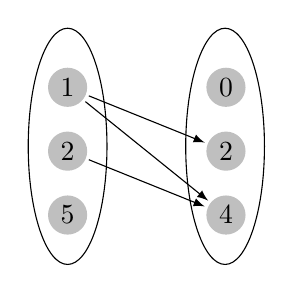
\begin{tikzpicture}
[mydot/.style={circle, fill=lightgray, inner sep=5pt}, >=latex, shorten >= 1pt, shorten <= 1pt]

% Left set:
\node[mydot,                    label={center:1}] (a1) {}; % 1
\node[mydot, below=0.3cm of a1, label={center:2}] (a2) {}; % 2
\node[mydot, below=0.3cm of a2, label={center:5}] (a3) {}; % 5
	
% Right set:	
\node[mydot, right=1.5cm of a1, label={center:0}] (b1) {}; % 0
\node[mydot, below=0.3cm of b1, label={center:2}] (b2) {}; % 2
\node[mydot, below=0.3cm of b2, label={center:4}] (b3) {}; % 4

% Arrows for the relations:
\path[->] (a1) edge (b2);                                  % 1 -> 2
\path[->] (a1) edge (b3);                                  % 1 -> 4
\path[->] (a2) edge (b3);                                  % 2 -> 4

% Ellipses around the sets:
\draw (0.0,-0.75) ellipse (0.5cm and 1.5cm);
\draw (2.0,-0.75) ellipse (0.5cm and 1.5cm);

\end{tikzpicture}
\end{figure}
% https://tikz.dev/tikz-transformations
% see:
% https://tex.stackexchange.com/questions/157450/producing-a-diagram-showing-relations-between-sets
% https://latex.org/forum/viewtopic.php?t=21987
% It's actually the "<"  relation - maybe mention it in the section about orders...but that doesn't really fit well because in orders domain and codomain are the same
There are a couple of important features that such a relation may or may not have. In a \emph{left-total} relation, every element in the left set has an outgoing arrow emanating from it. In a \emph{right-total} relation, every element in the right set has an incoming arrow. In a \emph{right-unique} relation, every element in the left set has at most one outgoing arrow. The naming convention reflects the idea that when you pick one element from the left set, the related  element of the right set, if any, is uniquely determined. We always know, where we have to go. Likewise, in a \emph{left-unique} relation, every element of the right set has at most one incoming arrow. For every element from the right set, the related element from the left set, if any, is uniquely determined. We always know, where we came from. As we can see, our example relation $R$ actually has none of these features.

\medskip
Notationally, we may write $(a,b) \in R$ when we want to express the fact that $a$ is related to $b$ by the relation $R$. Some authors write this in the shorthand infix notation $a R b$ but that looks kinda ugly. For most relations, we'll use special symbols such as $<, \leq, =, \ldots$ such that the infix notation will look nice. 

\medskip
Our example relation above was an example for a general case where we have a relation between elements of a set $A$ and elements of a set $B$. We say that $R$ is a \emph{relation between} the sets $A$ and $B$. An important special case of that is when $B$ is actually the same set as $A$. We then say that we have a \emph{relation on} the set $A$. For a relation on a set $A$, there are a couple of more important named features that the relation may or may not have. In the following table, we use the generic infix symbol $\sim$ for our relation and $\nsim$ to indicate that the elements are not in the relation. 

\medskip
\begin{tabular}{c l}
\label{Tab:RelationFeatures}
  $a \sim a$                                       & Reflexive     \\
  $a \nsim a$                                      & Irreflexive   \\
  $a \sim b \Rightarrow b \sim a$                  & Symmetric     \\
  $a \sim b \Rightarrow b \nsim a$                 & Asymmetric    \\
  $a \sim b \wedge b \sim a \Rightarrow a = b $    & Antisymmetric \\
  $a \sim b \wedge b \sim c \Rightarrow a \sim c$  & Transitive    
\end{tabular}
\medskip

When a relation is \emph{reflexive}, it means that every element $a$ must be in relation with itself. In \emph{irreflexive} relations, no element is allowed to be in relation with itself. If a relation is \emph{symmetric}, then if the tuple $(a,b)$ is in the relation, then the tuple $(b,a)$ must also be in it. If the relation is \emph{asymmetric}, such a symmetry condition is not allowed for any pair $a,b$. In an \emph{antisymmetric} relation, the symmetry condition is only allowed in the special case of $a = b$. That means, counterintuitively, that asymmetry is actually a stronger requirement than antisymmetry. Every asymmetric relation is antisymmetric but not vice versa. Asymmetry also implies irreflexivity, by the way. Finally, transitive means that if the tuples $(a,b)$ and $(b,c)$ are in the relation, then the tuple $(a,c)$ must also be in it. Some combinations of features have turned out to be important enough to warrant giving special names to those relations that have the respective combination of features. Let's now take a look at the most important types of relations that we will have to deal with throughout mathematics. ...TBC...VERIFY
% what about anti-reflexive?
% https://en.wikipedia.org/wiki/Reflexive_relation
% https://en.wikipedia.org/wiki/Intransitivity#Antitransitivity

% https://en.wikipedia.org/wiki/Connected_relation

% https://math.stackexchange.com/questions/778164/is-an-anti-symmetric-and-asymmetric-relation-the-same-are-irreflexive-and-anti


%The relation must be \emph{reflexive} meaning that every element $a$ must be in relation with itself. They must also be \emph{symmetric} meaning that if the tuple $(a,b)$ is in the relation, then the tuple $(b,a)$ must also be in it. Finally, they must be \emph{transitive} meaning that if the tuples $(a,b)$ and $(b,c)$ are in the relation, then the tuple $(a,c)$ must also be in it. Reflexivity just means that every object is equivalent to itself. 

% https://de.wikipedia.org/wiki/Asymmetrische_Relation
% https://de.wikipedia.org/wiki/Antisymmetrische_Relation
% https://de.wikipedia.org/wiki/Transitive_Relation
% https://de.wikipedia.org/wiki/Reflexive_Relation

% explain left/right totality, left/right uniqueness - see Bill Shillito's course on youtube
% use as example A = {1,2,3,4}, B = {0,2,4} and the < relation. R = {(1,2),(1,4),(2,4),(3,4)}
% not left-total due to (4,X) missing
% not right-total due to (X,0) missing
% not left-unique due to (1,4),(2,4),(3,4)
% not right-unique due to (1,2),(1,4)
% explain inverse relations
% reflexive/irreflexive, symmetric/asymmetric/antisymmetric
%   https://www.youtube.com/watch?v=GvNGf9Gki7o 
% transitive
%   https://www.youtube.com/watch?v=O19RpfoxQpA
%   make table like at the end of this video - but verify the definitions - the asymmetry
%   definition looks fishy. Maybe antimsymmtery is also "wrongly" defined there?
%   draw diagrams

% https://byjus.com/maths/relations-and-its-types/
% https://www.toppr.com/guides/maths/relations-and-functions/types-of-relations/

% https://www.youtube.com/watch?v=Tk5_B7w5fiY&list=PLZzHxk_TPOStgPtqRZ6KzmkUQBQ8TSWVX&index=9

% Was sind angeordnete Körper? (Ordnungstheorie)
% https://www.youtube.com/watch?v=RyhUIoif_B8


\paragraph{Functions} A \emph{function} is a special kind of relation, namely a relation which is \emph{left-total} and \emph{right-unique}. You can think of functions as a definition of a map from a set $A$ to another set $B$. Each element of $A$ gets mapped to some unique element of $B$. You can throw any $a \in A$ at a function $f$ and it will unambiguously tell you, which $b \in B$ your given $a$ is mapped to. If a function is additionally left-unique, we can actually traverse the arrow back to figure out unambiguously, where we came from. We can undo the application of the functional mapping for those $b \in B$ which have an incoming arrow. Such left-unique functions are also called \emph{injective}. If, on the other hand, the function is right-total, i.e. every element of $B$ has an incoming arrow, we call the function \emph{surjective}. A function that is both injective and surjective is called \emph{bijective}. There is a one-to-one correspondence between the elements of $A$ and those of $B$. Such bijective functions can therefore be uniquely inverted, i.e. undone, for any $b \in B$ and are therefore also called \emph{invertible}.

% ToDo:
% -explain domain, range, image, pre-image (of elements and whole sets)
% -give the condtions for functions in math notation
% -explain creation of binary functions
% -explain notation f: A -> B
% -explain partial functions - need not to be left-total
% -exaplain multifunctions - need not to be right-unique

\paragraph{Binary Operators} We sometimes need functions $f$ that map pairs of the form $(a,b)$ where $a$ and $b$ come from a set $A$ to another value $c$ also from the set $A$. Such a function is in certain contexts called \emph{binary operator} or \emph{binary operation} on the set $A$. Our usual arithmetic operators for addition and multiplication are of that kind. We already have all the tools to create such functions in our toolbag. We know how to create the set of tuples and we know how to create functions. Combining these two ideas, we have all the tools we need to create binary operations.

%, although the process of the creation of the set of tuples

\paragraph{Equivalences} An \emph{equivalence relation}, or in short just \emph{equivalence}, is another special kind of relation. In equivalence relations, the left and right set are actually the same set so these are relations \emph{on} a set and equivalence relations must be \emph{reflexive}, \emph{symmetric} and \emph{transitive}. Reflexivity simply means that every element must be equivalent to itself. The symmetry condition captures the idea that if $a$ is equivalent to $b$ then $b$ is also equivalent to $a$. Transitivity captures the idea that if $a$ is equivalent to $b$ and $b$ is equivalent to $c$, then $a$ is also equivalent to $c$. The prototype of an equivalence relation is the usual equality denoted by $=$ but the concept of an equivalence is more general. It is meant to capture the idea that two objects are interchangeable within a given context. They do not necessarily have to be the exact same object but certainly can be - this is ensured by the reflexivity. For some equivalence relations, we may actually use the $=$ symbol even though another relation may be meant. Sometimes alternatives like $\sim, \equiv, \simeq, \cong,$ etc. are used. The notation for various equivalence relations may vary from field to field and from author to author. 

% ToDo: Move the explanations of transitive, reflexive, etc. under the tabular

% https://www.youtube.com/watch?v=Ogm711KWwaw
% at around 14:00 The identity is the smallest equivalence relation and AxA (the "all-relation"? "universal relation" is the largest)
% https://www.ask-math.com/universal-relation.html

% https://en.wikipedia.org/wiki/Equivalence_relation
% https://mathworld.wolfram.com/EquivalenceRelation.html

\paragraph{Orders} \label{Par:Orders} An \emph{order relation}, in short just \emph{order}, is yet another special kind of relation. An order is also a relation defined on one set, i.e. the left and right sets are the same. If a set $A$ is equipped with such an order relation, the set is said to be \emph{ordered}. An order relation is typically denoted by the symbol $\leq$ which we read as "less or equal" and $a \leq b$ reads as: "$a$ is less than or equal to $b$". An order relation must be \emph{reflexive}, \emph{antisymmetric} and \emph{transitive}. Such an order can be \emph{partial} or \emph{total}, depending whether or not every pair $a,b$ can be compared via the order. In a total order, for every pair $a,b$, we always have $a \leq b$ or $b \leq a$. For a partial order, this is not necessarily the case - there may be pairs $a,b$ where neither $a \leq b$ nor $b \leq a$ is true. Total orders are also called \emph{linear orders}. A related concept is a \emph{strict order} which we typically denote by the symbol $<$ which we read as "less" and $a < b$ reads as: "$a$ is less than $b$". Such a strict order is characterized by being irreflexive, asymmetric and transitive. Note that, counterintuitively, a strict order is \emph{not} a special kind of order in the sense defined above. We required an order to be reflexive and here we require irreflexivity. These are incompatible requirements. A strict order is a different concept - but it is related to a non-strict order in the sense that given an order, one can define a corresponding strict order and vice versa. To convert between an order $\leq$ and a corresponding strict order $<$, we define $a \leq b$ to mean $(a < b) \vee (a = b)$ and we define $a < b$ to mean $(a \leq b) \wedge a \neq b$ where $a \neq b$ is a shorthand notation for $\neg (a = b)$. Strict orders can also be partial or total. Another way to characterize a strict total order is by requiring transitivity and \emph{trichotomy}. The latter means that for every pair $a,b$, exactly one of the three conditions must be true: (1) $a < b$, (2) $b < a$, (3) $a = b$.
 ...TBC...verify...explain Hasse diagram, chain
 
% https://www.youtube.com/watch?v=W8J4eEiAtIk

% https://mathworld.wolfram.com/PartialOrder.html
% https://mathworld.wolfram.com/TotalOrder.html

% https://en.wikipedia.org/wiki/Order_theory#Constructing_new_orders
% https://de.wikipedia.org/wiki/Ordnungsrelation#Totalordnung
%https://mathworld.wolfram.com/StrictOrder.html

% https://math.stackexchange.com/questions/2210560/orders-partial-orders-strict-partial-orders-total-orders-strict-total-orders

% -Strict total order: has transitivity and trichotomy, is not a "total order" because it's not
%  reflexive (this terminology is confusing!)
% -trichotomy
% -transitivity
% -it can be inverted into >
% -we have also "less than or equal to", "greater than or equal to"
% -partial and total orders 
% -well ordering - well ordered sets have a least element
% -compatibility with operations: if $a < b$ then $a + c < b + c$ for any $c \in A$

% https://en.wikipedia.org/wiki/Order_theory
% https://en.wikipedia.org/wiki/Total_order
% https://en.wikipedia.org/wiki/Partially_ordered_set#Partial_order
% https://en.wikipedia.org/wiki/Ordered_field
% https://de.wikipedia.org/wiki/Ordnungsrelation

% https://math.libretexts.org/Bookshelves/Applied_Mathematics/Seven_Sketches_in_Compositionality%3A_An_Invitation_to_Applied_Category_Theory_(Fong_and_Spivak)/01%3A_Generative_Effects_-_Orders_and_Adjunctions/1.01%3A_What_is_Order

\medskip
\medskip
We'll now shift our perspective a little bit. In the previous paragraphs, we defined certain \emph{types} of relations in terms of what properties they need to have to qualify for the given type name. The relations themselves were not specified. There may be many of them and their details may depend on the contexts. We have looked at the relations from the perspective of putting the pairs $(a,b)$ of \emph{elements} of two sets $A$ and $B$ into the relation or not. 

\paragraph{The Subset Relation} 
What we will do now is to consider the pair $(A,B)$ itself and instead of defining properties of relations, we will explicitly define some very specific relations once and for all in which any such pair of sets may or may not be. We also do not really care where $A$ and $B$ came from - whether or not they are elements from some embedding sets is not of interest here. Instead, what we want to know is if the set $B$ contains all the elements that the other set $A$ contains. In such a case, we call $A$ a \emph{subset} of $B$ and we call $B$ a \emph{superset} of $A$. The set $B$ may or may not contain more elements, i.e. elements that are not in $A$. If the superset $B$ does indeed contain additional elements, then we call $A$ a \emph{strict subset} of $B$ and we call $B$ a \emph{strict superset} of $A$. These relations are expressed with the notation $\subseteq, \subset, \supset, \supseteq$ as follows:
\begin{eqnarray}
A \subseteq B \;\;  \Leftrightarrow \;\;   x \in A \Rightarrow x \in B&           \qquad & \text{$A$ is subset of $B$} \\
A \supseteq B \;\;  \Leftrightarrow \;\;   x \in B \Rightarrow x \in A&           \qquad & \text{$A$ is superset of $B$} \\
A \subset   B \;\;  \Leftrightarrow \;\;   x \in A \Rightarrow x \in B,& A \neq B \qquad & \text{$A$ is strict subset of $B$} \\
A \supset   B \;\;  \Leftrightarrow \;\;   x \in B \Rightarrow x \in A,& A \neq B \qquad & \text{$A$ is strict superset of $B$}
\end{eqnarray}
% Alignment is ugly! Maybe use a tabular environment
In contrast to orders, equivalences, functions and so on, the subset relation is an elementary set theoretical idea and not context dependent. If it is applied to a given set of sets, it satisfies the requirements of a partial order, by the way [VERIFY].

% ToDo: maybe express the strict subset relations also as:
% (A \subset  B)  -> ... and there exists an element of of B that is not an element of A.
% The latter replaces the A \neq B condition. It's more complicated to express it that way but it communicates the intention of the definitiuon more clearly.

\paragraph{Disjointness}
Two sets $A$ and $B$ are said to be disjoint when they have no elements in common. That means formally $(x \in A \Rightarrow x \notin B) \wedge (x \in B \Rightarrow x \notin A)$. Like the subset relation, disjointness is another elementary set theoretical relation that is defined once and for all. It is not usually introduced in the context of relations, though. There is no special symbol to indicate that two sets are disjoint either\footnote{One could perhaps contemplate to use the perpendicular symbol $\perp$ for that purpose, but that is not part of standard notation}. One short way to symbolically convey that two sets $A,B$ are disjoint is via the equation $A \cap B = \emptyset$. That means that the \emph{intersection} between $A$ and $B$, i.e. the set of elements that $A$ and $B$ have in common, is the empty set. We'll properly introduce the $\cap$ symbol for set intersection later. If we have a family of sets $F = A_1, A_2, A_3, \ldots$, we say that the $A_i$ are \emph{mutually disjoint} or \emph{pairwise disjoint} when $\forall i,j: i \neq j \Rightarrow A_i \cap A_j = \emptyset$. That is: every possible pair $A_i, A_j$ of sets that we can pick from $F$ is disjoint, with the sole exception to pick the same set twice.

%  Two sets are called \emph{disjoint} when they have no elements in common.
% https://en.wikipedia.org/wiki/Disjoint_sets
% https://testbook.com/maths/disjoint-set

% -exlpain mutual disjointness of a set of sets. Sets of sets are sometimes called systems
%  https://en.wikipedia.org/wiki/Family_of_sets
% -it implies that theri intersection is empty
% -is there a symbol for it?

\paragraph{The Element Relation} 
Take again two sets $A$ and $B$, not necessarily distinct, and let $a \in A$ and $b \in B$. If the elements of $A$ and $B$ are themselves sets\footnote{In modern set theory without atomic urelements, there's nothing else they could possibly be anyway.}, then $a,A,b,B$ are all sets. That means we can ask questions like "is $A$ an element of $b$", that is $A \in b$. Or we could ask for whether or not $A \in B$ or $B \in A$ or $B \in a$, etc. We could even ask if $A \in A$ or $A \in a$ or $a \in a$. The answers to these latter questions will be "no", though because such recursive element inclusions are forbidden in axiomatic set theory - but it does make sense to ask the question. That is, our $\in$ symbol also defines a relation. The concepts in set theory begin to feel somewhat recursively self-referential by now and it is indeed the case that the whole imposing edifice of set theory somehow manages to bootstrap itself out of (almost) nothing.





\paragraph{Relational vs Operational Interpretation}
We defined a function to be a special kind of relation (left-total, right-unique) and we also intuitively characterized a function as a sort of operation with an input and an output. The operational viewpoint is the way, we usually think of functions: we put some object in and get some object out. It is important to realize that such an "operational" point of view is not necessary. From a set-theoretic point of view, the "relational" point of view is all there is: a function is just a special kind of relation and a relation is just a special kind of set consisting of ordered pairs and ordered pairs can also be thought of as being special kinds of sets (built via the Kuratowski pair construction). The definition really says nothing at all about a function being an input/output "operation". This is merely our interpretation. Or maybe it's more appropriate to say, that an input/output device is something that we want to \emph{model} with the concept of a function. At the core, it all just boils down to specific sorts of sets, because in set theory, sets are really the only thing that we have to work with anyway.

\medskip
A similar consideration can be applied to equivalences. By definition, they are also just a special kind of relation. When we use equivalences, for example to simplify equations, we sometimes interpret an equivalence as a possible replacement rule that can be applied to (parts of) a formula, i.e. a sort of operation. That's not what an equivalence is, at its core, though. It's a common misconception to think of the equals sign $=$ as a prescription to do something like an assignment or replacement when in reality, it just expresses the fact that two things are equal. An equation like $E = m c^2$ can indeed be used to compute $E$ when $m$ and $c$ are known but $E$ is yet unknown and that's indeed how we often use equations: to compute an unknown value from known ones. But the equation in and of itself, at its core and by its nature, is not an algorithmic prescription for a computation. It's just a relation.

\medskip
As we see, relations are quite flexible tools and can be used to model several important concepts in mathematics by imposing some additional requirements on the broad and general concept of a relation.
% ToDo: mention some other kind special kinds/classes of relation
% -binary operations: (A x B) -> C: combine the ordered-pair/set-product mechanism do create
%  the domain D = A x B, then use the function creation mechanism to create the desired subset
%  of (D x C), the set-product between domain and codomain

%there's not really an intrinsic input/output interpretation
%-explain the relational and operational aspects of 
% -functions (is-related vs input-output) 
% -equivalences (is-equivalent-comparisons vs assigments in programming and simplifications in math)
% -subset relations (is-a-subset vs form/extract-a-subset)
% -explain bi- and multivariate functions (using a set-product as input), 
% -functions of a scalar that yield vector outputs (parametric curves) using a set-product as output
% -explain multifunctions such as the n-th root of a complex number
% -explain the notation f: A -> B
% -explain how the interpretations of two-input/one-output functions: A x B -> C and one-input/two-output function A -> B x C can be though of as ternary relations, i.e. subsets of A x B x C where formally A -> B x C is *interpreted* as A x (B x C) and A x B -> C as (A x B) x C but the interpretation can be "flattened out" and we can do partial application, currying, etc.

% what about relational algebra? useful for databases, I think

% https://texample.net/tikz/examples/set-operations-illustrated-with-venn-diagrams/
%Cardinality

% Union set: A bing cup/union symbol U X means the union of all elements of X. We assume here that each element of X is itself a set - which in set theory is true because there are no other things than sets anyway

% https://www.youtube.com/watch?v=szfsGJ_PGQ0
% The Axiom of Choice

% https://www.youtube.com/watch?v=szfsGJ_PGQ0
% 26:00 - well ordering theorem - explain connection to statement that complex numbers can't be ordered - this seems to be a contradiction - but "being ordered" for complex numbers requires more - the order must be compatible with the arithemtic operations - this is a difference of meaning which is confusing and should be pointed out.

%---------------------------------------------------------------------------------------------------
\subsubsection{Set Operations}

\paragraph{Set Algebra} \label{Par:SetAlgebra} Just like we could combine logical propositions via the connectives $\wedge, \vee, \neg, \ldots$ to yield new propositions, there are operations that we can perform on sets to yield new sets. The \emph{intersection} of two sets $A, B$ is denoted as $A \cap B$ and defined to be the set with the elements that are present in $A$ and in $B$, i.e. the set of elements that $A$ and $B$ have in common. If the intersection between $A$ and $B$ is empty, i.e. the two sets have nothing in common, formally denoted as $A \cap B = \emptyset$, we say that $A$ and $B$ are \emph{disjoint}. The visual resemblence of $\cap$ and $\wedge$ is, of course, no coincidence. The \emph{union} of two sets $A,B$ is the set of all elements that are in $A$ or in $B$ where the "or" is again to be understood as an inclusive or. Imagine throwing all contents of sets $A$ and $B$ together into a bucket. You may get doublings for the common elements (i.e. the intersection) but that doesn't matter anyway because set membership does not care about potential multiplicities - but if you want, you can imagine to remove the doublings after throwing the sets together. The notation for the union of $A$ and $B$ is: $A \cup B$. The symbol looks a bit like a cup and resembles the "or" symbol $\vee$ from logic - again no coincidence. There is also a notion of a set \emph{difference} $A \setminus B$ which is the set $A$ minus those elements of $A$ which are also in $B$. You may read this as "$A$ take away $B$" or "$A$ without $B$" or just "$A$ minus $B$". An alternative notation is indeed to write $A - B$. It's also called the \emph{relative complement} of $B$ with respect to $A$. If we assume that we have some sort of universal set, i.e. the set of all things that we could possibly consider in the current context, we may also define the \emph{complement} of a set $A$, denoted as $\overline{A}$, which is the set of "everything" except the elements of $A$. Here, "everything" refers to our universal set which may depend on the context. If we call this universal set $U$, we could define $\overline{A} = U \setminus A$. The so called \emph{cartesian product} or \emph{set product} or \emph{cross product} or just \emph{product} of two sets $A$ and $B$, denoted as $A \times B$, is the set of all possible pairs $(a,b)$ where $a$ is an element of $A$ and $b$ is an element of $B$. Finally, the \emph{power set} operation $\mathcal{P}(A)$ takes the set of all subsets of a given set $A$. Here is a summary of these basic set operations:
\begin{eqnarray}
 \overline{A}  =& \{x: \; x \notin A \}                    \qquad &\text{complement} \\	
 A \cap B      =& \{x: \; x \in A \wedge x \in    B \}     \qquad &\text{intersection} \\
 A \cup B      =& \{x: \; x \in A \vee   x \in    B \}     \qquad &\text{union} \\
 A \setminus B =& \{x: \; x \in A \wedge x \notin B \}     \qquad &\text{difference} \\
 A \times B    =& \{(x,y): \; x \in A \wedge y \in    B \} \qquad &\text{product} \\
 \mathcal{P}(A) 
        = 2^A = &  \{x : \; x \subseteq A \}               \qquad &\text{power set}
\end{eqnarray}
The product may be iterated in the following way: Form the product $A \times B$ and then take the result of that and form the product with a third set $C$ to get: $(A \times B) \times C$. What we formally get would be a set of pairs where the first element is itself a pair of elements from $A$ and $B$ and the second element is an element from $C$. Elements of $(A \times B) \times C$ would look like $((a,b),c)$ where $a \in A, b \in B, c \in C$. On the other hand, elements of $A \times (B \times C)$ would be of the form $(a, (b,c))$. Formally, this is a different set, so our set product is formally not associative. However, the set $(A \times B) \times C$ is isomorphic (i.e. of the "same form") to $A \times (B \times C)$ and in many practical applications, what we actually want to form is not a set of nested pairs but rather a set of triples $(a,b,c)$ with no further inner structuring. We will adopt the convention that when we write a set product with multiple factors without any parentheses like: $A \times B \times C$, we mean the set of triples $(a,b,c)$ where $a \in A, b \in B, c \in C$. And this, of course, generalizes to quadruples, quintuples, etc. We will also use the notation $A^n$ to mean a set of $n$-tuples in which each element is from $A$. 

% The fact that (A x B) x C is formally not equal to A x (B x C) means that the set product is not associative. I guess we could say that it is "associative modulo an equivalence relation" (if that is a thing) if we agree that a 2-tuple of the form (a,(b,c)) is equivalent to a 2-tuple of the form ((x,y),z) if a=x, b=y, c=z. Then we interpret these two different 2-tuples as two different notations for the triple (a,b,c) = (x,y,z).

% Actually, the power set P(A) and the set 2^A of all functions from A to 2 = {0,1} are also 
% formally different sets, but there is an obvious one-to-one correspondence (see ABoST, pg. 68).
% However, often they are treated as the same thing (ToDo: verify, find examples in the literature)

% A \setminus B = A \cap \overline{A}, see https://www.youtube.com/watch?v=gHUZFXvy4yE at 4:45
% A \cap B = \overline{ \overline{A} \cup \overline{B}  }

\paragraph{Alternative Notations}

The set difference $A \setminus B$ is sometimes denoted by a regular minus sign, i.e. as $A - B$. There are also alternative notations for the set complement that we have denoted by $\overline{A}$. These include $A^\complement, A'$ and $\neg A$. These may be used in contexts where the overline notation is already occupied by another operation. For example, in topology, the notation $\overline{A}$ is often used to denote the \emph{closure} of a set, which is the set itself plus its boundary - it takes any set and turns it into a closed set (for a set that already contains its boundary, the operation does nothing). But as long as we are not dealing with topology, we'll use $\overline{A}$ for the complement of $A$.

% A' may also be used for the Cantor derivative, I think? How about using -A? That would make a lot of sense

% https://en.wikipedia.org/wiki/Complement_(set_theory)

\medskip
The power set $\mathcal{P}(A)$ may alternatively be denoted by $2^A$ where the latter notation is motivated by the observation that, if the set $A$ has $n$ elements, then the power set will have $2^n$ elements. This also explains the name "power set". We may use both notations here. The elements $x$ of the power set $2^A$ are themselves sets - namely, subsets of $A$. The empty set does also count as a subset of any nonempty set. If a set has $n$ elements, then the number of subsets with $k$ elements is given by the binomial coefficient "$n$-choose-$k$". [VERIFY, REF needed]. The fact that the power set of a finite set $A$ with $n$ elements has $2^n$ elements can also be understood as follows: For each subset, we may define a function $f$ from $A$ to the set $\{0,1\}$ which maps an element $a$ of $A$ to $1$, if the element $a$ is to be included into the subset and to $0$ if the element $a$ is not to be included. For such a function $f$, there are $2^n$ different possibilities because for each element $a \in A$ (of which there are $n$), we can choose either $0$ or $1$ as the mapped value. Including an element into a subset or not is a binary decision. We can establish a bijection between the subsets of $A$ and the set of possible functions $f: A \rightarrow \{0,1\}$, so these sets must have the same number of elements - namely, both have $2^n$ elements.

\paragraph{Less Common Operations}
In addition to these basic and most common set operations, there are a couple of more, less common ones. Some of them are:
\begin{eqnarray}
 A \triangle B =& (A \setminus B) \cup (B \setminus A)      \qquad &\text{symmetric difference} \\
 A \sqcup B    =& (A \times \{0\})  \cup  (A \times \{1\})  \qquad &\text{disjoint union} \\
 A ^ B         =& \{ f: \; B \rightarrow A  \}              \qquad &\text{functions from $B$ to $A$} 
\end{eqnarray}
The symmetric difference is what remains, if we first form the union of $A$ and $B$ and then subtract the intersection of $A$ and $B$ from that. That is, we also have: $A \triangle B = (A \cup B) \setminus (A \cap B)$. Other possible notations for the symmetric difference are $A \ominus B$ and $A \oplus B$. The disjoint union is an operation in which we throw together the contents of two sets $A,B$ while keeping the elements that came from set $A$ distinguishable from those that came from $B$ by not using the elements of $A$ and $B$ as is but rather using tuples of the form $(a,0)$ and $(b,1)$ where $a \in A, b \in B$. The appended second components serve as tags to indicate from which set the element originally came. The purpose of the disjoint union is that many desirable set theoretic constructions involving a set union work out as desired only for disjoint sets. That's why we first make the sets $A,B$ artificially disjoint via this tuple formation and then take the union of the so created sets of tuples. The disjoint union is sometimes also denoted by a simple plus sign $+$ which makes sense in the context of cardinalities which are explained below. The set of all possible functions from a set $B$ to a set $A$ is denoted by the exponential notation $A^B$. The notation $\{ f: \; B \rightarrow A \}$ is informal and intended to mean that $f$ is a function with domain $B$ and codomain $A$. The exponential notation is used for a good reason: for finite sets $A$ and $B$, the number of possible different functions from $B$ to $A$ is indeed given by $|A|^{|B|}$ where $|A|$ denotes the number of elements of $A$ and likewise for $|B|$. In the light of the notation $A^B$ where $A$ and $B$ are sets, we can also re-justify the notation $2^A$ for the power set: If we define $2 = \{0, 1\}$, as is common in axiomatic set theory, then $2^A$ is indeed the set of functions from $A$ into $\{0, 1\}$ which we have already interpreted as a sort of "membership indicator" function - so these notations are consistent.

[TODO: give a rather comprehensive list of useful set-algebraic equations, define big intersection and big union for sets of sets]

% https://en.wikipedia.org/wiki/List_of_set_identities_and_relations

% A \setminus B = A \cap \overline{A}, see https://www.youtube.com/watch?v=gHUZFXvy4yE at 4:45
% A \cap B = \overline{ \overline{A} \cup \overline{B}  }

% TODO: figure out, if there's a formal notation for the informal $A^B = \{ f: \; B \rightarrow A \}$
% notation. Maybe $A^B = \{ f \in \mathcal{P}(B \times A) : f \text{is function} \}$ as 
% semi-formal expression is ok? Here \mathcal{P}(B \times A) is the set of all possible relations
% between B and A. We then pick only those which are functions.

% ToDo: mention that the complement is sometimes also written as A^C ...with some different font for the C, mention that the complement must always be taken with respect to some universal set which may depend on the context

% https://en.wikipedia.org/wiki/Complement_(set_theory)#Relative_complement
% https://en.wikipedia.org/wiki/Disjoint_union
% https://en.wikipedia.org/wiki/Symmetric_difference
% https://math.stackexchange.com/questions/901735/meaning-of-a-set-in-the-exponent

% https://en.wikipedia.org/wiki/Exponentiation#Sets_as_exponents
% https://encyclopediaofmath.org/wiki/Exponential_law_for_sets
% A^(B x C) = (A^B)^C. This law corresponds to "currying" in functional programming

% https://math.stackexchange.com/questions/1631396/what-is-the-difference-between-disjoint-union-and-union

% Weitz uses a union symbol with a dot above to denote a union of disjoint sets. see:
% https://www.youtube.com/watch?v=RcDjuXLK-Jg&list=PLb0zKSynM2PDUcEEkjv48Y_4N9CBFyzsz&index=7
% at 9:00.  ...don't confuse this with the "disjoint union" operation which artificially makes sets disjoint before froming the union. Maybe explain both notations in the section of set theory 


\paragraph{Quotient Sets and Equivalence Classes} 
Assume we have a set $A$ and an equivalence relation $\sim$ on $A$. That is, we write $a \sim b$ whenever $a$ is equivalent to $b$ according to our equivalence $\sim$ where $a,b \in A$. Our equivalence $\sim$ \emph{partitions} the set $A$ into subsets, the so called \emph{equivalence classes}. These subsets are always mutually disjoint and their union gives us back the original set $A$. Every $a \in A$ belongs to exactly one equivalence class. No element of $A$ is missing and no element occurs more than once. This is what "partitions" means in this context. If $a$ is an element of $A$, then we denote by $[a]_{\sim}$ the set of all elements of $A$ that are equivalent to $a$ with respect to $\sim$. Formally, this means $[a]_{\sim} = \{ b \in A : b \sim a\}$. Mostly $\sim$ is clear from the context and in such cases we may just write $[a]$. The elements of such an equivalence class $[a]$ are called \emph{representatives} of $[a]$. Of course, due to the reflexivity of equivalence relations, $a$ itself is always an element of $[a]$ but any other element of $[a]$ may also serve as representative for $[a]$. They are all considered to be equivalent, after all. It may be tempting to think that $a$ is somehow the most natural and canonical representative for $[a]$, but observe that if $a \sim b$ then $[a] = [b]$ which may suggest that $b$ is just as canonical. That is, at some point, we have already made the arbitrary choice to name the equivalence class $[a]$ rather than $[b]$ and only that arbitrary choice makes $a$ look more natural as representative than $b$. Usually, we will have some means to pick a most natural representative, though. For example, if we have a strict total order on $A$ available, we could pick the smallest element of each equivalence class as representative. The set of all equivalence classes that our equivalence relation $\sim$ produces is called the "\emph{quotient set} of $A$ with respect to $\sim$". It is denoted by $A / \sim$. In a shorter language, we may also call it the "quotient of $A$ by $\sim$" or even shorter "$A$ modulo $\sim$". The surjective map that maps every $a \in A$ to its equivalence class $[a]$ is called the \emph{canonical surjection} or \emph{canonical projection}

%From each equivalence 
%is a subset

% https://en.wikipedia.org/wiki/Equivalence_class

% ~ partitions the set A. That means, it splits it into disjoint subsets that taken together give us back the whole set

% -give as example the modular integers with respect to some modulus m

\paragraph{Cardinality} While we are speaking of the number of elements of a set, i.e. the "size" of a set, it should be noted that this size has been given a special name: \emph{cardinality}. The operation of taking the cardinality of a set $A$ is denoted like taking an absolute value: $|A|$ and the result of that operation is a so called cardinal number\footnote{Cardinal numbers are, of course (you know the drill), also special kinds of sets}. We do not simply call it "size" because there are different notions of set size in mathematics and cardinality is just one of them (another one would be the so called \emph{measure}, for example). In the case of finite sets, the cardinality is just the number of elements, i.e. a natural number. That means, the natural numbers are also cardinal numbers. They are the finite cardinal numbers - but there are infinite cardinal numbers, too. And yes, that means there are different sizes of infinity in math. In a sense that can be made rigorous, there are more real numbers than natural numbers, for example. The cardinal number of the set of real numbers is bigger than that of the set of natural numbers. The notion of cardinality for infinite sets is defined in terms of existence of bijections: If for two infinite sets, you can find a bijective function between those sets, then these sets have, by definition, the same cardinality. This has a couple of counterintuitive consequences, one of which is that a strict subset of an infinite set can have the same cardinality as the whole set. The part is \emph{not} smaller than the whole. For example, the set of natural numbers and the set of even numbers have the same cardinality. The required bijection and its inverse are simply the functions $y = f(x) = 2 x$ and $x = f^{-1}(y) = y / 2$. We'll go deeper into this in a later chapter.

%But this stuff is beyond the scope of this book. [TODO: give equations for cardinalities]

%---------------------------------------------------------------------------------------------------
\subsubsection{Operations on Relations}
Now that we know what relations are and have familiarized ourselves with the common operations that we can perform on sets, we'll now have a look at some operations that we can perform on relations. In principle, since relations are just a specific kind of set, we have all the general set theoretic operations available. Of these, typically only the union, intersection and complement\footnote{If we have a relation between two sets $A,B$, the complement is taken with respect to $A \times B$. [VERIFY]} are relevant in practice. There are also a couple of specific operations that are relevant only for relations and not for general sets.

% https://en.wikipedia.org/wiki/Relation_(mathematics)#Operations_on_relations
% https://en.wikipedia.org/wiki/Algebraic_logic#Calculus_of_relations

\paragraph{Converse} The converse relation of a given relation is obtained by just swapping $x$ and $y$ in the pairs $(x,y)$ that make up the relation. For example, if $<$ is the usual less-than relation, then the converse relation would be the greater-than relation $>$. The same is true for $\leq$ and $\geq$. The relations $=$ and $\neq$ are their own converses. 
...TBC...give notations

\paragraph{Restriction}
Given a set $A$ and a relation $\sim$ on $A$ and a strict\footnote{Technically, $B$ doesn't need to be a \emph{strict} subset of $A$ but in the case $B=A$, the restriction does nothing.} subset $B$ of $A$, i.e. $B \subset A$, then we can form the restriction of the relation $\sim$ to $B$. To do this, we take $\sim$, which is a set of pairs from $A \times A$, and just remove from it all those pairs $(x,y)$ for which $x \notin B \vee y \notin B$, i.e. at least one of the components of the pair $(x,y)$ is not an element of $B$. By doing so, we turn $\sim$ into a relation on $B$
...TBC...explain left and right restriction, notations, etc.

% Is there somethin similar for relations between two different sets, i.e. we have a relation between A and B and have subsets C,D of A,B respectively - could we do something like a "birestriction"?

\paragraph{Composition}
You may be familiar with the composition of functions. From the operational point of view, such a composition would just take an input, then apply the first function to obtain an intermediate result and then apply the second function to that to obtain the final result. Functions are specific relations and the notion of composing relations is a generalization of function composition to more general relations ...TBC...

% https://en.wikipedia.org/wiki/Composition_of_relations
% https://en.wikipedia.org/wiki/Function_composition

% Containment:
% -The subset relation, when applied to relations, is called containment. A relation can be 
%  contained in another





%\section{Functions}
Functions are like machines that take some input and produce some output. In the case of mathematical functions, these inputs and outputs are usually numbers. There are more general notions, taking other types of inputs and producing other types of output, for example sets, vectors, matrices, etc. but here, we will mainly look at functions that take one number as input and produce another number as output and those two numbers will typically assumed to be real numbers. The output of a function is supposed to depend only on the input and will be uniquely defined in the sense that if you apply the same input to a function multiple times, you will always get the same output. The role of the function is to "map" the input value to its corresponding output value. That's why functions are also sometimes called maps.

% That notion of a function is different from the notion of a function in imperative programming where the output of functions can depend on all sorts of internal and external state.

% Functions may also be called "maps":
% https://en.wikipedia.org/wiki/Map_(mathematics)

%===================================================================================================
\subsection{Domain and Range}
The two sets (of numbers) from which inputs can be taken and outputs will be produced are called the \emph{domain} and \emph{range} of the function respectively. Functions are usually denoted by lowercase letters such as $f,g,h$ etc. If a function takes real numbers as inputs and also produces real numbers as output, we write this as: $f: \mathbb{R} \rightarrow \mathbb{R}$. The argument of the function is usually denoted by $x$ and and is written in parentheses and the output is often denoted by $y$. When we write something like $y = f(x)$, we mean that the function $f$ produces the number $y$ as output when we give it the number $x$ as input. An example could be $y = f(x) = x^2$. The function would just square the input and return that as result. 

%\medskip
\subsubsection{Codomain and Image}
There is a little ambiguity with respect to the notion of range. It may mean either one these two things: sometimes it may mean the set of numbers from which outputs can \emph{potentially} be drawn and sometimes the (possibly smaller) set of numbers, that can \emph{actually} be the result. For example, if the domain of $f(x) = x^2$, is taken to be the set real numbers $\mathbb{R}$, we could think of $f$ as a mapping between real numbers and real numbers, i.e. $f: \mathbb{R} \rightarrow \mathbb{R}$. However, not all possible real numbers are reached because the result of $x^2$ will never be a negative number. We could also consider $f$ as a function from the real numbers to the \emph{nonnegative} real numbers, i.e. $f: \mathbb{R} \rightarrow \mathbb{R}^+_0$. To distinguish these two notions, sometimes the term "codomain" is used for the set that outputs could potentially be drawn from and "image" is used for the set from which numbers are actually produced by the function for a given input domain. You may also find authors talk about the image of a set under a function $f$ where that set is a subset of the domain of $f$. By this, they mean the set of output values that a function produces for the given set of input values. For example, the image of the interval $[3,5)$ under $f(x) = x^2$ is the interval $[9,25)$. The converse of this is called the \emph{pre-image} which is the set of input values that gives rise to a given set of output values. The pre-image of $[9,25)$ under $f(x) = x^2$ is $[3,5) \cup (-5,-3]$, for example. You may sometimes see expressions where a set $A$ is given as an argument to a function $f$, denoted as $f(A)$ or $f[A]$. What is meant by that is the image of the set $A$ under $f$ which is again a set. For the pre-image of a set $B$, you may see notations like $f^{-1}(B)$ or  $f^{-1}[B]$. The bracket notation is actually preferable because it makes clear that a set is taken as input rather than a single (numeric) argument. However, most authors tend to use the more sloppy parentheses notation for both - single arguments and sets of arguments. This may lead to confusion in certain cases. These cases may seem contrived to the beginner but they actually may occur in practice in more advanced math contexts, so we will adopt the bracket notation here.

% https://en.wikipedia.org/wiki/Domain_of_a_function
% https://en.wikipedia.org/wiki/Range_of_a_function

% If a set is given as input to a function to produce the image set A, it is better to use bracket rather than parentheses notation, i.e f[A] rather than f(A) (Weitz explains in one of his videos why - it's in the 2023 course, the videoo about function, I think.). Here:
% https://www.youtube.com/watch?v=1DK_5koM-1o&list=PLb0zKSynM2PCLnXVwfjVcefXa6iZA-an4&index=20
% the relevant part starts at around 7:30, 14:58
% Maybe elaborate this a bit

% The codomain "contains" the set of outputs
% https://www.youtube.com/watch?v=szfsGJ_PGQ0

%===================================================================================================
\subsection{Taxonomy}
There are certain features that a function may or may not have which turn out to be important for classification. A function is said to be \emph{monotonically increasing}, if from $a \geq b$ follows $f(a) \geq f(b)$. It means that the function either goes upward or stays constant but never goes downward. If the stronger condition  $a > b \Rightarrow f(a) > f(b)$ holds true, then $f$ is \emph{strictly monotonically increasing}. Such a function really goes upward everywhere. Not even plateaus are allowed. A \emph{(strictly) monotonically decreasing} function is defined analogously with $\leq, <$ rather than $\geq, >$. If a function is either (strictly) monotonically increasing or decreasing, it is called \emph{(strictly) monotonic}. A function $f$ is said to be \emph{bounded from above} when there is some finite number $U$ such that $f(x) \leq U$ for all $x$. The number $U$ is called an \emph{upper bound} for $f$. Likewise, a function $f$ is called bounded from below, when there's some number $L$ such that $f(x) \geq L$ for all $x$. In this case, $L$ is called a \emph{lower bound} for $f$. A function that is bounded from below and above is called \emph{bounded}. A function for which we have $f(x) = f(-x)$ has \emph{even symmetry} and a function with $f(x) = -f(-x)$ has \emph{odd symmetry}. Every function $f$ can be decomposed into an even part $f_e$ and odd part $f_o$ like so: 
\begin{equation}
\label{Eq:EvenOddFuncDecomp}
f_e(x) = \frac{f(x) + f(-x)}{2}, \;\;
f_o(x) = \frac{f(x) - f(-x)}{2}, \qquad
f(x) = f_e(x) + f_o(x)
\end{equation}
\emph{Injectivity}, \emph{surjectivity} and \emph{bijectivity} are also important features which have already been discussed in the section about set theory. To reiterate, injectivity means that different inputs get mapped to different outputs: $x_1 \neq x_2 \Rightarrow f(x_1) \neq f(x_2)$. This is sometimes also called a \emph{one-to-one} mapping. Surjectivity means that all possible numbers from the codomain are reached: $\forall y \exists x: f(x) = y$. A surjective function is sometimes also called \emph{onto} - it maps them domain onto the full codomain. Bijectivity means injectivity and surjectivity, i.e. the function is one-to-one and onto. Bijective functions are \emph{invertible}. Functions can also be \emph{periodic}. That means that there exists some number $p$, called the period, such that $f(x) = f(x + k p)$ for all inputs $x$ and all integers $k$. Such a function repeats itself over and over. Functions may have \emph{asymptotes} which are straight lines which the function approaches as the argument goes to plus or minus infinity. Asymptotes can also be vertical lines. In this case, the line is approached as the argument approaches a finite value and at that value itself, the function is usually undefined. When a function $f(x)$ has a vertical asymptote at some input value $x_0$, we call $x_0$ a \emph{pole} of the function. A function is said to be \emph{compactly supported}, if it is nonzero only in some finite interval and zero outside that interval. A function is called \emph{convex} if you can pick any two points $(a,f(a)),(b,f(b))$ on its graph, connect them with a straight line and the function will be below that line everywhere. The function behaves like a chain hanging down, i.e. it is curved downward like a bowl. The opposite of convex is \emph{concave}. Such functions are everywhere above the straight line. They look like an arch. A \emph{continuous} function is one that can be drawn without lifting the pencil or drawing vertical lines. Functions can also be classified according to their degree of \emph{smoothness} and/or according to whether or not they have a finite area under their graph. To define exactly what that means, we will need a few tools from calculus (differentiability, integrability), so we will defer further discussion about these features to later chapters.

% surjective: codomain coincides with image?

%===================================================================================================
\subsection{Defining a Function}

\paragraph{Explicit Rules}
One way to define a function is to prescribe a simple \emph{calculation rule} such as $f(x) = x^2 + 3 x - 5$ that applies equally to all possible inputs $x$. Up to until a few hundred years, this was the only way that was acceptable for mathematicians to define a function. Today, we have become a lot more liberal in that regard and allow functions to be defined in more esoteric ways. Some of these ways will involve concepts that are discussed only later in the book. If you don't understand these definitions, you can skip them on a first reading. In a first pass, you need to understand only this and the next way.

\paragraph{Piecewise Definitions}
A slightly more complicated way to define a function would be to have different calculation rules for different subsets of the domain. If these subsets are succesive intervals of the real number line, this way of defining a function is called a \emph{piecewise definition}. They are written down like this:
\begin{equation}
f(x) = 
\begin{cases} 
 0 \quad& x < 0 \\
 -x     & 0   \leq x < 1 \\
 x^2    & x \geq 1
\end{cases}
\end{equation}
This means, the function will output $0$ for $x < 0$ and $-x$ when $x$ is between zero and one (including zero, excluding one) and $x^2$ when $x \geq 1$. The example function is discontinuous at $x=1$. It jumps from $-1$ to $+1$ there. At zero, it has a corner - that is: a discontinuity in its slope.

% Maybe try to put a small plot next to the definition. There's enough space

\paragraph{Conditional Definitions}
The piecewise definition is a specific kind of a conditional definition where the conditions are of the form "if $x$ is in interval ... then ...". A function can also be defined by more general conditions such as:
\begin{equation}
f(x) = 
\begin{cases} 
 1 \quad& x \in    \mathbb{Q} \\
 0      & x \notin \mathbb{Q}
\end{cases}
\end{equation}
The function given above is called the Dirichlet function or indicator function of the rational numbers. It outputs one for rational inputs and zero for irrational inputs.

\paragraph{Definition by Data}
A function can also be defined by recorded data points of some measurement. To turn these discrete data points into a continuous function, one would also have to prescribe some sort of \emph{interpolation} rule such as "connect the dots by straight lines". The data together with the interpolation rule constitute a bona fide function: we can give it an input $x$ and it will give back an output $y$. 

\paragraph{Algorithmic}
Functions can be defined by the limit of some infinite recursive process or algorithm. An example of that is Bolzano's function. Such functions will often show self-similar, "fractal" behavior: you can zoom in as much as you like and it will always look similar. 
...TBC...ToDo: explain construction rule
% https://de.wikipedia.org/wiki/Bolzanofunktion
% https://demonstrations.wolfram.com/BolzanosFunction/
% Maybe "Algorithmic" is a too general term here. Maybe use "Recursive" or "Geometric". It's basically a recursively applied geometric construction rule. Maybe "Recursively Geometric". Or "as limit"

\paragraph{Infinite Sums}
The infinite process is sometimes defined to be an infinite sum. The individual terms are defined in terms of already known, simpler functions. An example of such a definition is the Weierstrass function defined as:
\begin{equation}
f(x) = \sum_{n=0}^\infty a^n \cos(b^n \pi x), 
\qquad 0 < a < 1, \; b \in \mathbb{N}, odd, b \geq 7
\end{equation}
It has two tweakable parameters $a,b$. It is defined as an infinite sum of exponentially weighted sinusoidal functions. This function has also a self-similar nature and a couple of strange properties that were unheard of in mathematics up to the 19th century such as being continuous everywhere but differentiable nowhere.
% https://en.wikipedia.org/wiki/Weierstrass_function

\paragraph{Power Series}
Often we will encounter infinite sums of weighted powers of $x$. A function definition based on such a sum is called a \emph{power series} definition. Most of our common functions can be expressed as such a power series even though they may have originally have been constructed by other ways. Exponential and sinusoidal functions are usually first defined by means of limiting processes or geometric constructions respectively. However, they do also have power series based definitions. They can be found from the original definitions by means of a Taylor expansion. This is a topic we will discuss in more detail in the calculus chapter. This process leads to:
\begin{equation}
e^x = \sum_{k=0}^\infty \frac{x^k}{k!}, \quad
\sin(x) = ...
\end{equation}
Power series are often used to expand the domain of a function - for example, from the real to the complex numbers. This works out so nicely because all that we need to evaluate a power series is to know, how to add or multiply two objects together and how to scale an object by a factor. When we have objects on which we have these 3 operations defined, we can evaluate, for example, the exponential function of that object via the above power series. The "object" can be a real or complex number - or it can be something else such as a matrix or an operator. We'll see later what these things are. Of course, such a power series does not need to originate from already known functions. It can be made up in any way you like - you just need to prescribe some rule to compute the weights. How you came up with that rule doesn't matter. What matters is the question, whether or not the series actually converges. More on that in the section about series in the calculus chapter.

\paragraph{Analytic Continuation}
Speaking of convergence, consider the following infinite sum:
\begin{equation}
	f(x) = \sum_{n=1}^\infty \frac{1}{n^x}
\end{equation}
This sum converges only for $x > 1$. If we allow complex arguments, the condition is $\Re(x) > 1$. So in the complex plane, this sum above defines a function for those complex numbers whose real part is greater than one. For other values, the function is as of yet undefined. However, as we will see later, complex analysis provides a tool known as \emph{analytic continuation} by means of which we can uniquely expand the domain of the function to the whole complex plane except for the single point $x=1$. The so defined function is known as the Riemann Zeta function and an important object in number theory due to its unexpected connection to prime numbers. The point that I want to make here is that the process of analytic continuation gives us yet another way to define a function.

\paragraph{Continued Fractions}
Another infinite process that is sometimes useful to define a function is called a \emph{continued fraction expansion}...TBC...

\paragraph{Inverse Functions}
A function can be defined by its inverse function. In general, you can take any given function $y = g(x)$ and then define another function $f$ by asking: "for a given $y$, what $x$ would I have to plug into my function $g$ to get that $y$?". For example, the logarithm can be defined to be the inverse of the exponential function. For a slightly more interesting example, consider the function $g(x) = x e^x$. Its inverse cannot be expressed in terms of common functions. Yet, it does have an inverse (with some caveats). The inverse function of $x e^x$ is called the "product logarithm" or "Lambert-W" function and has applications in the solution of equations where an unknown $x$ appears as base and as exponent or inside and outside of a logarithm.
% https://en.wikipedia.org/wiki/Lambert_W_function
% https://en.wikipedia.org/wiki/Lambert_W_function#Applications
% y = x e^x  <->  log(y) = log(x) + x
% https://www.desmos.com/calculator/s3gxvjbovr

% $f(y) = g^{-1}(y)$
%ToDo: arcsin, ...
%$ actually, the Lambert-W function is a case of an inverse function - in this case, the inverse of x e^x. maybe for implicit functions use y e^y = x + sin(x)

% W solves the ODE: y' = y / (x*(1+y)), see:
% https://www.youtube.com/watch?v=cMZ_blqKKZU

\paragraph{Implicit Equations}
Defining a function via its inverse is a special case of an implicit function definition. In a more general setting, we could have a bivariate function of the form $g(x,y) = 0$. In the case of the product logarithm function, we would have $x = y e^y$, so $g(x,y) = 0 = y e^y - x$.  This is an equation that can be solved for $x$ on one side of the equation. That's why we can define a function in terms of the inverse of the other side. But that doesn't always have to be the case. Consider modifying the equation $x = y e^y$ to $x + x^5 = y e^y$ or, equivalently $g(x,y) = 0 = y e^y - x - x^5$. Now, we can't  solve for a single $x$ on one side. And as before, we can't solve for $y$ either. Still, we can ask: "for a given $y$, what value of $x$ can I plug into $g(x,y)$ such that it evaluates to zero?" or "for a given $x$, what $y$ ...". There doesn't have to be a solution and if there is one, it doesn't need to be unique. But if there is a unique solution, then that equation defines a function. If there are multiple solutions, we may pick one of them to be our function of interest. You can play with the function defined by $ y e^y = x + b \sin(a x)$ a bit here on Desmos: \href{https://www.desmos.com/calculator/jfxwuhot8k}{jfxwuhot8k}. Tweak the parameters $a,b$. When any of them is zero, then the function is the regular product-log function. When both are nonzero, we get a wiggly version of it. ...TBC...


% \href{https://www.desmos.com/calculator/t3t92nihws}{t3t92nihws}

% https://en.wikipedia.org/wiki/Implicit_function

% y e^y = x + x^5
% https://www.desmos.com/calculator/ekao9wnrun
% https://www.desmos.com/calculator/t3t92nihws

% y e^y = x + b sin(a x)
% https://www.desmos.com/calculator/izay7xuihf
% https://www.desmos.com/calculator/jfxwuhot8k

% y + sin(y)   = x e^x      a wiggly version of Lambert-W
% y + sin(a y) = x e^x      wiggles get stronger for a > 1, it becomes multi-valued
% https://www.desmos.com/calculator/mowoqggdpj

% x tanh(x) = y atan(y)     has two graphs
% https://www.desmos.com/calculator/9cfsbbm0d9


%Now we want to cosider functions defined by so called \emph{implicit equations}. These are equations of the form $g(x,y) = 0$ for some given function bivariate $g$. They define a set of points in the $xy$-plane. Now, we can define a function $y(x)$ by requiring that it should satisfy our implicit equation, i.e. $g(x,y(x)) = 0$ is satisfied for all $x$ in some domain. That's an implicit definition for $y(x)$. For example, we could require the following equation to hold:
%\begin{equation}
% y e^y = x \;  \Leftrightarrow \; x - y e^y = 0 
%\end{equation}
%In this case $g(x,y) = x - y e^y$. I did not make up this example. The so defined function $y(x)$ is called the "Lambert-W" function or "product-logarithm" function. 

% Move that into the Interlude:


\paragraph{Interlude - Evaluation}
Of course, an implicit definition tells us nothing at all about how we would go about evaluating $y$ for a given $x$. Nonetheless, it is a valid definition. Definitions do not necessarily need to prescribe an explicit evaluation algorithm. They are supposed to tell us \emph{what} it is, not \emph{how} we may compute it. If they do tell us how to compute it, that's a bonus. There are algorithms to solve such implicit equations though. But that's a topic for a later chapter. You may also wonder how we are supposed to evaluate functions that are defined by some infinite process. The answer is: on a computer, we cannot really represent real numbers exactly anyway. Our usual floating point numbers are always approximations. They attempt to approximate the real numbers - but can do so only up to a finite precision. So, from a practical point of view, it is good enough to be able to evaluate functions up to some given precision. For the infinite processes, that usually means that we can obtain a sufficiently precise approximation of the function by only doing a finite number of steps until we deem the result to be close enough. The best we can expect is to be precise within one ulp ("unit in the last place"). Usually, we'll accept even much higher errors.





\paragraph{Functional Equations}
Now let's consider the factorial function $n! = 1 \cdot 2 \cdot 3 \cdot \ldots \cdot n$. As it stands, it's defined only for natural numbers. There is a way to define it for all real and even complex numbers. The key lies in the observation of the factorial's functional equation\footnote{A functional equation is an equation that relates values of a function at different evaluation points (VERIFY!). Here, it relates the values of the factorial function at the evaluation points $n$ and $n-1$.} which is given by $n! = n \cdot (n-1)!$. In our expanded definition, we want that equation to be satisfied for all real inputs. So we search for a continuous function $f(x)$ for which the functional equation $f(x) = x \cdot f(x-1)$ holds true. It can be shown that the following integral based definitions:
\begin{equation}
\Pi(x)    = \int_0^\infty t^x e^{-t} \, dt, \quad
\Gamma(x) = \Pi(x-1) = \int_0^\infty t^{x-1} e^{-t} \, dt,
\end{equation}
do indeed lead to functions that satisfy the desired functional equation. The first definition agrees with the factorials at the naturals, i.e. $\Pi(x) = x!$ for $x \in \mathbb{N}$. That means, it interpolates (i.e. makes continuous) the formerly discrete factorial function. The second definition is called the \emph{gamma function} and it agrees with the shifted factorial function. There is some discussion on \href{https://math.stackexchange.com/questions/1362523/why-is-the-gamma-function-off-by-1-from-the-factorial}{stackexchange} about why the gamma function might have been defined with that strange shift. Supposedly, it will make some higher level stuff more convenient but at first, it seems more unnatural and inconvenient than the $\Pi$ function. Nevertheless, it's the gamma function that is used in math all over the place. Anyway, my point here is that a function definition can be based on a functional equation. 
[VERIFY all of this!]

% Differentiating The FACTORIAL?! | Laid Back Math, Episode 20
% https://www.youtube.com/watch?v=gQKc308e-R4
% has good derivation for why gamma satisfies the functional equation of the factorial

\paragraph{Parameter Integrals}
In this case of the factorial function, the solution of the functional equation led to a definition in terms of a \emph{parameter integral} which is an integral in which the integrand depends on a parameter - here $x$.
I think, the general way to define a function $f$ in terms of a parameter integral is to have some function $g(x,t)$ and then use:
\begin{equation}
 f(x)  = \int_{a(x)}^{b(x)} g(t,x) \, dt
\end{equation}
For $\Pi(x)$ we have $g(x,t) = t^x e^{-x}, a(x) = 0, b(x) = \infty$.
[VERIFY all of this!]
...TBC...
% https://en.wikipedia.org/wiki/Gamma_function
% https://math.stackexchange.com/questions/1362523/why-is-the-gamma-function-off-by-1-from-the-factorial
% https://mathoverflow.net/questions/20960/why-is-the-gamma-function-shifted-from-the-factorial-by-1
% https://de.wikipedia.org/wiki/Parameterintegral
% Arens pg 409 ff, Bärwolff pg 166 (1 example),

\paragraph{Antiderivatives}
Speaking of integrals - we sometimes have a known function $f$ and want to define another function $F$ as an antiderivative of $f$. An important example is the area under a Gaussian bell curve from minus infinity up to some value $x$:
\begin{equation}
 F(x)  = \int_{-\infty}^{x} e^{-t^2}  \, dt
\end{equation}
I think, this can also be seen as another special case of a "parameter integral" definition with $g(x,t)=e^{-t^2}, a(x)= -\infty, b(x)=x$? ...figure out! Explain the erf-function

\paragraph{Differential Equations}
Finding an antiderivative is a problem of the form: for a given $g(x)$, find a function $f(x)$ such that $f'(x) = g(x)$. That equation is actually a special case of a more general class of equations called differential equations. These are equations in which the unknown function $f$ and derivatives of it may appear. A function $f$ that satisfies the differential equation is called a solution of the differential equation. Of course, saying something like: "let $f$ be the solution to the following differential equation..." is also a way of defining a function. There are some caveats, though: differential equations typically have many solutions so we need some additional constraints (typically boundary conditions or initial conditions) to pick out one of those solutions uniquely ...TBC...give examples for how exp and sin can be defined by an ODE, mention Bessel functions
%Having seen how function can be defined via integrals, the next step is consider functions that are defined by differential equations...TBC...

% differential equations - start with simple examples like exp, sin, cos, the give more complex examples like Bessel

\paragraph{Integral Equations}
An integral equation is an equation where an unknown function $f$ appears under an integral sign. Like with differential equations, solving the integral equation amounts to finding $f$. For example, imagine that we have two known functions $g, h$ and we want to find $f$ such that:
\begin{equation}
 \int_a^b f(u) h(x-u) \, du = g(x)
\end{equation}
for some constants $a,b$ (which are often minus and plus infinity). We could interpret $g$ as a recorded signal, $h$ as the impulse response or "kernel" of a filter and we want to reconstruct $f$ as it was before it went through the filter. The desired function $f$ appears under a convolution integral. This sort of equation is a particular kind of integral equation and does indeed define a function $f$.

%...TBC...
%ToDo: bring an example involving deconvolution - we are given a signal $g(x)$ which is supposed to be our desired $f(x)$ convolved with some known kernel $h(x)$. Then $f(x)$ appears under the convolution integral. Finding it involves deconvolution...can perhaps be done in the Foruier domain - but that's not the problem of the definition




%\paragraph{Implicit Differential Equations}
% well - so far we have said nothing in the paragraph about diffeqs that restricts us to explicit ones so we may consider the implicit ones to be already subsumed

%What about an implicit differential equation

% Yet another way to define a function:
% https://www.youtube.com/watch?v=U_5JDWR0HiM  Why care about infinite dimensions?
% it uses an (contraction) operator and defines the function as a fixed point of that operator. This coudl aczually be easily implemented numerically, I think.

\paragraph{Fixed Point of an Operator}
This is a fun one and rather exotic and requires some higher level math concepts, so feel free to skip it on a first read. An operator is a higher order function - an object that takes a function as input and returns another function as output. Such operators can have fixed points. These are functions for which the operator returns the input function unchanged - just like the function $f(x) = x^2$ has the fixed point $1$, i.e. returns one when plug in one. With such an operator in hand, we can define the function to be a fixed point of our given operator. 

% x^2 has the other fixed point x=0. x=0 is stable and x=1 is unstable, I think.

\paragraph{A Non Function}
Consider the following nonsensical looking attempt of defining a function:
\begin{equation}
f(x) = 
\begin{cases} 
0       \quad& x \neq 0 \\
\infty       & x = 0
\end{cases} \qquad \text{with} \qquad
\int_{-\infty}^{\infty} f(x) \, dx = 1
\end{equation}
We are trying to define a "function" that is zero everywhere except at zero. There, it should have an infinitely tall and infinitely thin spike. The (infinite) height of the spike should be adjusted in such a way that the total area under the function is unity. This "function" is called the Dirac delta function - and it isn't really a function at all because the definition does not really make sense formally. But when this strange function-like object appears under an integral, it suddenly starts to make a lot of sense and is very useful. We'll meet this bizarre Dirac spike again later in the chapter about functional analysis where it will be more rigorously defined as a \emph{distribution} which is a certain kind of \emph{functional}. Especially in physics and signal processing, we often work with this thing informally as if it were a function.


%ToDo: integral equation
% maybe make these subsubsection of an "Elementary functions"  section

\paragraph{Whoa!} That was a tour de force! I have presented quite a lot of ways how a mathematical function can be defined. Some of them required some rather high level math which doesn't really belong into such an early chapter. I did this to point out that the idea of "defining a function" can, when intepreted liberally as we do in the modern world, include much more diverse and creative ways rather than just a simple and explicit calculation rule. However - most functions that we encounter in everyday life are not of such a complicated nature. There's a set of functions that tends to pop up everywhere and constitutes a sort of basic mathematical vocabulary that everybody needs to be familiar with. I'm talking about the so called...

%===================================================================================================
\subsection{Elementary Functions}
In general, a function can be any mapping. But there is a certain set of functions that permeates mathematics so thoroughly that it has been given a special name: the elementary functions. These are all functions that can be constructed by a finite formula involving only the 4 basic arithmetic operations, roots, exponentials, logarithms, trigonometric functions and the inverses of all these functions.

% https://www.youtube.com/watch?v=l6w868U8C-M
% https://en.wikipedia.org/wiki/Elementary_function

%---------------------------------------------------------------------------------------------------
\subsubsection{Absolute Value aka Norm}
A simple but very important function is the \emph{absolute value} or \emph{norm} of some number $x$ which we commonly write as $|x|$ and read as "absolute value of $x$" or in some contexts also "norm of $x$". The former term applies to real numbers $x$ and the latter term applies in cases where $x$ is a more complicated object than a real number. Yes - that means the absolute value (or norm) function will later be generalized to more complicated objects (complex numbers, vectors, matrices, etc.) and by doing so, it will retain some of its important properties and that's perhaps the chief reason why it is such an important function despite being so humble. For a real number $x$, it can be defined as:
\begin{equation}
 |x| = \sqrt{x \cdot \overline{x}} = 
\begin{cases} 
  x \quad & \text{iff } x \geq 0 \\
 -x \quad & \text{iff } x   <  0 \\
\end{cases} 
\end{equation}
The piecewise definition on the right hand side is how we usually think of $|x|$ when $x$ is a real number. The definition with the square-root in the middle can at this point be taken as a provision for later generalizations and you don't need to worry about this right now, if it doesn't make any sense yet (spoiler: the overline will be used for complex conjugation and the product will generalize to a so called scalar product). Our absolute value function satisfies the following conditions for all $x,y \in \mathbb{R}$:

\medskip
\begin{tabular}{l l}
Non-negative:         & $|x| \geq 0$  \\
Positive definite:    & $|x| = 0 \Leftrightarrow x = 0$  \\
Multiplicative:       & $|x \cdot y| = |x| \cdot |y| $  \\
Triangle inequality:  & $|x + y| \leq |x| + |y| $
\end{tabular}
\medskip
%https://en.wikipedia.org/wiki/Norm_(mathematics)
% Die rationalen Zahlen liegen dicht (wie feiner Staub) in der Menge der reellen Zahlen
% https://www.youtube.com/watch?v=lWTf_Isveso

The idea of a norm function is that it should somehow measure the "size" of the object that it is being applied to. The first two conditions say that a norm can never be negative and it is zero if and only if the input is itself already zero. These conditions do indeed sound like some minimum requirements that we expect such a "norm" function to have if it should be interpretable as a size. Multiplicativity and triangle inequality are less obvious. The latter basically means that a direct path is always shorter than a roundabout path. We'll say more about this when we will meet vectors. These four are the properties that all functions shall have if they want to deserve to qualify for calling them a "norm" even when $x$ and $y$ can later be more complicated objects than real numbers. Some more properties immediately follow from these: $|x/y| = |x|/|y|$, $|x-y| = |x| + |y|$, $\bigl| (|x|-|y|) \bigr| \leq |x \pm y|$. In programming languages, the absolute value function is often called "abs". % and we may use that term as convenient abbreviation. 

\paragraph{The Signum Function}
A related function is the so called signum or sign function. It is the counterpart to the absolute value function in the sense that in contains precisely the information that was thrown away when applying the absolute value function - namely, the sign of the number. For real $x$, it is defined as:
\begin{equation}
\sign(x) = 
\begin{cases} 
 -1 \quad & \text{iff } x < 0 \\
  0 \quad & \text{iff } x = 0 \\ 
  1 \quad & \text{iff } x > 0 \\
\end{cases} 
\end{equation}
To reconstruct our original $x$, we can combine sign and norm: $x = \sign(x) \cdot |x|$. If we want to generalize that reconstruction property to more complex objects, we could define it via this relation: $\sign(x) = x / |x|$ (for $x \neq 0$). This is non-standard notation though and the term "sign" doesn't make sense if $x$ is not a real number. In the case where $x$ is a complex number or a vector, it would make more sense to call the quantity $x / |x|$ a "direction" which generalizes the idea of a "sign" (which can encode precisely two directions like "left" and "right" (and "none" as edge case for zero)).

\paragraph{Note}
I said formerly that an "elementary" function can only use the arithmetic operators, roots, the exponential and trig functions and the inverses of all of these. I didn't say anything about piecewise definitions, so one might reasonably question whether the absolute value and sign should qualify as "elementary". But the definition of the norm as $|x| = \sqrt{x^2}$ saves the day (in the reals, we have $\overline{x} = x$). Likewise, the (re)definition $\sign(x) = x / |x|$ saves the day for the sign function. We may need to make an exception for $x = 0$ though and maybe I'm being a bit sloppy here and maybe strictly speaking, the sign should not be listed in this category. But at least, it's certainly piecewise elementary.

% Zusammenhang zwischen normierten, metrischen und topologischen Räumen
% https://www.youtube.com/watch?v=3j8GIJd5-3A&list=PLHi0WgifODX19zsJhvCrizYEXiHY5qc9n

%---------------------------------------------------------------------------------------------------
\subsubsection{Complex Conjugation}

% -can be dragged out of sums and products
% -sqrt(z * conj(z)) = |z|

%---------------------------------------------------------------------------------------------------
\subsubsection{Polynomials}
A \emph{polynomial} can be written in various forms. Some important canonical forms are: (1) a weighted sum of integer powers of $x$, (2) a (scaled) product of so called linear factors, (3) a nested expression. So, a polynomial is a function of one of the forms:
\begin{equation}
 f(x) = \sum_{k=0}^n a_k x^k 
      = a_n \prod_{k=1}^{n} (x - r_k)
      = a_0 + x(a_1 + x(a_2 + \ldots + x(a_{n-1} + x a_n)))
\end{equation}
where the weights $a_k$ in the sum form are called the \emph{coefficients} of the polynomial and the highest power $n$ for which there is a nonzero coefficient is called the \emph{degree} of the polynomial and the coefficient $a_n$ in front of it is called the \emph{leading coefficient}. The $r_k$ in the product form are called the \emph{roots} of the polynomial. These are the values of $x$ where the output of the function $y = f(x)$ is zero. This is immediately obvious from the fact that a product is zero as soon as any of its factors is zero, which will clearly be the case if $x = r_k$ for one of the $r_k$. The roots $r_k$ may be real or complex and are not necessarily distinct. The number of times by which a root appears in the product is called the \emph{multiplicity} of the root. An important theorem, the \emph{fundamental theorem of algebra}, states that every polynomial of degree $n$ has exactly $n$ such roots in the complex plane (counted with multiplicity, i.e. a double root counts twice, etc.). You will sometimes find a weaker form of this statement called fundamental theorem of algebra, namely the statement that each polynomial of nonzero degree has a root. But the stronger statement immediately follows from the possibility of splitting off a linear factor. It's usually preferable for a theorem to make the most precise and strongest possible statement from the weakest possible assumptions unless, perhaps, doing so would get in the way of comprehensibility. But that's not the case here so that's why I prefer the stronger version of the theorem that I stated first. By the way, the scaling factor $a_n$ in front of the product form is indeed the same $a_n$ as the $a_k, k=n$ coefficient in the sum form, i.e. the leading coefficient. Also, the $a_k$ in the nested form are the same coefficients as in the sum form. A polynomial of degree 1, i.e. a function of the form $f(x) = a_0 + a_1  x$, is a very simple special case which is of practical importance and is sometimes - somewhat inconsistently - called a linear function. This terminology is inconsistent because such a function satisfies the usual requirements for linearity - homogeneity and additivity - only when the additive constant is zero, i.e. when $a_0 = 0$. Nevertheless, you'll find that terminology used often, especially in high-school level math texts. That's because in these contexts, what they usually mean by "linear" is: "defines a line" rather than these more abstract homogeneity and additivity properties. In more advanced university-level texts, they may also be called \emph{affine} functions. In this context, "affine" usually means: "linear plus some offset". The practical importance of such affine functions is that we will often use them to approximate more complicated functions - a process known as linearization. A polynomial of degree 2, i.e. a function of the form $f(x) = a_0 + a_1 x + a_2 x^2$, is also called a quadratic polynomial. Such polynomials are often used to approximate an arbitrary function around a minimum or maximum in the context of optimization problems. They can also be used as a more accurate approximation than linear ones around arbitrary points. Polynomials are generally used to do all sorts of approximations because polynomials are often much easier to deal with than other types of functions - especially when it comes to problems involving some calculus because polynomials are easy to integrate and differentiate in closed form.

% quadratic approximations, biquads

\paragraph{Powers and Monomials}
The individual terms of the polynomial in its sum form, i.e. the $a_k x^k$ are called \emph{monomials}. If the coefficient $a_k$ is one, we are just dealing with a integer power of $x$ where the exponent is a natural number. There are some important rules for such natural powers of $x$:
\begin{equation}
\label{Eq:PowerRulesNatural}
x^n x^m = x^{n+m}, \qquad
\frac{x^n}{x^m} = x^{n-m}, \qquad
(x^n)^m =  x^{n m} =  (x^m)^n
\end{equation}
where the second rule, for the time being, makes only sense when $n-m$ is natural, i.e. $n \geq m$. We will see later that this restriction can be dropped, though. But for that, we need to \emph{define} what $x^a$ is supposed to mean when $a$ is not necessarily natural.
% ToDo: list power rules x^{n+m} = x^n x^m,  x^{n m} = (x^n)^m
% exlpain the term "monic"

\paragraph{Evaluation}
The evaluation of a polynomial is best done in nested form. This is the computationally most efficient way and also one of the most stable ways numerically. We assume that a polynomial of degree $n$ is represented in the computer as a list or array of $n+1$ coefficients $a_0, \ldots, a_n$.
\begin{lstlisting}
def polyEval(p, x):
	"""Evaluates the polynomial p at the given x using Horner's algorithm"""
	k = len(p)-1           # last valid index
	if(k < 0):
		return 0
	y = p[k]
	while(k > 0):
		k -= 1
		y = y*x + p[k]
	return y
\end{lstlisting}
This way of evaluating a polynomial is also known as Horner's rule.
...hmm...not sure, if code should appear in the normal text. maybe put it into an appendix? 


\paragraph{Addition and Subtraction}
Polynomials, given as arrays of coefficients, can be added and subtracted element wise. If the input arrays are of different length, i.e. the polynomials are of a different degree, the lower degree coefficient array has to be padded with zeros to match the length of the larger one.
%...python code is buggy

\paragraph{Multiplication}
When we multiply two polynomials $f(x), g(x)$ with degrees $m,n$ together, we will get a new polynomial of degree $m+n$. The coefficients of this new polynomial can be found by an algorithm called \emph{convolution}. Let's see how this would look like:
\begin{eqnarray}
&  (a_0 + a_1 x + a_2 x^2 + a_3 x^3 + \ldots)
   (b_0 + b_1 x + b_2 x^2 + b_3 x^3 + \ldots)  \\
=&  c_0 + c_1 x + c_2 x^2 + c_3 x^3 + c_4 x^4 + c_5 x^5 + c_6 x^6 + \ldots \\
=&  a_0 b_0 \\
&+ (a_0 b_1 + a_1 b_0) x \\
&+ (a_0 b_2 + a_1 b_1 + a_2 b_0) x^2 \\
&+ (a_0 b_3 + a_1 b_2 + a_2 b_1 + a_3 b_0) x^3  \\
&+ (a_0 b_4 + a_1 b_3 + a_2 b_2 + a_3 b_1 + a_4 b_0) x^4 \\
&+ (a_0 b_5 + a_1 b_4 + a_2 b_3 + a_3 b_2 + a_4 b_1 + a_5 b_0) x^5 \\
&+ (a_0 b_6 + a_1 b_5 + a_2 b_4 + a_3 b_3 + a_4 b_2 + a_5 b_1 + a_6 b_0) x^6 + \ldots
\end{eqnarray}
[TODO: suppress numbering for the individual lines] \newline
The coefficient $c_n$ in the resulting polynomial is the sum of all products of input coefficients $a_i, b_j$ such that $i+j = n$. Let's introduce another index $k$ to replace $i$ and then use $n-k$ to replace $j$. This ensures that $k + (n-k) = n$. We now have:
\begin{equation}
  c_n = \sum_{k=0}^n a_k b_{n-k}
\end{equation}
That formula to compute the new list of $c$-coefficients from the $a$- and $b$-coefficients is called convolution. Multiplication of two polynomials is achieved by convolving their coefficient lists (yes, the noun is \emph{convolution} and the verb is \emph{convolve} - not convolute). Convolution is an important mathematical operation that crops up in different variations everywhere. Polynomial multiplication is just one of the many places. Signal processing is full of it. Its continuous variant plays a role in the solution of certain differential equations which are all over the place in physics. You may have learned in high school how to do polynomial multiplication with pencil and paper and you have probably hated it just as much as your seatmate and everybody else including me. Don't worry - we don't do such things here. Instead, we teach a computer to do that boring calculation for us.

...TBC... give Python code for convolution
% \bigl(\sum_{n=0}^N  a_n x^n\bigr) \bigl( \sum_{k=0}^M b_k x^k \bigr) = $\sum_{n=0}^{N+M} c_n x^n, wher c_n = ...
% give a similar formula also for nesting and deconvolution

\paragraph{Division}
Let's now see, if we can reverse the process. Let's assume that we know the coefficient arrays $c_n$ and $b_n$ and want to figure out all the $a_n$. We need to make sure that the coefficients for like powers of $x$ match. For example, at the top of the triangle, we have the product $a_0 b_0$. That's how we computed the coeff for the constant term in the product polynomial $c_0$. So we have $c_0 = a_0 b_0$. That actually already tells us $a_0 = c_0 / b_0$. Now look at the line immediately below the tip of the triangle. The sum in brackets must equal $c_1$. But $c_1 = a_0 b_1 + a_1 b_0$ means $a_1 = (c_1 -a_0 b_1)/b_0$. We have found our next coefficient! Everything on the right is already known, The $b$- and $c$-coeffs are assumed to be known anyway and $a_0$ has just been computed in the previous step. One line more to establish the pattern: we must have $c_2 = a_0 b_2 + a_1 b_1 + a_2 b_0$ so we have $a_2 = (c_2 - a_0 b_2 - a_1 b_1)/b_0$. In general:
\begin{equation}
a_n = \frac{1}{b_0} (  c_n - \sum_{k=0}^{n-1} a_k b_{n-k} ) 
\end{equation}
[...but there's a caveat: what, if $b_0 = 0$? Maybe we should find $m$ as the index of the first nonzero $b$-coeff and use $b_m$ as divisor? I think, the upper limit of the sum can then be reduced to $n-m-1$. -> figure out! What about polynomial division with remainder? Maybe apply the deconv-algo to sequences $c_n, b_n$ where $c_n$ actually did \emph{not} arise from a product involving $b_n$? Point out the caveats and provide working code that takes care of them!]


%Oh my dog! Polynomial division! That pesky algorithm that we all once had to learn in school and then have forgotten for good! Worry not - you won't have to relearn it here and now. Executing algorithms with pencil and paper is not something we humans like to do and I personally find it as pointless as the next guy. Instead, I'll give you computer code for it, so we'll never ever have to do it again by hand. ....

% what if c = 1, b = 1 + x^2 - what a would we get by deconv? maybe some sort of polynomial approximation of 1 / (1 + x^2)? We get a0 = 1, a2 = -1, a4 = +1. I guess all odd coeffs are zero and the +-1 pattern for the even coeffs continues? Figure out! But it does indeed look like taking more such terms improves the approximation, see:
% https://www.desmos.com/calculator/7rekjnfmtw
% move this comment to the cpp code where we implement or test this deconv algo - make an experiment! Compare coeffs to Taylor coeffs and the Approximation to the Taylor approximation!

\paragraph{Composition}
We can also compose two polynomials in the sense that we take an input $x$, then first apply one polynomial $y = p(x)$ and to the result $y$, we then apply another polynomial $z = q(y) = q(p(x))$. The so defined function will be yet another polynomial. When $p$ has degree $m$ and $q$ has degree $n$, then the nested polynomial defined by $q(p(x))$ will have degree $m n$.

TODO: give algorithm for computing the coeffs of the nested polynomial in terms of coeffs of the two input polynomials

% degree is m n

%..tbc..
% product form, fundamental theorem of algebra, linear functions as special case
% factor out a linear factor, polynomial addition, multiplication, division - maybe with (pseudo) code or better: sage code, maybe provide als sage code for basic integer arithmetic - maybe in the section numbers in 

%\paragraph{$\star$ Companion Matrix}
% https://en.wikipedia.org/wiki/Companion_matrix
% https://en.wikipedia.org/wiki/Minimal_polynomial_(linear_algebra)


% Sturmsche Kette: Die exakte Anzahl der Nullstellen jedes Polynoms
% https://www.youtube.com/watch?v=gG7B1KQSg_I
% -Am Ende: Cauchy's Nullstelleninterval: Sei: M = 1 + max(a_0,a_1,..,a_{n-1}) / a_n. Dann liegen
%  die Nullstellen in [-M,M]

%---------------------------------------------------------------------------------------------------
\subsubsection{Rational Functions}
A rational function is a ratio or quotient of two polynomials, i.e. function of the form:
\begin{equation}
 f(x) = \frac{\sum_{k=0}^n a_k x^k}{\sum_{k=0}^m b_k x^k}
\end{equation}
Functions of that form...TBC...

% poles, zeros, cancellation

\paragraph{Partial Fraction Expansion}

% Maybe Polynomials and rational functions should get a section in their own right. Maybe after Linear Algebra...or maybe before it. Maybe is should be called "Polynomial Algebra" and be framed as another generalization of "Linear Algebra" where "Multilinear Algebra" is the other generalization. Polynomials do not necessarily need to be interpreted as functions - we can also interpret them as formal expressions. This interpretation can be generalized to non-convergent power series. The section should also consider multivariate polynomials. OK - it is now a section the Abstract Algebra chapter



%---------------------------------------------------------------------------------------------------
\subsubsection{Arbitrary Powers of $x$}
Polynomials are constructed as linear combinations (i.e. weighted sums) of nonnegative integer powers of the independent variable $x$. Surpassing the world of polynomials, we could also allow negative integer powers and identify the resulting functions as special cases of the rational functions. That is, it makes sense to define the function $f(x) = x^{-n}$ where $n > 0$ as the simple rational function $f(x) = \frac{1}{x^n}$. It can be verified that with such a definition, our rules given in (\ref{Eq:PowerRulesNatural}) continue to hold. This definition is an example of applying the \emph{principle of permanence} which says that, whenever we extend an existing definition to a larger domain, we should strive for doing it in such a way that our old rules continue to hold in this larger domain. Here, we extended the domain for allowed exponents from the natural to the integer numbers. Now we will generalize even more and look at what happens when we allow the exponent to be a rational, real or even complex number. That means, we are now interested in functions of the general form $f(x) = x^a$ where, $a$ is not restricted to a integer anymore. Let's start by investigating what $f(x) = x^{\frac{1}{n}}$ for positive natural $n$ could mean. The principle of permanence forces our hand to define this as $x^{\frac{1}{n}} = \sqrt[n]{x}$.

...TBC...

% https://en.wikipedia.org/wiki/Principle_of_permanence

% Use a^x = e^{x \ln (a)}, x^a = e^{a \ln (x)}

% Secret Kinks of Elementary Functions:
% https://www.youtube.com/watch?v=92wXQYcYLMg  
%
% What is the graph of x^a when a is not an integer? An unusual look at familiar functions #some2
% https://www.youtube.com/watch?v=_lb1AxwXLaM  






%---------------------------------------------------------------------------------------------------
\subsubsection{Algebraic Functions}
The set of algebraic functions contains all the functions that can be constructed from using the elementary operations and extracting roots....
% partial fraction expansion








%---------------------------------------------------------------------------------------------------
\subsubsection{Exponential Functions}
A general exponential function is a function of the form $y = f(x) = b^x$ for some constant $b$ which is called the basis (or base) in this context. Choosing Euler's number $\e = \lim_{n \rightarrow \infty} (1 + 1/n)^n = 2.71828\ldots$ as basis, we obtain \emph{the} exponential function $y = f(x) = \e^x = \exp(x)$. It can be defined via a power series, a limit or as inverse of a parameter integral [VERIFY the last]:
\begin{equation}
\e^x 
= \exp(x)
= \sum_{n=0}^{\infty} \frac{x^n}{n!}
= \lim_{n \rightarrow \infty} \left( 1 + \frac{x}{n} \right)^n, \quad
x = \int_1^y \frac{1}{t} \, dt
\end{equation}
% maybe replace the y in the parameter integral by e^x. I think, that is, what it means
% give continuous fraction expansion
It satisfies the following differential equation\footnote{Don't worry if you don't know what a differential equation is - we'll learn about them later and you can ignore it for now} and functional equation:
\begin{equation}
\frac{d}{dx} \e^x = \e^x, \quad
\e^{x+y} = \e^x \e^y
\end{equation}
This functional equation is pretty interesting indeed. It means that the exponential function translates between our two most important arithmetic operations addition and multiplication \footnote{subtraction and division are less important because they can be seen as mere inverses of the more fundamental operations of addition and multiplication}. The differential equation is quite noteworthy as well. It means that the exponential function is its own derivative. We can also insert complex arguments into the series definition. The resulting series will converge for any complex number $z$ whatsoever and the properties mentioned above continue to hold.

\medskip
In the complex domain, the exponential function also subsumes the - undeniably also very important - trigonometric functions sine and cosine that are so intimately related to the circle. All of these features are quite remarkable and secure the exponential function a top spot in the hall of fame of all functions in mathematics. It is even widely regarded as the most important function in all of mathematics and the chief reason for this is its functional equation, i.e. its ability to translate between addition and multiplication.

% Other properties:
% -it produces positive real output for real inputs
% -it never produces zero as output ...except for z = -inf - but this doesn't count because 
%  -inf is not a number?
% -for real x > 0, exp(x) > 1
% -exp(x) is strictly monotonically increasing on the real number line

[TODO: give formulas for change of basis, $(\e^x)^y = \e^{x y} = (\e^y)^x$, iff $xy = yx$, i.e. multiplications is commutative - which is true for complex numbers but may not be true in other number systems, explain how the exponential function can be generalized to other number systems using the power series, But: $(a^b)^c \neq a^{(b^c)}$ - exponentiation is not associative]

%As we will learn later, a   ...?...what did I want to write here?

% As we will learn later in functional analysis, it says that the exponential function is an eigenfunction of the derivative operator. 

% Verify:
% In terms of group theory, the exponential function $\e^x$ an isomorphism between the groups $(\mathbb{R}^+, +)$ and $(\mathbb{R}^+, \cdot)$. ..I think, all epxonential functions are such an isomorphism but the basis e is the only one with the special property that...what? It is its own derivative (without a scale factor)

% https://de.wikipedia.org/wiki/Exponentialfunktion
% https://en.wikipedia.org/wiki/Exponential_function

% https://en.wikipedia.org/wiki/E_(mathematical_constant)

% Make a paragraph about 0^0. List arguments for defining it as 0, as 1 or as undefined, see:
% https://www.youtube.com/watch?v=UW2VbHDnW5w
% https://www.youtube.com/watch?v=jNhjB4UfR9A
% https://www.youtube.com/watch?v=O8aKKKdQmxY


% Die wichtigste Funktion der gesamten Mathematik
% https://www.youtube.com/watch?v=zWBQXzjj5fY

% Permanenzprinzip:
% Rechenregeln sollen weiterhin gelten bei asuweitung des Definitionsbereichs

% https://www.youtube.com/watch?v=lXYxZBSkKLU
% Euler's number
% e   = lim n -> oo (1 + 1/n)^n
% 1/e = lim n -> oo (1 - 1/n)^n
% e   = sum_n  1/n!


% Die schönste Formel der Mathematik, die Kreiszahl Pi und die trigonometrischen Funktionen
% https://www.youtube.com/watch?v=-PYEguPdwdk
% 7:37  conj(e^z) = e^conj(z)


% Maybe motivate the power series expansion through Taylor series - but that requires calculus - maybe do it in the section about Taylor series. Motivate it from trying to approximate a function and a certain number of its derivatives at a point


\paragraph{Logarithms}
We have seen that the exponential function $f(x) = \e^x$ is injective, i.e. maps different inputs to different outputs. It is not surjective on $\mathbb{R}$ though, because the negative values are never reached by $f$. However, if we restrict its codomain to $\mathbb{R}^+$, i.e. to only those values that are actually reached, then we can define an inverse function $g: \mathbb{R}^+ \rightarrow \mathbb{R}$ of the exponential function $f(x) = \e^x$. We call this function the \emph{natural logarithm} ...TBC...

% See:
% https://www.youtube.com/watch?v=Xv8jkBHknLM
% at: 2:41, 4:52, 5:25, 7:30, 9:15, 15:40, 17:40, 20:55, 23:00

%% ToDo:
% -functional equation
% -derivative (maybe - it's a preview to calc)
% -rules (base-change, etc.)
% -notational ambiguities (log vs ln, lg, ld, lb)


%---------------------------------------------------------------------------------------------------
\subsubsection{Hyperbolic Functions}
When we decompose the exponential function into its odd and even parts, we obtain the so called \emph{hyperbolic sine} and \emph{hyperbolic cosine} functions $\sinh(x), \cosh(x)$:
\begin{equation}
\sinh(x) =	\frac{\e^x - \e^{-x}}{2}, \quad	
\cosh(x) =	\frac{\e^x + \e^{-x}}{2}, \quad
\end{equation}
By applying these odd/even decomposition formulas to the power series of $\e^x$ and simplify using the symmetries of $x^n$, we obtain the power series of $\sinh$ and $\cosh$: 
\begin{equation}
\sinh(x) = \sum_{n=0}^{\infty} \frac{x^{2n+1}}{(2n+1)!}, \qquad
\cosh(x) = \sum_{n=0}^{\infty} \frac{x^{2n}  }{(2n)!}
\end{equation}
These power series can also be constructed from the power series of the exponential function by just extracting the terms with odd exponents for $\sinh$ and the terms with even exponents for $\cosh$. This way of extracting the even and odd parts of a power series works for any function [VERIFY!]. The two functions satisfy the following system of coupled differential equations:
\begin{equation}
\frac{d}{dx} \sinh(x) = \cosh(x), \quad
\frac{d}{dx} \cosh(x) = \sinh(x)
\end{equation} 
If you repeatedly differentiate, you'll always cycle through the same two functions. So we have a 2-cycle here. As an interesting parallel, recall that the exponential function is its own derivative which can be viewed as a 1-cycle. There is also a pair of formulas for hyperbolic functions that parallels the functional equation of the exponential function:
\begin{equation}
\sinh(x+y) = \sinh(x) \cosh(y) + \cosh(x) \sinh(y), \quad
\cosh(x+y) = \cosh(x) \cosh(y) - \sinh(x) \sinh(y)
\end{equation}


%...TBC...give functional and differential equations




% Everything still makes sense when the argument is a complex number. 

%and when we form their quotient, we obtain the hyperbolic tangent $\tanh(x)$:
%\begin{equation}
%\tanh(x) =	\frac{\sinh(x)}{\cosh(x)} 
%         = \frac{\e^x - \e^{-x}}{\e^x + \e^{-x}}
%\end{equation}



% https://en.wikipedia.org/wiki/Hyperbolic_functions

% ToDo: maybe remove the tanh function from the eq above - introduce it later. maybe together with other functions like tan, sec, sech, cosec, etc..


%---------------------------------------------------------------------------------------------------
\subsubsection{Trigonometric Functions}
The trigonometric functions $\sin(x), \cos(x)$ originally arise from certain geometric considerations about triangles (more on that later in the geometry chapter) but, surprisingly, they can also be introduced in an entirely different way. I mentioned that the exponential function can be evaluated in the whole complex plane via its power series definition. If we evaluate it along the real number line, we get strictly monotonically increasing real values as outputs. Let's now evaluate the same power series along the imaginary line. That means, we pick a real number $x$ and look at the function $\e^{\i x}$. When we do that and separate the real and imaginary parts, we will arrive at:
\begin{equation}
\e^{\i x} =      \sum_{n=0}^{\infty} \frac{(-1)^n x^{2n}  }{(2n)!} 
            + \i \sum_{n=0}^{\infty} \frac{(-1)^n x^{2n+1}}{(2n+1)!}
\end{equation}
It turns out that the real part of $\e^{\i x}$ is actually the cosine function and the imaginary part is sine function. That means, sine and cosine can also be defined in terms of power series:
\begin{equation}
\sin(x) = \sum_{n=0}^{\infty} \frac{(-1)^n x^{2n+1}}{(2n+1)!}, \qquad
\cos(x) = \sum_{n=0}^{\infty} \frac{(-1)^n x^{2n}  }{(2n)!}
\end{equation}
These series expansions look very similar to those of $\sinh$ and $\cosh$ but they have this additional sign alternation factor $(-1)^n$ going on. There are also differential and functional equations for sine and cosine that are reminiscent of the corresponding equations for the exponential function. Sine and cosine satisfy the following system of coupled differential equations:
\begin{equation}
\frac{d}{dx} \sin(x) = \cos(x), \quad
\frac{d}{dx} \cos(x) = -\sin(x)
\end{equation}
and the following system of coupled functional equations which are also known under the name of \emph{addition theorems}:
\begin{equation}
\sin(x+y) = \sin(x) \cos(y) + \cos(x) \sin(y), \qquad
\cos(x+y) = \cos(x) \cos(y) - \sin(x) \sin(y)
\end{equation}
Although the relations are more complicated for sine and cosine than they are for the exponential function, we see that sine and cosine also somehow seem to translate between addition and multiplication and the derivatives are also repetitive. This is not a coincidence. In fact, the pair of sine and cosine are related to the exponential function in the complex domain via the formula:
\begin{equation}
\e^{\i z} = \cos(z) + \i \sin(z)
\end{equation}
for any complex number $z$. 

%Yes - we can also plug complex numbers into $\sin, \cos$ and $\exp$. How to evaluate them for complex arguments is completely defined via the series expansions because all of these three series expansions do indeed converge in the entire complex plane.  ...TBC...

% Maybe introduce sin/cos similar to how sinh/cosh were introduced. But here, we have to do:
% sin(z) = e^{i z} - e^{- i z} / (2i)  = Im e^z
% cos(z) = e^{i z} + e^{- i z} / (2)   = Re e^z
% i.e. instead of extracting even and odd part, we extract real and imaginary part
% Oh - but we have to consider e^{i y} for real y, i.e. evaluate exp at the imaginary axis.





% Explain symmetries (oddness, evenness) of sine and cosine and periodicity
% Explain how the terms in these series formulas represent the odd and even terms of the exponetial series with alternating signs


% https://en.wikipedia.org/wiki/Sine_and_cosine
% https://en.wikipedia.org/wiki/List_of_trigonometric_identities

% Explain how the series for cos and sin arise from the series of the exponential function by splitting it inot real and imaginary part




% https://www.youtube.com/watch?v=-PYEguPdwdk
% 27:40
% -The addition theorems:
%    cos(x+y) = ...
%    sin(x+y) = ...
%  can be thought of as being analoguous to the functional equation for the exponential function.
%  But it is more complicated - namely a system of two coupled functional equations.
% -Give also the system of differential equations:  sin' = cos, cos' = -sin'


%---------------------------------------------------------------------------------------------------
\subsubsection{Relations between Exponential, Hyperbolic and Trigonometric Functions}

...TBC...

% https://en.wikipedia.org/wiki/Gudermannian_function



%---------------------------------------------------------------------------------------------------
\subsubsection{Partial Functions}
In our set-theoretic description, functions were also required to be \emph{left-total} relations. When we drop the left-totality requirement, we arrive at the notion of a \emph{partial function}. For such a partial function from a set $X$ to a set $Y$ we do not require the function value to be defined for any $x \in X$. There may be some $x \in X$ for which $f(x)$ is undefined. In such a case, we may write $f(x) = \, \perp$ and we may indicate missing function values by using a "partial arrow" like so: $f: X \rightharpoonup Y$. Consider the function $f(x) = 1/x$. Because division by zero is impossible, we could interpret $f$ as partial function $f: \mathbb{R} \rightharpoonup \mathbb{R}$ and set $f(0) = \, \perp$. Another possibility would be to exclude $0$ from the domain by writing $f: \mathbb{R} \setminus \{ 0 \} \rightarrow \mathbb{R}$. A third possibility would be to define $f(0)$ as any arbitrary value, i.e. define the function conditionally using different definitions in different cases. For example, we could arbitrarily define $f(0) = 0$ and $f(x) = 1/x$ for nonzero $x$. Yet another way to deal with the situation is to consider the function as mapping the real numbers to the projectively extended real number line $f: \mathbb{R} \rightarrow \mathbb{R} \cup \{ \infty \}$ where we don't distinguish between $+\infty$ and $-\infty$. %Sometimes though, we may be a bit sloppy with that and nevertheless write $f: \mathbb{R} \rightarrow \mathbb{R}$.

% https://en.wikipedia.org/wiki/Projectively_extended_real_line

%Often, we may be a bit sloppy with that

% https://en.wikipedia.org/wiki/Partial_function




%---------------------------------------------------------------------------------------------------
\subsubsection{Multifunctions}
In the set-theoretic framework, functions are required to be \emph{right-unique} relations. We sometimes need to work with function-like objects that violate this condition. \emph{Multifunctions} are multi valued functions in the sense that for a given input $x$ they produce not a unique output value $y$ but multiple values. For example, consider the equation $x^2 = 4$. It has the two solutions $+2$ and $-2$. \emph{The} square root of $4$ on $\mathbb{R}$ is usually \emph{defined} to be $+2$ - but that's a matter of definition. It would also be viable to define the square root to be multi-valued, i.e. set-valued. Then, instead of giving the solution $2$, it would give the solution $\{2,-2\}$. The output would not be a single number but a whole set of numbers. Allowing the output to be set-valued is one way to view multifunctions. Another approach to view a multifunction is to go back to the set-theoretical definition of a function as a left-total and right-unique relation and just drop the "right-unique" requirement.

% https://en.wikipedia.org/wiki/Multivalued_function
% https://en.wikipedia.org/wiki/Set-valued_function
% https://math.stackexchange.com/questions/3726882/square-root-as-a-multi-valued-function

\paragraph{Complex Roots}
In the real numbers $\mathbb{R}$, when taking the $n$-th root for a given real number $x$ and a given positive natural number $n$, we denote the result or root as $y = \sqrt[n]{x}$. It all works out fine when $n$ is odd. In this case, $y = \sqrt[n]{x}$, defines a bona-fide function because the equation $y^n = x$ will always have a unique real-valued solution. For even $n$, however, we run into two problems: for negative $x$, there is no real solution whatsoever and for positive $x$, there are two real solutions. We usually "solve" the problem by saying: okay, for even $n$, the function $\sqrt[n]{x}$ is undefined whenever $x < 0$. That is: we turn $\sqrt[n]{x}$ into a partial function that is defined only for nonnegative inputs $x$. Where the function is defined, i.e. for $x \geq 0$, we pick the nonnegative solution from the two possible solutions by definition. This is an ugly hack. We may get kinda away with it on $\mathbb{R}$ but when we enter the complex plane $\mathbb{C}$, it is not good enough anymore. In $\mathbb{R}$, we would say that $\sqrt[4]{16} = 2$. In $\mathbb{C}$, we would say that $\sqrt[4]{16} = \{2,2\i,-2,-2\i\}$. In general, the $n$th root of any nonzero complex number $z$ will produce a set of $n$ solutions. To write down the set of solutions, i.e. the set of function values $w = \sqrt[n]{z}$, let's express our input number $z$ in polar form as $z = r \e^{i \varphi}$ where $r = |z|, \varphi = \arg(z) = \angle(z)$. Then we can define the solution set $w$ as:
\begin{equation}
 \label{Eq:ComplexRoots}
 w = \{ w_k : k \in \{0,\ldots,n-1\} \}
 \qquad \text{where} \qquad
 w_k = \sqrt[n]{r} \, \exp \left( \frac{\i (\varphi + 2 \pi k) }{n} \right)
\end{equation}
Let's unpack this. The variable $w$ stands for a whole set of solutions, namely the set $\{w_0, w_1, \ldots, w_{n-1}\}$. Each of these $w_k$ is a uniquely defined complex number which can be computed by the formula to right of equation (\ref{Eq:ComplexRoots}).

% -exlpain branches, main branch, branch cuts, roots of unity (the rotation factor)




% https://en.wikipedia.org/wiki/Nth_root#Complex_roots
% https://de.wikipedia.org/wiki/Wurzel_(Mathematik)#Wurzeln_aus_komplexen_Zahlen

% ToDo: say something about branches and branch-cuts

%\medskip
%This is indeed how we usually interpret the square-root function on $\mathbb{C}$. [VERIFY]

\paragraph{Complex Logarithms}

%For logarithms on $\mathbb{C}$, things get even crazier - due to the fact that $e^z = e^{z + 2 \pi k \i}$ for any integer $k$, the logarithm of any nonzero complex number $z$ is the infinite set: $\log(z)$
...TBC...

% I think, the logarithm is actually a partial multifunction - it's multivalued but undefined for 0


% https://en.wikipedia.org/wiki/Complex_logarithm

%the square-root function on the real numbers. 
% what about fractional roots like the (7/5)th root? ...or in general, how about z^w for any complex exponent w?

%If you go back to the diagram showing the rela  Fig. ..., 

% -Maybe we can view multifunctions also simply as relations where we relax the condition of being
%  right-unique
\paragraph{Inverse Trigonometric Functions} ...TBC...
% https://en.wikipedia.org/wiki/Inverse_trigonometric_functions





%===================================================================================================
\subsection{Special Functions}

\subsubsection{Gamma Function}
The Gamma function, denoted as $\Gamma(z)$, can be seen as a generalization of the (shifted) factorial function $(n-1)!$ to the whole complex plane. For $\Re(z)>0$ it is usually defined via a parameter integral like so:
\begin{equation}
\Gamma(z) =	\int_{0}^{\infty} t^{z-1} \e^{-t} \, dt 
          = 2 \int_{0}^{\infty} t^{2z-1} \e^{-t^2} \, dt 
          = \int_{0}^{1} (\log(1/t))^{z-1}  \, dt 	
\end{equation}
Some important properties are:
\begin{equation}
\Gamma(n) = (n-1)!, \quad	
\Gamma(z+1) = z \Gamma(z), \quad
\Gamma(\overline{z}) = \overline{\Gamma(z)}, \quad
\Gamma(z) \Gamma(1-z) = \frac{\pi}{\sin(\pi z)}
\end{equation}
The first equation is a statement that $\Gamma$ interpolates the shifted factorial. The second says that the functional equation known from the factorial continues to hold for general complex inputs $z$. The third...TBC...


%where I have also listed some of its important properties, namely

% https://mathworld.wolfram.com/GammaFunction.html
% https://en.wikipedia.org/wiki/Gamma_function

%https://www.youtube.com/watch?v=R7djflEwPwQ
% gamma, bessel, elliptic integrals



\begin{comment}

-polynomials, rational functions, power series, trig-functions, exp/log, floor/ceil/round, atan2
-maybe explain functions also as unary operators? abs, negation


How to define functions:

done:
-explicitly, e.g. y = x^2
-piecewise (may also be explicit but that's actually an independent question)
-by data (togther with an interpolation rule)
-Dirichlet function: "infinitely piecewise"? "pointwise"? "condition-based"? How about:
 f(x) = numerator, if x rational otherwise 0
-by an algorithm (see fractal functions (Bolzano function) Weitz video "Monster der Analysis")
 -> limit of an infinite recursive process
-power series - this is the usual way to expand definitions of function to e.g. complex 
 numbers, matrices, etc.
-other types of series , example: Weierstrass function - also in "Monster der Analysis"
-series in some domain, analytic continuation where the series diverges, example:
 Riemann Zeta function.
-functional equations, examples: 
 f(x + y) = f(x) * f(y)  ->  f(x) = exp(x)
 f(a x) = b f(x)  ->  f(x) = x^(b/a) or x^(a/b)
 f(x+1) = x * f(x) -> Gamma-function, leads to a definition via an integral
-(parameter) integrals...?
-implicit functions ...maybe something like 
 y + exp(y) = x + sin(x), y - exp(y) = x + sin(x), y - exp(y) = x - sin(x), y + exp(y) = sqrt(x^x)
 is this an example?: https://en.wikipedia.org/wiki/Lambert_W_function
 if not, then maybe it should be considered as yet another way to define a function
 y e^y = x -> g(x,y) = x - y e^y

todo:
-definite or indefinite integral of some given function, examples:
 erf (int of Gauss), jacobi-elliptic (int of 1/sqrt(...))
-as the solution of a given problem (let f(x) be the solution of ..blabla)
-differential equations, examples: Bessel
-integral equation, example: assume that a kernel h(x) is given (for example Gauss-func) and
 some function g(x) is given. We seek f(x) such that g = convolve(f,h). Useful in signal reconstruction (compensate for undesired filtering)
-delay differential? what about something like f(x+1/2) - f(x-1/2) = f'(x) or equivalently
 f(x+1) - f(x) = f'(x + 1/2). Idea: we want a function whose derivative equals the central
 difference approximation of it. "differentio-functional"?
-maybe it makes sense to have a section about equations - what type of equations we see in math...but for some types (e.g. differntial or integral equations), we need some calculus
-what about the Dirac delta function? It's not really a function, though

-Maybe start the section of elementary functions with a list of the simplemost functions in 
 that order: f(x) = 0, f(x) = a, f(x) = x, f(x) = x + a,  f(x) = a x, f(x) = a x + b
 ...maybe f(x) = 1/x or f(x) = a/x can also be on this list of kindergarten-functions
 
For trig functions:
-explain reference angles:
 https://courses.lumenlearning.com/csn-precalculus/chapter/reference-angles/
 they result from the symmetries of sin/cos. 
 sin is odd around 0 + k \pi, and even around \pi / 2  + k \pi and for cos, it's the other
 way around
 
Maybe move the stuff about polynomials and rational functions into a section of its own. 
It's too much for a subsubsection under Functions. Maybe make a section
Elementary Functions:
-Polynomials
 -Add, Multiply, Divide (with remainder), Compose
-Rational Functions
 -Partial Fraction Expansion
Includ these formulas:
https://en.wikipedia.org/wiki/Quartic_function#General_formula_for_roots 
https://en.wikipedia.org/wiki/Quartic_equation#Alternative_methods


https://en.wikipedia.org/wiki/List_of_mathematical_functions
https://en.wikipedia.org/wiki/Dawson_function


https://www.youtube.com/watch?v=Jz8VCv1MIYE
has at 5:29 an example for a function that is everywhere smooth but nowhere analytic

\end{comment}

%Numbers (N,Z,Q,R,C), Polynomials, Rational Functions, Transcendental Functions

%\chapter{Linear Algebra}
%\chapter{Linear Algebra}
Linear algebra is the study of vector spaces and linear operations that can be applied to elements of these spaces. It provides tools for solving linear systems of equations and for doing geometric calculations. A vector space is a set of elements, called vectors, with which you can do two things: you can add together two vectors to get another vector and you can multiply a vector by scalar factor (i.e. a number) to get another vector. Scalars derive their name from the fact that they "scale" vectors, i.e. change their "size". These operations of addition and multiplication by a scalar must follow the usual associative, commutative and distributive laws. An operation is said to be linear, if two properties hold: First: applying the operation and then scaling the output by a factor should give the same result as scaling the input by the same factor and then applying the operation. This feature is called homogeneity. Second: adding two inputs and then applying the operation to the sum must give the same result as applying the operation to both inputs separately and then summing the results. This feature is called additivity. In formulas, saying that a function $f = f(x)$ is linear means:

\medskip
\begin{tabular}{l l l}
Homogeneity:   & $f(c x) = c f(x)$ & \text{where $c$ is a constant}        \\
Additivity:    & $f(x + y) = f(x) + f(y)$  \\
\end{tabular}
\medskip

If the space is $n$-dimensional where n is a natural number, vectors can be represented by an array of $n$ numbers and linear operations can be represented by n-by-n matrices (i.e. 2D arrays) of numbers. These numbers will depend on the choice of a basis which determines our coordinate axes, but the vector or operation (which is \emph{represented} by the array or matrix) does not depend on that choice. Vectors in 2D or 3D can be visualized as arrows and linear operations can be visualized as moving the tips of the arrows around in the space (in particular, constrained ways). In a more general setting, operations can also be defined to take a vector from one vector space as input and produce an output that lives in a different vector space. In this case, the representing matrix will be m-by-n (m rows, n columns) where m is the dimensionality of the output space and n the dimensionality of the input space and you have to make a choice for the basis for both of these spaces. Vector spaces can also be infinite dimensional. For example, you may consider the "space" of all functions defined on some interval. In such a case, the operations are usually called "operators". These operators take a function as input and produce another function as output. Examples of such operators are: take the derivative or antiderivative, multiply by a number, multiply by some other (fixed) function, take the square, etc. (the last one being actually a nonlinear operator). But this "infinite linear algebra" is part of a more advanced subject, called functional analysis, which we will come back to later when we have more mathematical tools in or toolbag. First things first, so let's now take a look at finite dimensional vector spaces.

\begin{comment}



\end{comment} 
%\section{Vectors and Matrices}

\paragraph{Vectors}
Consider a point in the 2D plane or in 3D space. To represent such a point mathematically, we would need a pair or a triple of numbers respectively. An $n$-dimensional vector can generally be thought of as an $n$-tuple of numbers. For intuition building, it's best to think of real numbers although in general, other kinds of numbers may also be allowed in the more general case. Such a vector can not only represent a position in space but also a translation. Imagine the $xy$-plane. The vector $(x,y) = (3,2)$ could encode the action of first going $3$ units into the $x$-direction (usually to the right) and the going $2$ units into the $y$-direction (usually upward). Of course, we could as go first the $2$ units into the $y$-direction and the $3$ units into the $x$-direction - the location we would end up would be the same in both cases. Vectors are usually denoted as columns. For example, a vector $\mathbf{v}$ with given $x$ and $y$ values is written as:
\begin{equation}
\mathbf{v} 
= \begin{pmatrix} x \\ y \end{pmatrix} 
=   x \cdot \begin{pmatrix} 1 \\ 0 \end{pmatrix} 
  + y \cdot \begin{pmatrix} 0 \\ 1 \end{pmatrix} 
\end{equation}
where the right hand side can be seen as an interpretation of what the tuple $(x,y)$ actually encodes. We imagine $x$ to be a scaling factor of a unit vector into the $x$ direction 

...TBC...

% Give the standard basis (1,0),(0,1) of R^2, explain how any vector can be expressed as a linear combination of them. done

% Explain how the sum is "formal"

%A vector may not only represent a point itself, but also a translation ...tbc...


\paragraph{Matrices}
Vectors can be used to represent locations and translations. Translations are a specific kind of geometric transformation. A matrix represents a different kind of transformation, namely a \emph{linear transformation}, that we can apply to a vector. In geometric terms, linear transformations are scalings, rotations and shears. ...TBC...

% the columns of the matrix say where the basis vectors go

%Translations are not among the linear transformations that we can represent by matrices.


\paragraph{Well, actually...}
Strictly speaking, an $n$-tuple of numbers is not what a vector really $is$ by its nature. By its nature, a vector is a geometric entity such as a point in space or an arrow with a direction and length. The $n$-tuple of numbers is a specific representation of that geometric entity that depends on the coordinate system that we have chosen. But take that statement as a foreshadowing to a more advanced viewpoint. For the purposes of this section, it's totally okay to picture a vector as a tuple of numbers. ...TBC...

% Likewise, matrices are also only a specific representation of a linear transformation ...

\medskip
Moreover, when we look at things in a more carefully, we need to distinguish between points and vectors. ...TBC...


%===================================================================================================
%\subsection{Vectors}

\subsection{Vector Operations}

\paragraph{Vector Addition}
Algebraically, there is not much to say about vector addition - we just add the tuples element-wise and that's it. We can interpret such a vector addition geometrically at placing the vectors tip to tail. ...TBC... [ToDo: insert figure with the parallelogram picturing $\mathbf{a + b}$ and $\mathbf{b + a}$].

\paragraph{Scalar Multiplication}

\paragraph{Scalar Product}

\paragraph{Vector Products}
% cross-product, triple-product, wedge-product





%===================================================================================================

\subsection{Matrix Operations}
\subsubsection{Addition and Subtraction}

%---------------------------------------------------------------------------------------------------
\subsubsection{Multiplication}

% -maybe add also the Kronecker product and list formulas for its connection with the regular
%  product
% -maybe exmplain block matrices
% -But maybe put these things into a section Lesser Known Stuff
%  ...although, it could actually also fit into the "decomposition" section


%---------------------------------------------------------------------------------------------------
\subsubsection{Inversion}
% Could be done via Gauss-Jordan Elimination Algorithm decribed in the section about solvin linear 
% systems

% Misc: transposition, hermitian tranpose, etc.





%===================================================================================================
\subsection{Vector Features}

\paragraph{Vector Norms}
The norm of a vector captures its length. The most common norm is the Euclidean norm but there are others as well...TBC...
% are a measure of length, $L_p$-norm, explain the general requirements to a norm
% norm equivalence


\paragraph{Orthogonality and Angles}
% Angles between a are defined in terms of the cosine of the norm
% 


\paragraph{Span of a Set of Vectors}
As the span of a set of vectors $\{\mathbf{v}_1, \mathbf{v}_2 \ldots, \mathbf{v}_n \}$, we define the set of all vectors that can be formed by arbitrary linear combinations of those vectors, i.e. the set of all vectors that can be written as:
\begin{equation}
 a_1 \mathbf{v}_1 + a_2 \mathbf{v}_1  + \ldots + a_2 \mathbf{v}_n 
\end{equation}
for some set of scalar coefficients $a_1, \ldots, a_n$.


\paragraph{Linear Independence}
A set of vectors $\{\mathbf{v}_1, \mathbf{v}_2 \ldots, \mathbf{v}_n \}$ is said to be linearly independent, if none of its elements can be expressed as a linear combination of other elements. A necessary and sufficient mathematical condition for linear independence is that the equation:
\begin{equation}
 a_1 \mathbf{v}_1 + a_2 \mathbf{v}_1  + \ldots + a_2 \mathbf{v}_n = \mathbf{0}
\end{equation}
can be satisfied only if all the $a_i$ are equal to zero, i.e. only the trivial solution for the $a_i$ exists [VERIFY]. Linear independence is an important condition for a set of vectors to have. In a sense, it means that all vectors are needed and none of the is redundant. If a set of vectors is linearly independent, it means that removing one of the vectors would necessarily reduce the dimension of their span by one.



%===================================================================================================
\subsection{Matrix Features}


%---------------------------------------------------------------------------------------------------
\subsubsection{Special Properties}
% By a property of a matrix, I mean a feature thata matrix may or may not have - a boolean feature, so to speak.

\paragraph{Squareness}
A matrix is called a square matrix, if it has the same number of rows as it has columns. The general rectangular array of elements forms a square.

\paragraph{Symmetry}
A matrix is symmetric if it is equal to its own transpose. That means that the rows are equal to the columns. Obviously, symmetry is a feature that only square matrices can possibly have.
% Give fomrula for invers of transpose and/or for (AB)^T = B^T A^T iirc

% boolean fetaures: symmetric, orthogonal, nilpotent, idempotent, unitary, normal, etc.
% discrete features: rank, index of nilpotency, signature
% scalar: determinant
% list of scalars: eigenvalues, singular values
% list of vectors: (left/right) (generalized) eigenvectors, singular vectors
% boolean features of pairs of matrices: similarity (is A similar to B), 
% matrix: set of similar matrices,

% maybe put these "boolean" features into a subsection
\paragraph{Orthogonality}
% a (square) matrix is orthogonal when all its rows are mutually orthogonal. This implies



%---------------------------------------------------------------------------------------------------
\subsubsection{Characteristic Numbers}

\paragraph{Rank}

\paragraph{Determinant}
% regular/singular

\paragraph{Norms}
% explain norm compatibility with vector norms


%---------------------------------------------------------------------------------------------------


\paragraph{Characteristic Polynomial}

\paragraph{Eigenvalues}

\paragraph{Eigenvectors}

\paragraph{Generalized Eigenvectors}





\paragraph{Similarity}
A matrix $\mathbf{A}$ is said to be \emph{similar} to another matrix $\mathbf{B}$, if there exists an invertible matrix $\mathbf{S}$ such that $\mathbf{B} = \mathbf{S^{-1} A S}$. We denote this by $\mathbf{A} \sim \mathbf{B}$ which we read as "A is similar to B" [VERIFY!]. Matrix similarity is an equivalence relation, so we have, among other things, a symmetry of the relation: $\mathbf{A} \sim \mathbf{B} \Leftrightarrow \mathbf{B} \sim \mathbf{A}$. We can actually solve for $\mathbf{A}$ by pre-multiplying both sides by $\mathbf{S}$ and post-multiplying both sides by $\mathbf{S}^{-1}$ to obtain $\mathbf{A} = \mathbf{S B S^{-1}}$. The transformation that maps $\mathbf{A}$ to $\mathbf{B}$ is called a \emph{similarity transformation} or a \emph{conjugation}. Conjugation is a term from group theory which we will encounter in a later chapter. A similarity transformation does not change the basis independent properties of a matrix. In particular, it doesn't change the characteristic polynomial and therefore the eigenvalues, which are the  roots of said polynomial, are invariant under the transformation. Furthermore, it also doesn't change the determinant and trace because they are the product and sum of the eigenvalues respectively. The multiplicities (geometric and algebraic) of the eigenvalues are also invariant. The eigenvectors are mapped via the change of basis transformation $\mathbf{S}$: If $\mathbf{a}$ is an eigenvector of  $\mathbf{A}$, then $\mathbf{b} = \mathbf{S a}$ is the corresponding eigenvector of $\mathbf{B}$ [VERIFY! It might be $\mathbf{S}^{-1}$]. Other features that are invariant under a similarity transform are: rank, index of nilpotence, Jordan normal form (up to permutation of the blocks), Frobenius normal form, minimal polynomial and elementary divisors. Don't worry, if you don't know what some of these terms mean. I don't know all of them either and just wanted to list them all for completeness (the list is taken from Wikipedia).

% https://en.wikipedia.org/wiki/Matrix_similarity
% https://math.stackexchange.com/questions/255172/eigenvectors-of-similar-matrices

% Explain how \mathbf{S^{-1} A S} works in 3 steps when being applied to a vector. We first
% transform into the new basis via S, then apply A, then transform back into the old basis via
% S^-1. Verify it all with numeric examples

\medskip
Now, this is a rather implicit definition "there exists a matrix $\mathbf{S}$ such that..." and in practice, we may want to know (1) How can we decide, whether or not such a matrix exists? (2) If it does exist, is it unique? (3) If it is unique, what is it? If it isn't unique, what matrices are possible? Generally, if two matrices are similar, they represent the same geometric transformation but expressed in different coordinate systems. The matrix $\mathbf{S}$ is the matrix that transforms from one coordinate system to the other [TODO: be more specific: which way?] and is called the \emph{change of basis} matrix. So, in a typical practical situation, this matrix $\mathbf{S}$ will probably be given to us so we don't really need to compute it from $\mathbf{A,B}$. But if we really encounter a situation where we need to, this is how it can be done:

...TBC...ToDo: give algorithm to compute $\mathbf{S}$, given $\mathbf{A,B}$. Maybe use high-level pseudo code and refer to an actual (to be written) implementation in the C++ codebase 


% How to find P: write the relation as PA = PB  ->  (PA - PB) = 0  ->  P(A-B) = 0
% nah! only true if PA = AP, in general we have
% PB = AP
% https://math.stackexchange.com/questions/14075/how-do-i-tell-if-matrices-are-similar
% says the solution may not be unique - the system to solve may be singular. But the zero matrix is always a solution. A solution algo that computes a minimum norm solution would probably pick the zero matrix? ...yeah - it can't be unique because we see immediately that P could be multiplied by any scalar factor. Maybe pick a solution that has unit norm...I guess this would mean unit-Frobenius norm? 


% https://en.wikipedia.org/wiki/Matrix_similarity
% https://mathworld.wolfram.com/SimilarMatrices.html

% https://en.wikipedia.org/wiki/Matrix_congruence
% a stronger notion of similarity where S^{-1} = S^T

% https://en.wikipedia.org/wiki/Matrix_equivalence
% a weaker(!) notion than similarity. the equation is the same but applies also to non-square
% matrices

\paragraph{Misc Special Matrices}
% Toeplitz, circulant, unitary (maybe file under orthogonal - it's the complex version), tringular, ...


% https://en.wikipedia.org/wiki/Normal_matrix
% https://en.wikipedia.org/wiki/Triangular_matrix#Unitriangular_matrix

% https://en.wikipedia.org/wiki/Matrix_congruence

% Maybe sort the features according to arity:
% unary: A is symmetric, unitary,... 
% binary A and B are similar, congruent, ...

% https://en.wikipedia.org/wiki/Canonical_form#Linear_algebra


% https://en.wikipedia.org/wiki/Diagonalizable_matrix#Diagonalization

% https://en.wikipedia.org/wiki/Eigenvalues_and_eigenvectors
% https://en.wikipedia.org/wiki/Eigendecomposition_of_a_matrix




%===================================================================================================
\subsection{Lesser Known Definitions}
%There are some lesser known operations on matrices which we will introduce here.

%---------------------------------------------------------------------------------------------------
%\subsubsection{Other Products}
%The matrix product as defined above is by far the most important "product-like" operation between matrices. But there are some other, too.

% ToDo: list common features such as associativity and distributivity, if applicable
% maybe move this below the "features" section because it references features such as rank, det
% eigenvalues. etc.

%---------------------------------------------------------------------------------------------------
\subsubsection{Hadamard Product} The Hadamard product of two $m \times n$ matrices is just the element-wise product. It is associative, commutative and distributive over addition. It is denoted by $\mathbf{A} \odot \mathbf{B}$ and satisfies

\medskip
\begin{tabular}{l l l l}
Determinant: & $\det(\mathbf{A} \odot \mathbf{B})$ 
             & $\geq \;\; \det(\mathbf{A})  \det(\mathbf{A})$   
             & when $\mathbf{A,B}$ are positive semidefinite \\
Rank:        & $\rank(\mathbf{A} \odot \mathbf{B}) $
             & $\leq \;\; \rank(\mathbf{A}) \rank(\mathbf{A})$     \\
\end{tabular}
\medskip

% https://en.wikipedia.org/wiki/Hadamard_product_(matrices)

%---------------------------------------------------------------------------------------------------
\subsubsection{Kronecker Product} The Kronecker product between an $m \times n$ matrix $\mathbf{A}$ and a $p \times q$ matrix $\mathbf{B}$ is an $mp \times nq$ matrix $\mathbf{C}$ in which each element is a product of one element from  $\mathbf{A}$ and one element from $\mathbf{B}$. ...TBC..

% https://en.wikipedia.org/wiki/Kronecker_product
% https://de.wikipedia.org/wiki/Kronecker-Produkt

%\paragraph{Khatri-Rao Product} This is variation of the Kronecker product. ...
%\paragraph{Tracey-Singh Product} This is another variation of the Kronecker product. ...


% https://en.wikipedia.org/wiki/Kronecker_product#Related_matrix_operations
% https://en.wikipedia.org/wiki/Hadamard_product_(matrices)#The_mixed-product_property

% -mention approximation of matrix as weighted sum over Kronecker products of vectors
% -maybe this is also knwon as tensor decomposition? figure out!
%  https://en.wikipedia.org/wiki/Tensor_rank_decomposition
% -Try to approximate mxn matrix A as a weighted sum over Kronecker products of vectors in a 
%  least squares sense. ..has to do with separable filter kernels in image processing. Maybe make % %  the ansatz 
%    A ~ sum_{k=1}^n u_k \otimes v_k  or  
%    A ~ sum_{i=1}^m sum_{j=1}^n w_{ij} u_i \otimes v_j
%  where u_i v_j are vectors and w_{ij} are scalar weights

%---------------------------------------------------------------------------------------------------
\subsubsection{Block Matrices}
Matrices whose entries are themselves also matrices (and not numbers as usual) are called block matrices. For example, such a block matrix could look like:
\begin{equation}
\begin{pmatrix}
\mathbf{A} & \mathbf{B} & \mathbf{C} \\
\mathbf{D} & \mathbf{E} & \mathbf{F} 
\end{pmatrix}
\end{equation}

 ...TBC...

% https://en.wikipedia.org/wiki/Block_matrix


%===================================================================================================
\subsection{Important Facts and Formulas}
% rank-nullity theorem

%===================================================================================================
%\subsection{Computing with Spaces}


%On a beginner level, one usually assumes to deal regular matrices and as soon as one encounters a singular matrix, one throws the towel

%and just says things like "there are no solutions"

% Computing with spaces - operations like perp (orthogonal complement)

\begin{comment}
Explain what happens to the eigenvalues when we do certain things to a matrix (shifts, etc.)
I have a list of that in some text file. Shifting eigenvalues and manipulating them in other ways
can be important to improve convergence of numerical algrithms

Other possibly relevant matrix types to mention:
https://en.wikipedia.org/wiki/Companion_matrix
https://en.wikipedia.org/wiki/Smith_normal_form

\end{comment} 
%\section{Linear Systems of Equations}
One important area of application of matrices and vectors is the solution of systems of linear equations.

% solvability, rank (may also be filed under matrix features - maybe introduce the concept here and mnetion it there again)

% solution structure: particular solution plus general solution of homogeneous system
% explain, why that structure arises
% A solutions of the homogenous system gives zero by definition, so adding any multiple it to a
% particular aolution does not destroy the solution property...or something
% This solution structure is really only relevant for (consistent) singular systems that have a 
% whole space of solutions. If the solution is unique, I think we get the special case where the
%% space spanned by the solution of the homogeneus system is 0-dimensional...or soemthing?

\subsection{Writing Down The System}
There are several ways to write down a linear system of equations. In its original form, we have  $m$ equations in $n$ unknowns and in each equation (with index $i = 1,\ldots, m$), each unknown $x_j$ (where $j=1,\ldots,n$) gets multiplied by a coefficient $a_{ij}$ and that whole weighted sum gets equated to a given right hand side value $b_j$. It looks like this:
\begin{eqnarray}
a_{11} x_1 + a_{12} x_2 + \ldots + a_{1n} x_n &=& b_1    \\
a_{21} x_1 + a_{22} x_2 + \ldots + a_{2n} x_n &=& b_2    \\
                                       \vdots &\vdots& \vdots \\
a_{m1} x_1 + a_{m2} x_2 + \ldots + a_{mn} x_n &=& b_m 
\end{eqnarray}
The whole system can also be written down more compactly like this:
\begin{equation}
\sum_{j=1}^n a_{ij} x_j = b_i \qquad \qquad i=1, \ldots, m
\end{equation}
The most common form is the matrix form:
\begin{equation}
\mathbf{A x} = \mathbf{b} \quad \text{where} \quad
\mathbf{A} = 
\begin{pmatrix}
a_{11} & a_{12} & \ldots & a_{1n} \\
a_{21} & a_{22} & \ldots & a_{2n} \\ 
\vdots & \vdots & \ddots & \vdots \\
a_{m1} & a_{m2} & \ldots & a_{mn} 
\end{pmatrix}, \quad
\mathbf{x} = 
\begin{pmatrix}
x_{1} \\
x_{2} \\ 
\vdots\\
x_{n} 
\end{pmatrix}, \quad
\mathbf{b} = 
\begin{pmatrix}
b_{1} \\
b_{2} \\ 
\vdots\\
b_{n} 
\end{pmatrix}
\end{equation}
This is very convenient. The whole system is encapsulated in the short expression $\mathbf{A x} = \mathbf{b}$. It is also instructive to interpret the system as way to construct a right hand side vector $\mathbf{b}$ as a weighted sum of the columns of the matrix $\mathbf{A}$ where the $x_j$ are the weighting coefficients. We could write this down as:




%Due to the fact that this expression is stated in terms of vectors and matrices, the whole machinery of matrix decomposition becomes available 





\begin{comment}

-"Algebra" is generally about solving equations. Questions liek: 
 -How many solutions are there?
 -How can we find them? Is there a systematic algorithm to produce the solutions?
 -Is there some structure to the set of solutions.
  -In case of linear algebra: the structure of the solution set of a linear system of equations is:
   x_g = x_p + x_h where: x_g is the general solution, y_p is a particular solution and y_h is the
   homogeneous solution. The latter is a subspace of the space we are seeking solutions in that is 
   given by the solution of the corresponding
   

\end{comment} 
%\section{Matrix Decomposition}



% https://en.wikipedia.org/wiki/Matrix_decomposition

%===================================================================================================
\subsection{LU Decomposition}
The LU-decomposition decomposes the matrix into a product $\mathbf{A = L U}$ where $\mathbf{L}$ is a lower triangular matrix and $\mathbf{U}$ is an upper triangular matrix. The LU-decomposition is algorithmically basically Gaussian elimination with some modifications. If you have an LU decomposition of a matrix $\mathbf{A}$ available, then it is straightforward to solve an equation $\mathbf{Ax = b}$. In practice, one often computes a decomposition of the form 

..TBC...explain details of algorithms for the decomposition and the solution of linear systems.
% Lower Triangular, Upper Triangular

% https://en.wikipedia.org/wiki/LU_decomposition

%===================================================================================================
\subsection{QR Decomposition}
% Orthonormal, Upper Triangular
% I think, the R stands for right-triangular?

%https://en.wikipedia.org/wiki/QR_decomposition

%===================================================================================================
\subsection{Eigendecomposition aka Diagonalization}
The most convenient decomposition of a matrix in terms of ease of solving equations involving the matrix and in terms of geometric interpretability of what the matrix actually does is the so called diagonalization of the matrix. ...TBC...

% it's also called Eigendecomposition or Spectral Decomposition


%===================================================================================================
\subsection{Non-Multiplicative Decompositions}
The matrix decompositions that we have seen so far decompose a given matrix $A$ into a product of other matrices with certain desirable features where "product" is understood as matrix multiplication. There are some more exotic decompositions which are not based on the matrix product but on other matrix operations. We'll consider them here.

%---------------------------------------------------------------------------------------------------
\subsubsection{Symmetric-Antisymmetric Decomposition}
Any square matrix $\mathbf{M}$ can be decomposed into a sum of a symmetric matrix $\mathbf{S}$ and an antisymmetric $\mathbf{A}$ matrix as follows:
\begin{equation}
\mathbf{M} = \mathbf{S + A} \qquad \text{where}  \qquad
\mathbf{S} = (\mathbf{M} + \mathbf{M}^T) / 2,  \quad
\mathbf{A} = (\mathbf{M} - \mathbf{M}^T) / 2
\end{equation}
[VERIFY]
% explain what this is good for.

% Lower/Upper triangular - used as interation matrix in numerical algorithms like Gauss-Seidel.
% This can actually be generalized to any sort of $zero-out-component$ and $residual-component$



%---------------------------------------------------------------------------------------------------
\subsubsection{Jordan-Chevalley (SN) Decomposition}
The Jordan-Chevalley (SN) decomposition decomposes a matrix as $\mathbf{A} =  \mathbf{S + N}$ where $\mathbf{S}$ is diagonalizable, $\mathbf{N}$ is nilpotent and $\mathbf{S}$ and $\mathbf{N}$ commute:
$\mathbf{SN} = \mathbf{NS}$.

% ToDo: explain application
% see: Mathe mit 2x2 Matrizen, pg 53
% https://en.wikipedia.org/wiki/Jordan%E2%80%93Chevalley_decomposition

%---------------------------------------------------------------------------------------------------
\subsubsection{Block Matrices}

%---------------------------------------------------------------------------------------------------
\subsubsection{Kronecker Product}
% -mention approximation as Kronecker product
% -maybe htis is also knwon as tensor decomposition? figure out!


\begin{comment}
	
Dear linear algebra students, This is what matrices (and matrix manipulation) really look like	
https://www.youtube.com/watch?v=4csuTO7UTMo	

Interpretation of matrices:

-in the context of solving linear systems of equations
 -each row gives a left-hand-side of one equation the system
 -each row defines a hyperplane, the solution of the system is the point where all
  hyperplanes intersect
 -each column represents a vector and we are looking for the coeffs to scale the 
  cols by to obtain agiven target vector on the RHS

-In the context of linear transformations:
 -the j-th column tells us where the j-th unit basis vector is mapped to
 
Maybe have sections for
-Product Decompositions

	
\end{comment}
%\include{LinAlg_Trafos}   % matrices as lin. trafos -> kernel, nullspace, etc.
%\section{Hypercomplex Numbers}
We have seen the real numbers and the complex numbers as an extension of the reals motivated by the desire to be able to solve polynomial equations. We arrived at a two dimensional number system. One might ask the question whether or not there are other number systems out there. But what do we mean by the term "number system"? What features must an object have, such that we could reasonably call it a "number"? The answer lies mostly in the kinds of operations that we expect to be able to do with these objects. In general, when we call something a number system, we expect that to be some set of objects which we can treat (more or less) like the rational, real or complex numbers that we are used to. In particular: we expect from such a set that addition, subtraction, multiplication and division operations are defined between pairs of such set elements and we expect these operations to behave (more or less) in the same way that we know from our more familiar number systems. That is: we may expect things like associativity, commutativity and distributivity from these operations. ...TBC...

% Explain what we expect from a number system

% Note that we can do these things with matrices, 

\subsection{Complex Numbers}
Let's revisit the set of complex numbers and look at them through the lens of linear algebra and Euclidean geometry. Addition of complex numbers is like vector addition in $\mathbb{R}^2$ and the multiplication of complex numbers is a combination of scaling and rotation. Such an operation in the Euclidean plane can be encoded in a $2 \times 2$ matrix $\mathbf{Z}$ of the form:
\begin{equation}
 \mathbf{Z} 
 = r \cdot
 \begin{pmatrix}
 \cos(\phi) & -\sin(\phi) \\
 \sin(\phi) &  \cos(\phi)
 \end{pmatrix}
 =
 \begin{pmatrix}
  a & -b \\
 b  &  a
 \end{pmatrix} 
\end{equation}
I have chosen the letter $\mathbf{Z}$ for a reason: we conventionally use $z$ to denote complex numbers and indeed can we use the matrix $\mathbf{Z}$ above to represent the complex number $z = a + \i b = \cos(\phi) + \i \sin(\phi) = r \e^{\i \phi}$. 

% Explain hwo we usuall think of matrices as operating on vectors when encoding geometric transformations...but we also have matrix multiplication...I think, the first column of the matrix Z represents the complex number as a vector. Matrix multiplication is just matrix vector multiplciation applied to multiple vectors at once, namely the columns of the right matrix factor


% https://en.wikipedia.org/wiki/Rotation_matrix
% https://en.wikipedia.org/wiki/Rotation_matrix#Relationship_with_complex_plane

%From the geometric behavior of the  

%We know that complex

%Complex numbers

% explain how complex numbers can be represented by a particular set of 2x2 matrices

\subsection{Hyperbolic Numbers}

\subsection{Dual Numbers}

\subsection{Quaternions}

\subsection{Octonions}

\subsection{Sedenions}







\begin{comment}

-Frame the algebras of hypercomplex numbers as (representably by) particular subsets of
 the set of matrices. That's why we put it into the linear algebra chapter.
 
https://mathworld.wolfram.com/HypercomplexNumber.html
https://en.wikipedia.org/wiki/Hypercomplex_number

 

\end{comment}  % Quaternions, dual numbers, hyperbolic numbers, ...
% or maybe PolyNumbers. it's about multidiemsnional numbers, hypercomplex numbers


%\chapter{Calculus}
%\chapter{Calculus}
Calculus is the study of continuous functions and provides the tools for computing slopes of tangents, areas under curves and identifying important features of a function such as extrema and inflection points. The new tools are mainly derivatives and integrals which, together with our old algebraic tools of solving equations, will enable us to solve such problems. Functions can also be unknowns which in the context of calculus can be determined by differential- or integral equations. This is especially important in the physical sciences. Calculus also provides tools to approximate a given function by simpler functions that are well understood, most notably by Taylor- and Fourier series. This is important in numerical computations. Series themselves are also an important object of study in calculus. A series is an infinite sum of all the elements of an infinite sequence of numbers. Besides their role in the usual ("infinitesimal") calculus, sequences and series can also be studied by a discrete version of calculus which closely parallels the regular calculus. The discrete counterparts of derivatives, integrals and differential equations are differences, sums and difference equations. The discrete calculus may involve a step size $h$ (when absent, it's usually assumed to be unity) and the continuous calculus may be seen as the limiting case, when the stepsize approaches zero. To figure out what happens in this limiting process, calculus also studies the idea of a limit itself. This idea is actually the foundation of the usual calculus on which the ideas of derivatives and integrals are based. 
%\section{Continuous Functions}

\subsection{Limits}
Consider the function $f(x) = \sin (x) / x$. As it stands, it is not defined at $x = 0$ because we would have a division by zero there. In fact, we have an indeterminate form of the form "zero divided by zero". We could just define the function to assume an arbitrary value at $x = 0$, say $f(0) = 0$. But it turns out that there is a more natural way to fill the gap. Imagine plugging ever smaller numbers into $f(x)$, like $0.1, 0.01, 0.001, $ etc. and observe what $f(x)$ does. It turns out that $f(x)$ will approach one. That may suggest to define $f(0) = 1$. But not so fast: What if we would approach zero from the left, using $-0.1, -0.01, -0.001,$ etc. as inputs instead? Good news: It turns out that $f(x)$ also approaches one in this case, so we are indeed justified to define $f(0)=1$ to fill the gap in a natural and meaningful way. The idea that a function approaches a certain value $f(x_0)$ when its input values approach a given value $x_0$ leads to the idea of a limit. We need to distinguish the limits approaching from the left and approaching from the right. Only when both of these are equal, we say that \emph{the} limit exists and we define it to be just that value. If the function $f$ has multiple inputs, we must actually consider all possible paths on which we could approach the point where $f$ is undefined. For the time being, we'll focus on the simpler 1D case where we can approach a point on the number line only from two directions.
TODO: introduce mathematical notation for limits and the epsilon-delta definition


% To define a limit mathematically, we consider a function $f(x)$

% https://en.wikipedia.org/wiki/Limit_(mathematics)
% https://en.wikipedia.org/wiki/Limit_of_a_function#(%CE%B5,_%CE%B4)-definition_of_limit


% https://www.youtube.com/watch?v=n2syaXR8y_k
% log-of-limit is limit-of-log - does that generalize to other functions?
% this is actually a good example:
% $\lim_{n \Rightarrow \infty} (\frac{\sqrt[n]{a} + \sqrt[n]{b}}{2})^n = \sqrt{a b} $

% Explain why lim_{x -> inf} f(x) / g(x) = 1  means the same as  lim_{x -> inf} (f(x)-g(x))/f(x) = 0
% ...these are the two ways of static asymptotic equivalence of f(x) and g(x) - I think

\subsection{Continuity}
If the limit of a function $f$ exists at a given $x_0$ and agrees with the actual function value $f(x_0)$, we say that the function $f$ is continuous at $x_0$. With that definition in place, we can now be more specific about what we have meant with "filling the gap in a natural way". We have filled it in such a way as to make the resulting function continuous at $x_0 = 0$. At all other values of $x_0$, it already has been continuous all along. If a function is continuous at \emph{all} values $x_0$, no matter what we choose as $x_0$, we say that the function is continuous without the qualification "at $x_0$". Intuitively, continuity means that the graph of the function has no sudden jumps (aka. discontinuities) and we can draw it without lifting the pencil or drawing vertical lines. TODO: give examples and counterexamples - include the Dirichlet function as example for a function that is nowhere continuous, include a piecewise definition, one with a pole like 1/x

% Laws for limits:
% linearity: lim (f(x) + g(x)) = lim(f(x)) + lim (g(x)), lim(a*f(x)) = a * lim (f(x))
% l'Hospital's rule



% Maybe include this:
% https://en.wikipedia.org/wiki/Limit_inferior_and_limit_superior#limit_superior
% but it applies to sequences, so maybe include it there.

% See also:
% https://en.wikipedia.org/wiki/Uniform_continuity
% https://en.wikipedia.org/wiki/Lipschitz_continuity
% https://en.wikipedia.org/wiki/Absolute_continuity






\begin{comment}

Can A Function Be Continuous At Only One Point?
https://www.youtube.com/watch?v=TdhUNhGbfD8

f(x) = 0 if x is irrational and x if x is rational. It's continuous only at x=0

f(x) = 0 if (x-1)*(x-2)*... if x is irrational and x if x is rational. continuous only at 1,2,...


The 7 Indeterminate Forms that Changed Math Forever
https://www.youtube.com/watch?v=X29K1EIT_Hw


https://www.youtube.com/watch?v=q_Cc4ebGCOE  Grenzwerte von Funktionen
- Discusses what it means for a function to have a limit of y0 at a given point x0. It means that 
  for *any* possible sequence of numbers that we cant construct that converges to x0, it must be the 
  case that the corresponding sequence of function values converges and converges to *the same* 
  value y0. He gives the counterexample f(x) = sin(1/x) which has no limit at x0 = 0. He constructs
  sequences with limit x0 = 0 for which the corresponding sequence of function values coverges to 0,
  to +1, to -1 and even one that oscillates between -1 and +1. But to introduce limits like this, we
  may need to put the section about sequences before this section. Look if that's doable in the 
  sense that the section does not refer to any material that will then come after it. If so, it may
  be a viable option to change the order in that way. ..yeah - it actually does make sense - except 
  for the convolution integral that appears there. But we may just put a star on it - it's just a 
  side note and not relevant for the rest of the section.


These Limits Are Too Complicated for Calculus
https://www.youtube.com/watch?v=-uIwboK4nwE


Why 1^inf Isn’t 1?
https://www.youtube.com/watch?v=gaMd7hP8K54



Do we even need the real numbers??
https://www.youtube.com/watch?v=vV7ZuouUSfs
- Shows that continuity is troublesome because a step function with a step at an irrational number
  would actually qualify as continuous over the rationals. The step discontinuity is "no seen" in a
  way.
- Shows that on a calculus that only has rational numbers to work with (that means the domain and 
  codomain are the rationals and we only look at rational functions), the intermediate value 
  theorem doesn't hold anymore.
- Mean value theorem and extreme value theorem also do not hold


Explain l'Hospital's rule - maybe in a starred section

Regel von de L’Hospital verstehen – statt nur naiv anwenden!
https://www.youtube.com/watch?v=gV7TXoS_Bxc  
-Has some good counterexamples for when the rule doesn't work
 -actually, using it to establish that sin(x)/x should be 1 at x=0 involves circular reasoning
-At the end, gives a discrete analog (Stolzscher Grenzwertsatz)
 https://de.wikipedia.org/wiki/Satz_von_Stolz
 Maybe state that in the section about sequences

\end{comment}    % Needs to be place before "Sequences" because there
%\section{Sequences}









\begin{comment}


% https://en.wikipedia.org/wiki/Pointwise_convergence
% https://en.wikipedia.org/wiki/Uniform_convergence

% covergence in the mean-square / energy sense - the error gets smaller in "energy" but
% not necessarily in height - as in the Gibbs phenomenon

% This should go into a "Sequences of Functions" subsection

\end{comment}              % we already use limits to define convergence
%\section{Differentiation}

\subsection{The Derivative}
Consider an arbitrary function $f(x)$ and imagine that we want to compute the slope of the graph at a given $x_0$. We could approximate it by considering the point $(x_0, f(x_0))$ and another point on the graph a small distance $h$ further to the right $(x_0+h, f(x_0+h))$ and compute the "rise over run" quotient $(f(x_0+h) - f(x_0)) / h$ which would give us the slope of a secant. For smaller and smaller $h$, the approximation would get better and better because the secant would approach the tangent. Now we consider the limit as $h$ approaches zero. If that limit exists, it actually \emph{is} our desired slope of the tangent. We denote that tangent slope at $x_0$ as $f'(x_0)$. This leads us to the following definition:
\begin{equation}
\label{Eq:Derivative}
  f'(x_0) = \lim_{h \rightarrow 0} \frac{f(x_0 + h) - f(x_0)}{h}
\end{equation}
We note that we could compute this limit at any value of $x_0$ where that limit exists, so if the limit exists everywhere, we can actually replace $x_0$ by $x$ because $x_0$ just an arbitrary variable name anyway which we may choose any way we want, as long as the name doesn't collide with any other names in the equation. Then, this definition actually defines a whole new function $f'(x)$. This new function $f'$ ("f prime") is called the derivative of $f$.

\paragraph{Example} Let $f(x) = x^2$. Plugging it into the definition above, using $x$ in place of $x_0$ as explained, we get:
\begin{equation}
  f'(x) = \lim_{h \rightarrow 0} \frac{(x + h)^2 - x^2}{h}
        = \lim_{h \rightarrow 0} \frac{x^2 + 2 h x + h^2 - x^2}{h} 
        = \lim_{h \rightarrow 0} \frac{2 h x + h^2}{h} 
        = \lim_{h \rightarrow 0} 2 x + h
        = 2 x
\end{equation}
so the derivative of $f(x) = x^2$ is $f'(x) = 2 x$.

\paragraph{Notations} Writing $f'$ with the prime for the derivative of $f$ is only one of several different notations. It is called the Lagrange notation. Especially in physics and when the independent variable is time $t$, you will also often see a notation with a dot above the function name, here $f$, such that the derivative of $f(t)$ with respect to $t$ would be written as: $\dot{f}(t)$. This is called Newton notation. Yet another notation is due to Leibniz and that notation writes a $\frac{d}{dx}$ in front of the $f$ such that $f'(x) = \frac{d}{dx} f(x) = \frac{d f(x)}{dx}$. The Leibniz notation can be convenient when manipulating equations because in certain algebraic transformations, the $dx$ can indeed be treated like a denominator in a fraction. The $\frac{d}{dx}$ in front of the $f$ can actually also be seen as an \emph{operator} that "acts on" the function $f$. There is another such operator notation that uses just a $D$ instead, i.e. $f' = D f$. I have suppressed the argument here, i.e. wrote just $f$ instead of $f(x)$. This is also common practice. In another operator notation, the argument of the operator $D$, which is the function $f$, is put into brackets: $f' = D[f]$. You may also encounter notations like this:
\begin{equation}
	\frac{d}{d x} f(x) \bigg\rvert_{x=a}
\end{equation}
This means: take the derivative of $f$ with respect to $x$, then evaluate the resulting expression at $x = a$.

%ToDo: Introduce the "evaluated at" notation with the vertical bar on the right. [Done?]
% also introduce the notation with the brackets

\subsection{Differentiability}

% Give examples of weird functions:
% continuous everywhere, differentiable nowhere: Weierstrass function, Bolzano function
% nowhere continuous: Dirichlet function D(x)
% continuous only at x=0: x * D(x)
% continuous only at r1,r2,..,rn: (x-r1)*(x-r2)* ... * (x-rn) * D(x)
% continuous only at the integers: sin(2 \pi x) * D(x)
% not differentiable at x = 0: 
%  |x|   because of corner 
%  cbrt(x)   (cube-root of x)  because of infinite slope - limit goes to infinity 
%
% [I think, that's wrong] An f(x) that is not continuous but nevertheless differntiable at x = 0:
% f(x) = x-1 for x < 0, 0 for x = 0, x+1 for x > 0. It has a jump at x = 0 but the slopes match
% the actual value at x = 0 doesn't matter for differentiability. Wait - no - that's wrong! The
% limit of the difference quotient approaches +inf from both sides. Maybe we can make sense of
% the derivative by looking at how fast it approaches inf when we come from left and right. I
% think, the speed will be the same, if the value at the jump discontinuity is exactly in the
% middle of the values immediately before and after the jump? But maybe we can make a definition 
% that indeed assigns a slope of 1 to x=0? Maybe 
% f'(x) = lim_{eps -> 0} lim_{h -> 0} (f(x+eps+h) - f(x+eps)) / h
% the idea is that we do not take the derivative directly at x, but at x+eps for an infinitesimal 
% eps, i.e. a small offset which then also approaches zero. Make an analoguous definition for the
% backward derivative - if both match then the value is the derivative. If they don't match, maybe
% take the average. The basic idea is to take the definition of the regular derivative but apply
% it to a point right next to x (offset by eps) and then, in a second limiting process, let that
% offset also go down to zero.
%
% In calculus, we are mostly insterested in functions that are continuous and differentiable.
% That's why these two features are sometimes lumped into the concept of "continuously
% differentiable". But these concepts are independent, as we have seen. There are functions that
% are discontinuous but differentiable (verify!)


\subsection{Differentiation Rules}
Instead of evaluating derivatives from first principles every time, we see one, we have a lookup list of derivatives of all important elementary functions that has been assembled once and for all by the technique above or otherwise and we have a couple of rules how to compute derivatives of more complicated functions that are created in various ways from the more basic functions (btw: Did I already say that a big theme in math is finding computational shortcuts? This is a nice example). These rules are for any two functions $f$ and $g$ and any constant $a$:

\medskip
\begin{tabular}{c c c l}
  $(a f)'$        &$=$& $ a f'$              & Homogeneity \\
  $(f + g)'$      &$=$& $f' + g'$            & Sum rule (aka Additivity) \\
  $(f \cdot g)'$  &$=$& $f' g + g' f$        & Product rule \\
  $(f / g)'$      &$=$& $(f' g - g' f)/g^2$  & Quotient rule \\
  $(f( g))'$      &$=$& $g' \cdot f'(g)$     & Chain rule \\
\end{tabular}
\medskip
% are there more rules? what about logarithmic differentiation and derivative of inverse?
% In other chapters where I use such tabulars, I usually write the name of the rule into the left column and the formula into the right one. Maybe it would be nice to make that consistent. But maybe having the formula in the left column is better suited for rules that have no name. Leaving the right column blank is less weird than leaving the left column blank

% Maybe write down the reciprocal rule, see:
% https://www.youtube.com/watch?v=qOr-MPiXRaA  at 28:38
% ..it's actually a special case of the quotient rule but may make sense to have as separate rule
% 5 maybe write down the rule for inverse functions. It's alsoin the video. Maybe mention that one needs to take care to not confuse inverse functions with reciprocal functions - I once fell into this trap.

% What about inverse function rule? (f^-1)'(x) = 1/f'(f^-1(x))
% https://en.wikipedia.org/wiki/Inverse_function_rule

The two first properties, homogeneity and additivity, taken together constitute the important property of linearity. We may state the linearity property also in a single formula: $(a f + b g)' = a f' + b g'$ where $b$ is another constant. It can easily be verified that this single formula is equivalent to the first two rules in the list above. One lesser known formula is [VERIFY!]:
\begin{equation}
\label{Eq:DerivativeViaH}
 \frac{d}{d x} f(x) 
 = \lim_{h \rightarrow 0} \frac{f(x + h) - f(x)}{h}
 = \frac{d}{d h} f(x + h) \bigg\rvert_{h=0}
\end{equation}
whose usefulness lies mostly in its generalizations to the directional derivative and Gateaux derivative which we will encounter later. There, we will see a similar definition via a limit and the RHS will tell us, how to actually evaluate the limit....but that's for later... 
% Where did I get this formula from? I think, I derived it myself? Maybe via a Taylor expansion of f? Or via specializing to 1D the directional derivative which itself is more easily to "see" intuitively? Or maybe we can define a bivariate function f(x,h) = f(x+h) and derive it from there using partial derivatives? Or maybe evaluate the limit directly from the bivariate function?

% This formula looks actually similar:
% https://en.wikipedia.org/wiki/Differential_of_a_function#General_formulation


% Generalization of chain rule to higher oder derivatives - Faa di Bruno's formula:
% https://en.wikipedia.org/wiki/Fa%C3%A0_di_Bruno%27s_formula

%todo: list derivatives of elementary functions

\subsection{Elementary Derivatives}
We'll now give a list of some of the most important derivatives of elementary functions. This list (or a more comprehensive version of it that can be found elsewhere), together with the differentiation rules above, will allow us to mechanically evaluate derivatives of all functions that can be constructed from these elementary functions by algebraic operations or composition (i.e. nesting).
...

\subsection{Higher Order Derivatives}
With the derivative, we have an operation to produce a new "derived" function from a given function. There's nothing that stops us to apply the same operation to the derived function as well. And then iterate that process as often as we like. That's the way, higher order derivatives are created.

...TBC...

% ToDo:
% -derive a formula for the definition of f'' based on using the definition of f'
% -interpret the formula in terms of a numeric 2nd derivative when h is small.

% give all different notations $f'', f''', f^{(k)}, \frac{d^k}{d x^k}, D^k, \ddot{f}, \dddot{f}$



\subsection{Generalizations, Alternatives and Analogies}
The derivative, as presented here, is an idea that applies to real functions $f: \mathbb{R} \rightarrow \mathbb{R}$. There are certain related notions that apply to other contexts and generalizations of the idea and alternative but equivalent definitions of the same idea.

\subsubsection{Alternative Definitions}

\paragraph{Backward Difference}
In (\ref{Eq:Derivative}), we have defined the derivative as:
\begin{equation}
 f'(x) = \lim_{h \rightarrow 0} \frac{f(x + h) - f(x)}{h}
\end{equation}
but I have changed the notation here to use $x$ instead of $x_0$ which, as said, doesn't matter because $x$ or $x_0$ are only dummy variables in this context. We could have also used the definition using a "backward difference":
\begin{equation}
 f'(x) = \lim_{h \rightarrow 0} \frac{f(x) - f(x-h)}{h}
\end{equation}
But that doesn't actually make any difference because we didn't say anything about how $h$ should approach zero. It could approach it from above or from below and the limit is implicitly required to exist in both cases and has to have the same value - recall that that's how a (two-sided) limit was defined. But if some variable $h$ approaches $0$ from below, then $-h$ approaches zero from above. If we replace every occurrence of $h$ by $-h$ in either of the two definitions and do a couple of simple algebraic transformations, we'll arrive at the respective other definition, so we see that both definitions do indeed say the same thing.
% (f(x+h)-f(x))/h = (f(x-h)-f(x))/(-h) = (f(x)-f(x-h))/h

% ToDo: 
% -give nonstandard? names: forward derivative, backward derivative. 
% -Explain notation with superscript + or - for these one-sided derivatives
% -Explain again that *the* derivative only exists when both one-sided derivatives are
%  equal (and the function is continuous at that point). 
% -Explain cases where this is not the case and what the second best thing is ("continuously
%  extendable" or something?).

\paragraph{Central Difference} 
We could also use a central difference definition:
\begin{equation}
 f'(x) = \lim_{h \rightarrow 0} \frac{f(x+h) - f(x-h)}{2 h}
\end{equation}
...TBC...
% I think, a definition via a central difference could work also for corners. It would
% naturally produce the average of forward and backward difference at a corner. This is nice
% because this is indeed the most intuitive way to define a derivative at a corner. It would
% satisfy the reflection law of optics and it is the value that the Fourier series converges
% to at the step discontinuity of the derivative


\paragraph{Quantum Derivatives}
Common to the definitions of the derivative above is that they involved an initially finite, nonzero step size parameter $h$ and letting that step size $h$ approach zero. If one removes the limiting process, one arrives at the finite difference calculus which is also called $h$-calculus. An alternative definition that you won't usually find in general math textbooks is this:
\begin{equation}
 f'(x) = \lim_{q \rightarrow 1} \frac{f(q x) - f(x)}{ q x - x }
\end{equation}
Instead of letting an additive constant $h$ got to zero, we let a multiplicative constant $q$ go to $1$. Without the limit, we would get what is also known as $q$-calculus. If we apply this definition to the function $f(x) = x^2$, we get:
\begin{equation}
f'(x) = \lim_{q \rightarrow 1} \frac{(q x)^2 - x^2}{ q x - x }
      = \lim_{q \rightarrow 1} \frac{q^2 x^2 - x^2}{ q x - x }
      = \lim_{q \rightarrow 1} \frac{x^2 (q^2 - 1)}{ x (q - 1)}
      = x \lim_{q \rightarrow 1} \frac{(q^2 - 1)}{(q - 1)}         
\end{equation}
where in the last step, we noted that $x$ does not depend on $q$ so it could be dragged out of the limit. We now see that the derivative is proportional to $x$ and what is left is to figure out the constant of proportionality from the limit, that involves only $q$ but not $x$ anymore. We factor the numerator as $q^2 - 1 = (q-1)(q+1)$ to get:
\begin{equation}
f'(x) = x \lim_{q \rightarrow 1} \frac{(q-1)(q+1)}{(q - 1)}     
      = x \lim_{q \rightarrow 1} q+1
      = 2 x
\end{equation}
which gives us the same result. This alternative definition is also related to the so called quantum derivative which is basically the same definition just without taking the limit. Sometimes, this alternative definition is much easier to evaluate than the standard definition. That's why I wanted to mention it. This is especially true when $f(x) = x^n$. With the standard definition, you'd have to expand a term of the form $(x+h)^n$ using the binomial theorem whereas with the alternative definition, things cancel nicely. However, usually, we do not evaluate derivatives using the definition via a limit (standard or alternative) anyway. Instead, we use our table of elementary derivatives together with our differentiation rules.
%Fortunately, we don't have to go through this tedious procedure via the limit every time we need to compute a derivative.

% https://en.wikipedia.org/wiki/Q-derivative
% The definitions above are based on the $h$-calculus. There's also a $q$-calculus

% https://link.springer.com/chapter/10.1007/978-1-4613-0071-7_22
% https://en.wikipedia.org/wiki/Quantum_calculus#History


\subsubsection{Generalizations}

\paragraph{Partial Derivatives}

\paragraph{Complex Derivatives}

\paragraph{Derivative of a Function with Respect to Another}
Suppose we have a function $f$ of $x$, say $f(x) = x^6$, and we want to take the derivative of it - but not with respect to $x$ as usual, but instead with respect to some other function $g$ of $x$, say $g(x) = x^2$. What does it even mean to take such a derivative? We could intuitively imagine that we have some way to access $g(x)$ to wiggle it a little bit. We don't have direct access to $x$ for wiggling - only to $g(x)$ - but, of course, wiggling $g(x)$ will indirectly also wiggle $x$ itself. And therefore, our wiggle applied to $g(x)$ will also lead to a wiggle in $f(x)$. What we are asking for here is, how much does $f$ wiggle in response to our applied wiggle to $g$. Before deriving a general formula, let's first look at the example: $f(x) = x^6, g(x) = x^2$. We want to take the derivative of $x^6$ with respect to $x^2$. In this example, we can use a substitution $u = x^2$ in which case we get $f(u) = u^3$. Taking the derivative of $f$ with respect to $u$ (which is $x^2$), we get $3 u^2$ and backsubstituting, we get $3 x^4$ as our result. But that was an easy special case because $6$ is divisible by $2$ such that we could do nice simplifications. In general, the most straightforward approach is perhaps formal usage of the chain rule in Leibniz notation. For general given $f,g$ we want to compute $\frac{df}{dg}$. The chain rule tells us that $\frac{df}{dx} = \frac{df}{dg} \frac{dg}{dx}$. Now $\frac{df}{dx}$ and $\frac{dg}{dx}$ are just our ordinary derivatives of $f$ and $g$ with respect to $x$, so we already know how to compute them. Solving for our desired $\frac{df}{dg}$, we get:
\begin{equation}
\frac{df}{dg} = \frac{ \frac{df}{dx} }{ \frac{dg}{dx} }
              = \frac{ f'(x) }{ g'(x) }
\end{equation}

...TBC...


% That was all very formal. It shows the power of the Leibniz notation

% Imagine a mechanism with 3 gears. The angle of the central gear is x, the angle of the left gear is g(x) and the angle of the right gear is f(x). We can't wiggle x directly - but we can wiggle g.

% https://www.youtube.com/watch?v=M8iMROLjf-I
% This example f(x) = x^6, g(x) = x^2 is particularly nice because we can tackle it in two ways: first by doing a substitution u = x^2 and then recognizing that this just turns f into u^3. Then differentiate wrt u and backsubstitute. The other, general, way involves the cahin rule. In general, the result is: df/dg = f'(x) / g'(x). For g(x) = x, this simplifies to just f'(x)/1 = f'(x) as it should.

% We could perhaps also take an approach via the inverse function theorem rather than the chain rule. We can take the derivative of f(g^{-1}(x)) wrt to x...I think? ...Try it!

% https://math.stackexchange.com/questions/291376/differentiate-with-respect-to-a-function
% https://math.stackexchange.com/questions/954073/derivative-of-a-function-with-respect-to-another-function
% https://math.stackexchange.com/questions/2437638/derivative-of-a-function-with-respect-to-another-function


% See also:
% Differentiating with respect to... What? | Fractal Derivative
% https://www.youtube.com/watch?v=Nf4fQNNrWAk
% ...not sure, if it's the same idea, though.
% Maybe give an alternative approach based on the limit as h -> 0 of
% (f(x+h) - f(x)) / (g(x+h) - g(x)). First write the usual derivative (f(x+h) - f(x)) / h as
% (f(x+h) - f(x)) / (x+h - x) to make it obvious how this generalizes the normal derivative
% I think, it's about this:
%   https://en.wikipedia.org/wiki/Fractal_derivative
% not to be confused with this:
%   https://en.wikipedia.org/wiki/Fractional_calculus#Fractional_derivatives
% which has a similar name but is a different concept (I think)

% I think, the Leibniz notation is abiguous because df


% Gateaux derivative, Frechet derivative
% https://en.wikipedia.org/wiki/Derivative#Generalizations
% https://en.wikipedia.org/wiki/Generalizations_of_the_derivative

% https://en.wikipedia.org/wiki/Covariant_derivative

% Quantum derivative
% Arithmetic derivative (an analogy)
% Lie Derivative



\subsubsection{Analogies}
There are certain derivative-like operations that can be applied to other things than real functions. They are "derivative-like" in the sense that they obey certain rules that derivatives also obey - mostly the product rule [VERIFY].

\paragraph{Arithmetic Derivatives}

\paragraph{Algebraic Derivations}
In the field of abstract algebra, specifically in \emph{differential algebra}, there is the notion of a so called \emph{derivation}. ...tbc...

%https://en.wikipedia.org/wiki/Derivation_(differential_algebra)

%

\begin{comment}
	
This video has an interesting alternative definition of the derivative:

https://www.youtube.com/watch?v=XfWgfZ5V2qI  New Definition of the Derivative

f'(x) = \lim_{t \rightarrow 1} \frac{f(tx) - f(x)}{t x  - x}

which is often algebraically simpler to evaluate - especially for powers of x. No binomial theorem is needed. 

It has also this useful formula:
(t^n - 1) = (t-1) (1 + t + t^2 + t^3 + ... + t^{n-1})	
which might be integrated somewhere in the elementary algebra section

Differentiting a function f of x with respect to another function g of x:
https://www.youtube.com/watch?v=1Ci2z5YE6Rg
example: differentiate x^x with respect to x^2. Apply the chain rule to a function
f(g(x))  ->  df/dx = df/dg * dg/dx  ->  df/dg = (df/dx) / (dg/dx)
But what does that even mean? I think, we can interpret df/dg it as follows: We have two given functions f,g of x and ask: how much does f (infinitesimally) change, if we change g (infinitesimally)? An example could be: x is a signal amplitude, f is the signal power, i.e. f(x) ~ x^2 and g are decibels g(x) = 20*log10(x). The question would be: how much does the signal *power* change when we change the signal *level* in dB.

Maybe see also:
https://en.wikipedia.org/wiki/Riemann%E2%80%93Stieltjes_integral

https://en.wikipedia.org/wiki/Quantum_calculus


	
\end{comment}


%\section{Integration} 
When mathematicians talk about \emph{integration}, what they mean is generally some process of aggregating or accumulating some stuff in the sense of summing it up into a sort of running total. But it's more complicated than a plain old sum because the thing that is integrated is usually not a discrete (ordered) list of numbers but something that is continuous in nature like a function $f: \mathbb{R} \rightarrow \mathbb{R}$. Such a 1D function is the simplest case of integration. In a more general setting, integration can also refer to things like computing a total mass of a 3D object given its density as function of the spatial $x,y,z$-coordinates or the total kinetic energy that is picked up by (or withdrawn from) a particle when it moves around in a force field. In any case, some continuous quantity is aggregated over space or over time or over some other independent variable(s). You may also hear the phrase "integrating a differential equation" which kind of means something similar, although I personally prefer to just call it "solving" rather than "integrating" in this context.

% Explain what the term "integration" means when applied to a differential equation

\subsection{The Riemann Integral} 
Imagine we have a function $y = f(x)$ and want to compute the area that is enclosed between some interval of the $x$-axis, say $[a,b]$, and the graph of the function over this interval. We could approach this problem by approximating the area by a bunch of rectangles as follows: we split the interval $[a,b]$ into some number $n$ of equally sized subintervals, for each subinterval compute the area of a rectangle where one side is given by the width of the subinterval and the other by the height of the function somewhere inside the subinterval, then add up all those areas of the rectangles. When the number of intervals $n$ grows, the width of the intervals shrinks, the rectangles become thinner and the approximation becomes better. In the limit, as $n$ approaches infinity, the approximation becomes exact. This area is also called the \emph{definite integral} of $f$ over the interval $[a,b]$. We could define the integral as follows:
\begin{equation}
\label{Eq:RiemannIntegral1D}	
 I = \int_a^b f(x) \, dx = \lim_{n \rightarrow \infty}  \sum_{i=1}^n f(x_i) \, \Delta x_i
\end{equation}
Here, $\Delta x_i$ is the width of the $i$th subinterval and $x_i$ is a value somewhere inside the $i$th subinterval. That means, the product $f(x_i)  \Delta x_i$ inside the sum can be intepreted as "height times width" where the height is given by the function value and the width by the subinterval length. This product is indeed an area of a rectangle. If we assume to break down the original interval $[a,b]$ into $n$ equally sized subintervals, we can compute the width as $\Delta x_i = (b-a)/n$. When $n$ gets large, each $\Delta x_i$ becomes small and the rectangles become narrow rectangular columns. The larger we make $n$, the more closely the sum of narrow rectangle areas approximates our actual desired area until in the limit, the approximation becomes exact.

\medskip
The given formula is not quite Riemman's exact definition, but it's close enough to capture the idea. Riemann does not require the intervals to be equally sized but only demands that the largest of them should shrink to a width of zero as $n$ approaches infinity. He also additionally demands that it should not matter, where exactly inside the $i$th interval we pick $x_i$ to be. It could be at the left or right boundary, right in the middle, at the lowest or highest point or whereever. The Riemann integral is only defined if it doesn't matter, i.e. if the above limit will always give the same result. If that isn't the case, the function is not considered to be Riemann-integrable. For continuous functions, it will always be the case, though.

\medskip
The interpretation of the Riemann integral as an area is actually a somewhat sloppy interpretation: it works only when we assume that the function graph is above the $x$-axis for the whole integration interval. If this is not the case, the portions below the $x$-axis will actually produce negative contributions to the total area because the $f(x_i)$ factors will be negative in this case. If the function is more below the $x$-axis than above, the "area" may even become negative. It is more useful to think about the integral as a sort of "signed area". If we divide the integral by the width of the integration interval, i.e. by $b-a$, we obtain an average value of the function over the interval $[a,b]$.

%\paragraph{The Lesbesgue Integral}

% maybe mention the Lesbesgue integral, too - maybe other generalizations (Riemman-Stieljes, etc.)
% but maybe it's better to save that for later - it would just interrupt the flow



\subsection{Antiderivatives and Indefinite Integrals}
We now want to consider a situation where the lower limit of the integration $a$ is fixed as before but the upper limit $b$ is taken to be a variable. In that case, the above expression actually defines a new function - namely, a function of $b$. Just like we have earlier "derived" a new function $f'(x)$ from our given $f(x)$ via the derivative, we can now derive another new function, let's call it $F$ from $f$ via the following operation:
\begin{equation}
F(b) = \int_a^b f(x) \, dx \qquad \text{or} \qquad
F(x) = \int_a^x f(u) \, du
\end{equation}
We can interpret this function $F(b)$ as a sort of "accumulated area" function where the argument $b$ determines, how far to the right we accumulate the area (starting at the left at our fixed $a$). Note that $b$ and $x$ are just dummies or placeholders. The left and right version say exactly the same thing and I have just chosen different names for the dummy variables in both expressions. The functions $f$ and $F$ and their relationship is of interest here - not how we choose to call their arguments. OK, so we have created a new function $F$ from our given function $f$. That new function $F$ is called an \emph{indefinite integral} or an \emph{antiderivative} of $f$. I deliberately said "an" antiderivative and not "the" antiderivative because it is not uniquely determined: we could pick a different fixed $a$ and would get another antiderivative. 
The reason for calling it an antiderivative is, as you may have guessed, its relation to the derivative. When we take \emph{the} derivative of \emph{an} antiderivative of a function, we get our original function back. Formally, \emph{the} indefinite integral of a function $f$ is not one single function but a whole set of functions: namely, the set of all those functions whose derivative is $f$. There are many functions that have the same derivative because adding a constant to a function does not affect its derivative. The indefinite integral of a function $f$ is written as an integral without integration limits and is defined formally as the following set:
\begin{equation}
 \int f(x) \, dx = 	\{ F(x) + C : F'(x) = f(x) \} = F(x) + C \qquad \text{where } C \in \mathbb{R}
\end{equation}
In this equation, the set builder notation in the middle is the formal definition and the right hand side is a less formal shorthand notation. The constant $C$ is called the integration constant. To relate that definition to our former expression with the variable upper integration limit $b$, we note that different choices of the lower integration limit $a$ would give rise to different integration constants $C$. Specifically, if we define $F_0(x)$ to be the particular antiderivative of $f$ with integration constant zero, then we would get $C = -F_0(a)$ in the general case. [VERIFY!]
% is it: C = F(a) or C = f(a) or C = a or something else? if a = b then F(b) = 0 when we choose C = 0...maybe C = F(b) - F(a)?
% Let f(x) = x^2, then F(x) = x^3/3 + C
% https://www.wolframalpha.com/input?i=integrate+x%5E2+dx+from+x%3Da+to+b
% gives int_a^b x^2 dx = b^3/3 - a^3/3
% so it seems that C = -F(a) 
% Explain interpretation of F as and "accumulated area" function

\subsection{The Fundamental Theorem of Calculus}
We have approached derivatives and integrals from geometric problems involving the graph of a function $f$: finding the slope of a tangent to the graph and finding the (signed) area between the graph and the $x$-axis. As it turns out, these two seemingly disparate questions are related to one another. Specifically, if $F$ is an antiderivative for $f$, then the following holds:
\begin{equation}
 \int_a^b f(x) \, dx = F(b) - F(a)
\end{equation}
With that theorem in hand, we can easily compute (signed) areas under the graph of a function $f$ provided that we know an antiderivative $F$ of $f$. We just need to evaluate our antiderivative at two points and subtract the results. To find such an antiderivative for some simple functions, we just need to read our table of derivatives backwards. For more complicated functions, there are certain laws that we can use. %Before we get to them, let's try to convince ourselves that this theorem is plausible. 

%...TBC...

% F being *an* antiderivative for f implies that f is *the* derivative of F. Given f, the antiderivative is determined only up to an additive constant. But given F, the derivative f is uniquely determined because the derivative of the constant is zero.

% give an intuitive understanding of why this should be true: if a function has a high value at the upper (i.e. right) integration limit, then shifting the right integration limit further to the right should increase the area under the graph faster than when it has a low value.

% Note how only the boundary values actually count - this will later generalize to other integral theorems

\subsection{Integration Laws} 
ToDo: Explain rules for linearity, reversal, splitting, ...

%\paragraph{Notations} 
% Maybe introduce a functional notation $I_a^b[f] = \int_a^b f(x) dx$ for definite integrals and an operator notation $I[f] = \int f(x) dx$ for indefinite integrals. It should be consistent with the notation used in the Operators section in the Functional Analysis chapter. The notation is more compact and allows the laws to be written down in smaller table. Also introduce the notation with the vertical bar to mean "evaluated at upper and lower limit, then subtracted"

\subsection{Improper Integrals} 
%-infinite integration limits
%-singularities within the integration interval


\subsection{Integration Techniques} 

\subsubsection{Integration by Parts} 
Write the function $f(x)$ to be integrated as a product $u(x)v(x)$ such that the remaining integral over $u' v$ in the formula is easier to evaluate than the original one. This usually means to choose a $u$ that simplifies under differentiation and/or to choose a $v'$ that simplifies under integration. The formula for a definite integral is:
\begin{equation}
  \int_a^b u(x) v'(x) \, dx = \Big[u(x) v(x)\Big]_a^b - \int_a^b u'(x) v(x) \, dx
\end{equation}
With $u = u(x), du = u'(x) dx, v = v(x), dv = v'(x) dx$, an indefinite integral can be written using the differentials $du, dv$ as:
\begin{equation}
  \int u \, dv \ =\ uv - \int v \, du
\end{equation}
The formulas can be derived from the product rule of differentiation.

\paragraph{Example} Let's find the indefinite integral of $f(x) = 2 x \ln x \, dx$ using $u' = 2 x, v = \ln x$ such that $u = x^2, v' = 1/x$ and $v' u = x^2/x = x$. Note that the roles of $u,v$ are reversed here. They are just dummy names and you'll find formulas using both conventions, so a bit of flexibility is good:
\begin{align}
  \int 2 x \ln x \, dx = x^2 \ln x - \int x \, dx = x^2 \ln x - \frac{x^2}{2} + C
\end{align}
...yeah, the $+ C$ has been neglected (i.e. taken to be zero) in the formulas above. It's more convenient to just add the integration constant at the very end of the calculation. In many cases, you will probably forget about it. This amounts to taking it to be zero which is often the most natural choice anyway. However, you should keep in the back of your head that you can always add an integration constant and in some cases (e.g. when solving differential equations), that constant actually has a role and matters.


%\newline % we want some vertical space - newline doe not really cut it
%See also:
%\href{https://en.wikipedia.org/wiki/Integration_by_parts}{wikipedia.org/wiki/Integration\_by\_parts}

% Applications: finding adjoint operators (move integral from one function to the other)
% https://www.youtube.com/watch?v=aG5tFA8GJ78 Linear Operators and their Adjoints (Nathan Kutz)

% is inversion of the product rule

% ToDo: Substitution (inversion of the chain rule), Logarithmic integration, integration of inverse?

\subsubsection{Integration by Substitution} 

\subsubsection{Integration by Partial Fraction Expansion} 



\subsubsection{The Risch Algorithm}
Finding an antiderivative for a given function is hard. Unlike for differentiation, for integration there is no simple mechanical set of rules that we can just blindly apply and be sure that it will always lead us to the result. Except: there actually is one - but with a caveat: it is not really suitable for execution by humans using pencil and paper. It's too complicated and messy for that. However, computers can deal with it easily, provided they have the appropriate software installed. This set of rules is embodied in the Risch algorithm and some variation of this algorithm is usually integrated into every computer algebra system. The Risch algorithm can be given an elementary function as input and if the function has an elementary antiderivative, the algorithm will find it and return it as output. If the algorithm didn't find an elementary antiderivative, then it has proven that none exists. Not all such systems implement the full algorithm and some may implement custom extensions (on top of the full or partial algo) to enable it to deal also with certain non-elementary functions, also kown as "special functions". When faced with some integral, my advice would be to reach for such a software. Wolfram's "Mathematica" is pretty good at integration and has a free web interface called "Wolfram Alpha" which is often good enough. If it doesn't succeed, you may have to look further, but that should probably be the first thing to try. I don't think, it implements the full Risch algo, though. On the other hand, it apparently implements some extensions that allow it to also deal with some special functions. The free and open source system "Axiom" does indeed implement the full Risch algo - or so I have heard. You may also want to try "SageMath" which, at the time of this writing and to the best of my knowledge, is currently the most extensive free and open source math software. Its more like an umbrella software that lets you access multiple other math software systems under the hood with a unified, Python-like syntax. Its computer algebra engine is by default "Maxima" but it can access others, too. Supposedly, Axiom is actually among them, but I couldn't get that to work yet. I did not yet try very hard, though. $:-|$

ToDo: give some example code to let SageMath and Wolfram Alpha calculate antiderivatives, try to figure out how Sage can be convinced to use the Axiom engine





%¯\_(ツ)_/¯

% maybe for the statement that Mathematica does not implement the full Risch algo, bring the example from Weitz's video at around 23 min:
% https://www.youtube.com/watch?v=l6w868U8C-M

%\medskip
%\paragraph{Personal Rant} In my humble personal opinion, I think nowadays with the widespread availability of computers and the Risch algorithm, it is pointless to try memorizing all these integration techniques and tricks. The problem has been solved for good - no need to torture students with that anymore. Maybe it's just as pointless as being able to calculate square roots with pencil and paper. Yes, it is absolutely possible and back in the day, it was the way to go - but for dog's sake, we now have computers for that kind of stuff. I don't consider the hand calculation of square roots to be an essential mathematical skill anymore and I tend to think similarly about manual integration techniques. In the mission statement, I said that one of the aims of this book is to give rather comprehensive collections of useful formulas. However, I will abstain from even trying to give a comprehensive list of known basic, elementary integrals. Such lists can fill dozens of pages and even whole books. In Germany, there's a running gag circulating that a function is said to be "Bronstein integrable" if its antiderivative can be found in "the Bronstein" which is a famous math reference book originally written by Ilja Nikolajevic - you guessed it - Bronstein. My copy has 32 pages of tables of antiderivatives. In the age of computers and the Risch algorithm, this would feel like listing tables of function values for the logarithm. Yes, such tables were a thing at some time, too. My Bronstein actually also still has such tables for some "special functions" like the Gamma- and Bessel-function. I felt great relief when I first learned about the existence of the Risch algorithm. Not one of my university professors even mentioned its existence. Ever. Not in math lectures, not in physics lectures, not in engineering lectures, not even in computer science lectures. Never. That was in the 2000s and the algo was known since the early 1970s and already had been implemented in a lot of computer algebra systems. 

%However, I do consider the ability to implement a square-root algorithm

%and tricks to find antiderivatives by hand

\subsubsection{Finding Definite Integrals}
The techniques explained above are for finding antiderivatives also known as indefinite integrals. Once you have found an indefinite integral, it is trivial to evaluate a corresponding definite integral by just evaluating your antiderivative at two points and subtracting the results. There are cases where all you want is a definite integral, i.e. basically just a number as opposed to a full-blown function. For this, going through the process of finding an antiderivative first might be overkill. It may sometimes even be impossible to find one, at least in terms of elementary functions. Yet, it may still be perfectly possible to give a neat value for the desired definite integral. One important technique to achieve this involves using the "residue theorem" which is one of the important results of complex analysis. We will see this later...

...TBC...what other techniques are there?


ToDo: give Sage and Mathematica code to calculate definite integrals - maybe some for which antiderivatives cannot be found

% Maybe use \int_{-\infty}^{\infty} e^{-x^2} = \sqrt{\pi} as example. Mention, that the erf-function ahs beend defined to be the antiderivative of the (normalized?) Gaussian bell function

% What about techniques to find definite integrals without having to find an antiderivative first? I think, going through the complex plane and using the residue theorem is a way to do this.

\subsection{The Lebesgue Integral} 
Most functions that we will typically encounter in applications are indeed Riemann-integrable, so the definition of the Riemann integral is all we need to integrate them. However, in certain areas of mathematics, some more exotic functions pop up which are not Riemann integrable. An example is the Dirichlet function which is defined to be $1$ at the rationals and $0$ at the irrationals. But not all is lost: a more powerful (albeit more complicated) definition of an integral exists under which some of these wilder functions become integrable. This is the Lebesgue integral. For Riemann-integrable functions, it produces the same results as the Riemann integral but it can be applied to a wider range of functions. Some functions that are not Riemann-integrable are Lebesgue-integrable. The general idea is to not split the integration interval on the $x$-axis into many subintervals but instead split the $y$-axis into intervals and add up horizontal slabs rather than vertical columns. To define the Lebesgue integral formally, we will first need to define the notion of a measure.

%https://en.wikipedia.org/wiki/Lebesgue_integration

\subsubsection{Measure Theory}
Let's assume, we have a given set $A$ such as $\mathbb{R}^n$ for some positive natural number $n$. Informally, a measure on $A$ is a function, typically denoted as $\mu(X)$, into which we can plug in a subset $X$ of $A$ as input and it spits out a nonnegative real number or infinity as output. A first attempt to formalize it could look like: $\mu: \mathcal{P}(A) \rightarrow \mathbb{R}^+_0 \cup \{  \infty \}$ where $\mathcal{P}(A)$ denotes the power set of $A$, i.e. the set of all subsets of A. However, that is not yet quite right. The domain is actually not the set of \emph{all} subsets of $A$, but a set of subsets with some constraints. These constraints are encapsulated in the definition of a so called $\sigma$-algebra. With this definition in place, we will be able to state the actual formal definition of what a measure is.

\paragraph{Definition: $\sigma$-Algebra} Given a set $A$, a $\sigma$-algebra $\Sigma$ on $A$ is a set of subsets of $A$ such that: (1) $\Sigma$ contains $A$ itself, (2) $\Sigma$ is closed under taking the complement, (3) $\Sigma$ is closed under taking countable unions. From this definition, it follows that $\emptyset$ is also in $\Sigma$ and that $\Sigma$ is closed under taking countable intersections, too.

\paragraph{Definition: Measure} Given a set $A$ and a $\sigma$-algebra $\Sigma$ on $A$, a measure $\mu$ on $A$ is a function $\mu: \Sigma \rightarrow \mathbb{R}^+_0 \cup \{  \infty \}$ such that: (1) $\mu$ is non-negative: $\forall X: \mu(X) \geq 0$, (2) $\mu$ assigns zero to the empty set: $\mu(\emptyset) = 0$, (3) $\mu$ is countably additive aka $\sigma$-additive:
\begin{equation}
\mu \left( \bigcup_{k=1}^{\infty} X_k \right) = \sum_{k=1}^{\infty}	\mu(X_k)
\end{equation}
for any countable collection $\{X_k\}_{k=1}^{\infty}$ of pairwise disjoint sets $X_k$ where each such $X_k$ is a subset (or element? FIGURE OUT!) of $\Sigma$.

...TBC...

% $\Cup_{k=1}^{\infty} = \sum_{k=1}^{\infty}$

% Outer mu_o(A) vs inner measure mu_i(A) vs measure mu(A):
% -outer measure is defined for all subsets of X whereas inner measure only for measurable subsets
% -outer measure corresponds to upper and inner to lower Riemann sums
% -outer measure is countably subadditive, inner measure (countably?) superadditive
% -measure without qualifier is countably additive

%https://math.stackexchange.com/questions/714193/what-is-the-difference-between-outer-measure-and-inner-measure

%https://www.quora.com/What-is-the-intuition-behind-outer-and-inner-measure-of-a-set-How-can-you-show-that-measure-of-2-3-on-R-is-1-only-using-definition-without-using-the-theorem-that-measure-equals-length

%https://en.wikipedia.org/wiki/Outer_measure
%https://en.wikipedia.org/wiki/Inner_measure
%https://en.wikipedia.org/wiki/Measure_(mathematics)
%https://en.wikipedia.org/wiki/%CE%A3-algebra



\begin{comment}

Differentiation is a purely mechanic process: given the list of elemenary derivatives and the differentiation rules, we can easily compute an expression for the derivative of any function. In may be tedious and the resulting expressions may become unwieldy, but in principle we know exactly what to do. This makes differentiation a perfect task for a computer and every computer algebra system will readily do this. Integration is much more difficult. Given an arbitrary function, it may not be immediately clear which rule should be applied in order to find an antiderivative. For many functions, an antiderivative that can be expressed as a closed form formula involving only elementary functions may not even exist. However, there is an algorithm that can compute any elementary antiderivative, if it exists or prove the nonexistence if it doesn't. That algorithm is the Risch algorithm and it is so complicated that, at the time of this writing, most computer algebra systems do not implement it in its full glory but rather in some simplified and less general form.

https://mathoverflow.net/questions/374089/does-there-exist-a-complete-implementation-of-the-risch-algorithm
https://mathematica.stackexchange.com/questions/140088/does-mathematica-implement-risch-algorithm-if-it-does-in-which-cases

-as example for computing a Riemman integral from the definiton, use f(x) = x^2 and integrate it from zero to some variable upper limit b
-define a sum S_N = \sum_{k=1}^N (k dx)^2 dx with dx defined as (b-a)/N with a=0, so it's just dx=b/N
-this leads to S_N = dx^3 \sum_k k^3
-using \sum_k k^3 = (2N^3+3N^2+N)/6 via Faulhaber's formula we can get rid of the sum
-this leads to an expression containing powers of N in the numerator and N^3 in the denominator
-when N -> inf only the leading term remains and we get \lim_{N -> inf} S_N = b^3/3
-this should just serve as a demonstartion that in princpile, it's possible to evaluate integrals from the definitions, using rules of limits and closed form sum formulas as an analogy how it is in princpile possible to evaluate derivatives using limits
-state that nobody actually evaluates integrals like that, just like with derivatives

Substitution:
https://en.wikipedia.org/wiki/Integration_by_substitution
https://de.wikipedia.org/wiki/Integration_durch_Substitution
https://de.wikipedia.org/wiki/Weierstra%C3%9F-Substitution
https://www.mathsisfun.com/calculus/integration-by-substitution.html
The Cycon Book has also a "2nd kind" of substitution, applicabel when the integrand is not of the form g'(x)*f(g(x))


\end{comment} 
%\section{Series}

\subsection{Sequences}
A \emph{sequence} can be defined as a function from the natural into the real numbers: $f: \mathbb{N} \rightarrow \mathbb{R}$. Sometimes the codomain can also be the complex numbers. The input can be seen as an index for an element of the sequence. Sometimes it is more convenient to restrict the domain to the positive natural numbers, i.e. consider functions $f: \mathbb{N}^+ \rightarrow \mathbb{R}$. You will find both definitions for sequences in the literature. Here, we will mostly use the former and I will give a special disclaimer when the latter is used. Some example sequences are:
\begin{equation}
 a_n = (-1)^n,           \quad 
 a_n = \frac{1}{n},      \quad
 a_n = \frac{(-1)^n}{n}, \quad 
 a_n = \frac{1}{n^2},    \quad
 a_n = \frac{1}{2^n},    \quad  
 a_n = \sqrt{n}
\end{equation}
The examples with an $n$ or $n^2$ in the denominator can only be meaningfully defined as functions from the positive naturals into the reals because otherwise we would have a division by zero for the first (actually zero-th) element, i.e. when $n=0$. For the last two, plugging in $n=0$ poses no problem because $2^0=1$ and $\sqrt{0} = 0$. So, for those which would have a division by zero for $n=0$, we would chose a domain of $\mathbb{N}^+$ while for the others, we could choose $\mathbb{N}$. We could also say that they are all defined on $\mathbb{N}$ and make a special case definition $a_0 = 0$ for the problematic ones. The function definition would then look a bit ugly but is entirely legitimate. When we deal with sequences, we will be mostly concerned with the question of \emph{convergence} for which it doesn't really matter, if finitely many elements in an initial section are ill defined, so we will mostly ignore this detail. Sequences themselves are a sort of preliminary to what we actually want to build up to: namely series. These are infinite sums of sequence elements.

\medskip
The notation for the whole sequence is $(a_n)$. That is: By $a_n$ we mean a specific element whereas by $(a_n)$ we mean the whole sequence of elements. In a sense, a sequence can be seen as an infinite tuple so using the parentheses notation known from tuples seems like an appropriate reminder.

% https://en.wikipedia.org/wiki/Sequence

\subsection{Operations}

\subsubsection{Pointwise Operations}
Just like we can do with any functions $f: \mathbb{R} \rightarrow \mathbb{R}$, we can of course also add, subtract, multiply and divide two functions $f: \mathbb{N} \rightarrow \mathbb{R}$ pointwise. The fact that the domain is restricted to the naturals does not change anything about that. That means: we can just perform our usual arithmetic operations on sequences element-wise.

\subsubsection{Convolution aka Cauchy Product}
Another binary operation that we can perform on two sequences $(a_n),(b_n)$ is \emph{convolution}, also known as the \emph{Cauchy product} between the sequences. We will denote the operation symbol for convolution by an asterisk $\ast$ and define the operation as:
\begin{equation}
 (c_n) = (a_n) \ast (b_n) = (b_n) \ast (a_n) \quad \text{with} \quad
 c_n = \sum_{k=0}^n a_k b_{n-k} 
     = \sum_{k=0}^n b_k a_{n-k}
     = \sum_{i+j=n} b_i a_j
\end{equation}
Each coefficient $c_n$ of the resulting sequence is given by a sum of products of coefficients from the original sequences and in each term of this sum, the indices of the two factors must sum up to $n$, the index in the $c_n$ sequence of the coefficient that is being computed. From this fact and the formula, you may already correctly infer that the operation is commutative.
[VERIFY! What about complex sequences?]. It is also associative and distributive over element-wise addition and subtraction (but not over element-wise multiplication and division - VERIFY). This distributivity, together with the fact that scaling one of the inputs by a factor yields an output scaled by the same factor constitutes the important property of \emph{bilinearity} [VERIFY! might be only sesquilinear in complex case?]. That means, the operation is linear in both of its input arguments. In the literature, especially the DSP literature, they will often say that convolution is \emph{linear} rather than \emph{bilinear}. I guess, this is because in this context, they view it as a single input operation because one of the two sequences is assumed to be fixed once and for all. In this context, the fixed sequence is often called the \emph{impulse response} and sometimes also as \emph{kernel}. But be careful: the term kernel has another meaning in math, too - namely the set of inputs to a function that get mapped to zero - but that other meaning has nothing to do with the meaning here\footnote{Yeah - I know - it's a mess!}. TODO: explain relation to multiplication of polynomials
% https://mathworld.wolfram.com/CauchyProduct.html

% https://en.wikipedia.org/wiki/Convolution#Discrete_convolution

% generalization:
% https://math.stackexchange.com/questions/4036715/definition-of-complex-convolution

% What about complex sequences? Do we need a conjugation on one of the terms?  Maybe convolution is only sesquilinear in this case? In Simon Haykin's "Adaptive Filter Theory", page 7, the convolution action of a transversal FIR filter has complex conjugation on the filter coeffs (and the lags on the input samples), i.e. y[n] = sum_k conj(w_k) x[n-k]

% In complex analysis, there doesn't seem to be a conjugation:
% https://math.stackexchange.com/questions/4653227/laurent-series-cauchy-product

% For infinite sequences, the Cauchy product converges if both factors converge absolutely (verify!). see Mertens theorem
% https://www.youtube.com/watch?v=zWBQXzjj5fY
% https://en.wikipedia.org/wiki/Cauchy_product#Convergence_and_Mertens'_theorem

\paragraph{Deconvolution}
With some caveats, it is actually possible to undo a convolution. We will call this operation \emph{deconvolution}. ...TBC...

\paragraph{Continuous Convolution}
As a side note, an analoguos operation of convolution can also be defined between two functions $f,g: \mathbb{R} \rightarrow \mathbb{R}$. In this case, the convolution is defined via an integral instead of a sum:
\begin{equation}
 h(t) = f(t) \ast g(t) = g(t) \ast f(t) \quad \text{with} \quad
 h(t) = \int_{-\infty}^{\infty} f(\tau) g(t-\tau) \, d \tau 
      = \int_{-\infty}^{\infty} g(\tau) f(t-\tau) \, d \tau
\end{equation}
This is not relevant in the context of series but it's sometimes good to point out the connections to other topics. I have used $t$ for the input and $\tau$ for the dummy integration variable here because this is the way, you often find it stated. This operation occurs a lot in (continuous time) signal processing where $t$ stands for time and $\tau$ for a time-lag or delay.

\paragraph{Dirichlet Convolution}
An operation that is of interest in the context of number theory and related to our regular old standard convolution is called Dirichlet convolution. It is defined as follows: 
\begin{equation}
 (c_n) = (a_n) \ast_D (b_n) 
       = \sum_{k | n} a_k b_{n/k} 
       = \sum_{ij = n} a_i b_j 
\end{equation}
The difference to regular convolution is that now the product of the indices $i$ and $j$ of the two factors must be equal to $n$. In regular convolution, it was the sum. The notation $\sum_{k | n}$ means that the index $k$ runs over all divisors of $n$ and $\sum_{ij = n}$ means that the sum runs of all pairs $i,j$ whose product $ij$ equals $n$. ...TBC...Is it also commutative? I think so. Explain how it arises from multiplying Dirichlet series in a similar way how normal convolution arises from multiplying polynomials. 

% Instead of considering a function $\sum_n a_n x^n$, we consider $\sum_n a_n n^x$...or actually  $\sum_n a_n n^{-x}$ but the minus does not matter for what happens to the coeffs in a multiplication of two such functions. In both types of convolutions, we want to collect the coeffs that multiply the same term, i.e. x^n or n^x respectively.





% https://en.wikipedia.org/wiki/Dirichlet_convolution

% https://www.youtube.com/watch?v=fGbJrY75LU8
% What is the Moebius function? #SoME4 #SomePi

% https://en.wikipedia.org/wiki/Dirichlet_series

% 

\subsection{Convergence}
When faced with a sequence of numbers, an important question is its behavior when the index $n$ approaches infinity. Specifically, we are interested, if the output of the sequence approaches some finite number or not. There are a couple of things that could happen when $n$ approaches infinity: (1) the numbers converge to some finite number, (2) the numbers diverge to infinity, (3) the numbers stay finite but jump around and approach nothing. In the third case, we will mostly find situations where the sequence alternates between positive and negative values. The example sequence $(-1)^n$ is of that kind because $(-1)^n$ will be $+1$ for even $n$ and $-1$ for odd $n$ and thereby induce this alternating behavior. The sequence $1/n$ approaches zero, so that would count as convergent. The sequence $(-1)^n / n$ is an alternating version of the former. It alternates between positive and negative values but the absolute values become smaller and smaller. It also converges to zero but in an alternating way. The sequence $1/n^2$ also converges to zero and does so even faster than $1/n$ and $1/2^n$ converges to zero yet faster. If a sequence $(a_n)$ converges to some value $a$, we will denote this as $a_n \rightarrow a$.

% ToDo: Bring the formal definition of convergence. Point out that the limit must be an 
% element of the original set of numbers (that's the subtle difference between convergence 
% and Cauchy sequences, I think)

% See also the paragraph about padic numbers - use a definition here that is consistent with the one there

%This sequence has a name: it's called the \emph{alternating harmonic series}.

%Theorems: pointwise sum of sequences converges to sum of limits, etc.

% https://www.youtube.com/watch?v=epejTvlWOXA
% -8:33: Merkregel: Bei Grenzwertprozessen kann aus "kleiner" "kleiner-gleich" werden. Bsp: Nimm
%  zwei relle konvergente Folgen a_n, b_n mit Grenzwerten a, b. Wenn a_n < b_n für fast alle n (also
%  alle bis auf endlich viele) dann ist a <= b. Das (a <= b) gilt auch immer noch, wenn wir nur
%  a_n <= b_n für fast alle n voraussetzen.

% Notation: a_n converges to a: a_n \rightarrow a

\paragraph{Convergence to Zero} The examples of convergent sequences that we have seen so far converge to zero. They are somewhat special in that regard because convergence to zero is a practically relevant special case of more general convergence. Consider $a_n = n/(n+1) = (0,1/2,2/3,3/4,4/5,\ldots)$. This sequence converges to $1$. The takeaway is that the sequences that converge to zero are an important subset of all the convergent sequences because convergence to zero of a sequence often appears as a necessary condition for certain other properties of interest to hold. We'll see this later in the context of series.


\subsubsection{Absolute Convergence}
An even stronger type of convergence is called \emph{absolute convergence}. If a sequence converges absolutely, it means that we can form a new series by taking the absolute values of terms of the original series and that new series still converges. We can intuitively see that this is a stronger requirement by noticing that when a series has positive and negative terms, they may partially cancel out thereby making the partial sums smaller compared to the case when all terms would have the same sign. ...TBC...
[WAIT: this belongs into the series section - not into the sequences section! For sequences, absolute convergence is not a meaningful concept. Or is it?]

\subsubsection{Rate of Convergence}
We already informally used statements like "converges faster". Now we'll make more explicit what we mean by that...TBC...

\subsubsection{Cauchy Sequences and Real Numbers}
A concept related to convergence is that of Cauchy sequences. When saying that a sequence of numbers converges to some limit, there is usually an implicit assumption that the limit is also an element of the same set of numbers as the individual sequence elements. But that isn't always the case. Consider the following recursive definition of a sequence: $a_0 = 2, a_{n+1} = (a_n^2 + 2) / (2 a_n)$ for $n > 0$. It converges to the irrational number $\sqrt{2}$ but every element of the sequence is a rational number. We may therefore consider it as a sequence of rational numbers - but one that doesn't converge \emph{within} the rational numbers. To express the limit, we need to extend our number system to include $\sqrt{2}$. We could form the set $\mathbb{Q} \cup \sqrt{2}$ and say that our sequence converges within that set. However, we are of course interested in a more general extension - one that works for every imaginable sequence and not just that particular one. That's how we arrive at the set of real numbers $\mathbb{R}$. ...TBC...

% No - that's not what "adjoin" means - adjoining sqrt froms the set a + b sqrt(2) for a,b, in Q

%https://www.youtube.com/watch?v=E-Tquvais4w
% Examples for non-convergent Cauchy sequences:
% Babylonian algorithm for sqrt - limit is outside Q, therefore formally not convergent
% in R and C, every Cauchy sequence is convergent (R and C are complete metric spaces)
% ...
% This may seem like nitpicking but it was important for the historical development. Imagine living in the 1800s - a time at which the real numbers were not yet defined satifactorily. It was known that irrational numbers exist - the irrationality of sqrt(2) was already known to the ancient greeks - but there wasn't yet an airtight definition for what the larger number space actually was. ...

% Häufungspunkt (accumulation point?)
% https://en.wikipedia.org/wiki/Accumulation_point

\subsection{Divergence}
By definition, any sequence that is not convergent is called \emph{divergent}. Perhaps counterintuitively, that includes bounded series that bounce around between two or more values but always stay within a finite interval. ...TBC...

\subsubsection{Divergence to Infinity}
If a sequence really eventually blows up to either positive or negative infinity, we say that this sequence \emph{diverges to infinity}. We may further specify the behavior by saying that it diverges to positive or negative infinity. Stated formally, convergence to positive infinity means that for any number $a$ that we may choose, no matter how large, we may find some index $N$ such that all $a_n > a$ for $n > N$ [VERIFY]. This means that the elements $a_n$ of the sequence become arbitrarily large as $n$ increases. Divergence to negative infinity is defined analogously: the elements become arbitrarily "small" - in the sense of arbitrarily negatively large. This notion "divergence to infinity" may be closer to our intuitive sense about what "divergence" should mean. But don't forget that the actual definition of divergence does not imply that kind of behavior. In a sense, this notion "divergence to infinity" might be seen as the counterpart to "convergence to zero": If $a_n$ diverges to (plus or minus) infinity, then $1/a_n$ converges to zero. For the converse, we must be a bit more careful - consider the alternating harmonic series as counterexample. ...TBC...

% Can this be leaborated? Maybe iff a_n converges to zero then b_n = 1/a_n diverges to infinity?

% "...ergibt nur Sinn für relle Folgen..." at 18:22:
% https://www.youtube.com/watch?v=fKI_e7KMj5Q

% What about "bestimmte Divergenz"
% https://de.wikibooks.org/wiki/Mathe_f%C3%BCr_Nicht-Freaks:_Bestimmte_Divergenz,_uneigentliche_Konvergenz

% https://math.libretexts.org/Bookshelves/Analysis/Real_Analysis_(Boman_and_Rogers)/04%3A_Convergence_of_Sequences_and_Series/4.03%3A_Divergence_of_a_Series

% I think, it might be called "divergence to infinity" - see:
% https://math.libretexts.org/Bookshelves/Analysis/Real_Analysis_(Boman_and_Rogers)/04%3A_Convergence_of_Sequences_and_Series/4.03%3A_Divergence_of_a_Series

% https://math.stackexchange.com/questions/52077/types-of-divergence


%\subsubsection{Examples}
%ToDo: give some more examples of absolute convergent, conditionally convergent and different kinds of divergent series (alternating but finite, to plus infinity, to minus infinity, altenating with absolute value going to infinity) - maybe also give complex examples. Maybe take ((2/3)(1+i))^n and
%((3/4)(1+i))^n. The former should converge, the latter diverge. Maybe argue via the geometric series and absolute value. Important in practice: a_n = n^k / b^n converges to zero for k in N, b > 1. Maybe |b| > 1 is enough? n-th root of a, a > 0 -> converges to 1.


% https://en.wikipedia.org/wiki/Antilimit


\subsubsection{Rules for Convergence and Divergence} 

\paragraph{Sum Rule}
Suppose we have two sequences $(a_n), (b_n)$ and form a third sequence by taking their pointwise sum: $c_n = a_n + b_n$. Then, if $(a_n)$ converges to $a$ and $(b_n)$ converges to $b$, then $(c_n)$ will converge to $a+b$. In math notation: $(a_n \rightarrow a, b_n \rightarrow b) \Rightarrow ((a_n + b_n) \rightarrow (a + b))$.

\paragraph{Comparison Test}
If we have a nonnegative sequence $(a_n)$ and want to know whether it converges or diverges, we can apply the following test: Suppose we have another nonnegative sequence $(b_n)$ which we already know to be convergent. Then, if we can find any index $N$ such that $a_n \leq b_n$ for all $n \geq N$, then $(a_n)$ is also convergent. Likewise, if we know that $(b_n)$ diverges to (positive) infinity and we can find an index $N$ such that $a_n \geq b_n$ for all $n \geq N$, then $(a_n)$ also diverges to (positive) infinity. You may sometimes find the latter statement stated like "if $(b_n)$ diverges, then $(a_n)$ also diverges" without the qualifier "to infinity". By our definition of divergence as mere absence of convergence without necessarily implying explosion to infinity, such a statement would be false: Consider as counterexample the divergent sequence $b_n = (-1)^n + 1$ that alternates between $0$ and $2$ and the sequence $a_n = 3n / (n+1)$ that converges to $3$. 

% This:
% https://www.sfu.ca/math-coursenotes/Math%20158%20Course%20Notes/sec_ComparisonTests.html
% actually says nothing about diverging "to positive infinity" but speaks about divergence in general. But intuitively, it is not so clear to me why that more general statement should hold. ...verify! If it does indeed hold for the more general notion of convergence, explain why
%
% https://en.wikipedia.org/wiki/Direct_comparison_test
%
% Try constructing a counterexample: take a series b_n that diverges but is bounded:
%   b_n = (-1)^n
% Now take a series that converges to 2:
%   a_n = (2 n) / (n+1)
% We actually do have a_n >= b_n but a_n does *not* diverge
% 


% Majorante/Minorante
% sum rule, product rule?



\subsection{Sequence Transformations}
A transformation of a sequence is, very generally speaking, a process that we apply to it to obtain a new sequence. For such a transformation to be interesting, we usually want it to satisfy some additional constraints. Most notably among them is the desire to not change the limit of a sequence in the case that such a limit exists, i.e. when the sequence is convergent. If our transformation has this desirable property of not affecting limits of convergent sequences, then we call the transformation \emph{regular} (VERIFY). Such regular transformations can help to speed up the convergence of a sequence which can be very helpful in practice when our task is to (approximately) evaluate the limit of a given sequence. They can even help to turn divergent sequences into convergent ones and thereby give us a potential way to "evaluate" limits of divergent sequences - although we need to be very careful with that. We will have to ask ourselves questions like whether or not this new "limit" is well defined in the sense that all different possible regular transformations will produce the same value. This is a tall order if we don't even know (yet) how the set of all possible regular transformations looks like (VERIFY)...TBC...

% https://en.wikipedia.org/wiki/Sequence_transformation
% binomial transform, Möbius transform, Stirling transform 
% https://en.wikipedia.org/wiki/Aitken%27s_delta-squared_process
% https://en.wikipedia.org/wiki/Series_acceleration

% Give examples for irregular transformations - taking the absolute value of the terms could be seen as such an example

% https://math.stackexchange.com/questions/1085570/when-do-regularization-methods-for-divergent-series-disagree

% using such techniques is sometimes calle "regularization"

% A Visual Attempt at 1 + 2 + 3 + 4 + 5 + ... = -1/12
% https://www.youtube.com/watch?v=hB2F9lyr2_k

\subsubsection{Convolution as Transformation}
One way to transform a sequence into a new one is to convolve it with some fixed other sequence. For a simple example, let this other sequence be given by $(\frac{1}{2}, \frac{1}{2}, 0, 0, 0, \ldots)$. In effect, the convolution with the given kernel will just let our new transformed sequence consist of 2-point averages of the old sequence. This will clearly not change the limit of a given sequence if it exists - because if the limit exists, it means that the sequence converges to some fixed value which also implies that two neighboring points will tend to have the same value - and taking the average of two values that are actually one and the same value will not change anything. So, we have our first example of a regular transformation. It's very simple and not very powerful. It will not help much in accelerating convergence of sequences - let alone turning divergent into convergent ones\footnote{Well - maybe it could actually do some good with alternating sequences. Figure out!}. But at least, we get a sense of how such regular transformations may look like. ...TBC... explain the general condition for a convolution kernel to be "regular" in the sense of not affecting the limit. I guess it must go down to zero (fast enough?) and sum up to one? I think, these two conditions should be sufficient for regularity - but are they necessary? 

\subsubsection{Transformation by Matrices}

% Series to Series Transformations and Analytic Continuation by Matrix Methods
% https://www.jstor.org/stable/2372347


\subsection{Infinite Sums aka Series}
When we have a given sequence $(a_k)$, we can use it to define a new sequence, namely the sequence of its partial sums. Let's call that sequence $(s_n)$. Its $n$th element is given by the sum over all elements up to $n$ of our input sequence $(a_n)$:
\begin{equation}
 s_n = \sum_{k=0}^n a_k
\end{equation}
It's not often framed like this but if you want, you may see the production of the sequence of partial sums as a sequence transformation in the sense above - albeit not a regular one. Just like with any sequence, we can ask whether this sequence of partial sums converges or diverges when we let $n$ approach infinity. What we have then created is an \emph{infinite sum}. Such infinite sums have a special name: they are called \emph{series}. A necessary condition for a series $(s_n)$ to converge is that the sequence $(a_n)$ of its terms converges to zero. But that is not a sufficient condition. The terms must also converge to zero "fast enough". For example, if the terms follow a power rule like $a_n = 1 / n^c$ for some constant $c > 0$, then the $a_n$ will converge to zero. But they will only converge to zero "fast enough" if $c > 1$. If the sequence of partial sums $s_n$ converges, then we can define its value as:
\begin{equation}
 S = \lim_{n \rightarrow \infty} s_n = \lim_{n \rightarrow \infty} \sum_{k=0}^n a_k
\end{equation}
This limit, if it exists and is finite, is called the \emph{sum} of the series. 

% https://en.wikipedia.org/wiki/Series_(mathematics)
% For a_n = 1/n^c, it will be fast enough if |c| > 1.

% ToDo: frame the production of a series from a sequence in terms of a transformation - it is one - albeit not a regular one, in general.

\subsubsection{Some Sums}
ToDo: give formulas for finite and infinite geometric series, infinite alternating harmonic series, inverse-squares ("Basel-problem"), explain divergence of harmonic series

% ToDo: explain some special important series such as geometric, harmonic, alternating harmnonic, inverse-squares, etc. - give formulas for the finite and infinite sums
% https://sites.science.oregonstate.edu/math/home/programs/undergrad/CalculusQuestStudyGuides/SandS/SeriesTests/series_list.html
% geometric series, p-series, telecsoping series


Series that converge but do not converge absolutely, have a rather peculiar property which is encapsulated in...

% explain term "conditionally convergent"

% Give rules for convergent series formed by our operations above - sum, product, Cauchy product. I think, in the case of the Cauchy product, we knoe that the it converges, if the two factors converge. But what else can be said? Porbably not much about the number it converges to. But maybe if we convolve two divergent series, we may end up with a convergent one? Maybe we can make them "interfere" destructively or something? What about the harmonic series 1/n and the alternating series (-1)^n. They are both individually divergent but their pointwise product is convergent, I think - it's the alternating harmonic series. What about the Cauchy product?




\subsubsection{Riemann's Reordering Theorem} There is a pretty interesting theorem that applies to conditionally convergent series, i.e. series that do converge but fail to converge absolutely. Such series can be made to converge to any value or even to diverge just by reordering the terms. This theorem is called \emph{Riemann reordering theorem}, \emph{Riemann rearrangement theorem} or \emph{Riemann series theorem}. That result is kinda weird because in finite sums, we can reorder the terms in any way we like without changing the final sum. That is a consequence of the associativity of addition. Infinite sums may break the associativity of addition in certain cases. [VERIFY!] ...TBC....Give example - maybe use the alternating harmonic series and show how to make it approach any value

% Can you change a sum by rearranging its numbers? --- The Riemann Series Theorem
% https://www.youtube.com/watch?v=U0w0f0PDdPA  by Morphocular

% ...TBC...series that converge but fail to converge absolutely can be made to converge to any value just by reordering the terms

% https://en.wikipedia.org/wiki/Riemann_series_theorem
% Riemann rearrangement theorem, Riemann series theorem,

\subsubsection{Summation Methods} Certain divergent series can be transformed into other series that are convergent. Of course, if we would allow any transformation, that would be trivially true and an uninteresting statement - we could just transform our divergent series into a series of all zeros, for example. We want to allow only those kinds of transformations that, when being applied to a convergent series, do not change their value. So, the name of the game is to transform the series in a certain way and then trying to figure out the value of the transformed series. This is what summation methods are about. A summation method that has our desired the property of not changing the value of any convergent series is called regular (VERIFY!). If we have found such a regular transformation and then apply it to a divergent series, it may happen that the transformed series becomes convergent. If that works out, we will have a way to assign numerical values to divergent series. If it furthermore turns out that different regular transformations will always lead to the same values, then we may be on to something - maybe some mathematically well defined way to actually evaluate divergent series ...TBC..

% To be honest, I have seen the term "regular" only be used in the context of series but I boldly generalized its application to transformations of sequences, too

% Series to Series Transformations and Analytic Continuation by Matrix Methods
% https://www.jstor.org/stable/2372347
% T-matrix:      sequence to sequence
% gamma-matrix:  series to sequence
% alpha-matrix:  series to series

%Of course, to make any sense, our transformation process

%by processes that have the property that, when being applied to a convergent series, the resulting series will converge to the same value.

% 

% https://encyclopediaofmath.org/wiki/Regular_summation_methods
% https://en.wikipedia.org/wiki/Divergent_series#Properties_of_summation_methods

...ToDo: Cesaro summation, Hölder summation, Abel Summation ...
% -Can manke certain divergent series convergent
% -Can improve convergence properties of already convergent series - for example, get rid
%  of Gibbs ripple. Maybe it can also increase rate of convergence
% https://www.youtube.com/watch?v=LDuD_ClkkG8

% https://en.wikipedia.org/wiki/Ces%C3%A0ro_summation
% https://en.wikipedia.org/wiki/Divergent_series#Abel_summation
% https://en.wikipedia.org/wiki/Divergent_series#Lindel%C3%B6f_summation
% https://en.wikipedia.org/wiki/Euler_summation
% https://en.wikipedia.org/wiki/Borel_summation
% https://en.wikipedia.org/wiki/Mittag-Leffler_summation
% https://en.wikipedia.org/wiki/Lambert_summation
% https://en.wikipedia.org/wiki/Euler%E2%80%93Boole_summation
% https://en.wikipedia.org/wiki/Van_Wijngaarden_transformation

% https://en.wikipedia.org/wiki/Antilimit

% One minus one plus one minus one - Numberphile
% https://www.youtube.com/watch?v=PCu_BNNI5x4

\subsection{Power Series}
A power series is a series that involves a variable $x$. We imagine that we have a given sequence $(a_n)$ and we will intepret this as a sequence of coefficients of a series of powers of $x$, i.e. a sort of infinite polynomial. We will consider the series:
\begin{equation}
\label{Eq:PowerSeries}
 f(x) = \sum_{n=0}^\infty a_n (x-c)^n
\end{equation}
where $c$ is some fixed constant. It's often zero but for generality, I've already included it. On the left hand side, I already suggestively have written $f(x)$ to indicate that this "infinite polynomial" may be used to define a function - at least for those values of $x$, for which the infinite sum converges to a finite value. Note that (finite) polynomials are included as the special case in which all the coefficients $a_n$ are equal to zero for $n > k$ for some $k$ ($k$ is actually the degree of the polynomial, in this case). If the series converges for any $x$ at all, it will do so inside a disc centered at $c$ (this is not supposed to be obvious) when we assume that $c$ and $x$ can be complex numbers. The radius of this disc is called the radius of convergence. On the boundary of this disc, the series may or may not converge and the convergence property may depend on the actual point on the boundary - so this needs to be investigated more closely, if this information is needed. The series will actually always converge for $x = c$ (we'll see later why) but what we are usually really interested in is whether or not it also converges inside come neighborhood of the expansion point $c$, i.e. whether or not the radius of convergence is nonzero. For some particularly well behaved functions, the so called \emph{entire functions}, it may even be infinite. In general, we could also allow complex coefficients $a_n$. For the time being, we'll focus our attention to real $x,c,a_n$ all being real numbers, though. A formula for the radius of convergence is given by the Cauchy-Hadamard theorem. ..TBC...


% https://en.wikipedia.org/wiki/Radius_of_convergence

% https://en.wikipedia.org/wiki/Cauchy%E2%80%93Hadamard_theorem
% -gives formula for the radius of convergence

% Maybe include this into the section about limits:
% https://en.wikipedia.org/wiki/Limit_inferior_and_limit_superior#limit_superior
% but it applies to sequences, so maybe include it here.

% https://en.wikipedia.org/wiki/Entire_function

\paragraph{Convolution Revisited}
When we defined the convolution operation between sequences, it may have seemed somewhat arbitrary and unmotivated. In light of power series, we may give it some interpretation that also justifies why it is also called the Cauchy "product". Recall that to multiply two (finite) polynomials, we have to convolve their lists of coefficients. The Cauchy product is basically the infinite version of that. It's a generalization in the sense that it includes the finite case as special case when we assume that the sequences just become identically zero after some $n$. The product sequence is the sequence of coefficients of an infinite product polynomial, so to speak...TBC...that can perhaps be explained better

\medskip
...TBC..ToDo: explain how to compute radius of convergence - distance to nearest singularity

%explain 

\subsubsection{Taylor Series Expansion}
One truly remarkable result of calculus is that a lot of functions can be expressed as such a power series. For many important functions (including our favorites $\exp, \sin, \cos$), we will even find an infinite radius of convergence. Taylor's theorem tells us how to find the coefficients and the formula is actually pretty simple. First, we pick an expansion point, i.e. the center of our expansion. That's the $c$ in the formula given above but here, we'll call it $x_0$. The $k$th coefficient is given the $k$th derivative of $f$ at our expansion point $x_0$ divided by $k!$. So the formula for the Taylor series is:
\begin{equation}
\label{Eq:TaylorSeries}
f(x) = \sum_{k=0}^\infty \frac{f^{(k)}(x_0)}{k!} (x-x_0)^k
%     = \sum_{k=0}^n \frac{f^{(k)}(x_0)}{k!} (x-x_0)^k + \mathcal{O}(x-x_0)^n
\end{equation}
For this formula to work, we require a few things. First, $f$ must be smooth at $x_0$ such that we actually can take all the derivatives. Second, we require $x$ to be within the radius of convergence of the series, i.e. close enough to $x_0$. There are some rather special functions that are indeed smooth but have a radius of convergence of zero. But we'll forget about that complication right now. For most functions, it works just fine. By inspecting this formula, we can see the reason why (\ref{Eq:PowerSeries}) always converges for $x=c$ or $x=x_0$ in the new notation here: the factor $(x-x_0)^k$ will be zero for any $k > 0$. For $x = x_0$ and $k = 0$, the factor $(x-x_0)^k$ actually evaluates to $0^0$. For the formula to still work at $x=x_0$, we are forced to define $0^0 = 1$ which is a quite common definition in algebra, calculus and combinatorics.

% toDo: explain how the formula arises from approximating a function with polynomials at a point by mathcing more and more derivatives. Explain hwo the power series for e^x arises from that 

% which means that for $x=x_0$, 

%only the first term in the whole series is actually nonzero such that in this case, the series converges trivially.
% maybe give a formula that splits it into a finite sum and a remainder

% (at least, if we define $0^0 = 1$, which is common but not universal, so beware! VERIFY!)

% https://en.wikipedia.org/wiki/Zero_to_the_power_of_zero

\medskip
The practical usefulness of this Taylor expansion lies in the fact that when we just take a finite sum instead of an infinite one, we obtain an approximation to our function. The more terms we use, the better our approximation becomes (provided that the argument is within the radius of convergence - of course). Due to that feature, Taylor expansions are used a lot in numerical computations to approximate all kinds of functions. They are also used a lot in physics to simplify complicated problems by making approximations. There, often just first or second order approximations are used, i.e. approximations up to the linear or quadratic term. Let's see what happens, when we only use a single term, i.e. only the $k=0$ term. The formula tells us to evaluate the $0$th derivative of $f$, which is $f$ itself, at $x_0$, divide by $0!$, i.e. by one and multiply that by $(x-x_0)^0 = 1$. So what we get is just $f(x_0)$. The $0$th order Taylor polynomial around $x_0$ approximates $f$ as the constant function with value $f(x_0)$. Not a very impressive approximation but at least it has the correct function value at $x_0$ and that's the best we could possibly hope for, when we try to approximate a function $f$ by a constant function around some $x_0$. If we take one term more, we obtain a linear approximation of $f$ around $x_0$. It will have a matching function value and a matching first derivative. The approximant will be a tangent to our actual function at $(x_0, f(x_0))$. The next approximation will additionally match the second derivative and create a parabolic approximation. And so on.

ToDo: maybe move that into an "Applications" section, explain how the factorial factors arise from matching the derivatives of a Taylor-polynomial

\paragraph{Example} Let's consider the function $f(x) = 1 / (1 + x^2)$ and let's pick $x_0 = 0$ as expansion point. ToDo: draw plot of the function and a couple of approximants - show how convergence breaks down at +-1 because of the poles at +-i

\medskip
...TBC... explain aproximation properties and error term

% https://en.wikipedia.org/wiki/Taylor%27s_theorem

% https://www.youtube.com/watch?v=0HaBNdmUWXY
% How We Compute sin, cos, and e^x Shouldn't Work At All | Smooth vs. Analytic Functions
% -explains hwo the remainder/error in Taylor's theorem determines the convergence of the series, 
%  i.e. the circumstances under which the error goes to zero as the order of the series 
%  approximation grows


% This Function Breaks Taylor Series!
% https://www.youtube.com/watch?v=01h743ZBcjo
% Give examples of functions that have all derivatives defined but are not analytic
% consider e^(-1/x) on the positive real number line

\subsubsection{Formal Power Series}
A formal power series is an expression of the form (\ref{Eq:PowerSeries}) without any considerations for the convergence of the sum. The series are just treated as formal expressions that can be formally manipulated using algebraic operations (like sum, product, etc.) without any intention to ever evaluate the expression. It's the (infinite) sequence of coefficients itself that is of interest, not the number that would result when evaluating the sum. ...TBC...explain use cases

%https://en.wikipedia.org/wiki/Formal_power_series
% "the method of generating functions uses formal power series to represent numerical sequences and multisets"

\subsubsection{Laurent Series Expansion}
The Taylor series is a power series expansion of a function $f(x)$ around a point $x_0$. The coefficients can be computed by the Taylor series formula. For this to work, a necessary (but not sufficient) condition is that the function must be smooth at the point. Otherwise, we wouldn't even be able to evaluate all the derivatives that occur in the formula for the coefficients. A Laurent expansion is a generalization that can sometimes be used to expand a function around a pole, i.e. around a point where not even the function value is well defined (let alone derivatives). The formula is [VERIFY!]:
\begin{equation}
\label{Eq:LaurentSeries}
f(x) = \sum_{n=-\infty}^\infty a_n  (x-x_0)^n
\end{equation}
It looks similar to the power series expansion in (\ref{Eq:PowerSeries}) but it allows also for negative exponents - the index $n$ now starts at $-\infty$. That negative exponents are able to model the behavior of poles is apparent when we consider the function $(x-x_0)^{-1}$. ...TBC...ToDo: give formula for the coeffs $a_n$, Q: Does the expansion point have to be a pole or can it also be a jump or corner discontinuity? Explain convergence properties - converges in an annulus

% Can we expand the abs or sign function into a Laurent series? ...I don't think so...hmm...if we differentiate abs, we get sign, if we diff again, we get a Dirac spike at zero...yeah...no..I don't think, we can model that with a Laurent series. If we can, we could integrate the result twice

% Maybe explain difference between poles of even and odd order - odd order poles go to plus and minus inf at x_0 whereas even order poles go only to plus or to minsu inf. But that holds for the real number line - what about the complex plane?


% https://en.wikipedia.org/wiki/Laurent_series
% -"one often pieces together the Laurent series by combining known Taylor expansions." ...HOW?
% https://mathworld.wolfram.com/LaurentSeries.html


\subsubsection{Pusieux Series}
A Pusieux series is another generalization of the idea of power series that allows for rational exponents. There are some restrictions, though: the denominators of the exponents must be bounded and the negative exponents cannot go all the way down to minus infinity - so it's not a proper generalization of the Laurent series. ...TBC...

%https://en.wikipedia.org/wiki/Puiseux_series
% it's not a proper generalization of a Laurent series because it introduces the restriction that the negative exponents cannot go down to minus infinity

% by reducing exponents to a common denominator n, a Puiseux series becomes a Laurent series in an nth root of the indeterminate.

\subsubsection{Hahn Series}
A Hahn series generalizes the idea of power series even further by allowing the exponents to be arbitrary values from... ...TBC...

% ...from an ordered subset of the value group ...but what does that mean?

%https://en.wikipedia.org/wiki/Puiseux_series 
%https://en.wikipedia.org/wiki/Hahn_series

\subsection{Trigonometric Series}
We now want to look at a completely different kind of series. It will again involve a variable $x$ but this time, we will not use powers of $x$ but instead trigonometric functions, specifically sines and cosines. We will look at series of the form:
\begin{equation}
\label{Eq:FourierSeries}
 f(x) = \frac{a_0}{2} + \sum_{k=1}^\infty \left(  a_k \cos(k x) + b_k \sin(k x) \right)
\end{equation}
As with power series, the $f(x)$ on the left hand side indicates that we intend to use such a series to define a function of $x$. By construction, our so defined function will be periodic with a period of $2\pi$. This can easily be seen as follows. The $a_0/2$ term will just give us a constant offset and that's periodic with any period. The $k=1$ term gives a sine and cosine of $x$ which are the prototypical functions with period $2\pi$. For higher $k$, the argument of the sin/cos pair will be multiplied by $k$ so the (co)sines will oscillate $k$ times faster and will have a period of $2\pi/k$. But of course, something that is periodic with period $2\pi/k$ is also periodic with period $2\pi$. So, all the higher terms will also be $2\pi$-periodic. They will just undergo $k$ cycles when our slowest sinusoid (for $k=1$) undergoes one cycle.

\medskip
There are different conventions for dealing with the $a_0$ coefficient which represents the constant part of the function, in electrical engineering also known as the DC (directed current) term. ...TBC..

% https://en.wikipedia.org/wiki/Fourier_series
% Leupold, Vol2, pg 50 ff
% maybe use \tau instead of 2 \pi 
% maybe assume a period of 2 pi - having to carry aorund the p and the omega makes things unnecessarily complicated. Yes, it's more general but the application to functions with arbitrary period can better be done on a higher level by stretching the functions appropriately. we don't want to deal with that inside the nitty gritty of Fourier analysis and it's more consistent with most books
% maybe use the convention that pulls the a0/2 out of the sum and starts the sum at 1. this relieves us from special casing the analysis equation for a_0 and also simplifies the explanation of the periodicity

%...TBC...

%explain different conventions - some use $2 \pi x$ as argument, some pull out $a_0/2$, etc.

\subsubsection{Fourier Expansion}
The Taylor expansion expressed arbitrary functions as (potentially) infinite weighted sums of powers of the variable $x$. The coefficients were computed using derivatives of the function at one single point. Fourier expansions, on the other hand, express arbitrary periodic functions as (potentially) infinite sums of sines and cosines of $x$. The coefficients are calculated by a definite integral over one period. The formulas are:
\begin{equation}
\label{Eq:FourierCoeffs}	
 a_k = \frac{1}{\pi} \int_{-\pi}^{\pi} f(x) \cos(k x) \, dx, \quad
 b_k = \frac{1}{\pi} \int_{-\pi}^{\pi} f(x) \sin(k x) \, dx 
\end{equation}
We can intepret (\ref{Eq:FourierSeries}) as a synthesis formula and (\ref{Eq:FourierCoeffs}) as an analysis formula in the sense that the former is used to synthesize (i.e. generate, create) a periodic function $f(x)$ whereas the latter takes a periodic function $f(x)$ as input, analyzes it, and spits out the synthesis coefficients. In signal processing terms,  the analysis formula actually computes a cross-correlation between the input function $f(x)$ and the respective sine or cosine function. The integration can also be performed over some other interval of length $2\pi$ like $[a,a+2\pi]$ for some $a$. [VERIFY! Wouldn't that change the phase of the coeffs? If not, say so and explain why not. I think, it's because our time axis anchor point $t=0$ is not really affected by that shift] 

\medskip
The requirements on $f$ are quite different from those for Taylor series. First of all and most obviously, we require $f$ to be periodic. Here, we restricted our attention to $2 \pi$-periodic functions, but the theory can easily be applied to functions with other periods by stretching the function appropriately along the $x$-axis.  For a Taylor series, we required $f$ to be smooth because we had to take (infinitely many) derivatives to compute the coeffs. For a Fourier series, $f$ does not even need to be continuous. We only require that the integrals in the analysis equation must exist and be finite. This is a much less strict requirement [WAIT: I think, it's actually an independent requirement - but maybe "less strict" in some "practical" sense]. If the function has jump discontinuities, it will converge to average of the values on the left and right at the jump. If we use only finitely many terms, there will be some overshoot and wiggle around the jump. This is called Gibbs's phenomenon. Taking more terms will make these wiggles narrower in width but not smaller in height. Their height will settle to something like $9\%$ of the jump height when taking ever more but still finitely many terms. The exact amount of overshoot defines the so called Wilbraham–Gibbs constant. The overshoots will disappear completely only due to their vanishing width in the limit of infinitely many terms.

% https://en.wikipedia.org/wiki/Gibbs_phenomenon
% https://mathworld.wolfram.com/Wilbraham-GibbsConstant.html


\subsubsection{Magnitude and Phase}
It is well known that a weighted sum of a sine and a cosine of the same frequency can also be expressed as just a sine or just a cosine. For this, we need to give the argument an appropriate phase shift $\varphi_k$ and scale the result by an appropriate amplitude factor $A_k$. The phase shift and the scale factor depend on the relative and total amounts of the sine and cosine components in the following way.:
\begin{equation}
 A_0 = \frac{a_0}{2},           \;\;
 A_k = \sqrt{a_k^2 + b_k^2},    \;\;
 \varphi_k = \atan2(b_k, a_k),  \qquad
 a_k = A_k \sin(\varphi_k),     \;\;
 b_k = A_k \cos(\varphi_k)   
\end{equation}
where the $A_k = \ldots$ formula applies only to $k \neq 0$. I have also given the conversion formula for the other direction. With these new coeffs, we can express the series as:
\begin{equation}
f(x) = A_0 + \sum_{k=1}^\infty A_k \sin(k x +\varphi_k) 
     = A_0 + \sum_{k=1}^\infty A_k \cos(k x +\varphi_k - \frac{\pi}{2})
\end{equation}
[VERIFY!] 
% Seems like we can't get rid of $A_0$ when we start the sum at $k=0$. phi_0 = 0 because atan2(0,x) is 0° for any x and sin(0) = 0 and cos(-pi/2) = 0. So the DC would be missing in the resythesis. But wouldn't it be nicer if the formula would cover the edge case also? can that be made to work? We would just need to ensure that phi_0 = pi/2, such that sin(phi_0) = cos(0) = 1, I think. 
% https://en.wikipedia.org/wiki/Sine_and_cosine#Identities
\newline



\medskip
...TBC... interpretation as amplitude and phase, symmetries (odd - no cosines, even - no sines)
%Leup2, pg 65

\subsubsection{Complex Formulation}
The theory of Fourier series if often being presented in its complex form. Doing so hides some of its complexity in the complex numbers. Depending on your fluency with complex numbers, this may feel like a simplification or like a mystification. The equations are shorter, yes. But they are complex - pun intended. Instead of using real valued sine and cosine functions for analysis and synthesis, one uses a single complex exponential function. This is equivalent due to Euler's formula. By doing so, one reduces the apparent complexity of having to deal with two sets of coefficients, namely the $a_n$ and $b_n$, to a single set of $c_n$ coefficients - but these coeffs are then complex valued. Going to the complex domain actually also generalizes the applicability to functions $f: \mathbb{R} \rightarrow \mathbb{C}$ as well, so we get a little bit more than just a simpli/mystification. In the complex formulation, the synthesis and analysis equations look like:
\begin{equation}
\label{Eq:FourierSeriesComplex}
 f(x) = \sum_{k=-\infty}^\infty c_k  e^{\i k x}, \qquad
 c_k = \frac{1}{2\pi} \int_{-\pi}^{\pi} f(x) e^{-\i k x}  \, dx
\end{equation}
We have now written down the synthesis and analysis equations together into one line and it's still shorter than the real valued formulation of the analysis equation alone. Notice also how there's no special case for $c_0$ like there was for $a_0$. It may seem a little bit strange that the summation in the synthesis equation now starts at minus infinity. Shouldn't the real and imaginary parts of the non-negatively indexed coeffs $c_0, c_1, \ldots$ already contain the same amount of information as the pairs $(a_0,b_0),(a_1,b_1), \ldots$ from the real formulation? Why do we need the additional coeffs with negative indices? Indeed, when the input function  $f$ is purely real valued, the negatively indexed coeffs will be redundant, but remember that we now allow, in general, complex valued functions $f(x)$ functions, too (the input $x$ is still real, though). For the special case of real valued functions $f$, the $c_k$ will be conjugate symmetric, i.e. $c_{-k} = \overline{c_k}$. [VERIFY]. A $c_k$ with a negative index $k$ formally represents the coefficient for a negative frequency. That just means the complex phasor rotates clockwise rather than counterclockwise in the corresponding $c_k  e^{\i k x}$ term in the synthesis equation. This flips the sign of the sine part, the cosine part stays the same [VERIFY]

...TBC...

\subsubsection{Theorems}
...TBC...
% f even -> only cosines
% f odd  -> only sines
% f real -> c_k conjugate symmetric, A_k even, phi_k odd, a_k even, b_k odd
% energy -> Pasreval's theorem
% multiplciation -> convolution
% only positive freqs -> f has real and imag part 90° out of phase at each frequency

% https://en.wikipedia.org/wiki/Fourier_series#Table_of_basic_properties
% taking derivatives and intergrals multiplies fourier coeffs k or 1/k

\subsubsection{Aperiodic Functions}
So far, we assumed $f$ to be periodic. If you apply the analysis equation as is to an aperiodic input function or signal $f$ and then try to resynthesize your signal via the synthesis equation, the resynthesized signal will periodically repeat the chunk of the function that you have analyzed, i.e. here the portion of the function between $0$ and $2 \pi$. You will have pretended to the analysis equation that this chunk was a period from a periodic signal when in fact it wasn't, so to speak. The theory can actually be generalized to deal properly with (some) aperiodic functions, too. This leads to the idea of the Fourier transform which will be treated in more detail in the section about integral transforms. At this point, I'll just say that the sum in the synthesis equation will be replaced by an integral, our discrete Fourier coefficients $a_k, b_k$ will be replaced by a continuous function of frequency and in the analysis equations, we will have to perform an integration from minus to plus infinity instead of over one period. Within this wider framework, the periodic functions will be found as a special case, if we also allow the spectra (i.e. the continuous functions of frequency) to be composed from (shifted and scaled) Dirac delta "functions" [VERIFY!]. Defining those rigorously requires some more advanced mathematical machinery that we will treat later but informally, they can be thought of as infinitely narrow spikes with infinite height and a finite nonzero area. If that doesn't seem to make any sense, then yeah - that's why this is only an informal view.



\subsubsection{Fourier Polynomials}
If we truncate a Fourier series at a given index, say $n$, then we obtain what is called the \emph{Fourier polynomial} of degree $n$. ...ToDo: explain Gibbs ripples and how they can be avoided by Cesaro summation, spectral windowing, etc.


\subsubsection{Connection to Power Series}
Taylor and Fourier series seem to be totally disconnected things. However, when we widen our perspective to the complex domain, a beautiful connection between these two emerges...

\medskip
ToDo: bring stuff from Weitz video "Taylor trifft Fourier"
% https://www.youtube.com/watch?v=cXxsSdbfEEg
%\hyperlink{https://www.youtube.com/watch?v=cXxsSdbfEEg}{youtube.com/watch?v=cXxsSdbfEEg}

% Another beautiful example for how math is full of unexpected connections. It's like a huge interconnected network of bits of knowledge that we can look at and stand in awe.

\begin{comment}
ToDo:
-Mention other types of series
 -Dirichlet series: sum_n a_n / n^s, relation to Euler products. See "Elliptic Tales" 
  pg 168, 174. Is there an Euler product for each Dirichlet series, i.e. a way to convert
  back and forth between infinite sums and infinite products? Yes, seems so:
  https://en.wikipedia.org/wiki/Euler_product
  https://de.wikipedia.org/wiki/Euler-Produkt
  https://en.wikipedia.org/wiki/Dirichlet_series
  https://en.wikipedia.org/wiki/General_Dirichlet_series
  https://de.wikipedia.org/wiki/Dirichletreihe
  https://en.wikipedia.org/wiki/Dirichlet_L-function
  https://en.wikipedia.org/wiki/Dirichlet_convolution
  https://fractional-calculus.com/dirichlet_series_taylor_series.pdf
  ...but wait: Does an Euler product actually have coefficients? It has this P(p,s) function.
 -Bürmann series: 
  Bürmann vs Fourier: Einführung zum Thema Bürmann-Reihen:
  https://www.youtube.com/watch?v=WjCRdPBgSZg
  Besser als TAYLOR-REIHEN: BÜRMANN-REIHEN EXPLODIEREN NICHT!:
  https://www.youtube.com/watch?v=VcXl1oqQJOA
 -Sine and cosine series. This video at around 22:00
  https://www.youtube.com/watch?v=lt_QHey_yIQ
  has an interesting segment about these. They use either sines or cosines but not both but they allow for multiples of half-cycles (not only full cycles as in Fourier series). Any function can be decomposed in both of these ways, but, depending on the nature of the function (in particular, its values at the boundaries), one or the other may converge more quickly.
 -Laurent series. They are actually Taylor series for points with finite y-value but they can also
  model the infinitey y-value at the pole ...what about using a Taylor series for 1/f(x) at a 
  pole? Maybe try it with log(x) - find a Taylor series for 1 / log(x) - it is super steep 
  at x = 0: https://www.desmos.com/calculator/qblvhbkkgu  
  interesting: 1/log_2(x) https://www.desmos.com/calculator/1ceyqmelry
  goes through (-0.05,-1) - what's so special about 0.05? ...It's the base of the log divided by
  10...why 10? That seems arbitrary. I mean, it's the base of the number system but what has the number system to do with anything here?


Maybe make a subsection about asymptotic series:
https://en.wikipedia.org/wiki/Asymptotic_analysis
https://en.wikipedia.org/wiki/Asymptotic_expansion
https://en.wikipedia.org/wiki/Borel_summation
https://en.wikipedia.org/wiki/Singular_perturbation
but maybe is should go into a section "Asymptotic Analysis" in its own right after the 
Series section. Or maybe in some section Mathematical Modeling in an Applications part.
Maybe in a section about "Approximation Theory" together with subsctiosn about "Curve Fitting",
"Polynomial Approximation" (Chebychev, Lest Squares, MiniMax), etc.
-How about a Taylor-Series around "infinity"? Maybe derive expressions for a Taylor series
 around a general x_0 and then let x_0 approach infinity for each term separately?
-Stirling formula for factorial

https://www.youtube.com/watch?v=G-29AZf-NkU
-12:16 The limit of a sequence of continuous functions is not necessaricly continuous. Example:
 f_n(x) = x^n on [0,1]  ->  converges to 0 for x < 1 and to 1 for x = 1 and diverges for x > 1
 we need a stronger condition "gleichmäßige Konvergenz" ..dunno what that is in english

Make a section about divergent series and how we may deal with them:
-Generalized summation methods (e.g. Cesaro summation)
-Riemann reordering theorem
-Analytic Continuation
See:
https://www.youtube.com/watch?v=FmLIGN8ZGdw  The Return of -1/12 - Numberphile
https://www.youtube.com/watch?v=YuIIjLr6vUA  Numberphile v. Math: the truth about 1+2+3+...=-1/12
https://www.youtube.com/watch?v=jcKRGpMiVTw  Ramanujan: Making sense of 1+2+3+... = -1/12 and Co.
https://www.youtube.com/watch?v=U0w0f0PDdPA  Can you change a sum by rearranging its numbers? --- The Riemann Series Theorem

Trevor Bazett on how to use Cesaro summation to counteract the gibbs Phenomenon in Foruier 
series:
https://www.youtube.com/watch?v=AkPZcS8eqmA  Could 1-1+1-1+1-1+1-1+... actually converge?

https://en.wikipedia.org/wiki/Divergent_series

Has also Cesaro summationa and Abel Summation
https://www.youtube.com/watch?v=LDuD_ClkkG8
 

 
\end{comment}
        % seqs, inf. sums, convergence, Taylor expansions, ...
%\section{Infinite Products}
Recall the product sign from page \pageref{Sec:SumsAndProducts} and let's combine that idea with the idea of taking infinite sum embodied in equation (\ref{Eq:InfiniteSum}). But now we want to take an infinite product instead of a sum. That is, we want to make sense of expressions like this:
\begin{equation}
\label{Eq:InfiniteProduct}
P = \lim_{n \rightarrow \infty} \prod_{k=0}^n a_k
  = \prod_{k=0}^{\infty} a_k
\end{equation}
where, again, $(a_k)$ is some given sequence. Here, "given" means that we'll typically have a formula to calculate $a_k$ for a given $k$, i.e. we a formula in which $k$ appears that computes $a_k$. ...TBC...

% https://en.wikipedia.org/wiki/Infinite_product


\subsection{Convergence}
Just as we did with infinite sums (aka series), we are interested in the question whether or not a given infinite product converges to a finite number. One could perhaps guess, that the definition of convergence for infinite products is entirely analogous to the definition of convergence for infinite sums, namely, that a product converges if and only if the sequence of partial products converges. However, the actual definition is a bit more subtle ...TBC...

\paragraph{Divergence to Zero}

\paragraph{Convergence to Zero}

% -We want a definition that respects the property of finite products: a convergent product is 
%  zero iff and only if one of its factors is zero. 
% -Explain convergence to zero vs divergence to zero




\begin{comment}

See Arens, Zusatzmaterial, page 26 ff.
-The definition of convergence for products is not the obvious one and quite subtle. There is
 a notion of convergence to zeor as well as divergence to zero.

-For a product to converge, the individual factors must approach 1 (necessary but not sufficient
 condition, I guess)

Relation Between Infinite Sums and Products: Convergence Conditions
https://www.youtube.com/watch?v=F7jhQVsa_Go
-If all a_n > 0, we can just take the logarithm of the product to transform it into a sum. The 
 product converges  iff the sum converges
-If all a_n >= 0, the poduct over (1 + a_n) converges iff the sum over a_n converges


ToDo:
-Give Euler's product form of cosine. Look up the zetamath channel. IIRC, it has a good video 
 about this
-Explain my own approximation to sine/cosine somewhere in the codebase - dig it out


\end{comment}
%\section{Continued Fractions}







\begin{comment}

\end{comment}
%\section{Infinite Anythings}
After having seen infinite sums, infinite products and continued fractions, we'll now do a thing that mathematicians love to do: Generalize. We have defined an infinite sum via a limit over the partial sums $s_n$. The computation of such an $s_n$ was a finite sum which we already knew how to do. There is, however, another way to look at it. The computation of $s_n$ can also be seen\footnote{This is possible because the individual additions that occur in the summation are associative (verify!). We are dealing with an iterated binary operation here. See\pageref{Sec:IteratedBinaryOperations}} as a formula involving the previous sum $s_{n-1}$ plus some new "update" or "correction" term $a_n$, i.e. $s_n = s_{n-1} + a_n$. For this $a_n$ term, we typically had an explicit formula involving $n$, i.e. $a_n = f(n)$ for a given function $f(n)$. With infinite products, the situation was similar with the only difference that we had a sequence of (finite) products $p_n$ and the update rule was $p_{n+1} = p_n \cdot a_n$. The general pattern here is that we compute the next term in our sequence (of partial sums or products) via some rule that takes in one (or, more generally, more) previous values of the sequence and possibly the index $n$ and computes the next value in this sequence. That is: we are dealing with sequences that can be produced via some recursive rule of the general form:
\begin{equation}
a_{n+1} = f(n, a_n, a_{n-1}, a_{n-2}, \ldots, a_0)
\end{equation}
This form is very general and the actual rule will often be simpler than that in practical cases. Often, the dependency will only have a finite window of memory. For example, $a_{n+1}$ may depend only on $a_n, a_{n-1}$ but not on even "older" values of the $a$ sequence. But for greatest generality, we allow it to depend on all previous values of the sequence and we also allow an explicit dependency on the index $n$ to be able to include the infinite sums and products into this more general framework. In infinite sums and products, we usually do have such an explicit dependency on $n$. ...TBC...

% ToDo: 
%
% - Maybe in the explanation of the sums, don't introduce this intermediate sequence a_n as in
%   the formula $s_n = s_{n-1} + a_n$. Instead frame it as $s_n = s_{n-1} + f(n)$ directly. Give
%   an example for how an original sum can be transformed into such a recursive representation. We
%   just need to extract the formula f(n) and the initial value. Maybe take the example of the
%   sum $s = \sum_{n=1}^{\infty} \frac{1}{n^2}$. Here, we have $f(n) = \frac{1}{n^2}$ and the
%   initial value $s_1$ for $n=1$ is $a_1 = 1$
%
% - Or, maybe make a subsubsection in the "Recursively Defined Sequences" subsection for how to
%   transform infinite sums and products into this recursive form
%
% - Maybe, for consistency with previous secstions, use k instead of n for the index


%===================================================================================================
\subsection{Recursively Defined Sequences}

% Maybe start with the Babylonian algorithm applied to 2 as motivating example - without yet mentioning the name.

\paragraph{Computing Square Roots}
As a motivating example, consider the following rule to compute a new term in a sequence from a previous one:
\begin{equation}
a_{n+1} = \frac{1}{2} \left( a_n + \frac{c}{a_n}  \right)
\end{equation}
For some given constant number $c$ and some given initial value $a_0$. Here, $a_{n+1}$ only depends on the sequence value immediately before it, i.e. $a_n$, and there is no explicit dependency on $n$ in the formula. Let's see what this rule produces for $c = 2, a_0 = 3$ with SageMath:
\begin{center}
\begin{tabular}{ ccccc } 
\begin{lstlisting}
c = 2.0
a = 3.0
for i in range(1,8):
    a = (a + c/a) / 2
    print(a)
\end{lstlisting}
& & \vline & &
\begin{lstlisting}
1.83333333333333
1.46212121212121
1.41499842989480
1.41421378004720
1.41421356237311
1.41421356237309
1.41421356237309
\end{lstlisting}
\end{tabular}
\end{center}
% See:
% https://stackoverflow.com/questions/3220121/verbatim-environment-inside-latex-cell
After the 6th iteration, the sequence has converged to a value that will thereafter remain the same in the first 15 decimal digits. The value that this sequence converges to is none other than the square root of two. More generally, for any given positive real number $c$, the sequence of numbers defined by this algorithm will converge to $\sqrt{c}$ regardless of the initial value $a_0$ as long as it is positive [VERIFY!]. Let's try to figure out why ...TBC...

% ToDo:

% The explanation why should be deferred to the discussion of Newton-Raphson iteration - or maybe provide a geometric explanation here. Start with a rectangle of sidelengths 1 and c...see Weitz' video

% Maybe mention that this can indeed be a practically useful algorithm for evaluating square roots - or for refining an existing estimate of the square root. Maybe mention the famous fast inverse square root algorithm from the Quake codebase. Maybe mention startegies to come up with a good starting value. Maybe this may involve bit-twiddling trickery with IEEE-754 floating point numbers. For arbitrary pecision arithemtic, we may use initial values computed from converting results in machine precision and then improve the precision on them.


% Herons genialer Wurzel-Trick: Geometrisch zum Algorithmus
% https://www.youtube.com/watch?v=pZQIaZTFdDM

%---------------------------------------------------------------------------------------------------
\subsubsection{Convergence}
...TBC...

%---------------------------------------------------------------------------------------------------
\subsubsection{Fibonacci Numbers}
Let's look at the sequence of numbers produced by the following recursive rule:
\begin{equation}
a_0 = 1, a_1 = 1, a_{n+1} = a_n + a_{n-1}
\end{equation}
The so constructed numbers are known as the \emph{Fibonacci numbers} and the sequence looks like:
\begin{equation}
1,1,2,3,5,8,13,21,34,55,89,\ldots
\end{equation}
...TBC...

% the sequence itself diverges exponentially to infinity but the sequence of ratios of successive terms converges to the golden ratio

% Maybe mention also Lucas numbers - they use the same rule with different initial values.

\paragraph{The Golden Ratio}
Although the sequence of Fibonacci numbers itself diverges to infinity, we can construct a new sequence from it that does converge - and it does so to a rather interesting number. ...TBC...



\paragraph{Binet's Formula}

% The Fibonacci Numbers and Binet's Formula
% https://www.youtube.com/watch?v=W-9Q_-OXC-M


%---------------------------------------------------------------------------------------------------
\subsubsection{Newton-Raphson Iteration}
...TBC...

%\paragraph{The Babylonian Algorithm}

% https://en.wikipedia.org/wiki/Square_root_algorithms#Heron's_method

% Use it to compute the Lambert-W function. Apply it to y = x e^x  ->  x e^x - y = 0 where y is
% just a constant in this context

% Rigging Newton's Method | #SoME4
% https://www.youtube.com/watch?v=I2sjchgXsmk


%---------------------------------------------------------------------------------------------------
\subsubsection{The Arithmetic-Geometric Mean}
Consider the following recursive rule for a pair of numbers:
\begin{equation}
\begin{pmatrix} 
a_{n+1} \\ 
b_{n+1}
\end{pmatrix} 
= 
\begin{pmatrix} 
(a_n + b_n)/2 \\ 
\sqrt{a_n \cdot b_n}
\end{pmatrix} 
\end{equation}
That is, we have a recursive rule that produces a vector from a previous vector. The first component of the next vector is the arithmetic mean of the components of the current vector. The second component is the geometric mean. Let's see what this rule produces for the initial values $a_0 = 2, b_0 = 8$:
\begin{center}
\begin{tabular}{ ccccc } 
\begin{lstlisting}
a = 2.0
b = 8.0
for i in range(1,7):
    t = (a+b)/2
    b = sqrt(a*b)
    a = t
    print(a, b)
\end{lstlisting}
& & \vline & &
\begin{lstlisting}
5.00000000000000 4.00000000000000
4.50000000000000 4.47213595499958
4.48606797749979 4.48604634366366
4.48605716058173 4.48605716056869
4.48605716057521 4.48605716057521
4.48605716057521 4.48605716057521
\end{lstlisting}
\end{tabular}
\end{center}
Apparently both vector components converge to the same value of around $4.486$. A value that is somewhere in between the arithmetic mean $5$ and geometric mean $4$ of the initial values $2$ and $8$. This common limit of both vector components is called the arithmetic-geometric mean. ...TBC...ToDo: explain applications, explain how the vector iteration can be embedded into the current framework of sequences by "zipping"

% Maybe move the print call into the 1st line of the loop such that we also print out the initial
% values. Do this also for the sqrt-algorithm

% Frame this in the following way: we start with a vector-valued recursion formula:
% (a_{n+1}, b_{n+1}) = ((a_n + b_n)/2, sqrt{a_n b_n})
% but this can be reformulated within a framework of scalar-valued sequences by just "zipping" the a_n, b_n sequences into a single sequence. The update rule may then be of the form a_{n+1} = ...for n even, ....for n odd - or something like that. It may be inconvenient but it can be done.

% What happens if we apply the same idea to other pairs of means? Try the arithmetic-harmonic mean.

% https://en.wikipedia.org/wiki/Geometric%E2%80%93harmonic_mean
% 


% https://en.wikipedia.org/wiki/Arithmetic%E2%80%93geometric_mean
% "The arithmetic–harmonic mean is equivalent to the geometric mean." (section of "Realted Concepts")
% ...is it generally true that for the generalized means G_m(x,y) and G_n(x,y), the mutual limit of
% the recursion is G_{(m+n)/2}(x,y). By generalized mean, I mean ((x^n + y^n)/2)^{1/n}. Try it numerically! The fact that the arithmetic-harmonic mean is equal to the geometric mean seems to suggest that. The arithmetic mean would be G_1(x,y), the harmonic mean G_{-1}(x,y) and the geometric mean G_0(x,y). If so, that would mean that the arithmetic-geometric mean would be G_{1.5}(x,y) = ((x^{3/2} + y^{3/2})/2)^{2/3}. That would be a closed form solution for the AGM which may be useful sometimes.

% https://mathworld.wolfram.com/Arithmetic-GeometricMean.html





%===================================================================================================
\subsection{Infinitely Nested Radicals}
Let's assume that we have some given constants $a,b$ and consider the following expression to compute a value $x$:
\begin{equation}
 x = a + b \cdot \sqrt{a + b \cdot \sqrt{a + b \cdot \sqrt{\ldots}}}
\end{equation}
Can we make sense of such an expression involving infinitely nested radicals (aka roots) and maybe even find a value of $x$ that satisfies this equation? By inspection, we may realize that the expression inside of the outermost square root is actually the same as the whole right hand side expression which, by virtue of the equation, is supposed to be equal to the left hand side $x$. So we may rewrite the equation as:
\begin{equation}
 x = a + b \cdot \sqrt{x}
\end{equation}
That looks a lot simpler! With a little bit of algebra we can bring it into the standard form of a reduced quadratic equation:
\begin{equation}
x^2 - (2a + b^2) x + a^2 = 0
\end{equation}
which we can solve for $x$ via the $pq$-formula to obtain:
\begin{equation}
x_{1,2} = k \pm s 
\quad \text{where} \quad
k = a + \frac{b^2}{2}, \;
s = \sqrt{k^2 - a^2}, 
\end{equation}
But we need to be a bit careful with this result. The "little bit of algebra" involved a step where both sides of an equation had to be squared. Such steps may produce extraneous solutions. We need to try both signs for $s$ and pick the one that produces a value $x$ that does indeed solve the equation. For some combinations of $a,b$ we may not get any real solution at all. For $a = 3, b = 2$, the formula produces the solutions $x = 1, x = 9$ and of these, only the $x=9$ solution actually works. With $a = -2, b = 3$, we get $x = 1, x = 4$ as solutions and they are both true solutions. But be that as it may. It's interesting to note here that no actual calculus tools were needed to find the solution(s). We don't evaluate any limit here. What we did instead was to observe that in an infinite nesting of functions, we are allowed to "peel off" the outermost layer of function evaluation, if we see by inspection that the argument of the function is the same as the function's output. In fact, we can peel off any finite number of layers but doing it only for the outermost one was the simplest choice here. This act of peeling off was legal only due to the \emph{infinite} nesting. For a finite nesting, we would not have been able to do that. We recognized that one part of an infinite expression was equal to the expression as a whole and took advantage of this self-similarity to simplify the expression. This is a general technique that we should add to our problem solving toolkit. It feels like lying somewhere in between an algebraic and a calculusly technique. It has to do with taking a process to infinity (which is what we do in calculus) but also with replacing a subexpression with some other subexpression which we know to be equivalent (which is what we do in algebra).

%...TBC...Mention other kinds of infinite expressions involving roots


% which one that is may depend on the signs of a and b? Or maybe on the sign of k? Figure out! Give an example for a triple a,b,x that works. a = 3, b = 2, x = 9 works. Ah - with a = -2, b = 3, we actually get two real solutions at x = 1 and x = 4. So maybe different cases are possible? Sometimes the + solution, sometimes the - solution sometimes both and sometimes none? Figure out! With a = -1, b = 1, we get no (real) solution. With a = -1.6, b = 2.5, we get close to a tangency solution. I think, when the - solution works, the + solution will also work but not the other way around. The - solution produces the smaller value - but if the sqrt-like graph crosses the diagonal once, it must cross it again due to the slope for sqrt going down when we move rightward. So, I think, the case that the - solution works but the + solution doesn't cannot occurr.


% https://en.wikipedia.org/wiki/Nested_radical#Infinitely_nested_radicals

% https://mathworld.wolfram.com/NestedRadical.html

% https://math.stackexchange.com/questions/4049946/the-infinitely-nested-radicals-problem-and-ramanujans-wondrous-formula

% https://en.wikipedia.org/wiki/Quadratic_equation#Reduced_quadratic_equation


% Ramanujan's Radical Brain Teaser
% https://www.youtube.com/watch?v=bGPKA9tb2CU

\begin{comment}

To solve it, use the Sage code:

a = 3
b = 2
k = a + b^2/2
s = sqrt(k^2 - a^2)
x1 = k + s
x2 = k - s
y1 = a + b * sqrt(x1)
y2 = a + b * sqrt(x2)
N(x1),N(y1), N(x2),N(y2)

which gives:

(9.00000000000000, 9.00000000000000, 1.00000000000000, 5.00000000000000)


Check the formula against Mathematica's result:

https://www.wolframalpha.com/input?i=solve+x+%3D+a+%2B+b+sqrt%28x%29+for+x

Here is a plot of  f(x) = x  and  f(x) = a + b sqrt(x)  with adjustable a,b:
  https://www.desmos.com/calculator/epu6yonem9
The intersection of the graphs should be our solution

\end{comment}




%===================================================================================================
\subsection{Infinite Power Towers}
Let's next consider a power tower of infinite height, aka infinite tetration. We want to make sense of an expression of the form:

\begin{equation}
f(x) = x^{x^{\cdot^{\cdot^{\cdot^x}}}}
%x^{x^{\cdot^{\cdot^{\cdot^{x^{x^x}}}}}}
% x^{x^{x^{x^{x^{x^{x^{x^{x^x}}}}}}}}
\end{equation}
% https://tex.stackexchange.com/questions/144490/how-do-i-typeset-a-tenfold-powering-a-tower-of-powers-with-latex
...TBC...


%===================================================================================================
%\subsection{Continued Fractions}
% Moved into Calc_ConFracs.tex


%===================================================================================================
%\subsection{Iterated Function Systems}
\subsection{Fixed Point Iteration}
Consider the following situation: We are given a function $f(x)$ and an initial value $x_0$ and now we apply the function again and again to produce the next value. That means $x_1 = f(x_0)$, $x_2 = f(x_1) = f(f(x_0))$ and so on. As you may have guessed, we intend to repeat the application of $f$ to our previous result ad infinitum. With some functions $f$ and initial values $x_0$, this process may actually converge to a definite number. Let's call that number $x$, so we have by definition:
\begin{equation}
 x = f(f(f( \ldots f(x_0))))
\end{equation}
where the dots intend to mean that we apply $f$ infinitely often to $x_0$. Now remember what we did with the infinitely nested radical. We have a similar situation here, just more general. In our previous infinite radical situation, we had this same situation for the special case $f(x) = a + b \sqrt{x}$. When we peel off the outermost function application on the right hand side, what remains is \emph{still} an infinite number of function applications to $x_0$ and it is therefore still equal to $x$. That means $x$ must satisfy $x = f(x)$. A point $x$ with that property is called a \emph{fixed point} of the given function $f$. The name reflects the fact that applying $f$ to $x$ changes nothing. At the value $x$, the output of $f$ is equal to the input. Geometrically, it is a point of intersection between the graph of $f(x)$ and the graph of the identity function. Not all functions have such intersection points but some do. Some functions $f$ even have multiple such intersection points. For example, the graph of the function $f(x) = x^3$ intersects with the graph of the identity function $g(x) = x$ in the points $(-1,-1)$ and $(1,1)$ and it is indeed true that $(-1)^3 = -1$ and $1^3 = 1$.

% Maybe take 8 cos(x) as another example. It has 5 fixed points
%
%   https://www.desmos.com/calculator/di4hxswknp
%
% Maybe create an example where one of the fixed points is not an intersection point but a point
% of tangency. Maybe use k cos(x) and adjust k accordingly. k = 6.202 seems to work:
%
%   https://www.desmos.com/calculator/wzjyzxnp1r
%
% How would we find a formula for k? Tangency means that the derivative of f must be 1 at the
% fixed point.


%If it does, it means that this number $x$ must satisfy the condition $f(x) = x$. This can be seen by looking at the infinitely nested expression $x = f(f(f(\ldots f(x_0))))$. We may again peel off the outermost function application and recognize that what remains is equal to the whole right hand side. This is, of course, equal to the left hand side $x$, so we may conclude that the infinite expression is equivalent to the simple finite expression $x = f(x)$ ...TBC...


% https://en.wikipedia.org/wiki/Iterated_function_system

% Iterated Function Systems: A Comprehensive Survey
% https://arxiv.org/abs/2211.14661

% IMPLEMENTING ITERATED FUNCTION SYSTEMS IN PYTHON
% https://www.math.uni-rostock.de/~wj/projects/Fractals/160355141_Habib_Wahab_MTH6138_IFS.pdf

% Consider the equation  x = f(f(f(...f(x_0)))). Peeling off the outermost application of f in the 
% RHS, we note that, by the equation, we must have x = f(x). That means that the equation requires
% that x must be a fixed point of the function f. The is equivalent to requiring x - f(x) = 0 which
% is in the form suitable to hand over to a root finder ...tbc...

% That is a general pattern: when the function is iterated infinitely many times, we are allowed to
% "peel off" the outer layer of the evaluation - the next inner layer will still have infinitely 
% many nested layers of evaluation. This would not be possible with only finitely many layers so the
% qualitytive step to go to infinity actually gives us an opportunity for simplification. That's
% pretty interesting because normally, going to infinity makes things more complicated. Well - not
% always but often.


% https://www.youtube.com/watch?v=bEZ6JLLjM3Y  The beauty of Fixed Points

% https://en.wikipedia.org/wiki/Contraction_mapping
% Contraction: d(f(x), f(y)) < k d(x,y)  where k is a constant with 0 <= k < 1. Why is it not enough
% to require d(f(x), f(y)) < d(x,y)? Maybe consider a function from R to R with some point x_0 and 
% an f that lets the points approach x_0 - eps_L  when x comes in from the left and to x_0 - eps_R 
% when y comes in from the right. Then, the distance between x and y in repeated iteration will
% indeed shrink in every iteration, i.e. d(f(x), f(y)) < d(x,y)  will be satisfied. But I think,
% we cannot find a constant k such that  d(f(x), f(y)) < k d(x,y) will always be satisfied. Not sure
% if that makes sense though. What if our inital values x,y are inside x-eps_L ... x+eps_R? Then
% d(f(x), f(y)) < d(x,y) will have to be violated as well ...or maybe not? Try to create a 
% counter example for f such that only the stricter definition achieves what we want but the looser
% definition doesn't. Maybe f need to be piecewise defined for inside and outside the interval
% [x-eps_L, x+eps_R]

% What is cos( cos( cos( cos( cos( cos( cos( cos( cos( cos( cos( cos(…?? // Banach Fixed Point Theorem
% https://www.youtube.com/watch?v=qHnXE_h5c2M


%===================================================================================================
%\subsection{Sinkhorn Limits}
\subsection{Sinkhorn Limits and Kruithof's Method}


% Google AI overview for "sinkhorn limit"

% The Sinkhorn limit, also known as the Sinkhorn-Knopp limit, is the result of iteratively scaling the rows and columns of a positive square matrix until it becomes doubly stochastic (where row and column sums are all equal to one). This iterative process, often called the Sinkhorn-Knopp algorithm, is known to converge to a unique doubly stochastic matrix, which is the Sinkhorn limit. The Sinkhorn limit has applications in various fields like transportation, economics, image processing, and machine learning. 

% Iterative Scaling: The Sinkhorn-Knopp algorithm starts with a matrix where all entries are positive. In each iteration, it scales the rows of the matrix by a factor such that the row sums become equal to 1. Then, it scales the columns of the resulting matrix by a factor such that the column sums become equal to 1. 

% The process of iteratively scaling rows and columns continues until the matrix becomes doubly stochastic. The resulting matrix is the Sinkhorn limit. 

% For any positive square matrix, there is a unique Sinkhorn limit. 



% My text:
% For the Kruithof method, we do not necessarily require the row-sums and column-sums to be all one. Instead, we prescribe an arbitrary desired sum for each row and each column - so it's more general. The generalized Sinkhorn limits can also be called Kruithof limits.

% https://en.wikipedia.org/wiki/Sinkhorn%27s_theorem



%===================================================================================================
%\subsection{Infinite Convolutions}

% Researchers thought this was a bug (Borwein integrals)
% https://www.youtube.com/watch?v=851U557j6HE


%===================================================================================================
%\subsection{Picard Iteration}

% https://de.wikipedia.org/wiki/Picard-Iteration
% https://en.wikipedia.org/wiki/Picard%E2%80%93Lindel%C3%B6f_theorem


\begin{comment}

ToDo:
-Infinite tetration
-Function sequences that are defined by infinite processes
 Examples: Bolzano function, Weierstrass function, ...
-Infinite convolutions (central limit theorem) - can also be framed as recursively defined sequence
 but this time, the sequence arguments are functions rather than numbers and the operations that we
 do on them may involve operators such as integration.
-Infinitely repeated integration
-Integrals over infinite sequences of functions:
 See https://www.youtube.com/watch?v=851U557j6HE  
     Researchers thought this was a bug (Borwein integrals)
-Mention Picard iteration: 
 https://de.wikipedia.org/wiki/Picard-Iteration
 https://en.wikipedia.org/wiki/Picard%E2%80%93Lindel%C3%B6f_theorem
 https://adamdjellouli.com/articles/numerical_methods/7_ordinary_differential_equations/picards_method
 ...but it actually can only be properly understood after the section about ODEs. Maybe change the 
 order of the sections of make the Picard iteration note one with a star (i.e. can be skipped
 on first read)
-Space filling curves

Maybe make a section about continued fractions. See:

Die geheime Macht der Kettenbrüche für unmögliche Gleichungen
https://www.youtube.com/watch?v=2qTgi4nq9TA


...what about infinte radicals? Or generally infinitely nested functions? Maybe take the 
arithmetic/geometric mean as example. The general theme is to have some (possibly recursive) rule to
create an infinite sequence of numbers that converges to some specific number. In series and
products, the rule is defined via a summation or product respectively. Maybe make a section "Other Infinite Sequences" or "...Computations". Maybe explain also the Newton iteration there. Maybe first
frame sums and product in terms of recursion, i.e. S_{n+1} = S_n + f(n) or something like that and products similarly. Another example is the Fibonacci sequence - and the quotient of successive terms (which converges to the golden ratio) - it also domenostrates something lese: take an existing sequence (here the Fibonacci numbers) and create a new sequence from it (here the ratios of successive terms)

-we will come full circle back to sequences - an earlier section of calculus

But maybe that's a topic for discrete calc - in the theory of recurrence relations



These Limits Are Too Complicated for Calculus
https://www.youtube.com/watch?v=-uIwboK4nwE
-It's about a certain operation on matrices that is iterated infinitely many times and converges to
 a particular matrix
-It's called Kruithof's Double Factor (KDF) method or iterative proportional fitting (IFP) procedure 
 https://en.wikipedia.org/wiki/Iterative_proportional_fitting
 https://ieeexplore.ieee.org/document/6366034
-This paper belongs to the video:
 "The entries of the Sinkhorn limit of an m x n matrix"  https://arxiv.org/abs/2409.02789


https://en.wikipedia.org/wiki/Bailey%E2%80%93Borwein%E2%80%93Plouffe_formula
https://en.wikipedia.org/wiki/Spigot_algorithm


https://en.wikipedia.org/wiki/Vi%C3%A8te%27s_formula
-Infinite product formula for pi where each factor contains an increasingly deeply nested 
 square-root expression.


\end{comment}
%\section{Ordinary Differential Equations} 
Ordinary differential equations (abbreviated as ODEs) are equations in which the unknown quantity is not just a single variable like $x$, i.e. a number, but rather a full function $f:\mathbb{R} \rightarrow \mathbb{R}$. The equation may contain the function itself as well as derivatives of it. The presence of derivatives is what makes it a "differential" equation. The goal is to find a function $f = f(x)$ that obeys a certain given relationship between itself and its own derivatives. For example, the function $f(x) = \e^x$ obeys the relation $f = f'$ and the function $f(x) = \sin (x)$ obeys the relation $f = -f''$. These two are perhaps the simplemost nontrivial examples of ODEs and are practically very relevant. In ODEs, what we are \emph{given} is the relation like $f = -f''$ and what is to be found, i.e. what is \emph{unknown}, is $f$ itself. Consider the slightly more complicated example $f + a_1 f' + a_2 f'' = 0$ for some given constant coefficients $a_1, a_2$. We see that for $a_1 = 0, a_2 = 1$, this ODE reduces to the ODE for the sine: $f = -f''$ and for $a_1 = -1, a_2 = 0$, we get the ODE for the exponential function $f = f'$. Solving the differential equation means to find a function $f = f(x)$, which, when it is being plugged into the ODE and all the derivatives are evaluated, yields a true statement. It can straightforwardly (albeit tediously) be verified by evaluating the derivatives that $f = c_1 \e^{-\sigma x} + c_2 \e^{\sigma x}$ is indeed a solution to $f + a_1 f' + a_2 f'' = 0$ when we choose $\sigma = (a_1 + \sqrt{a_1^2 - 4 a_2})/(2 a_2)$. We will actually go through this example in more detail later. For now, I'll just say that \emph{verifying} that some given function is a solution to an ODE is an easy task but \emph{finding} such a solution in the first place is hard. This is a bit like with finding vs verifying antiderivatives but even more so - meaning that finding the solution is even harder in general. Some people even refer to the process of finding a solution to a differential equation as "integrating the differential equation" and integration is indeed often needed as a subtask in the process of solving an ODE. I'm not so fond of that terminology (it sounds unnecessarily obtuse) and will just call it "solving the ODE" rather than "integrating the ODE".

...TBC...

% give the solution to the damped oscillator equation and encourage the reader to verify that it is a solution indeed. Give sage and mathematic code to find the solution

% Wolfram alpha gives the solution only in complex form:
% DSolve[f[x] + a_1 f'[x] + a_2 f''[x] == 0, f[x], x]

% maybe use concrete coeffs: 9 y + 2 y' + 5 y'' = 0, y(0)=0, y'(0)=1
% https://www.wolframalpha.com/input?i=9+y+%2B+2+y%27+%2B+5+y%27%27+%3D+0%2C+y%280%29%3D0%2C+y%27%280%29%3D1
% this gives a nice damped oscillation




% https://en.wikipedia.org/wiki/Harmonic_oscillator#Damped_harmonic_oscillator
% https://en.wikipedia.org/wiki/Ordinary_differential_equation

\subsection{Solution Methods}

\subsubsection{Analytical Methods}

\paragraph{Separation of Variables}

\paragraph{Making an Ansatz}

% https://www.wolframalpha.com/input?i=derivative+of+e%5E%28a+x%29+sin%28w+x%29
% https://www.wolframalpha.com/input?i=second+derivative+of+e%5E%28a+x%29+sin%28w+x%29

% Maybe make a subsection "Determining the Parameters" with subsubsections "Initial Value Probelms" and "Boundary Value Probelms"

\subsubsection{Numerical Methods}

\paragraph{Euler's Method}

\paragraph{Runge-Kutta Methods}

\paragraph{Implicit Methods}



\subsection{Theory of Linear ODEs}
For the important subset of linear ODEs, we actually do have a full blown analytic solution theory. Much of this theory will closely parallel and build upon the solution theory of linear systems of equations that we know from linear algebra. ...TBC...


% https://en.wikipedia.org/wiki/Linear_differential_equation

\subsubsection{Linear ODEs with Constant Coefficients}


%\subsubsection{Linear ODEs with Polynomial Coefficients}


% https://en.wikipedia.org/wiki/Sturm%E2%80%93Liouville_theory
% https://de.wikipedia.org/wiki/Sturm-Liouville-Problem

\begin{comment}
-solving an ODE can be seen as a certain generalization of solving an integral - explain how
-give ODE of damped oscillator: f + a_1 f' + a_2 f'' = 0. For $a_1 = 0, a_2 = 1$ we get the ODE for exp, for $a_1 = -1, a_2 = 0$ we get the ODE for sin.

\end{comment} 
%\section{Real Analysis} 



\begin{comment}


Make a section about "Real Analysis". There, give all the weird functions that are used as
(counter)examples.

https://www.youtube.com/watch?v=G-29AZf-NkU  Die Monster der Analysis
https://www.youtube.com/watch?v=uaIBoBaSzJs  a classic real analysis example
https://www.youtube.com/watch?v=Z_DZZJbTNCw  the ruler (function) is nowhere differentiable
https://www.youtube.com/watch?v=Jz8VCv1MIYE  Ableitungen à la carte (Borels Lemma)  5:23
 -> f(x) = \sum_{k=0}^{\infty} \e^{-\sqrt{2^k}} \cos( 2^k x)
 is smooth everywhere but analytic nowhere

Important theorems in real analysis:
https://en.wikipedia.org/wiki/Intermediate_value_theorem
https://en.wikipedia.org/wiki/Mean_value_theorem
https://en.wikipedia.org/wiki/Extreme_value_theorem
https://en.wikipedia.org/wiki/Bolzano%E2%80%93Weierstrass_theorem
https://en.wikipedia.org/wiki/Completeness_of_the_real_numbers
https://en.wikipedia.org/wiki/List_of_real_analysis_topics#Fundamental_theorems


Maybe try to define important calculus ideas purely in terms of rational numbers. There will be problems. For example, certain sequences of numbers may converge to an irrational limit. Point them out by examples (maybe e, pi, sqrt(2), ...) to justify the necessity of introducing the real numbers.


the gateway proof to formal calculus
https://www.youtube.com/watch?v=owkryUc66VA
-proves the irrationality of sqrt(2)


the real numbers are stranger than you think
https://www.youtube.com/watch?v=b23cXLdp1o8
-The Cantor set is uncountable. That's very counterintuitive because it appears to be much sparser 
 than the rationals which are countable. Both have Lebesgue measure zero.
-Measure is about how a set is distributed


Yes, you can do induction on the real numbers! #SoME4
https://www.youtube.com/watch?v=mNJhQ36h70s


A Nonintegrable Derivative - #SoME4
https://www.youtube.com/watch?v=_yiW6XC6rN4

\end{comment}       % Real Analysis
%\section{More Exotic Calculus Topics}

%===================================================================================================
\subsection{Discrete Calculus}
% Integrals are replaced by sums, derivatives by finite differences.

% Why don't they teach Newton's calculus of 'What comes next?'
% https://www.youtube.com/watch?v=4AuV93LOPcE


%===================================================================================================
\subsection{Operational Calculus}
% https://www.youtube.com/watch?v=N8Rxlc-fGr0

%===================================================================================================
\subsection{Umbral Calculus}
% https://www.youtube.com/watch?v=D0EUFP7-P1M

%===================================================================================================
\subsection{Fractional Calculus}





%===================================================================================================
%\subsection{Stochastic Calculus}

% Introducing Weird Differential Equations: Delay, Fractional, Integro, Stochastic!
% https://www.youtube.com/watch?v=eJaHCZ3ITIc
% I think, delay-differential equations are a hybrid between differential and difference equations




\begin{comment}

\end{comment}




%\chapter{Multilinear Algebra}
%\chapter{Multilinear Algebra}
Multilinear algebra is the study of operations that take multiple inputs and are linear in each of those inputs. For example, consider the sandwich product of two vectors and a matrix: $\mathbf{z = x^T A y}$. The matrix $\mathbf{A}$ can be thought of defining an operation that takes two vectors as inputs and produces a scalar as output. The so defined operation is indeed linear in both inputs in the sense that it makes no difference whether you add or scale at the input or output side.
%\section{Exterior Algebra}
Exterior algebra, also known as Grassmann algebra, is an extension of vector algebra. In classic vector algebra, we have (among other things) the following products defined: (1) the dot product of two vectors, which produces a scalar, (2) the product of a scalar and a vector, which produces another vector, (3) the cross product between two vectors which produces another vector. The cross product is actually a bit problematic. What it produces is not actually a proper vector anymore. Sure, it's a column of 3 numbers, but it shows some weird behaviors compared to regular vectors [TODO: transformation proerties und reflection]. It doesn't generalize to spaces of other dimensionality and it is not even associative (it's anticommutative, though). For this reason, the 3-number quantities that arise from cross products are sometimes called pseudovectors or axial vectors instead of vectors. Exterior algebra sheds some light on this odd behavior of the cross product and cleans it up by defining a new product, called the wedge product, which can for many purposes be used as a replacement for the cross product but encapsulates a much more powerful idea, is better behaved and generalizes to higher dimensions. This new kind of product can also take two vectors as input but in contrast to the cross product, its output is not a vector but a new kind of object, called a bivector. In 3D, such bivectors have 3 components just like ordinary vectors, but conceptually, they represent a different idea. Building up on that, we may then also define trivectors and in general $k$-vectors, where the natural number $k$ is called the grade of the object and ranges from $0$ to $n$ where $n$ is the dimensionality of our underlying vector space. The set of all these $k$-vectors of different grades along with all the operations among them forms the exterior algebra. It includes our plain old regular vectors as 1-vectors, scalars as 0-vectors and then some more interesting stuff...

\subsection{The Wedge Product}
The cross product $\mathbf{c = a \times b}$ of two vectors in 3D space is usually depicted as a normal vector to the parallelogram that is formed by the two input vectors $\mathbf{a,b}$. The area of the parallelogram determines the length of this vector and the direction is perpendicular to plane in which the parallelogram lives. If you change the order of the inputs $\mathbf{a,b}$, the output  $\mathbf{c}$ will change its sign, i.e. stick out of the parallelogram into the opposite direction. The wedge product $\mathbf{w = a \wedge b}$ can be thought of as literally representing the parallelogram itself - not a normal vector to it. That's a conceptual shift of perspective with far reaching consequences. 

\subsubsection{Bivectors}
You may think of a vector as representing a 1-dimensional subspace of $\mathbb{R}^3$, i.e. a line with a particular direction, with some indication of size attached to it via the vector's length and some idication of orientation via its sign. By analogy, the parallelogram arising from wedging two vectors together (yes - picture it in your head exactly this way!), can be thought of as representing a 2-dimensional subspace of $\mathbb{R}^3$, i.e. a plane in which you can move in 2 independent directions. This subspace includes all points that can be reached by a linear combination of the two vectors $\mathbf{a,b}$ that make up the wedge. As with a vector, we have a size associated with this subspace via the area of the parallelogram as well as an orientation, defined by following $\mathbf{a}$ and going around the parallelogram. This oriented area element is what we call a bivector. We can think of it as a parallelogram formed by two vectors, however, it is important to note that any information about the shape of the parallelogram is lost. The bivector only represents the subspace spanned by the two directions $\mathbf{a,b}$, an area and an orientation - it has no shape associated with it. Yes, it arose from a particular shape, but the information about that shape is lost in forming the wedge product.

\subsubsection{Trivectors}
The wedge product can do more: not only can we wedge together two vectors to form a bivector but we can also wedge together a bivector with another vector. We can write this as $\mathbf{t = (a \wedge b) \wedge c}$. First we form the wedge product of $\mathbf{a}$ and  $\mathbf{b}$ yielding a bivector and then we take the wedge product of the result with a third vector $\mathbf{c}$. This results in a so called trivector which can be pictured as the parallelepiped that is formed by extruding the parallelogram $\mathbf{a \wedge b}$ along the direction of $\mathbf{c}$. Again, the actual shapes are unimportant - if we imagine $\mathbf{a \wedge b}$ as a disc, we'd get a skewed cylinder instead of an parallelepiped. No shape information is encoded in either the bi- or trivector and we are free to picture the object in our heads with any shape we like as long as it has the right area or volume.

\subsubsection{k-vectors}

%also: 1-vectors, 0-vectors (scalars)

\subsubsection{Algebraic Properties}

%can take different types of args (vec,vec -> bivec),(vec,bivec -> trivec),(vec,scl -> vec)
%generalizes to n dimensions
%is associative and anticommutative

\begin{comment}

resources:
https://en.wikipedia.org/wiki/Exterior_algebra
https://de.wikipedia.org/wiki/Gra%C3%9Fmann-Algebra

https://math.wikia.org/wiki/Dot_product
https://math.wikia.org/wiki/Wedge_product
https://math.wikia.org/wiki/Cross_product
https://math.wikia.org/wiki/Pseudovector
https://math.wikia.org/wiki/Scalar_triple_product
https://math.wikia.org/wiki/Vector_triple_product

https://en.wikipedia.org/wiki/Graded_vector_space

\end{comment}
%\section{Geometric Algebra}
Geometric algebra, also known as Clifford algebra, can be viewed as a further generalization of exterior algebra. In exterior algebra, the k-vectors of different grades are well separated and do not mix. Geometric algebra brings them all together into a shared space by means of taking a formal sum of objects of different grades. The sum is "formal" in the sense that we do not actually perform any calculations in such a sum. It's just a way to pack several different things together into a whole but keeping them seperated by attaching some "tags" to them. This "sum" is totally analogous to the $z = a + \i b$ in complex numbers. Here, the imaginary unit $\i$ is a tag that keeps the imaginary part seperated from the real part. In fact, a plain old vector can also be written as a formal sum of the basis vectors scaled by the coordinates [verify!], so what we do here is not really something crazily new. Geometric algebra also introduces a new kind of product: the geometric product. This is simply defined as the sum of the dot product and the wedge product (which, in this context, are also called inner and outer product respectively), where the sum is to be understood in the aforementioned formal sense. Recall that the dot product between two vectors gives a scalar and their wedge product gives a bivector. That means the geometric product of two vectors will yield a formal sum of a scalar and a bivector. In general, such combinations of scalars, vectors, bivectors and trivectors will be called multivectors. Such things may seem like very strange objects that defy any intuition. It's perhaps best to think of the differently graded k-vectors inside a multivector as encoding disparate aspects of the same situation. By bringing disparate quantities together in its particular ways, geometric algebra allows to write down certain systems of equations that relate different things in a single equation. As a little spoiler, an example are Maxwell's equations of electromagnetism. In their classic formulation in the language of vector calculus, they are a system of 4 coupled partial differential equations relating the electric field, magnetic field, current density and charge density. In a formulation based on geometric algebra, these 4 equations merge into a single equation and even a very simple one. The different aspects of the situation, i.e. the different physical quantities that are involved, are encoded in the different grades of the multivector and thereby kept recoverably separated yet packed together in a way that is actually quite natural and useful.

%As an appetizer, the Maxwell equations

%A k-vector in nD space can be specified by n-choose-k numbers.

%Geometric algebra


\begin{comment}

%...

\end{comment}
%\section{Tensor Algebra}
Tensors are a generalization of scalars, vectors and matrices and are used to represent physical or geometrical quantities that are invariant with respect to the choice of a coordinate system. This \emph{invariance} or \emph{coordinate independence} seems to be a natural fit for situations where the choice of a coordinate system is arbitrary which is often the case in physics. Once a coordinate system has been chosen, these tensor quantities can be \emph{represented} by multidimensional arrays. A scalar is just a number but can be seen as 0D array in this context. A vector is represented by a 1D array of numbers, usually written as column. A linear transformation of a vector is represented by a 2D array of numbers, i.e. a matrix. Now, we can see how this pattern should continue: we may have quantities that are representable by arrays with more than 2 dimensions - imagine slicing a bunch of matrices on top of each other for a 3D array, giving some sort of 3D block with small cubicles containing the numbers. A 4D array is harder to visualize, but we may imagine it as a list (i.e. a 1D array) of such blocks where the first index just selects, which of the blocks within the list we mean. And then we can imagine a list of such lists for a 5D array - or maybe a matrix of 3D blocks, etc. The dimensionality of the array is called the \emph{rank} of the tensor. Be careful to not confuse this with dimensionality of the underlying vector space. Be also careful to not confuse this notion of "rank" with the rank of a matrix known from linear algebra. This is just the same word for an entirely different concept. In computer science contexts, one often uses the term "tensor" to mean any sort of multidimensional array without imposing any of these "invariance" requirements. For example, in this looser sense of the term, a video can thought of as being stored in a rank-4 tensor: The first index is the frame index, the second and third are row- and column index in the still picture defining the current frame and the fourth index is the color channel. This looser sense of the usage of the word tensor is, however, typically not what mathematicians or physcists mean by that word. In these fields, a tensor is really defined by its particular invariance and transformation properties. So - watch out for the context in which the term is used. Here, we will mostly be concerned with the mathematician's view of what a tensor is.


\subsection{Notation and Terminology}

\subsubsection{Covariance, Contravariance and Invariance}
Our eventual goal is to develop an algebra that is suitable to represent quantities whose real-world meaning is independent from the arbitrariness of our choice of a coordinate system. However, in actual calculations, we have to make such a choice, so we can assign numbers to things. For example, a velocity can be represented by its velocity vector $\mathbf{v}$. The direction of movement in the real world does not depend on our chosen coordinate system but the components of the vector, i.e. the numbers in our 1D array, will. We could represent the \emph{same} vector in a different coordinate system as well. Then we would have different numbers, but the vector itself as an abstract entity would still be the same. Imagine a 2D vector and assume that we would obtain a new coordinate system by rotating both basis vectors of our old coordinate system by 30 degrees counterclockwise. The same vector in this new coordinate system would have components that appear rotated 30 degrees clockwise with respect to the vector's components in the old coordinate system. The clockwise rotation of the vector components compensates for the counterclockwise rotation of our basis vectors. We say that the vector is \emph{contravariant}: in the event of a change of the coordinate basis vectors, the components of the vector change in a way that is contrary to the change in the basis vectors. There can also be vector-like quantities that change in the same way as our basis vectors (TODO: give an example). Such quantities are called \emph{covariant}. Finally, scalars represent quantities whose numerical value never changes at all. Their values are not dependent on our choice of coordinate system. Therefore, scalars are also called \emph{invariant} quantities in the context of tensor algebra (verify!)...are there also other invariant quantities or are scalars the only ones? ..and what about mixed variance in higher rank tensors?

% contravariant vectors: position, velocity, acceleration, force, electric and gravitational field
% covariant vectors (verify): normals to planes, angular momentum moment of inertia, magnetic field...i think, these correspond to covectors? ...or maybe bivectors? Looks like these are what physicists call pseudovectors? Figure out!

..tbc...

% Start with a motivating example: 
% -How do vectors and matrices transform under a change of the coordinate system - I think, for
%  matrices, this is the similarity transformation?
% -Write the transformation rules down in the familiar matrix notation, then from there, write them
%  down in component notation. This may be the starting point for recognizing the general pattern
%  for how general tensors transform

\subsubsection{Rank, Order and Dimensionality}
% What is order? same as rank? explain that the tensor rank has nothing to do with a matrix rank


\subsubsection{Covectors and Duality}
% -Given a vector space V, the dual space is defined to be the space of linear maps from V into the real numbers and denoted as V^*. For a finite-dimensional V, which is the case we have here, V^* is isomorphic to V. 

% Bilinear Maps
% -every bilinear map can be expressed as sum of a symmetric and alternating bilinear map

\subsubsection{Einstein Summation Notation}
% 3 rules:
% -repeated indices are summation indices akk dummy indices
% -we use upper indices for vector components and lower indices for basis vectors
% -for covectors (dual vectors), it's the other way around: lower indices for components, 
%  upper indices for the basis covectors
%
% -For a tensor equation to make sense, the repeated index must occur once as lower and once as
%  upper index (can it occur also twice as upper and lower index?)

% explain also objets that look like tensors but aren't because they don't obey any of the 
% transformation laws


% the vector and covector bases satsify the Kronecker delta relation:
%  b_i(c^j) = c^j(b_i) = \delta_i^j where c^j(b_i) means "apply the j-th basis covector to the
%  i-th basis vector", etc - "apply" in the sense of: evaluate the expression to a scalar
% or maybe use e_i for the basis vectors and d^j for the basis covectors (d for dual). although
% b for basis and c for co-basis is quite nice, too. But maybe we should use c for a general
% covector just as we use v for a general vector. We have c^i(v_i) = v_i(c^i) = \sum_i v[i]*c[i]

\begin{comment}
====================================================================================================
-A tensor can be seen as a function that takes a number of vectors and covectors  as inputs and 
 produces a scalar as output. This mapping is linear in all its inputs, i.e. it is a multilinear
 map.
-It can also be seen as a multidimensional array, or rather, a geometric of physical quantity that
 can be represented by such an array, once a basis has been chosen. The tensor itself is invariant
 ...or is this the right word? i think tensors can be covariant, contravariant or a mix of both. 
 Truly invariant are the scalars that result when fully evaluating a tensor. Regardless of the 
 chosen coordinate system, they will always have the same numerical value
-When seen as a multidimensional array, it must obey certain transformation rules, when the basis
 is changed.
-how can we interpret a matrix vector-product in this context? maybe as partial evaluation? 
 multiplying a matrix from the left by a vector gives another vector. this is a tensor that 
 requires another covector as input to produce a scalar
-what about inverse tensors and tensor division? i think, with repect to the tensor product, this
 would not make much sense. only when a tensor indeed resulted from tensor-multiplying two lower
 rank tensors, we may be able to calculate one of the factors, given the other factor and the 
 product
-Examples for tensor quantities are: scalars, vectors, linear maps, quadratic (bilinear) forms(?)
-Maybe start with re-explaining what a vector is from the perspective of tensor algebra. there are
 at least 3 ways to define a vector: (1) numeric: list of numbers, (2) geometric: arrow in space,
 (3) abstract: element of a vector space. The first one is actually subject to the interpretation
 v = v1*b1 + v2*b2 + ... + vn*bn where the vi are the vector componentes and the bi are the basis
 vectors. If we say nothing about the basis vectors, it is usually implicitly understood that the
 standard basis should be used.

Let's try to express the some known products in terms of tensors and index notation:

scalar product: c = a^i b_i = b_i a^i  (product of vector a and covector b)
matrix-vector product: c_i = a^k_i b_k  (verify)
matrix-matrix product: ...
vector-matrix product:  ...
outer product of vectors: c_{ij} = a_i b_j  ...this is actually the tensor product

Kronecker product of two matrices: c_{ij kl} = a_{ij} b_{kl}
...but wait - no - this is a rank 4 tensor - the kronecker product is again a matrix - it has the
same elements but arranged ad 2D array rather than 4D



Questions:
-What about the various exterior products that can be computed from 1-vectors, 2-vectors, 
 1-covectors, 2-covectors, etc? How can they be expressed in index notation?
-What about the geometric products of various quantities in geometric algebra?

see:
https://www.youtube.com/watch?v=TvxmkZmBa-k&list=PLJHszsWbB6hrkmmq57lX8BV-o-YIOFsiG&index=2


https://www.youtube.com/watch?v=YxXyN2ifK8A  Visualization of tensors - part 1

-really intuitive explanation of rank 2 tensors in terms of a stress tensor

-Maybe use the convention to sort the indices alphabetically. Like T^{j}_{ik} would mean that i is
 the 1st index, j the 2nd and k the 3rd. With that convention, we don't need to bother with
 poisitioning the indices, i.e. we don't need to use space between i and k which might be difficult
 to typeset and ugly.
-Maybe it doesn't really matter in which order we assume the indices to be? Maybe that's an 
 "implementation detail" that is irrelevant to the underlying math?
 
Confused by Tensors? You WON'T be after this! | Episode 1, Tensors in Physics: 
https://www.youtube.com/watch?v=3I-_ePWm9NA
-Very nice introduction. Starts with vectors, the explains dual vectors as linear maps from
 vectors to scalars, then explains tensors as multilinear maps from some number dual vectors 
 and some number of vectors to scalars.
-Part of the upcoming playlist: 
 https://www.youtube.com/playlist?list=PLVvnOdsCze6GqXjsibdA3HfLXsaw9hFFh
-in video 3, it is clarified that the tensor can also act on a subset of its vector/covector 
 arguments - the result is then not a scalar but another tensor. I guess, this amounts to
 "partial evaluation" - like when for a bivariate function f(x,y) we fix x (or y) and thereby
 obtain a univariate function.
-I think, the left-to-right placement of the (upper and lower) indices may indicate in which
 order the tensor expects it (vector and covector) arguments - but in the end (i.e. when fully 
 evaluated), the order doesn't really matter because of the asscoiciativity of scalar 
 multiplication? So, some authors do not really care about the left-to-right placement, i.e.
 don't insert spaces such that in a tensor T^i_j it is not clear whether i is the first and j
 the second index or the other way around.
 
Applications in data science:
https://en.wikipedia.org/wiki/Tensor_decomposition
https://en.wikipedia.org/wiki/Higher-order_singular_value_decomposition
https://en.wikipedia.org/wiki/Tucker_decomposition
https://en.wikipedia.org/wiki/Tensor_rank_decomposition
 
https://www.kolda.net/publication/TensorReview.pdf 

Tensoren 101: Mathematische Grundlagen  (Playlist)
https://www.youtube.com/playlist?list=PLT7ziIckLyd60jvS64O78wLhjauT8qJ3y
-Gram matrix: given a bilinear map g(v,w), define the matrix g_ij = g(e_i, e_j) where e_i, e_j are our basis vectors
-A bilinear map is alternating, iff its Gram matrix is antisymmetric
-A bilinear map whose Gram matrix has det zero is called degenerate

MathIntuitionBook (by Vadim Zavalishin:)
-pg 107:
 -superscript indices 
  -transform contravariantly
  -their number gives the rank of the resulting tensor, when the tensor is viewed as multilinear
   function (0: scalar output, 1: vector output)
 -subscript indices:
  -transform covariantly
  -their number gives the number of vector-valued inputs to the multilinear function that the
   tensor represents


I never understood why this math object is found everywhere...until now!
https://www.youtube.com/watch?v=k2FP-T6S1x0
-Has some good physical examples of tensors of various ranks

Tensor algebra  by All Angles
https://www.youtube.com/watch?v=KNQtfxbGnz4&list=PLffJUy1BnWj3uRN-lL7idX8mQeifZaqwn&index=4
https://www.youtube.com/watch?v=KNQtfxbGnz4&list=PLffJUy1BnWj3uRN-lL7idX8mQeifZaqwn&index=5


Spinors & Twistors Animated
https://www.youtube.com/watch?v=220U3eIZFLM&list=PLWEiAJhCw-zQ28C9wGdA15-f6LrEG3pNi&index=3



Different Strain Tensors: Cauchy-Green vs Green-Lagrange vs Euler-Almansi
https://www.youtube.com/watch?v=u6sVUzIHuIg



\end{comment} 

%\chapter{Multivariable Calculus}
%\chapter{Multivariable Calculus}
Multivariable calculus is the calculus of continuous functions that may depend on several input variables and/or produce several output variables. We usually interpret these functions as taking a vector valued input, i.e. their input is seen as a vector  $\mathbf{x} = (x_0,x_1,\ldots,x_n)^T$ where $n$ is the number of inputs and write the function as $f(\mathbf{x})$. When the symbol $f$ is not written in boldface, we mean that the output of the function is just a scalar. When there's only a small number of inputs, such as 2, we may also write things like $f(x,y)$. If the output is also vector valued, we write $\mathbf{f(x)}$. Functions that take a vector as input and produce a scalar as output are called scalar fields. When both, input and output, are vectors of the same dimensionality, we may also call the function a vector field.

\medskip
As with single variable calculus, one may find minima and maxima of a function with multiple inputs using derivatives by requiring them to be zero (yes: derivatives in plural!). This is important in optimization. Because we now have several input variables, we may take derivatives with respect to any of them which is why they are called partial derivatives in this context. We can collect them in a vector which we then call the gradient. The tool to compute areas under functions - the integral - generalizes to compute other aggregate quantities such as lengths of curves, volumes and surface areas of 3D objects, the amount of a fluid flowing through a surface, the work done by a force field on an object moving through that field, etc. This is where calculus really comes to life as we compute actual real-world quantities. The multivariable version of a differential equation is a partial differential equation, named like that because it involves partial derivatives. So, despite its name, a "partial" differential equation is actually a (much) more complicated thing than an ordinary differential equation. 

\medskip
A subfield of multivariable calculus, called vector calculus, is mainly concerned with functions that live in the same 3-dimensional space that we do, making it suitable to describe many physical phenomena. The 3D vector calculus uses some special notations that are specific to 3D and do not readily generalize to an arbitrary number of dimensions. Most notably among them is the curl which is defined by a certain cross-product which itself makes only sense in 3D. Sometimes the equations are boiled down to just two dimensions, which you can easily embed in 3 dimensions, so some concepts of the 3D vector calculus  work in 2D, too - but it's a bit hacky (in particular, the curl becomes a scalar). In physical applications, the equations also often involve time which is then treated seperately from the spatial dimensions. Time being treated as "something else" than space coincides with our daily experience but makes vector calculus less than ideal in the context of relativity where time is treated on equal footing, which is why you often see different formalisms used there. 

\medskip
Alternatives to vector calculus that do generalize to higher dimensional spaces are exterior calculus (a.k.a. calculus of differential forms), tensor calculus and geometric calculus. All these calculi are based on their respective algebras each of which defines a particular product. The problematic cross-product from 3D vector algebra is not a thing anymore in these algebras and the vector calculus (cross-product based) idea of curl is replaced in these calculi by more general ideas.

%\paragraph{Multivariate Functions}


\begin{comment}

%\subsection{Basics} \include{MultivariateCalculusBasics} 
% multivariate functions, partial derivatives & gradient, Hessian, Jacobian, directional derivative, multiple integrals, (constrained) optimization (also numerical), parametrized curves/surfaces
%\subsection{Vector Calculus} \include{VectorCalculus} 
% scalar and vector fields, curl, div, line/surface/volume integrals, Green/Gauss/Stokes theorem,

%\subsection{Partial Differential Equations}
% transport, heat, wave, laplace/poisson, schrödinger, maxwell, navier-stokes, Einstein, Dirac
%give them all in all possible formalisms (vector, exterior, tensor, geometric)...or maybe make a separate chapter "Phyiscs", give Maxwell's equations in the following formalisms: (1) original form in terms of partial derivatives, (2) vector calculus (div, curl, etc.), (3) integral form, (4) differential forms, (5) tensors, (6) geometric calculus
% sections: vector calculus, exterior calculus, geometric calculus, tensor calculus (ascending generality)
% scalar fields, vector fields, partial differentiation (grad, Jacobian, Hessian, Laplacian, divergence, curl), integral theorems (Green, Gauss, Stokes), differential forms, generalized Stokes theorem, Tensor fields


\end{comment} 
%\section{General Concepts}



\begin{comment}

obsolete - we have now 3 files for this content

-multivariate functions
-partial derivatives
-gradient, Jacobian, Hessian
-line integrals (of scalar function), double integrals, triple integrals
-coordinate transformations (polar, spherical, etc. -> jacobian determinant)

\end{comment}  % split into: derivatives, integrals, optimization
%\section{Derivatives}

\subsection{Partial and Directional Derivatives}
Let's assume we have a bivariate function $f$, i.e. a function with two inputs $x,y$, that produces one output $z$: $z = f(x,y)$. We can visualize this as a landscape above an $(x,y)$-plane where the height is given by the function value. We can take derivatives of $f$ with respect to $x$ and with respect to $y$. In the former case, $y$ is just treated as a constant and in the latter case $x$ is treated as a constant. These two derivatives of $f$ are called partial derivatives and we denote them as $\frac{\partial f}{\partial x}$ and $\frac{\partial f}{\partial y}$, where the curly d symbol $\partial$ is a special math symbol that we read as "partial" - it's not a greek delta. The formal definition is:
\begin{equation}
 \frac{\partial f(x,y)}{\partial x} = \lim_{h \rightarrow 0} \frac{f(x+h,y) - f(x,y)}{h}, \qquad
 \frac{\partial f(x,y)}{\partial y} = \lim_{h \rightarrow 0} \frac{f(x,y+h) - f(x,y)}{h}
\end{equation}
In the text above, we wrote $\frac{\partial f}{\partial x}$ whereas in the definition, we wrote  $\frac{\partial f(x,y)}{\partial x}$. The former notation with supressed input arguments $x,y$ is just an abbreviation of the more verbose latter notation. This abbreviation makes sense when it is understood from the context that $f$ is a function of $x,y$. Another, even shorter, notation for the partial derivatives is $f_x, f_y$. For a general multivariate function with scalar output $f(\mathbf{x})$ where $\mathbf{x} = (x_0,x_1,\ldots,x_n)^T$ where $n$ is the number of inputs, we can compute partial derivatives with respect to each input dimension. We denote these as $\frac{\partial f}{\partial x_i}$ where $i = 1,\ldots,n$. We could also write $f_{x_i}$ but we will rarely use this notation because an index with an index is typographically less than ideal. The formal definition of $\frac{\partial f}{\partial x_i}$ is given by:
\begin{equation}
 \frac{\partial f(\mathbf{x}) }{\partial x_i} 
 = \lim_{h \rightarrow 0} \frac{f(\mathbf{x} + h \mathbf{e}_i ) - f(\mathbf{x})}{h}
\end{equation}
where $\mathbf{e}_i$ is the unit vector in the $i$-th coordinate direction, i.e. it has a one at position $i$ and zeros everywhere else. As said: the computation of such partial derivatives is purely mechanic and we don't need to refer to our definitions for that. Instead, we just treat the function as if it would depend only on the variable with respect to which we differentiate and treat all other variables as constants.

\medskip
Now let's assume we are given an arbitrary vector $\mathbf{v}$ of unit length. We define the directional derivative of $f$ into the direction of  $\mathbf{v}$ as:
\begin{equation}
\label{Eq:DirectionalDerivative}
 \frac{\partial f(\mathbf{x}) }{\partial \mathbf{v}} 
 = \lim_{h \rightarrow 0} \frac{f(\mathbf{x} + h \mathbf{v} ) - f(\mathbf{x})}{h}
 = \frac{d}{d h} f(\mathbf{x} + h \mathbf{v}) \bigg\rvert_{h=0}
\end{equation}
where the RHS is a generalization of \ref{Eq:DerivativeViaH} which tells us how we could evaluate the limit (but we'll soon learn a simpler way to evaluate it). Note that the directional derivative into any of the coordinate directions $\mathbf{e}_i$ just reduces to the partial derivative with respect to coordinate $i$, so partial derivatives can also be seen as directional derivatives into very specific directions: namely, into the directions of our coordinate axes. [TODO: verify that the RHS is actually correct - the formula is not from a book - i found it myself by analogy to the evaluation formula for the Gateaux derivative in Baerwolff, pg. 792]

\subsection{The Gradient Vector}
For a function $f$ with $n$ input variables (or one single $n$-dimensional input vector) and a single output, we can compute $n$ different partial derivatives. We can collect these partial derivatives into another $n$-dimensional vector. This vector is called the gradient of the function. The gradient always points into the direction in which the function increases most steeply and the length of this gradient vector tells us, how steep that steepest increase is. Note that this is a direction in the input space, not in the combined input/output space. So, if the input is 2D, such that $z = f(x,y)$ gives a height over an $(x,y)$-plane of input values, the gradient of $f$ at a particular input location $(x_0,y_0)$ in the plane gives the direction in the $(x,y)$-plane in which we need to move the input to get the steepest increase in the height value $z$. But it's \emph{not} a direction in the 3D space of $(x,y,z)$.
%[Q: what is the direction in x,y,z space? is it just x,y taken from the gradient, augmented by a z-value for which we can take the length of the gradient? that seems plausible -> make some plots! the vector should be tangential to the surface, i think]

\medskip
There are different notations for the gradient. One of them is to write $\grad f$. You may also see it in non boldface, but I want to consistently use boldface for vectors and the gradient is a vector, so boldface is appropriate. Another notation for the gradient of $f$ is $\nabla f$, where the symbol $\nabla$ is the so called "nabla" operator (a nabla is an ancient greek harp-like instrument with a triangular shape), sometimes also called "del". The nabla or del operator is defined as a symbolic vector of partial derivative symbols, for example in 2D as $\nabla = (\partial / \partial x, \partial / \partial y)^T$, so when $\nabla$ is "applied" to a function $f$ as in $\nabla f$, this expression "evaluates to" $(\partial f / \partial x, \partial f / \partial y)^T$. I use quotes here because this "application" is to be understood in a purely formal and symbolic sense.

\medskip
The gradient helps us to compute the directional derivative: It's just the scalar product between the given (unit length) direction vector $\mathbf{v}$ and the gradient vector:
\begin{equation}
 \frac{\partial f}{\partial \mathbf{v}} = \mathbf{v} \cdot \grad f
\end{equation}

\subsection{The Jacobian Matrix}
So far, we assumed that $f$ has only a single output, i.e. defines a scalar field. Now we will have a look at vector valued functions $\mathbf{f}: \mathbb{R}^n \rightarrow \mathbb{R}^m$ with $\mathbf{f(x)} = (f_1(\mathbf{x}), \ldots, f_m(\mathbf{x}))^T$ where $\mathbf{x} = (x_1,\ldots,x_n)^T$. So, our function has $n$ inputs and $m$ outputs. The $m \times n$ matrix
\begin{equation}
 \mathbf{J_f}(\mathbf{x}) = 
 \mathbf{f'}(\mathbf{x}) = 
 \begin{pmatrix}
  \frac{\partial f_1}{\partial x_1} (\mathbf{x}) & \hdots & \frac{\partial f_1}{\partial x_n} (\mathbf{x}) \\
  \vdots & \ddots & \vdots \\
  \frac{\partial f_m}{\partial x_1} (\mathbf{x}) & \hdots & \frac{\partial f_m}{\partial x_n} (\mathbf{x})
 \end{pmatrix}
\end{equation}	
is called the Jacobi matrix	of $\mathbf{f}$ at $\mathbf{x}$. It's a generalization of the derivative. The derivative of a vector-valued function is a matrix-valued function. The $k$th row of the matrix is the transpose of the gradient of the $k$th component function $f_k$. Just like 1D derivatives do, it defines a linear approximation to $\mathbf{f}$ at a given $\mathbf{x}$ in the sense that for a small vector  $\mathbf{h}$, we have:
\begin{equation}
 \mathbf{f}(\mathbf{x + h}) \approx 
 \mathbf{f}(\mathbf{x}) + \mathbf{J_f(x) \; h}
\end{equation}	
This is the reason why the individual gradients of the component functions are in the rows rather than in the columns. It ensures that we can formulate the linear approximation by left multiplication of the matrix with some small delta vector. The determinant of this matrix will play an important role in the change of variables formula for multiple integrals which we will see later. In a more terse notation, you can also suppress the index $\mathbf{f}$ and the argument $\mathbf{x}$ and just write $\mathbf{J}$ instead of $\mathbf{J_f}(\mathbf{x})$, if it's clear from the context about which $\mathbf{f}$ we are talking and that $\mathbf{f}$ is a function of $\mathbf{x}$.

% https://en.wikipedia.org/wiki/Jacobian_matrix_and_determinant

%When we change from one coordinate system to another by a change of variables, then we will have to compensate
%If we multiply the matrix
%also mention the importance of its determinant in case of equal input and output dimensionalities - it's a generalized area/volume/hypervolume scale factor

\subsection{The Hessian Matrix}
The gradient vector and the Jacobian matrix are collections of first partial derivatives of scalar- and vector valued functions respectively. The Hessian matrix is a collection of second partial derivatives of a scalar valued function. 

...TBC...


%-https://en.wikipedia.org/wiki/Hessian_matrix#Vector-valued_functions





\begin{comment}


\subsection{TODO Notes}
It seems to be generally true that for any function $f(x)$ we have
\begin{equation}
 \frac{d}{d x} f(x) = \frac{d}{d h} f(x + h) \bigg\rvert_{h=0}
\end{equation}
which seems to generalize to the directional derivative of multivariate functions as:
\begin{equation}
 \frac{\partial f(\mathbf{x}) }{\partial \mathbf{v}} 
 = \lim_{h \rightarrow 0} \frac{f(\mathbf{x} + h \mathbf{v} ) - f(\mathbf{x})}{h}
 = \frac{d}{d h} f(\mathbf{x} + h \mathbf{v}) \bigg\rvert_{h=0}
\end{equation}
which could be used to actually evaluate the directional derivative without using the formula with the scalar product with the gradient. ...verify this! This seems to be the important observation in evaluating the Gateaux derivative by analogy later...



-maybe divergence, but maybe defer that to vector calculus
https://en.wikipedia.org/wiki/Del

\end{comment} 
%\section{Integrals}

\subsection{Double Integrals}

\subsection{Triple Integrals}

\subsection{Integrals in Higher Dimensions}


\subsection{The Transformation Formula}

\subsubsection{Coordinate Transformations}
% ...maybe we should have a whole section on Coordinate Systems on a higher level?
So far, we assumed that our functions are given in terms of cartesian coordinates such as $x,y,z$. There are situations where it is advantageous to use different coordinate systems. A well chosen coordinate system can simplify problems by exploiting the natural symmetries of a situation. For example, if we need to integrate a function $f(x,y)$ over a circular region centered at the origin, the expressions for the integration boundaries greatly simplify when we use polar coordinates. Maybe the function itself has circular symmetry, i.e. the value depends only on the radius but not on the angle. In such a case, the function is actually just one dimensional if we use polar coordinates. A 1D function is of course simpler than a 2D function. 
...TBC...

\subsubsection{The Formula}
%For simplicity, we will give the formula only for the 2D case

\subsubsection{Common Coordinate Systems}
ToDo: give equations (back-and-forth, if possible) for polar, cyclindrical, spherical systems and their Jacobian determinants

\begin{comment}

-Multiple integrals:
-double integrals over:
 -axis-parallel rectangles (simplest case, limits are constants)
 -triangles with two points with same y-coordinate -> y(x) is a linear function
  -can also be done using x(y) - whatever is most convenient
 -general triangles (split into two triangles of the sort above)
 -general polygons (via triangulation)
 -segments of circular annulus -> uses a coordinate transformation to polar coordinates
  -generalization to arbitrary coordinates
-triple integrals over
 -axis parallel cuboids
 -3-simplex (tetrahedron)
 -general polyeders
 -using cyclindrical, spherical and general 3D coordinates
-nD integrals
 
-line integrals (of scalar function),
-line integrals of vector fields (circulation), surface integrals (flux)
-coordinate transformations (polar, cylindricial, spherical, etc. -> jacobian determinant)
 

\end{comment} 
%\section{Multivariate Optimization} 

\subsection{Unconstrained Optimization} 
% gradient must be zero, gradient descent, definiteness of Hessian determines if we have a min, max or saddle




\subsection{Constrained Optimization} 

\subsubsection{Lagrange Multipliers}

% Lagrange multipliers

\begin{comment}

-unconstrained (gradient must be zero)
-constrained (Lagrange multipliers)
-maybe constrained linear optimization (simplex algorithm)
-maybe numerics (gradient descent and co.)...maybe numerical methods should generally be embedded in the respective topics?

\end{comment} 
%\section{Vector Calculus} 

\subsection{Scalar and Vector Fields}
When we are in the realm of vector calculus, the mathematical idea of a \emph{field} refers to a function $f$ that takes a vector $\mathbf{x}$, usually from $\mathbb{R}^n$, as input and produces an output - as functions do. But we must be careful not confuse this notion with the notion of a field in abstract algebra. There, a field means something else. When the output of the function is a simple scalar, i.e. a (real) number, then we call our field a \emph{scalar field}. So, scalar fields are functions $f: \mathbb{R}^n \rightarrow \mathbb{R}$. If the output of the function is itself a vector and that vector is of the same dimensionality as the input vector, we call the field a \emph{vector field}. So, vector fields are functions $\mathbf{f}: \mathbb{R}^n \rightarrow \mathbb{R}^n$. Typographically, we denote functions with vector outputs in boldface. In classic vector calculus, the dimensionality $n$ is usually 3, sometimes 2. Therefore, for convenience, we may write scalar fields as $f = f(x,y,z)$ or $f = f(x,y)$ and vector fields as $\mathbf{f}(x,y,z) = (f_1(x,y,z), f_2(x,y,z), f_3(x,y,z))^T$ or $\mathbf{f}(x,y) = (f_1(x,y), f_2(x,y))^T$. One could perhaps use $f_x, f_y, f_z$ instead of $f_1, f_2, f_3$. However, that notation is already commonly used to denote partial derivatives in the realm of partial differential equations (PDEs) which we will encounter later, so we won't use that notation here because we indeed want to use it there later. 

%One also sometimes sees the notation $u(x), v(x), w(x)$ ...really? In differential geometry, one often sees x(u,v), y(u,v), z(u,v) ...but the other way around? ...not sure

%\begin{eqnarray}
% f(x,y,z) &= 
%\end{eqnarray}

%-maybe plot an example vector field


\subsection{Differential Operators}
Operators are mathematical objects that can "act on" or be "applied to" functions to produce new functions. Differential operators are operators which are built from (partial) derivatives. In vector calculus, we will encounter operators that act on scalar- and vector fields and produce other scalar- and vector fields. In this context, one could consider taking the Jacobian and Hessian as operators that act on vector and scalar fields respectively and produce matrix fields as outputs. However, Jacobians and Hessians themselves in their original form are not commonly encountered in the realm of 3D vector calculus, as far as I know. They belong more into the realm of general multivariable calculus and/or maybe into matrix- or tensor calculus. Sometimes, the Jacobian appears in disguise as a gradient of a vector field which is the transpose of the Jacobian and we also encounter the trace of the Hessian in the form of the Laplacian operator.

%[TODO: figure out!]

%-mention how the Jacobian and Hessian fit into this scheme. I think, we may consider them as operators that produce matrix-valued functions, i.e. matrix-fields or tensor fields
%-maybe they occur in disguise as the vector gradient (Jacobian) and Laplacian (trace of Hessian)?

\subsubsection{Gradient}
We already encountered the general $n$-dimensional \emph{gradient} operator that acts on a scalar field $f(\mathbf{x})$ and produces a vector field $\mathbf{grad} f(\mathbf{x})$. The gradient of scalar fields $f: \mathbb{R}^3 \rightarrow \mathbb{R}$ is indeed one of the common differential operators of classic 3D vector calculus. For such a scalar field $f = f(x,y,z)$, the gradient is defined as:
\begin{equation}
 \grad f = \nabla f  \quad = \quad
 \begin{pmatrix}
  \partial f / \partial x \\
  \partial f / \partial y \\
  \partial f / \partial z
 \end{pmatrix}
 =
 \begin{pmatrix}
  \partial_x f \\
  \partial_y f \\
  \partial_z f
\end{pmatrix}
= 
 \begin{pmatrix}
   f_x \\
   f_y \\
   f_z
\end{pmatrix} 
\end{equation}
We introduced two possible notations on the left hand side at once: one using $\grad$ and one using the nabla-operator $\nabla$. We also introduced three possible notations on the right hand side: one using the "partial" symbol $\partial$ in a differential quotient, one using a subscripted $\partial$ symbol and another one using subscripts on $f$. They all mean the same thing and you will find all of them and possibly more in the literature. We will primarily use simplemost one which is the rightmost. In some books, you will also see definitions with the function's arguments written out, i.e. $f$ is replaced by $f(x,y,z)$ everywhere. That would be quite messy so we have already suppressed the arguments here and it is implicitly understood from the context that $f$ is a function of $x,y,z$. Of course, it could also be a 2D function of $x,y$ or an $n$D function of $x_1, \ldots, x_n$. In the former case, the $f_z$ component would be missing and in the latter, you would have a $n$D vector $(\partial f / \partial x_1, \ldots, \partial f / \partial x_n)^T$. The gradient of a scalar field $f$ is always just the vector of all the partial derivatives of $f$. As said before, it gives the direction of steepest ascent in the input space and its length encodes, how steep that steepest ascent is. Don't make the mistake of thinking about it as a direction in the combined input/output space.

\medskip
The gradient is a generalization of the derivative for scalar fields. What about vector fields? We have already seen the Jacobian matrix as an appropriate generalization of the derivative for the $n$ inputs, $m$ outputs case. Now, the gradient vector as defined above is a column vector. The Jacobian matrix has the gradients of the individual component functions as its rows. What do we make of this? Wikipedia offers a definition of a gradient for a vector field in terms of a tensor expression which is equivalent to the transpose of the Jacobian [REF needed]. ...TBC...

%see \hyperlink{www.en.wikipedia.org/wiki/Gradient}{here}.
%\hyperlink{here}{https://en.wikipedia.org/wiki/Gradient}.

 %\hyperlink{https://en.wikipedia.org/wiki/Gradient#Gradient_of_a_vector_field}{here}.
% https://en.wikipedia.org/wiki/Gradient#Gradient_of_a_vector_field

% mismatch between matrix and vector algebra? the dot product of two row vectors would not be defined in matrix algebra - only when the first vecor is transposed, it will work. We informally view vectors as n x 1 matrices, but maybe that's formally wrong?

%graient is row-vector

%-maybe draw a picture



%There is also a notion of a gradient of a vector field. This operator is much less common...TBC...

%-can it also be applied to vector fields? Does it then, in fact, produce the Jacobian?
%-https://en.wikipedia.org/wiki/Gradient#Gradient_of_a_vector_field
%"...this expression equals the transpose of the Jacobian matrix...
% I think, to make sense of this, we should interpret the vector field f = (f_1,f_2,f_3) as a row vector rather than a column vector, then replace each f_i by the column vector of the partial derivatives of that f_i. Each column of the resulting matrix would be the gradient of the scalar function f_i. That's indeed the *transpose* of the Jacoobian

%https://math.stackexchange.com/questions/156880/what-does-it-mean-to-take-the-gradient-of-a-vector-field"

% https://towardsdatascience.com/step-by-step-the-math-behind-neural-networks-d002440227fb



\subsubsection{Divergence}
The \emph{divergence} operator acts on a vector field and produces a scalar field. Given a vector field $\mathbf{f}(x,y,z) = (f_1(x,y,z), f_2(x,y,z), f_3(x,y,z))^T$, the divergence of the vector field is defined as:
\begin{equation}
 \dive \mathbf{f} = \nabla \cdot \mathbf{f}  \quad = \quad
 \frac{\partial f_1}{\partial x} + 
 \frac{\partial f_2}{\partial y} + 
 \frac{\partial f_3}{\partial z}
\end{equation}
We have also introduced two notations on the left hand side. The notation using the "nabla-dot" operator $\nabla \cdot$ conveys the idea that the divergence can be formed by taking a formal dot product between the nabla operator $\nabla = (\partial / \partial x, \partial / \partial y, \partial / \partial z)^T$ and the vector field $\mathbf{f} = (f_1, f_2, f_3)^T$ itself. If you expand this dot product formally, you'll get precisely the sum of partial derivatives above. The divergence is a measure of how much the vector field tends to point out of an infinitesimally small region. If you envision the vector field as a velocity field of a fluid, divergence can the thought of as a sort of source strength. It measures how much fluid is "produced" in a region and "flows outward" into its surrounding environment. For this reason, a region where the divergence is positive is called a \emph{source} and a region with negative divergence is called a \emph{sink}. A field in which the divergence is zero everywhere is called \emph{solenoidal} [TODO: explain why]. It is obvious how this operator generalizes to $n$D space: you would just take the sum over $n$ terms where the $k$th term is the partial derivative of the $k$th component function with respect to the $k$th variable.

%ToDo: explain sources and sinks, divergence free fields - solenoidal.
% https://en.wikipedia.org/wiki/Solenoidal_vector_field

\subsubsection{Curl}
The \emph{curl} operator acts on a vector field and produces another vector field. The curl of a vector field $\mathbf{f} = (f_1, f_2, f_3)^T$ is defined as:
\begin{equation}
 \curl \mathbf{f} = \nabla \times \mathbf{f}  \quad = \quad
 \begin{pmatrix}
	\partial f_3 / \partial y \; - \; \partial f_2 / \partial z \\
	\partial f_1 / \partial z \; - \; \partial f_3 / \partial x \\
	\partial f_2 / \partial x \; - \; \partial f_1 / \partial y
\end{pmatrix} 
\end{equation}
Again, the "nabla-cross" notation  $\nabla \times$ can be explained by taking a formal cross product between the nabla operator and the the vector field. The curl measures how much a vector field tends to swirl around locally. It is a vector that points into the direction of the axis around which the field swirls around the most [VERIFY] and its length indicates, how much that is. The curl is also sometimes called the \emph{rotation} and denoted by a $\mathbf{rot}$ operator. Due to the fact that the definition of curl is based on the cross product which exists only in 3D, curl also only exists in 3D. 

ToDo: explain vorticity, give definition in terms of limit of circulation with geometric intuition

% Vector Calculus: Understanding Curl
% https://www.youtube.com/watch?v=A2Sn_xAKMwQ


% Divergence and curl: The language of Maxwell's equations, fluid flow, and more
% https://www.youtube.com/watch?v=rB83DpBJQsE


\medskip
For 2D vector fields $\mathbf{f}(x,y) = (f_1(x,y), f_2(x,y))^T$, we can use a sort of hack: First, we embed the 2D input space in 3D space by just setting $f_3 = 0$. Our functions $f_1, f_2$ are just functions of $x$ and $y$.  Because they do not depend on $z$, all partial derivatives with respect to $z$ will be zero as well. Now we notice that only the last component of our curl vector will be nonzero. That means, if the vector field is (locally) swirling at all, it will do so around an axis parallel to the $z$-axis. This makes a lot of sense - we'd probably think about a 2D curl more as swirling around a point on the plane rather than an axis sticking out of the plane - but if we really force ourselves to think about an axis, then it would have to be perpendicular to the plane. We could now define a sort of pseudo curl as the simple scalar field $\partial f_2 / \partial x - \partial f_1 / \partial y$. Sometimes, such a 2D pseudo curl is useful but it's not really a satisfying solution. A meaningful and satisfying generalization to $n$D including 2D can only be given later in the context of exterior calculus where the cross product is thrown away in favor of the similar but different wedge product. 

\subsubsection{Laplacian}
The \emph{Laplacian} operator acts on a scalar field and produces another scalar field. It is actually the divergence of the gradient and is therefore a second order differential operator in the sense that it involves second order partial derivatives. Given a 3D scalar field $f = f(x,y,z)$, the Laplacian of the field is defined as:
\begin{equation}
 \Delta f = \nabla \cdot \nabla f = \nabla^2 f \quad = \quad
 \frac{\partial^2 f}{\partial x^2} + 
 \frac{\partial^2 f}{\partial y^2} + 
 \frac{\partial^2 f}{\partial z^2}   
\end{equation}
On the left hand side, we again have a couple of alternative notations which all mean the same thing. It is always just the sum of the non-mixed second partial derivatives of $f$ with respect to all the coordinates and generalizes to $n$D in the obvious way. In terms of the Hessian matrix, we recognize the Laplacian as the trace of the Hessian. %When the Hessian is viewed as tensor, taking the trace also corresponds to a contraction. Don't worry about that right now - we'll come back to that later in the context of tensor calculus.

%-It's the trace of the Hessian, I think. When the Hessian is viewed as tensor, that also corresponds to a contraction.
%-I think, it can also be applied to vector fields?
% https://en.wikipedia.org/wiki/Laplace_operator
% https://de.wikipedia.org/wiki/Laplace-Operator

\subsubsection{Identities}
There are a lot of identities involving those differential operators. Having them available can be very helpful in simplifying vector calculus equations. First of all, we note that all these operators are linear:

...TBC...

ToDo: give a comprehensive list of identities involving the differential operators above.

%-all operators are linear
%-gradient-laws: 0 if field is const, product rule

% introduce nabla dot nabla and nabla-squared notation



\subsubsection{Curvilinear Coordinates}
%With these integral theorems, we now have a lot of formulas available to potentially simplify certain integrals. But all of them can also be used together with the coordinate transformation formula for multiple integrals that we have seen earlier. To this end, 

It is useful to have formulas available that tell us, how our differential operators look like in other coordinate systems like cylindrical, spherical, etc.
...TBC...

% give formulas for how gradient, divergence, etc. look in cylindrical, spherical and general coordinate systems
% maybe move into section about differential operators




\subsection{Potential Fields}
We have seen how we are able to produce new fields by applying differential operators to given fields. Fields that are so produced are special and have some convenient properties. If we are able to express a vector field as gradient of a scalar field, then the scalar field contains all the information that the original vector field contains. We can always get our original vector field back by just taking its gradient. We lost no information - yet, a scalar field is a much simpler object than a vector field. Of course, it's not always possible to find such a scalar field - but if it is, we should take advantage of it. If such a scalar field, let's call it $F$, exists for a given vector field $\mathbf{f}$, then we call $F$ a \emph{potential} for $\mathbf{f}$. A potential is a sort of antiderivative of a vector field and sometimes even called by that name. You need to be careful about different sign conventions used in the literature: some authors would define $-F$ to be the potential of $\mathbf{f}$. Typical potentials that occur in physics are the gravitational and the electrostatic potentials. These are scalar fields whose gradients give the gravitational and electric field respectively. Usually when we talk about a potential without any qualifier, we mean a scalar field. However, there are also situations in which a vector field can be obtained by taking the curl of another vector field. In this case, this other vector field is called the \emph{vector potential} of our given vector field. If we want to explicitly emphasize that we are not talking about a vector potential, we may qualify a potential as a \emph{scalar potential}. It may seem strange to consider vector potentials because at face value they don't seem to simplify anything. They just trade a vector field for another vector field. However, they can indeed be convenient [ToDo: give an example, how]. In physics, the magnetic field does indeed possess such a vector potential which is in some sense more fundamental than the magnetic field itself....TBC...

% explain how in electromagnetism, the vector potential is used for the magnetic field

% https://en.wikipedia.org/wiki/Scalar_potential
% both conventions are used - Bärwolff uses the one without the minus - mention that one finds both notations in the literature

%A vector field that can be produced by taking the gradient of a given scalar field is called a potential field

%-scalar and vector potentials ...but we need the curl be defined to define vector potentials
%maybe re-organize:  make this subsection "Scalar and vector Fields" and introduce potential fields after the "Differential Operators" or maybe even after the integrals...nah...maybe not

%-what, if the divergence is zero? Have these fields also some special name?

\subsubsection{Finding Scalar Potentials}
So, if we encounter a vector field $\mathbf{f}$ in some application, how do find its scalar potential? First things first - we should first figure out whether or not such a scalar potential even exists. Fortunately, there's a simple criterion for that: For a given vector field $\mathbf{f}$, a scalar potential $F$ exists, if and only if the curl of the vector field is identically zero. Such vector fields are also called \emph{irrotational}. Due to the fact that curl is only defined in 3D, this definition is only applicable in 3D. In the more general case, the requirement is that the Jacobian matrix of the vector field is symmetric. This fact is so important that it is actually called \emph{second fundamental theorem for potential fields} (we'll see the first one later). %(Bärwolff, pg 560 - aka integrability criterion?)
Let's assume we have checked the criterion and now we actually want to find the potential....TBC...

\paragraph{Example} Consider the 2D vector field $\mathbf{f}(x,y) = (x^2-y^2, -2 x y)$. ...tbc...

% maybe use as example a 3D vector field coming from the potential 1/r^2 where r^2 = x^2+y^2+z^2 and try to reconstruct the potential

%-explain non-uniqueness - we are allowed to add any constant
% what about the Laplacian? does it play nor role here?

% Potential berechnen - Vektorfeld, Beispielrechnung (Physik)
% https://www.youtube.com/watch?v=Wl1yXMicg3c

\subsubsection{Finding Vector Potentials}
If we encounter a vector field $\mathbf{f}$ and we want to know whether or not there exists a vector potential for $\mathbf{f}$, i.e. a vector field $\mathbf{F}$ whose curl $\mathbf{f}$ is: $\curl \mathbf{F} = \nabla \times \mathbf{F} = \mathbf{f}$, a necessary and sufficient condition for such a vector potential $\mathbf{F}$ to exist is that the divergence of $\mathbf{f}$ must be identically zero: $\dive \mathbf{f} = \nabla \cdot \mathbf{f} = 0$. After verifying that this is the case, we can start to work out the vector potential $\mathbf{F}$ of the vector field $\mathbf{f}$ as follows: ...TBC...



%- they are not unique . we can always add the gradient of an arbitrary scalar field - see Feynman Lectures, Vol. 2, Ch. 14

%-mention how this translates to higher dimensions - the divergence based existence criterion carries over as is (right?) - but curl is undefined in nD - we need to do it in the context of exterior calculus

% What about the idea of trying to find a vector field when a Jacobian is given? Maybe it can be traced back to finding scalar potentials for the rows (or columns) of the Jacobian?

\subsection{Harmonic Functions}
A so called \emph{harmonic function} is a scalar field $f$ whose Laplacian is identically zero. That means, it satisfies the so called Laplace equation $\Delta f = 0$ for all possible inputs. The Laplace equation is a partial differential equation that features prominently in physics. Harmonic functions of 2 variables are closely related to the field of complex analysis which we will encounter later ...TBC...

%-harmonic conjugates
%-relation to potential fields? are gradient fields harmonic? i think, it could follow from Lap(f) = div(grad(f)) = 0 ...but wait, no - 
%-https://en.wikipedia.org/wiki/Skew_gradient
% https://en.wikipedia.org/wiki/Harmonic_function
% https://en.wikipedia.org/wiki/Harmonic_conjugate
% https://mathworld.wolfram.com/HarmonicConjugateFunction.html
% https://en.wikipedia.org/wiki/Harmonic_function

% Mapping the Universe with Spherical Harmonics
% https://www.youtube.com/watch?v=Ov8VFq1qLkI
% -Under the application of the Laplace operator, harmonic functions just pick up a negative
%  constant, i.e. if f is harmonic then Lap(f) = -c * f   with c > 0


% The Hidden MAGIC Behind HARMONIC Functions
% https://www.youtube.com/watch?v=yTVCBmml8PE


\subsection{Line Integrals}
Line integrals are integrals in which some field quantity is integrated over some line or curve in our vector space $\mathbb{R}^n$. They are also known as contour integrals, curve integrals or path integrals. The curve is given in parametric form:
...TBC...

\subsubsection{Area of a "Curtain"}
% https://www.khanacademy.org/math/multivariable-calculus/integrating-multivariable-functions/line-integrals-for-scalar-functions-articles/a/line-integrals-in-a-scalar-field

%https://en.wikipedia.org/wiki/Line_integral#Line_integral_of_a_scalar_field

% what about line integrals of scalar fields - see Baerwolff, pg 550. Ah - I think, this is the area under the curtain

\subsubsection{Work in a Force Field}

%explain the meaning of the \oint notation

\subsubsection{Flux through a Curve}
%is specific to 2D, i think


\subsubsection{Circulation}


% redefine curl in terms of circulation - it's the limit when the area shrinks to zero

% Vector Calculus: Understanding Curl
%  https://www.youtube.com/watch?v=A2Sn_xAKMwQ

\subsection{Surface Integrals}
\subsubsection{Area of a Surface}
\subsubsection{Flux through a Surface}

\subsection{Integral Theorems}

\subsubsection{Fundamental Theorem of Line Integrals}
% I think, it's wrong to call int F' - there should be a transposition involved - see Bärwolff, pg 393.
Let $F(\mathbf{x})$ be a scalar-valued function of some vector input $\mathbf{x}$ in $\mathbb{R}^n$ and $\mathbf{f(x)} = \grad F(\mathbf{x})$ be the gradient of $F$. We observe that $\mathbf{f}$ is a vector-valued function of $\mathbf{x}$ and that according to our definition, $F$ is a potential for $\mathbf{f}$. Let $C$ be a contour with start and end points $\mathbf{a,b} \in \mathbb{R}^n$ and let $C$ be given as a parametric curve $\mathbf{c} = \mathbf{c}(t)$ with parameter $t$. Let $d\mathbf{s} = \dot{\mathbf{c}} = d\mathbf{c} / dt$ be an infinitesimal tangent vector along $C$ at the position $\mathbf{c}(t)$ and $\mathbf{c}(t_a) = \mathbf{a}, \mathbf{c}(t_b) = \mathbf{b}$. Then, the following holds:
\begin{equation}
 \int_C \mathbf{f} \cdot d\mathbf{s}  =
 \int_{t_a}^{t_b}  \mathbf{f} (\mathbf{c}(t) ) \cdot \dot{\mathbf{c}}(t) \; dt =
% = \int_{\mathbf{a}}^{\mathbf{b}} \mathbf{f} \cdot d\mathbf{s} 
 F(\mathbf{b}) - F(\mathbf{a}) 
\end{equation}
This is the \emph{fundamental theorem of line integrals} and it is also known as the \emph{first fundamental theorem of potential fields} or as the \emph{gradient theorem}. Let's unpack what this formula means: In the integrand of the left hand side, we are forming a dot product (aka scalar product) between the gradient field $\mathbf{f}$, which is a vector field, and an infinitesimal tangent vector $d\mathbf{s}$ to our parametric contour/curve $C$. When the theorem is stated in this form, it is implicitly understood that we are evaluating $\mathbf{f}$ and $d\mathbf{s}$ at some given value for the parameter $t$. In the middle, we have just expanded in more detail, what the the left hand side actually means. This infinitesimal dot product of two vectors is then integrated, i.e. summed, over the whole length of the curve. Via the dot product, at each point along the curve, we "measure" how much the vector field points into the local (tangential) direction of our curve and that "measurement" gives a little contribution to our integral. If the vector field is locally aligned with the curve, we get the maximum contribution. If the vector field is locally perpendicular to our curve, we get no contribution at all. The right hand side is easy to understand: we just evaluate the scalar field $F$ at the two endpoints of the curve and subtract the two resulting scalar values. What this implies is that the value for the integral depends only on the endpoints $\mathbf{a,b}$ and not at all on the specific curve, i.e. on the way how we move from $\mathbf{a}$ to $\mathbf{b}$. This path-independence is a special convenient feature of potential fields. You cannot expect that from any general vector field. Not all vector fields can be expressed as a gradient of some scalar field. But for those that can, we can apply this theorem and thereby greatly simplify the evaluation of line integrals along paths through this field, provided that we know the potential $F$. An immediate consequence is that the line integral around any closed loop, i.e. a curve whose end point is equal to the start point, must be zero. Just look at the right hand side when $\mathbf{b = a}$. This can be written as:
\begin{equation}
\oint_C \mathbf{f} \cdot d\mathbf{s} = 0
\end{equation}
Not only does this follow from path independence but the converse is also true. The following statements are equivalent: (1) $\mathbf{f}$ is a potential field, (2) line integrals are path independent, (3) integrals around closed loops are zero. In physics, when we have a force field and a particle moves around in this field, then the work done by the field on the particle can be computed by such a line integral. If the force field happens to be a potential field, which is usually the case, then the work done will be zero for any trajectory that is a closed loop. Such a closed trajectory is also often calle an \emph{orbit}. Work done being zero means that no energy was tranferred to the particle while it moved through its orbit, i.e. its energy was conserved. That's why potential fields are also called \emph{conservative} fields - there's some quantity that is conserved when taking line integrals around closed loops. 

...TBC...ToDo: explain potential energy and the back-and-forth between kinetic and potential during orbit traversal in elliptic orbits

%ToDo: explain, how the contour is given as parametric equations and formulate the theorem in terms of the parametric decription as an integral ove the parameter $t$, explain how this generalizes the fundamental theorem of calculus


%-applies to potential fields
%-aka first fundamental theorem for potential fields (see Bärwolff, pg 557)
%-could also be called "Gradient Theorem" - would fit well with "Divergence-" and "Curl Theorem"
% https://en.wikipedia.org/wiki/Gradient_theorem
% https://www.khanacademy.org/math/multivariable-calculus/integrating-multivariable-functions/line-integrals-in-vector-fields-articles/a/fundamental-theorem-of-line-integrals
% https://www.contemporarycalculus.com/dh/Calculus_all/Ch15_4.pdf
% https://math.mit.edu/~jorloff/18.04/notes/greenstheorem.pdf
% https://tutorial.math.lamar.edu/classes/calciii/fundthmlineintegrals.aspx

\subsubsection{Green's Theorem}

% 
% https://en.wikipedia.org/wiki/Shoelace_formula
% Is a special case of Green's Theorem according to 
% https://en.wikipedia.org/wiki/Green%27s_theorem#References

\subsubsection{Gauss's Divergence Theorem}

\subsubsection{Stokes's Curl Theorem}
Stokes's theorem is a 3D generalization of Green's Theorem. It relates a surface integral of a vector field over an arbitrary surface in 3D space to a line integral over the boundary of that surface. Perhaps it's more appropriate to say that Green's theorem is just a special case of Stokes' theorem in which the surface under consideration is just a region in the flat $xy$-plane. ...TBC...

%\subsubsection{Green's Formulas}






\begin{comment}

-make a section for how to compute potentials for a given evctor field
-before that, have a section for how to test, if a potential even exists 

-i'm not sure, if path integrals and surface integrals should be treated here or in the "General Concepts" section ...maybe here - there, we only do integrals of scalar fields


https://en.wikipedia.org/wiki/Matrix_calculus

explain this:
https://en.wikipedia.org/wiki/Helmholtz_decomposition


Mapping the Universe with Spherical Harmonics
https://www.youtube.com/watch?v=Ov8VFq1qLkI


Spherical Harmonics and the Multipole Expansion
https://www.youtube.com/watch?v=g4qa1KCyGfc
-The shperical harmonics are the eigenfunctions of the angular part of Laplace the operator in 
 spherical coordinates
-I think, his analogous to sines and cosines being eigenfunctions of the 2nd derivative operator.
-Maybe such spherical harmonics can be viewed through the lens of nD Fourier analysis?


https://en.wikipedia.org/wiki/Laplace_operator
https://de.wikipedia.org/wiki/Laplace-Operator

https://math.stackexchange.com/questions/1675768/eigenfunction-and-eigenvalues-of-laplacian

https://arxiv.org/pdf/1206.1278

https://en.wikipedia.org/wiki/Spherical_harmonics
https://en.wikipedia.org/wiki/Cylindrical_harmonics


\end{comment}

 
%\section{Complex Calculus}
Complex calculus is the calculus of functions that map a complex number to another complex number. Since input and output are both 2-dimensional, it makes sense to look at complex calculus from the perspective of 2D vector fields. For a function $w = f(z) = u(x,y) + \i v(x,y)$ to be differentiable in the complex sense, the partial derivatives of the component functions $u,v$ with respect to $x,y$ must exist and satisfy the Cauchy-Riemann (CR) differential equations: $u_x = v_y, u_y = -v_x$. This condition has wide ranging implications which allow a lot of simplifications to be made in the computations of path integrals. This can also help to evaluate certain definite real integrals that would otherwise be hard to do. If the function $f$ is considered as a mapping that maps points from the $z$-plane to the $w$-plane, the CR equations imply that the images of curves in the $z-$plane that intersect at a given angle, will intersect at the same angle in the $w$-plane. Such an angle-preserving mapping is also called a conformal mapping. If a function is complex differentiable at a given point $z_0$, this implies that all higher order derivatives also exist and that the function can be locally expanded in a Taylor series that converges in a circular region whose radius extends to the nearest critical point [verify!]. A critical point is...


%todo: say something about multivariable complex calculus 
%\section{Exterior Calculus} 
Exterior calculus, also known as calculus of differential forms, can be viewed as a reformulation and subsequent generalization of vector calculus. The classic vector calculus deals with scalar fields and vector fields in 3D space and does not readily generalize to higher dimensional spaces or other kinds of fields. In exterior calculus, we deal with a new class of objects called differential $k$-forms, where $k$ is a natural number. 0-forms will play the role of scalar fields and 1-forms the role of vector fields. The reformulation generalizes in such a way that we will also encounter new objects: 2-forms and 3-forms. That's where it stops in 3D space but in $nD$ space, you can have $k$-forms up to $k=n$. Exterior calculus is based on exterior algebra and therefore on the wedge product which served as a more powerful replacement for vector algebra's cross product. Subsequently, in exterior calculus, the (cross product based) curl from classical vector calculus is replaced by a new and more powerful differential operator: the exterior derivative. Having this new operator place, we will be able to unify and generalize all the important integral theorems from vector calculus (Green's, Gauss', Stokes', etc.) into a profound single theorem, called the generalized Stokes theorem. If you would ask me about the most beautiful equation in math, I would probably pick this one (yeah, I know - Euler's identity is nice, too - but this theorem really blows it out of the water). The topic of exterior calculus is not an easy one to digest but this wonderful result makes it well worth to put in the effort. So, let's go!
 
\subsection{Differential Forms} 

\subsection{The Exterior Derivative}



% https://en.wikipedia.org/wiki/Exterior_covariant_derivative


\subsection{Intgerating over Forms}
Differential forms are natural born integrands. They even already have the differential baked into them...

% It's important to note that in a expression like
% df = \frac{\partial P}{\partial y} dy \wedge dx + ...
% the dy is not attached to the fraction but to the wedge, i.e. it means
% df = \frac{\partial P}{\partial y} (dy \wedge dx) + ...  rather than
% df = (\frac{\partial P}{\partial y} dy) \wedge dx + ... 
% ..I think... The typography makes it appear different and this is very confusing.

%\subsubsection{$k$-chains}
%To compute a definite integral, we need to specify a domain over which we want to integrate the quantity in questions. 
%k-chains are used to specify a domain (curve, surface, manifold) to be integrated over. aren't the intgration domains just manifolds? what's the difference to a "chain"? k-forms are the integrands 





\begin{comment}

Analogous objects in exterior calculus and classic vector calculus

0-form -> multivariate function, scalar field
1-form -> vector field
2-form -> bivector field, can be indentified with a vector field in 3D
3-form -> trivector field, can be identified with a scalar field in 3D

effect of the exterior derivative $\d$ on k-forms:

0-form -> d -> 1-form -> d -> 2-form -> d -> 3-form

this is analogous to:

scalar field -> grad -> vector field -> curl -> (pseudo)vector field -> div -> (pseudo)scalar field


todo: explain, how the exterior derivative would work in 4D where the curl doesn't work anymore

The exterior derivative, i.e. the $\d$ operator, can be applied to a vector field (i.e. 1-form field) of any dimension. In this way, it generalizes the curl operator from classic 3D vector calculus to higher (and lower) dimensional spaces. The result of this application will always be a 2-form field (i.e. bivector field). In 3D - and only there - a 2-form field can be identified with a vector field because both kinds of fields have 3 independent components. You may get some strange behavior from doing such an identification, though (todo: footnote: explain what physicists mean by "pseudovectors"). In 4D, a 2-form (bivector) field would have six independent components and in 2D it would have only one, so you can't really do such an identification in these spaces. In general, a k-form in n-dimensional space will have n-choose-k independent components. You may cheat a little in 2D, though, by embedding 2D in 3D but that's arguably very unelegant. And in 4D, all is lost anyway, so classic curl is really a 3D specific thing and we need something more general. Besides working in all dimensions, the exterior derivative generalizes curl in yet another way: not only can $\d$ be applied to 1-form (vector) fields but also to 0-form (scalar) fields, in which case it acts like the classical gradient. It can also be applied to 2-form (bivector) fields, in which case it acts like the divergence. Well, at least if we are in 3D - in general, this will produce a 3-form (trivector), which in 3D can be identified with a scalar. To sum up, the exterior derivative can be seen as a generalization of the curl in 2 ways: (1) it unifies the curl with the two other first order differential operators grad and div and (2) it generalizes curl (and more) to higher dimensional spaces. The main second order differential operator from classic vector calculus, the Laplacian, would formally correspond to $\d^2$. However, this operator plays no role in exterior calculus because when applying $\d$ twice to any k-form, the result is always identically zero. This fact generalizes the vector calculus identities $curl grad f = 0$ and $div curl \mathbf{f} = 0$.

todo:
-i think, the differential 0-form is not just the scalar-field e.g. f(x), but f(x) dx - the dx belongs
 to the form


the generalized Stokes theorem generalizes the curl theorem in two ways:

(1) it can now be applied to vector-fields in arbitrary dimensions
(2) it cannot only be applied to vector fields but also scalar fields, bivector fields, etc. One tpyically does not look at vector fields per se but at 1-form fields (i.e. covector fields?) instead (or, in general, at k-form fields). But they area isomorphic, so it's ok to identify them. however, in 3D, integrating a (co)bivector fields will yield a (co)vector fields, which is the vector potential of the original bivector field...wait ...does this co-bivector thing make sense? or *is* a bivector the same thing as a covector? yes, i think, in 3D a vector is identified with a 1-form and a bivector is identified with a 2-form which is also a covector


The Generalized Stokes Theorem

in 3D:

-when $\omega$ is a 0-form (i.e. a scalar, multivariate function), the RHS is $\omega(b) - \omega(a)$ where $a,b$ are the endpoints of the curve and the LHS is a path integral over a 1-form (i.e. a vector field) along the given curve, $\d \omega$ is the gradient of $\omega$ and $\omega$ is a (scalar) potential for $\d \omega$. This is the law for integrals over potential fields. In 1D, it becomes the fundamental theorem of calculus (verify!).

-when $\omega$ is a 1-form (i.e. a vector field), the RHS is a path integral over that vector field around a closed loop, the LHS is a surface integral that integrates the curl of $\omega$ over the area of the surface that is bounded by the loop, $\omega$ is a vector potential for $\d \omega$ and $\d \omega$ is the curl of $\omega$. This is the original stokes theorem about curls. In 2D, it becomes Green's theorem. In the more general 3D setting (remember: 2D can always be thought of as being embedded in 3D), the surface can have any shape as long as it is bounded by the given loop. It is not restricted to somehow be a minimal surface (todo: add footnote) with respect to the enclosing loop. It is allowed to bulge out from the loop or even inflate like a balloon.

-when $\omega$ is a 2-form (i.e. a bivector field), the RHS is a surface integral that integrates the flux of the field through the surface over the whole (closed) surface. The LHS becomes an integral over the divergence of the field, integrated over the volume that is enclosed by the surface. This is the divergence theorem (a.k.a. Gauss' theorem).

see:
https://en.wikipedia.org/wiki/Exterior_derivative
https://www.youtube.com/watch?v=2ptFnIj71SM
https://en.wikipedia.org/wiki/Vector_calculus_identities#Second_derivative_identities

http://wordpress.discretization.de/geometryprocessingandapplicationsws19/a-quick-and-dirty-introduction-to-exterior-calculus-part-iv-differential-operators/

https://math.wikia.org/wiki/Differential_form

https://www.youtube.com/watch?v=UwfGNs41IhY
Stokes’ Beautiful Theorem: Differential Forms, Boundaries, Exterior Derivatives, and Manifolds

My post on FB about Stokes' theorem:
https://www.facebook.com/MusicEngineer/posts/pfbid0MamUrwSqb6Wx7NJ7Z9rVtnSA7aUkmoVcfjc9voo3FEXbgatBbe77rfJQJMDiftHdl

The Area of the Mandelbrot Set - Stokes' Theorem
https://www.youtube.com/watch?v=sZx7JAngPWM

Playlist on continuum mechanics:
https://www.youtube.com/watch?v=rhDkluTuWlQ&list=PLMF9mxKF2mHIiy-roDINLmJz_AVXTber6
good for building intuition for tensor analysis

Calculus without Coordinates! (Exploring the Exotic Exterior Derivative P.1):
https://www.youtube.com/watch?v=pOtgFhPgGTs

Calculus without Coordinates! (Exploring the Exotic Exterior Derivative P.2)
https://www.youtube.com/watch?v=yWvFoEOGpbE

All of Multivariable Calculus in One Formula
https://www.youtube.com/watch?v=Jk_k3q9RoMU


\end{comment} 
%\include{MulCalc_Geometric} 
%\include{MulCalc_Matrix}   % https://en.wikipedia.org/wiki/Matrix_calculus
%\include{MulCalc_Tensor} 
%\section{Partial Differential Equations}
One might think that a "partial" differential equation (abbreviated as PDE) ought to be easier to deal with than a "full" differential equation, right? Wrong! The terminology might by a bit misleading. In the context of differential equations, the term "partial" is not meant as opposite to "full" but rather refers to the fact that the equations contain partial derivatives of an unknown, to be found, multivariate function $u(x,y,\ldots)$. I think, a more appropriate term would be "multidimensional" or "multivariate" differential equations. And they are a much more difficult subject than ordinary (one-dimensional) differential equations. Despite being difficult to tackle mathematically (i.e. solve), partial differential equations can actually be quite intuitive to understand because they are usually a plausible mathematical model for a physical situation. Modeling continuous physical phenomena is the primary application domain of PDEs. A 2-dimensional PDE could model the vibration of a string under tension, such as a guitar string, for example. The motion of the string is modeled mathematically as a function of two variables: the position along the string $x$ and the time instant $t$. We want to find a function $u(x,t)$ that tells us at every instant $t$, how much the string deviates from its equilibrium position at position $x$. Or, if we freeze $t$ at $t = t_0$, we may see $u(x, t_0)$ as a one-dimensional function that gives us the shape of the string at the instant $t_0$. In the literature of PDEs, it is customary to use the letter $u$ to denote the dependent variable, so we'll adopt that notation here, too. It is also quite common to denote the derivatives of $u$ with respect to one of the independent variables via a subscript, for example $u_t$ would be the first time derivative of $u$, i.e. the string's (local) velocity. Our space and time dependent function $u(x,t)$ arises from the physical laws that govern the motion of the string which is basically an infinitesimal version of Newton's law $F = m a$. Here $a$ is the acceleration of the string - and acceleration is the second time derivative of the excursion that we are interested in, i.e. it is $a = u_{tt}$. The force $F$ that causes the acceleration is related to the local curvature of the string given by the second spatial derivative $u_{xx}$ of the excursion. The governing equation basically says: the local acceleration is proportional to the local curvature: $u_{tt} = k u_{xx}$ for some proportionality constant $k$. If this all makes sense to you and you are nodding along then congratulations! You have just casually understood the wave equation - one important example of a partial differential equation...



%If we denote by $u_{tt}$ the second derivative of the excursion with respect to time $t$, i.e. the (local) acceleration of the string and by $u_{xx}$ the second derivative of the excursion with respect to position $x$, i.e. the local force generating mechanism, then the governing equation for our sought $u(x,t)$ is given by $u_{tt} = k u_{xx}$ for some proportionality constant $k$. Congratulations! You have just casually understood the wave equation - one important example of a partial differential equation...

...TBC... 


%\chapter{Geometry}
Geometry is the study of shapes that live in a certain (vector) space. That "space" can be the well known 3D space that we happen to live in or just a 2D subspace of it, such as a plane or the surface of a sphere or torus or whatever other 3D object. It can also be a higher dimensional space that we can't easily visualize anymore such as the 4D spacetime that we actually happen to live in. Of special interest are features of these shapes that remain invariant under a certain set of transformations like, for example, the distance between two points or the angle between two intersecting lines which both remain invariant under translations and rotations. These sets of transformations under consideration actually form groups: they can be chained one after another and the combined transformation is another element from the set. 

\medskip
I used terms like "point", "line", "distance", etc. assuming that everyone has an intuitive understanding of what these terms mean. In a more modern, abstract and axiomatic approach, one starts with a bunch of primitive notions and then proceeds to make postulates (i.e. state axioms) about the relationships of these primitives. From these axioms, one then derives theorems via the rules of formal logic as usual. Such a set of primitives, postulates about them and the theorems that follow from them defines "a geometry". In this lingo, you can define different geometries by using different sets of primitives and/or postulates. At this point, the terms for the primitives are not yet supposed to carry any meaning - the words are to be understood as empty shells. Filling in the missing interpretations, i.e. explaining what a "point" or "line" is supposed to mean (typically in a mix of set-theoretic and natural language), creates "a model" for "a geometry". There can be different models for the same geometry and, of course, there can be different geometries.

\medskip
The best known and most basic geometry is the Euclidean geometry of the plane. The postulates of this geometry could be stated als follows: (1) we can always draw a straight line from a point to another point, (2) we can extend any straight line indefinitely, (3) we can draw a circle with given radius and center, (4) all right angles are equal to each other, (5)\footnote{Euclid himself used a different, more complicated 5th axiom. I've given Playfair's parallel axiom here which is an equivalent replacement.} for a given line and a given point which is not on the line, we can find a unique line that goes through the point and is parallel to the given line. The last one is called the parallel axiom and plays a special role. It's the most complicated one, not as immediately obvious as the others, Euclid himself tried to avoid to use it in proofs as much as possible and it is the one that historically led to the first non-Euclidean geometries by replacing it by another postulate. For example, by postulating that there are at least two such lines, you get hyperbolic geometry. By postulating that no such line exists, one may arrive at elliptic or spherical geometry. In the former, the lines cross in one point, in the the latter, in two points. We still haven't said what "point" or "line" means. Euclid himself gave some definitions such as "a point is something that has no parts", "a line is something that has only length but no width", etc. But these Euclidean definitions are not very helpful because they can actually only be correctly understood by someone who already intuitively knows what a point or line is.

% Q: Is Playfair's axiom uncoditionally equivalent to Euclid's 5th axiom or only under the condition of Euclid's other 4 axioms? I guess, it depends on what other axioms are used in the proof of the equivalence. If we can proof Playfair from Euclid's 5th and vice versa without using any of the other 4 axioms, then they would be unconditionally equivalent? It seems like an analogy to linear independence of vectors - we can use 4 fixed ones and then have some freedom to choose the 5th...the axioms are like "linearly independent" basis vectors - but here the "linear" indepencence must be replaced by something like a "proofly" or "theoremly", "theorectically" independence.

% Here we have something similar:
%  https://en.wikipedia.org/wiki/Axiom_of_constructibility
% "The axiom of constructibility implies the axiom of choice (AC), given Zermelo–Fraenkel set theory without the axiom of choice (ZF). "


\medskip
In the late 19th century, David Hilbert proposed a new foundation for geometry. He starts by stating what the primitive notions are while emphasizing that we should not yet assign any meaning to them. These primitives are: points, lines, incidence, betweenness and congruence. "Incidence" is also called containment. Going against Hilbert's intention, I'll now tell you what incidence is supposed to mean: it's meant to model the circumstance that a point lies on a line or that a line passes through a point or that two lines cross. In all these cases, the objects of interest (lines, points) coincide in some way. "Congruence" is meant to model "sameness" in some way. "Points", "lines" and "betweenness" are meant to model exactly what you think they do. Of Hilbert's axioms, there are 20 (or 21, if the parallel axiom is included) so I won't list them all here. If you are interested, you can look them up on wikipedia for example. If the parallel axiom is left out, the resulting geometry is called "absolute" geometry. Absolute geometry contains only those theorems which are true in all geometries that sastisfy all axioms except the parallel axiom or any of its (equivalent or non-equivalent) replacements.
%...tbc...maybe state Hilbert's axioms...
% (1) given two points, there exists exactly one line that contains them, (2) a given line contains at least two points, (3) there exist three points that are not contained in a single line, (4) if point B is between points A and C, then A,B,C are distinct points contained in the same line and B is also between C and A, (5) given two points A,B, there exists a point B that is between them, (6) if three points are contained in a line, then exactly one of them is between the other two ...oh - actually there are a lot more axioms - too many to list them all here - that would be too much of a distraction

\medskip
A bit earlier, a contemporary of Hilbert, Felix Klein, published what became to be known as the Erlangen program. It is a proposal of classifying geometries by means of group theory. One considers a particular group of geometric transformations such as translations, rotations, scaling, shearing, projection, Moebius transforms, etc. One then classifies different geometries according to the concepts that remain invariant under these transformations. For example, if the group of transformations consists only of rotations, translations and reflections then any combination of such transformations will preserve all distances between pairs of points and therefore also all notions that depend on these distances such as lengths, areas, radii, angles, shapes, etc.. Therefore, all these notions are meaningful concepts within the resulting class. This set of transformations is also called the set of rigid transformations or the Euclidean group, denoted $E(n)$ for $n$-dimensional Euclidean spaces. Allowing only rotations and translations but no reflections, also orientation will be preserved and the group is called the special Euclidean group, denoted as $SE(n)$. Adding back reflections and allowing additionally uniform scaling, one gets the group of similarity transformations $S(n)$. There are many more such groups and the Erlangen program investigates the structures of them and their relationships - like whether one is a subgroup of another etc..

\medskip
For the ancient greeks, geometry was all about "constructing" new points from a given set of old points by means of using only a straightedge and a compass. Measurement of lengths, angles, etc. was not allowed. This approach is now sometimes called constructive geometry or synthetic geometry and was largely disconnected from the world of numbers. This is to be constrasted with so called analytic geometry, in which each point is represented by a tuple of coordinates (i.e. numbers!) on which we can perform calculations. The advent of analytic geometry was a great revolution because it allowed for the first time to reach into all the tools of algebra to perform "constructions" of new points. "Measurements", in the form of computations, are now also allowed and become an essential new tool. This revolution was made possible by the invention of the cartesian coordinate system, named after Rene Descartes (although he wasn't the sole inventor). Within the framework of analytic geometry, vectors become the tool of choice to represent points and matrices are used to represent a lot of important transformations that need to be applied to the points. Construction by physical tools has been replaced by pure computation! Yay - that means, we can do it on a computer, too! Analytic geometry is the mathematical idea underlying and enabling all of computer graphics!

\medskip
Besides the distinction between "synthetic" and "analytic" geometry, the various types of geometry ("Euclidean", "hyperbolic", "spherical", etc.), there are also some other adjectives that can be placed in front of the noun "geometry" such as "elementary", "algebraic", "differential", "fractal", "discrete", etc. We'll now take a look at what some of these terms mean in more detail...

\begin{comment}

https://en.wikipedia.org/wiki/Synthetic_geometry
https://en.wikipedia.org/wiki/Straightedge_and_compass_construction

https://en.wikipedia.org/wiki/Rigid_transformation

https://en.wikipedia.org/wiki/Similarity_(geometry)
https://en.wikipedia.org/wiki/Congruence_(geometry)
https://en.wikipedia.org/wiki/Erlangen_program

https://en.wikipedia.org/wiki/Playfair%27s_axiom

What defines "a" geometry? A set of axioms? Or a set/group of transformations? Or a metric? What is a model of a geometry?
I think, "a geometry" is indeed define by a set of axioms and a model for such a geometry is defined by a set of transformations and a metric? To state the axioms, we need a couple of basic concepts, such as "points", "lines", "angles", etc.

-axiomatic approach by Euclid, later by Hilbert
-classification of geometries (Felix Klein's Erlangen program)

https://en.wikipedia.org/wiki/Geometrization_conjecture#The_eight_Thurston_geometries

https://en.wikipedia.org/wiki/Erlangen_program

https://en.wikipedia.org/wiki/Poincar%C3%A9_half-plane_model

https://en.wikipedia.org/wiki/Hyperbolic_geometry#Models_of_the_hyperbolic_plane

https://en.wikipedia.org/wiki/Euclidean_geometry
https://en.wikipedia.org/wiki/Spherical_geometry
https://en.wikipedia.org/wiki/Elliptic_geometry
https://en.wikipedia.org/wiki/Hyperbolic_geometry

https://en.wikipedia.org/wiki/Hilbert%27s_axioms
https://en.wikipedia.org/wiki/Foundations_of_geometry

-synthetic vs. analytic geometry

https://www.youtube.com/watch?v=EmLzMYr6uHU


Maybe it should go into the Applications part (under Art)

Misc Geometry (Friezes, Tilings, Tesselations):

A New Pattern in Nature
https://www.youtube.com/watch?v=2HoUK9kYu4Q  

Der Satz von Bolyai-Gerwien und Hilberts drittes Problem (Weihnachtsvorlesung 2014)
https://www.youtube.com/watch?v=40Mt9WdSNEk 

Friese und ihre Symmetrien (Mai-Vorlesung 2014, Teil 1 von 2)
https://www.youtube.com/watch?v=gMe7yNLWR24

Parkettierungen (Mai-Vorlesung 2014, Teil 2 von 2)
https://www.youtube.com/watch?v=MtK8rBLwwOU

Discovery of the Aperiodic Monotile - Numberphile
https://www.youtube.com/watch?v=_ZS3Oqg1AX0

Finally, a true Aperiodic Monotile!
https://www.youtube.com/watch?v=IfVwelta1fE

The Infinite Pattern That Never Repeats
https://www.youtube.com/watch?v=48sCx-wBs34

How a Hobbyist Solved a 50-Year-Old Math Problem (Einstein Tile)
https://www.youtube.com/watch?v=A1BhOVW8qZU

The Shiny New Shape That Aperiodically Tessellates!
https://www.youtube.com/watch?v=sLQrHz7CQf4

How a Hobbyist Created An Infinite Pattern That Never Repeats
https://www.youtube.com/watch?v=tbZG7EPzLFg

Hexagons are the Bestagons
https://www.youtube.com/watch?v=thOifuHs6eY

Heesch Numbers and Tiling - Numberphile
https://www.youtube.com/watch?v=6aFcgATW9Mw

Mathematicians Just Discovered These Shapes!
https://www.youtube.com/watch?v=mB8h0-pxEgE

5 and Penrose Tiling - Numberphile
https://www.youtube.com/watch?v=QTrM-UVcgBY

A New Tile in Newtyle - Numberphile
https://www.youtube.com/watch?v=ArADlJx7SlU

Introduction to Tiling Theory
https://www.youtube.com/watch?v=kRXxkTrY6JI

The ALMOST Platonic Solids
https://www.youtube.com/watch?v=_QxrkEqOrWM

there are 48 regular polyhedra
https://www.youtube.com/watch?v=_hjRvZYkAgA

FINALLY! A Good Visualization of Higher Dimensions
https://www.youtube.com/watch?v=sZqGWy0hxe8&t=235s


Fünf auf einen Schlag
https://www.youtube.com/watch?v=lhxDyASxbLE
-geometrische Flächenberechnungen


Every Complex Geometry Shape Explained - Full Video
https://www.youtube.com/watch?v=BCiv97u1ZP8


Distance Geometry (3b1b Summer of Math Exposition 2 #SoME2)
https://www.youtube.com/watch?v=ZTR8txn2wBU



Other artistic applications:
-Interference patterns can be beautiful - especially when animated

\end{comment}
%\section{Elementary Geometry}
Elementary geometry is about basic geometric features of basic shapes in the 2D plane or 3D space such as lengths, areas, volumes, angles, etc. of triangles, quadrilaterals, circles etc.. It's mostly a catalog of laws, formulas or algorithms to compute quantities of interest given some other quantities. For example, if we know two angles of a triangle, there's a simple formula to compute the third. If we know the locations of the vertices of a triangle and we want to know its area, there's a formula for that, too (in fact, actually multiple formulas). If we know the length of a side of a triangle and its two adjacent angles, there's an algorithm to compute the third angle and the lengths of the two other sides. Things like that. These formulas and algorithms are "elementary" in the sense that they are used as building blocks in more complex, higher level geometric algorithms or derivations. For example, one might be interested in the area of a more complicated polygon in the plane. One way to compute it (not necessarily the best, though) involves splitting it into a bunch of triangles, computing their areas and adding them up. The formulas, laws and algorithms of elementary geometry are well suited for treating them as recipes. There are a lot of them and it's pointless to try to memorize them all. Deriving all these formulas is not necessarily easy or obvious. This is not, what "elementary" means (quite generally in math). It typically involves drawing pictures, recognizing visually that certain angles or lengths are the same, then proving that this must always be the case, often by drawing auxiliary lines in non-obvious places which may involve some ingenuity and inspiration. We won't bother with that. At the end of the process stands a neat formula and we are here to reap the crops, not to sow the seeds and grow them. For us, it's enough to know that these formulas exist and where to look them up, if needed. Or better yet: implement them once and for all in our favorite programming language and then just call the functions from higher-level code for the rest of our life without ever again needing to worry about how that low-level stuff is actually being done. 

\subsection{Angles}
Angles are a way to measure an amount of rotation. Imagine standing on straight line extending forward from your position. Now turn a little bit to the left and imagine drawing another straight line into the new "forward" direction and extend it backward, too. The two lines will intersect at what we call an angle and that angle is a measure for how much you turned. When we draw two parallel straight lines and a third line that crosses through both of them (that 3rd line is called a "transversal", by the way), 8 angles are created. The situation is depicted in figure...

\medskip
ToDo: draw a picture of two parallel lines and a 3rd line crossing both. we get 8 angles, name them (top to bottom, counterclockwise, starting top-right): $\alpha, \beta, \gamma, \delta$ (top) and $\phi, \xi, \psi, \omega$ (bottom). 

\medskip
We call the pairs $(\alpha, \beta)$, $(\beta, \gamma)$, $(\gamma, \delta)$, $(\delta, \alpha)$ and the pairs $(\phi, \xi)$, $(\xi, \psi)$, $(\psi, \omega)$, $(\omega, \phi)$ \emph{adjacent angles} with respect to one another. Although I'm using tuple notation, the order doesn't matter - all relationships are symmetric. A pair of adjacent angles always "sums up" to what we call a \emph{straight angle} for which we reserve the special symbol $\pi$. By "sum up", we imagine to turn by some amount first and then turn by another amount and the "sum" is the total amount that we have turned. Thus, we have the relations:
\begin{equation}
  \pi = \alpha + \beta = \beta + \gamma = \gamma + \delta = \delta + \alpha 
      = \phi + \xi = \xi + \psi = \psi + \omega = \omega + \phi
\end{equation}
Furthermore, we call the pairs $(\alpha, \gamma)$, $(\beta, \delta)$ and $(\phi, \psi)$, $(\xi, \omega)$ \emph{opposite angles}. We see that they are equal to one another:
\begin{equation}
  \alpha = \gamma, \; \beta = \delta, \; \phi = \psi, \; \xi = \omega
\end{equation}
The pairs $(\alpha, \phi)$, $(\beta, \xi)$, $(\gamma, \psi)$, $(\delta, \omega)$ are called \emph{corresponding angles} and are equal to one another:
\begin{equation}
  \alpha = \phi, \; \beta = \xi, \; \gamma = \psi, \; \delta = \omega
\end{equation}
The pairs $(\delta, \phi)$, $(\gamma, \xi)$ are called \emph{consecutive interior angles} or just \emph{co-interior angles} or sometimes also \emph{neighbor angles}. The pairs  $(\alpha, \omega)$, $(\beta, \psi)$ are called \emph{co-exterior angles}. The pairs must sum up to a straight angle:
\begin{equation}
  \pi = \delta + \phi = \gamma + \xi = \alpha + \omega = \beta + \psi
\end{equation}
The pairs $(\gamma, \phi)$, $(\delta, \xi)$ are called \emph{alternate interior angles} and the pairs $(\beta, \omega)$, $(\alpha, \psi)$ are called \emph{alternate exterior angles}. They must be pairwise equal:
\begin{equation}
  \gamma = \phi, \; \delta = \xi, \; \beta = \omega, \; \alpha = \psi
\end{equation}
It's not important to memorize all these names. What is important is to be able to visually recognize such situations in a drawing. The straight angle which we have symbolized by $\pi$ is of special importance. We have not yet said anything about its numerical value or how to represent angles as numbers in general. The numerical value we associate with an angle is actually a matter of convention. In mathematics, we usually measure angles in radians in which case the numerical value of the angle is defined to be the length of the corresponding circular arc of a circle with radius one. The length of such an arc for a straight angle, i.e. the length of the perimeter of a half-circle (not counting the straight line), is around $3.14159$ and the actual exact value is a transcendental number with infinitely many decimal digits without any (known) pattern in them. In everyday life, that's a bit inconvenient so we usually prefer to use degrees to measure angles in which case a straight angle is \emph{defined} to be 180 degrees. Half of a straight angle is called a \emph{right angle} and it's the angle that occurs when two adjacent angles are equal to one another. In degrees, that would be 90 and in radians it's $\pi / 2$. The \emph{full angle} is defined to be twice the straight angle. It's 360 degrees or $2 \pi$ radians. Angles less than a right angle are called \emph{acute}, angles between right and straight are called \emph{obtuse} and angles between straight and full are called \emph{reflex}. You probably don't need to memorize these terms either. The number $\pi$ is also called the circle constant and it's one of the most important mathematical constants\footnote{In many mathematical formulas where $\pi$ occurs, it actually occurs as $2 \pi$, so it was suggested by some people that we should define a new circle constant $\tau = 2 \pi$ and use that instead of $\pi$ all throughout math. That would save writing a lot of multiplications by 2 at the expense of having to write a few more divisions by 2 for the couple of occasions where $\pi$ appears without the pre-factor of 2. If you want to learn more about this, search for "tau manifesto". I personally think, the proponents of $\tau$ have a point. Many people disagree and maybe even more find the whole discussion pointless.}, if not \emph{the} most important (only Euler's number $e$ could possibly compete).


\begin{comment}

https://www.mathplanet.com/education/geometry/perpendicular-and-parallel/angles-parallel-lines-and-transversals

https://thirdspacelearning.com/gcse-maths/geometry-and-measure/angles-in-parallel-lines/

https://thirdspacelearning.com/gcse-maths/geometry-and-measure/angle-rules/

https://thirdspacelearning.com/gcse-maths/geometry-and-measure/alternate-angles/
https://thirdspacelearning.com/gcse-maths/geometry-and-measure/corresponding-angles/

https://thirdspacelearning.com/gcse-maths/geometry-and-measure/supplementary-angles/ aka adjacent?

https://thirdspacelearning.com/gcse-maths/geometry-and-measure/co-interior-angles/ aka neighbor?

https://thirdspacelearning.com/gcse-maths/geometry-and-measure/vertically-opposite-angles/ aka opposite


https://thirdspacelearning.com/gcse-maths/geometry-and-measure/types-of-angles/


https://www.cuemath.com/geometry/alternate-interior-angles/
https://www.cuemath.com/geometry/alternate-exterior-angles/

https://www.mathsisfun.com/geometry/parallel-lines.html
https://www.mathsisfun.com/geometry/consecutive-interior-angles.html
https://www.mathsisfun.com/geometry/alternate-interior-angles.html
https://www.mathsisfun.com/geometry/alternate-exterior-angles.html


\end{comment}


\subsection{Trigonometry}
It's no coincidence that triangles featured prominently in the introduction above. They are the simplest and most basic shapes of all shapes. More complicated shapes, like polygons, can be split into a bunch of triangles. In turn, smooth shapes, like circles or ellipses, can be approximated by polygons to arbitrary accuracy. That's why triangles are the basic geometric building blocks of most if not all 2D or 3D rendering engines. So, it makes a lot of sense to look at triangles first and "trigonometry" does exactly that: it is literally the science of measuring triangles in greek: "trigonom" means triangle and "metry" is the science of measuring something.

\medskip
Let's consider a general triangle with side lengths $a,b,c$ where the angles opposite to these sides are called $\alpha, \beta, \gamma$. We then have the following 4 fundamental laws:

\medskip
\begin{tabular}{c l}
  $\alpha + \beta + \gamma = \pi$                       & Sum of interior angles \\
  $a / \sin \alpha = b / \sin \beta 
    = c / \sin \gamma 
    = 2R = \frac{abc}{2 A}$                             & Law of sines \\  
  $c^2 = a^2 + b^2 - 2ab \cos \gamma$                   & Law of cosines \\
  $\frac{a-b}{a+b} 
   = \frac{\tan \frac{\alpha-\beta}{2}}{\tan \frac{\alpha+\beta}{2}} 
   = \frac{\tan \frac{\alpha-\beta}{2}}{\cot \frac{\gamma}{2}}$
                                                        & Law of tangents \\
\end{tabular}
\medskip

where the quantities $R, A$ appear. These and others can be computed via:

\medskip
\begin{tabular}{c l}
  $s = (a+b+c)/2$                 & Semiperimeter, half of the perimeter \\
  $A = \sqrt{s(s-a)(s-b)(s-c)}$   & Area (via Heron's formula) \\
  $R = (abc)/ A$                  & Radius of circumscribed circle \\
  $r = A/s$                       & Radius of inscribed circle \\
\end{tabular}
\medskip

Half-angle formulas:
\begin{equation}
  \sin(\gamma / 2) = \sqrt{ (s-a)(s-b) / (a b)  },  \quad
  \cos(\gamma / 2) = \sqrt{ s(s-c) / (a b)  }
\end{equation}
Mollweide formulas:


\begin{comment}

-center circumscribed circle: intersection of medians
-center of inscribed circle: intersection of angle bisectors

https://en.wikipedia.org/wiki/Median_(geometry)
https://de.wikipedia.org/wiki/Seitenhalbierende

https://mathworld.wolfram.com/AngleBisector.html
https://en.wikipedia.org/wiki/Angle_bisector_theorem
https://en.wikipedia.org/wiki/Bisection#Triangle
https://de.wikipedia.org/wiki/Winkelhalbierende

https://mathworld.wolfram.com/PerpendicularBisector.html
https://en.wikipedia.org/wiki/Bisection#Perpendicular_line_segment_bisector
https://de.wikipedia.org/wiki/Mittelsenkrechte


https://en.wikipedia.org/wiki/Mollweide%27s_formula

https://en.wikipedia.org/wiki/Law_of_cotangents

-thales' theorem

-rename file to Geo_Elementary

-plot a drawing of a triangle with vertices A,B,C, sides a,b,c and angles alpha, beta, gamma
-give a bunch of formulas that hold for all triangles
-the plot some special triangles (right, isosceles, etc.) and give the formulas specific to them
-mention non-Euclidean trigonometry, espeically spherical...maybe give the formulas for those
triangles, too - or maybe refer to some ressource

-give formulas for volumes of 3D shapes

https://en.wikipedia.org/wiki/Trigonometry

Weitz: Elementargeometrie (Vorkurs Mathematik)
https://www.youtube.com/watch?v=cMuoFr4DvDo

Weitz: Überblick Elementargeometrie: Winkel, Satz des Pythagoras, Sinus, Kosinus, etc.
https://www.youtube.com/watch?v=zVLFfgg7f98&list=PLb0zKSynM2PBYzz6l37rWH3B_n_7P40QP&index=167



\end{comment}
%\section{Analytic Geometry}
Analytic geometry is about representing the positions of points within space by numbers and doing calculations with these numbers. These numbers are called "coordinates" and are to be understood with respect to a given coordinate system which has to be chosen beforehand. From points, more complex objects like lines, planes, shapes, etc. can be made up and we are interested in computing things like the distance of a point from a line or plane etc.. The term "analytic" is, in my humble opinion, a bit misleading here because "analysis" is usually taken to be a more rigorous version of calculus but in analytic geometry, we typically do more basic vector- and matrix-algebra stuff and the more calculusy things are usually tackled later in "differential" geometry. However, "analytic" geometry, just like "elementary" geometry, is also mostly a bunch of formulas that are useful for creating more complex geometric algorithms. The main distinctive feature is that these formulas will typically involve representations of our shapes in terms of vectors of coordinates. This is actually the more typical representation we use in a computer, at least in the context of graphics but also for physical simulations. In this context, the points are also often called "vertices" and they can be represented by vectors. Conceptually, a point is actually not the same thing as a vector. A point is just a location in space and it doesn't seem to be a meaningful idea to add two locations in space together, for example. A vector, on the other hand, is meant to encode a length and direction (of movement) and it does indeed make geometric sense to add a vector to a point to get another point. In practice, however, this distinction is rarely made and points are just identified with their position vectors, i.e. vectors that go from the origin of the coordinate system to the point. Vectors are things that we can freely add together anyway and the result will always be another vector.

%---------------------------------------------------------------------------------------------------
\subsection{Lines}
Given a point $\mathbf{p}$ and a nonzero vector $\mathbf{v}$, both elements of $\mathbb{R}^n$, we can consider the following set of points:
\begin{equation}
 L 
 =
 \{\mathbf{p} + \mathbb{R} \mathbf{v} \} 
 = 
 \{ \mathbf{p} + t \mathbf{v}, \; t \in \mathbb{R} \}
\end{equation}
This set of points represents a line in $\mathbb{R}^n$. The expression in the middle is just a shorthand notation for the expression on the right. Multiplying the vector $\mathbf{v}$ by the set of real numbers $\mathbb{R}$ is meant in the sense that we take $\mathbf{v}$ and multiply it by every possible real number $t \in \mathbb{R}$. This line $L$ goes through the point $\mathbf{p}$ and has a direction of $\mathbf{v}$. The line is given in the so called \emph{parametric form}\footnote{Well, I think, for a parametric form, one would more commonly write out a separate equation for each coordinate if $n$ is known and small enough like $2$ or $3$. For general unknown $n$, this vector form can be seen as a more abstract way of writing down a parametric form.} with the parameter $t$. It's also called the \emph{vector form}. We can imagine that, as $t$ sweeps through the real numbers, a point sweeps along the line. For each value of $t$, we obtain some point on the line by just plugging the value $t$ into the formula. With $t=0$, we are at $\mathbf{p}$. With $t=1$, we are at $\mathbf{p + v}$. With $t=\frac{1}{2}$, we are at $\mathbf{p} + \frac{1}{2} \mathbf{v}$ which is exactly halfway between $\mathbf{p}$ and $\mathbf{p + v}$. And so on. The vector form is not the only way to define a line. One can also use two (distinct) points $\mathbf{p}_1,\mathbf{p}_2$ on the line and two real numbers $t_1, t_2$ that satisfy $t_1 + t_2 = 1$ and express the line as the set of points:
\begin{equation}
 L = \{ t_1 \mathbf{p}_1 + t_2 \mathbf{p}_2,  \quad t_1, t_2 \in \mathbb{R}, t_1 + t_2 = 1 \}
\end{equation}
This is called a \emph{two point form}. It may also be called a representation in terms of \emph{barycentric coordinates}, although that terminology is less commonly used for lines - it's more commonly used for planes that are defined by 3 points or $n$-dimensional hyperplanes that are defined by $n+1$ points, but it is the proper $1D$ analog. You may wonder why we introduce the variable $t_2$ and don't just use $1 - t_1$ instead (and then drop the index altogether). The reason is that this would work only for the 1D case, i.e. the line, but writing it like above will readily generalize to barycentric representations of higher dimensional objects. Yet another way to define a line is by means of an implicit equation of the form...TBC....TODO: give other forms of a line (implicit, explicit, etc.), mention that it can be generalized from $\mathbb{R}^n$ to vector spaces over any field - the complex numbers are interesting in the context of algebraic geometry, give the ways to convert between the different forms.

% Two lines are parallel, when they have parallel direction vectors. Two vectors are parallel when one is a scalar multiple of the other

% https://en.wikipedia.org/wiki/Line_(geometry)#Definition
% https://en.wikipedia.org/wiki/Barycentric_coordinate_system

% https://math.stackexchange.com/questions/2931233/the-vector-form-and-parametric-forms-of-a-line-given-a-point-and-direction-or

%---------------------------------------------------------------------------------------------------
\subsection{Planes}
Given a point $\mathbf{p}$ and two linearly independent\footnote{Linear independence implies that both must be nonzero.} vectors $\mathbf{v, w}$, consider the following set of points:
\begin{equation}
 \mathbf{p} + \mathbb{R} \mathbf{v}  + \mathbb{R} \mathbf{w}
 \quad = \quad
 \mathbf{p} + s \mathbf{v} + t \mathbf{w}, \; s,t \in \mathbb{R}
\end{equation}
This set of points represents a plane in $\mathbb{R}^n$. 

%---------------------------------------------------------------------------------------------------
\subsection{Hyperplanes}
After having seen lines and planes, the pattern continues. We can take some fixed point $\mathbf{p}$ together with a set of $k$ linearly independent vectors $\mathbf{v}_1, \mathbf{v}_2, \ldots, \mathbf{v}_k$ and consider the set:
\begin{equation}
 \mathbf{p} + \sum_{i=0}^{k} t_i \mathbf{v}_i, \; t_i \in \mathbb{R}
\end{equation}
This set defines a $k$-dimensional hyperplane in $\mathbb{R}^n$ where $k < n$. Well, we could perhaps allow $k=n$ as edge case as well, but then we would just get the whole space $\mathbb{R}^n$ and that's not interesting. We are interested in substructures of $\mathbb{R}^n$. But $k > n$ does really not make any sense at all, not even as edge case, because then we can't even find a set of $k$ linearly independent vectors anymore.

% https://web.evanchen.cc/handouts/bary/bary-short.pdf

%---------------------------------------------------------------------------------------------------
%\subsection{Quadrics}

% https://en.wikipedia.org/wiki/Quadric_(algebraic_geometry)
% Maybe do it in algebraic geometry





\subsection{The 2D Plane}

ToDo: representation as 2D vectors, points, lines, formulas for: distance between points, between point and line, angle between lines, ...



\subsection{The 3D Space}

ToDo: representation as 3D vectors, points, lines, planes, formulas for: distance between point and line, point and plane, intersection point of line with plane, intersection line of 2 planes, intersection point of 3 planes, angle between plane and line, plane and plane, ...


\begin{comment}


Geometrische Interpretation linearer Abbildungen
https://www.youtube.com/watch?v=EQ5Xct2YyLk


Weitz: Analytische Geometrie
https://www.youtube.com/watch?v=7rkkHIjHtNI
https://www.youtube.com/watch?v=7rkkHIjHtNI&list=PLb0zKSynM2PBYzz6l37rWH3B_n_7P40QP

\end{comment}
%\section{Algebraic Geometry}
Algebraic geometry investigates the sets of zeros of multivariate polynomials and the geometrical shapes that are defined by these zero sets. Consider as example the bivariate polynomial $f(x,y) = x^2 + y^2 - r^2$ for some given constant $r$. Those points $(x,y)$ in the $xy$-plane for which this function produces zero as output define a geometric shape - in this case, a circle of radius $r$ centered at the origin. You can have multiple simultaneous equations that must be equal to zero and of course, you can also have more than two input variables. It's also possible to consider complex solutions, in fact, that's the more typical setting. In general, these sets of solutions to polynomial equations are called "algebraic varieties" and these are the main subject of interest in algebraic geometry.

\medskip
Besides the circle, all conic sections, i.e. sets of solutions of equations of the form $0 = A x^2 + B y^2 + C x y + D x + E y + F$, fall into this category. The set of solutions of $y^2 = x^3 + a x + b$ for some given values $a,b$ is called an "elliptic curve". These are not to be confused with actual ellipses, which are special cases of conic sections. Rather, elliptic curves represent a canonical form of the generalization of conic sections up to degree 3 (verify!).

%simple examples: conic sections, elliptic curves, cassini curves, lemniskate

% important questions: find a (rational) parameterization, is the zero set a manifold? what topological invariants does it have?

% Bezout's Theorem

\medskip
It is also possible to work in the field of rational numbers $\mathbb{Q}$ rather than in the field of complex numbers $\mathbb{C}$ or even in finite fields such as $\mathbb{Z}_p$ for a given prime number $p$. ...tbc..

Fun fact: algebraic geometry and geometric algebra are two fields of mathematics that have nothing to do with each other. Isn't that weird? I really wonder, how connections between these fields could look like. Maybe we could start by interpreting the variables in the equations as multivectors instead of real or complex numbers? I have no idea but I think there just \emph{should} be some connection!


\subsection{Elliptic Curves}
\subsubsection{Elliptic Curves} 
% asterisk means: can be skipped on first reading
Here, we will consider a certain subset of bivariate polynomial equations that turned out to be in the sweet spot between being enough to actually tackle them and complex enough to allow for some interesting features. I'm talking about the so called elliptic curves. But didn't we already talk about ellipses as one particular type of conic section? Yeah - an \emph{elliptic curve} is actually \emph{not an ellipse} but rather the set of solutions of a bivariate polynomial equation of degree 3. ToDo: explain etymology if the term

\paragraph{Group Structure $\star$} % asterisk means: can be skipped on first reading
The set of rational points on such an elliptic has an interesting property: together with a suitably defined binary operation between these points, they form an algebraic structure known as commutative group. That basically means that we can plug two rational points into our operation and the operation will produce another rational point on the curve. In the context of elliptic curve theory, this operation is usually denoted  with $+$ and called addition - but it is \emph{not} just the regular vector addition. ...TBC...
% see Elliptic Tales, pg 116
% mention that i works also when we don't work over Q but over a finite field
% The points on the elliptic curve




\subsection{The Abstract Perspective $\star$}
This section can be skipped on a first reading of the book. It references rather advanced ideas that are properly introduced only (much) later - specifically \emph{ring theory} from abstract algebra.




\subsubsection{Polynomial Rings}
Algebraic geometry, when viewed as the business of trying to find the set of solutions of multivariate polynomial equations, is actually about quite intuitive ideas. However, when you open a textbook on algebraic geometry written for real mathematicians, you will discover that it will talk about very abstract ideas that sound like they have nothing to do with geometry. In the abstract algebra perspective of algebraic geometry, we consider quotient rings of polynomial rings. For example, in 2D, when we have a bivariate polynomial like $p(x,y) = x^2 + y^2 - 1$, we will consider the ring $R = \mathbb{R}[x,y] \setminus (x^2 + y^2 - 1)$ and analyze its properties with the arcane machinery of ring theory. 

% Is this the ring of all polynomials that are zero on p? Or is it the ring of all polynomials
% but we are allowed only to plug in values for which p(x,y) = 0 i.e. only points on the unit
% circle?
% Our ring $R$ is the ring of all polynomials $q(x,y)$ that

% What is algebraic geometry?
% https://www.youtube.com/watch?v=MflpyJwhMhQ
%
% -Maybe this chapter should have a last section: Ring Theoretic Perspective or similar which 
%  can be skipped on a first reading
%
% -Maybe bring a 1D example: take a polynomial like p(x) = (x+2)*(x-3) = x^2 - x - 6 with 
%  roots at {-2,3}
% -Consider the ring R[x] \ p(x)
% -It is the ring of all polynomils that has zeros at -2,3. The set of all these polynomials
%  is considered to form an eqivalence class.
% -Any polynomial that is zero at -2 and 3 must have p(x) as factor, so any polynomial with p
%  as factor is considered to be equivalent...right...or wrong?

%
% -Or is it like we we consider the ring of all polynomials but we allow only to plug in 
%% points (x,y) for which 



\begin{comment}



https://de.wikipedia.org/wiki/Algebraische_Geometrie
https://de.wikipedia.org/wiki/Algebraische_Variet%C3%A4t
https://de.wikipedia.org/wiki/Hilbertscher_Basissatz
https://de.wikipedia.org/wiki/Gr%C3%B6bnerbasis

https://en.wikipedia.org/wiki/Algebraic_geometry
https://en.wikipedia.org/wiki/Algebraic_variety

https://en.wikipedia.org/wiki/Zero_of_a_function#Zero_set
https://en.wikipedia.org/wiki/Projective_plane


https://en.wikipedia.org/wiki/Elliptic_curve
https://en.wikipedia.org/wiki/Algebraic_curve
https://en.wikipedia.org/wiki/Weierstrass_elliptic_function


https://en.wikipedia.org/wiki/K3_surface
https://en.wikipedia.org/wiki/Calabi%E2%80%93Yau_manifold

-conic sections in 2D and 3D, classification
-elliptic curves
-lemniskate, contour plots
-polynomials with integer/rational coeffs -> integer and rational solutions -> elliptic curve cryptography
-what about allowing more general classes of functions?
-what about multiple simultaneous equations - what does that imply for the dimensionality of the solution set?
-what are important features of the solution sets? connectedness?

-seems like differential geometry deals with parameteric representations and algebraic geometry with implicit representations of geometric shapes (manifolds?)
-is there a way to convert between these representations? ..yeah...this seems to be actually a difficult research area

Tikz:
https://texample.net/tikz/examples/feature/angles/
https://texample.net/tikz/examples/feature/foreach/

https://pbelmans.ncag.info/blog/2010/11/11/howto-draw-algebraic-curves-using-pgftikz/

-write a c++ function that takes in an implicit function f(x,y) = 0 and spits out a vector of vectors of 2D points (the outer vector is because we may have multiple curves), this can then be converted into svg or tikz code (via suitable code-generators that take as input the coordinate vectors)
-with this code, generate tikz figures for elliptic curves, maybe x^2 + y^3 + k = 0 for different values of k

Fun fact

Wie muss man fragen, um "schöne" Antworten zu bekommen? (Der Satz von Bezout):
https://www.youtube.com/watch?v=dyehHqozzqE




\end{comment}
%\section{Differential Geometry}
In algebraic geometry, we considered zero sets of systems of polynomial equations. Under certain circumstances, these zero sets define a manifold and sometimes, we could find a parametric representation of such a manifold, i.e. a formula, that takes as input one or more independent parameters and spits out a point on the manifold as output. Differential geometry (DG) typically takes a parametric representation, i.e. a vector valued function of possibly multiple arguments, of such a manifold as a starting point. Since we will need to take work with (partial) derivatives of such a parametric representation, we will assume that all the functions are differentiable sufficiently often.

\medskip
DG can be roughly split into "classical" or "elementary" DG and "modern" DG. The former deals with curves in the 2D plane and with curves or surfaces in 3D space and is typically expressed in (a subset of) the language of vector calculus. The latter deals with the completely general case of $kD$ manifolds in $nD$ space where $k \leq n$ and is typically expressed in (a subset of) the language of differential forms (aka exterior calculus) and/or tensor calculus. Important applications of classical DG are in computer graphics, modern DG features prominently in general relativity.

\medskip
A very important, maybe the most important, concept in DG is the idea of curvature.

% curves vs surfaces vs general manifolds, intrisic vs extrinsic

...tbc...



\begin{comment}
	
In algebraic geometry, we deal with a manifold that is defined by an implicit equation of the form f(x,y) = 0 in 2D or f(x,y,z) = 0 in 3D or a system of such equations like f(x,y,z) = 0, g(x,y,z) = 0 in 3D. The equations are assumed to be polynomials but (I guess) the general ideas can be generalized to arbitrary equations. The manifold is typically of a dimensionality given by the dimensionality of the embedding space minus the number of equations (verify!). When I say "typically", I mean that there may be other cases but these can be considered as somehow being degenerate edge cases (verify!). For example, if we have have 1 equation in 3 variables, we normally get a 2D manifold, i.e. a surface in 3D space. 

In differential geometry, we also deal with manifolds but here, the manifolds are not defined via an implicit equation but rather by a set of parametric equations. We can imagine the parametrization to define a map of the manifold. We may have different parametrizations (i.e. maps or charts or patches) for different regions. The totality of all these maps (i.e. the set of all the maps) is called an atlas. Ideally, the maps should cover the whole manifold. Different maps may overlap with respect to the region that they cover. If they do overlap, they should agree in the regions of overlap. ...tbc...

In some sense, algebraic geometry is simpler than differential geometry because it just involves solving algebraic equations. Differential geometry, on the other hand, uses a lot of calculus which is usually considered to be a more advanced math topic than algebra. But in some other ways, differential geometry might also be considered easier that algebraic geometry because in DG we have the luxury of getting a parametrization of our manifold handed to us on a silver plate. Such a parametrization is for many purposes a much more convenient description of the manifold than the unwieldy implicit equation that AG gives us. One could actually say that the availability of the parametrization \emph{enables} us to make use of a lot of calculus that would unavailable otherwise.


https://mathworld.wolfram.com/Atlas.html
https://en.wikipedia.org/wiki/Atlas_(topology)#Charts

ToDo:
-There are at least 2 ways of defining a surface in 3D: 
 -parametrically as x(u,v), y(u,v), z(u,v) - that's the DG approach
 -implicitly as F(x,y,z) = 0 - that's the AG approach
-An explicit form z = f(x,y) can be seen a special case of both:
 parametric: x(u,v) = u, y(u,v) = v, z(u,v) = f(u,v)
 implicit:   F(x, y, f(x,y)) = 0
-Explain, how we can get a local parametrization from an implicit equation using
 partial derivatives...I'm not sure, if that's possible but I think, it should be.
 See:
 https://tutorial.math.lamar.edu/classes/calciii/parametricsurfaces.aspx
-Maybe we could also try to convert locally to an explicit form. It would become locally
 a 1D root-finding problem of F(x,y,z) = 0. Here, x,y are plugged in and can be seen as 
 parameters and we want to find z.
-Explain how we may get an implicit form from a given parametrization
-Sochi's book says that DG is more concerned with local features of the manifolds whereas
 AG is more about global features.
-I think, the fundamental local feature in DG is the metric tensor. Most other quantities of
 interest can be derived from it. In the case of surfaces, the metric tensor is just a 2x2 
 matrix. It can be computed from the extrinsic description of the surface via its 
 parametrization but one often just assumes it to be *somehow* given without caring much about 
 the how. It is an intrinsic feature of the manifold that can also be measured from an observer 
 who lives inside the manifold (Like A. Square living in flatland). Derived quantities are
 the different forms of curvature (except geodesic curvature which is an extrinsic property), 
 the Christoffel symbols, etc.
-Global features are things like the number of stationary points, orientability, presence or 
 absence of self-intersections, topological features such as the genus, ...

-Maybe use a circle of radius 5 as example curve and represent it 
 parametrically: c(t) = (5 cos(t), 5 sin(t))
 implicitly:  x^2 + y^2 - 25 = 0
 explicitly: y = +- sqrt(25 - x^2)
 and compute the tangent vector at a point (say (4,3)) via all 3 representations. Investigate, 
 how we can, from a given implicit equation and a point on the curve, compute coordinates of 
 another (infinitesimally) nearby point. Parametric and explicit representations can be used
 straightforwardly to "generate points" - but how can the implicit equation be used for that?
 1: by considering it a root-finding problem, 2: by assuming that we have a point given and
 somehow obtain a nearby point? ..which we may or may not refine using a root-finder?

%An Amazing Theorem for Tangents (Fabricius-Bjerre Theorem)
%https://www.youtube.com/watch?v=7_UclB2dB0o

Differential Geometry: The Intrinsic Point of View #SoME3
https://www.youtube.com/watch?v=jWoyBlIXVd8
-Gaussian curvature, being the product of two extrinsic quantities (namely, the two principal
 curvatures), turns out to be an intrinsic property. That's what Gauss found remarkable, according
 to this video. The "Theorema Egregium" itself is of a more quantitative nature, though.
-The Riemann curvature tensor is the nD generalization of Gaussian curvature.


https://en.wikipedia.org/wiki/Lie_derivative

How mathematicians describe curvature of surfaces
https://www.youtube.com/watch?v=UYiAlYlSwBo

\end{comment}
%\section{Fractal Geometry}



\begin{comment}

-Fractals can be defined via 
 (1) line-drawings (Hilbert curve, dragon curve) vs defined as 
 (2) of some region (Mandelbrot set, Julia set)
 (3) algorithmically (Sierpinsi triangle)
-(1) is connected to curves in differential geometry - we define a curve via a function f: R -> R^2
 (2) is more like algebraic geometry - we define a set by a property: S = {(x,y) \in R^2 : ...}
 (3) like elementary geometry - start with triangle, duplicate, scale, move, etc.
-I thinlk, (2) can also be formulated in terms of (discrete) dynamical systems. There are also 
 fractals arising from continuous dynamical systems, I think.
-Self similarity
-Fractal Dimension
-Space filling curves


Das mathematische Geheimnis hinter Chaos
https://www.youtube.com/watch?v=vXkcS0QciTU

Is the Logistic Map hiding in the Mandelbrot Set? | #SoME3
https://www.youtube.com/watch?v=1uW-x2HxMOI

This equation will change how you see the world (the logistic map)
https://www.youtube.com/watch?v=ovJcsL7vyrk
-The video makes it seem like the bifurcation diagram and Mandelbrot set are two sides of the same
 coin - but they actually apply to different maps. The Mandelbrot map actually has its own
 bifurcation diagram. It looks qualitatively similar to the bifurcation diagram of the logistic map
 but the details are different. When considering both maps:
   Logistic:    x_{n+1} = r x_n (1 - x_n) = r x_n - r x_n^2
   Mandelbrot:  z_{n+1} = z_n^2 + c
 we see that the parameter r in the logictic map plays a different role than the parameter c in the
 Mandelbrot map. In the logistic map, r scales the linear and quadratic coeff in a polynomial. In
 the Mandelbrot map, c is the constant term.

\end{comment}
%\include{Geo_Discrete} 


%\part{Discrete Mathematics} 
%\chapter{Combinatorics}
Combinatorics is concerned with counting all the possible ways to do a certain thing. This "thing" could be something like "select $k$ elements from a set of size $n$" or "create all possible acylic graphs of size $n$" or "find all ways to express a natural number $n$ as sum of smaller numbers" or "find all the possible ways that 5 rolls of a die could result in a sum less than 17". Things like that. The common theme is to count the number of different possibilities to do that thing. The result of such a counting tally will always be a discrete quantity or, more specifically, a natural number. Therefore, combinatorics is firmly situated in the realm of \emph{discrete mathematics} which is the mathematics that deals with things that can be enumerated, i.e. put into a (potentially infinitely long) list. The protypical example of a set of enumerable things is the set of natural numbers - other examples are integer numbers and the rational numbers\footnote{Yes, rational numbers are indeed enumerable - we'll see that later in axiomatic set theory.} but also things that are more common in computer science like trees, graphs, strings, etc. Combinatorics lays a lot of groundwork for other mathematical fields such as set theory, graph theory, number theory and probability theory. It is therefore appropriate to put the topic first in the "discrete math" part of the book. By the way, the examples of possible questions "select $k$ elements..." were taken from these fields - in that order. ...TBC...



% Other fields where combinatorics features prominently: computer science, statistical mechanics

% Discrete mathematics is the kind of mathematics that can represented exactly on a computer. To deal with continuous mathematics, we have to make do with approximations

% discrete: "how many", counting
% continuous: "how much", measuring

\begin{comment}

https://en.wikipedia.org/wiki/Combinatorics
https://de.wikipedia.org/wiki/Abz%C3%A4hlende_Kombinatorik
https://en.wikipedia.org/wiki/Generating_function

Catalan, Stirling, Bernoulli ... numbers

Superpermutations: the maths problem solved by 4chan
https://www.youtube.com/watch?v=OZzIvl1tbPo
-shortest sequence of elements a,b,c,... that contains all possible permutation. For example,
 "aba" is a superpermtation of the elements a,b because it contains both possible permutations, namely
 "ab" and "ba" as substrings
 
Intro to Discrete Math - Welcome to the Course!
https://www.youtube.com/watch?v=rdXw7Ps9vxc&list=PLHXZ9OQGMqxersk8fUxiUMSIx0DBqsKZS 
by Trefor Bazett. Also treats logic and set theory

A surprising application of complex numbers in combinatorics #SoME2
https://www.youtube.com/watch?v=_lO6dja0CbA


The longest mathematical proof ever
https://www.youtube.com/watch?v=nfynJIb5tyg
-It's about Schur numbers. They are defined as: s(n) defined as: take the set of natural numbers 
 A = 1,2,3,...,n. What is the smallest number of colors k such that when giving each number one of 
 the colors, I can find triples a,b,c \in A that have all the same color and satisfy  a + b = c
-Is this also a combinatorics problem? More general, do problems of the kind: what is the smallest
 number such that..., what is the largest number such that...,i.e. the condition doesn't ask for an
 exact number but for a lower or upper bound for some condition? 
-What about "Ramsey theory" ...yes - it's combinatorics:  
 https://en.wikipedia.org/wiki/Ramsey_theory


https://en.wikipedia.org/wiki/Infinitary_combinatorics


\end{comment}               % Combinatorics
%\section{Elementary Combinatorics} 


%\subsection{Selecting Elements from a Set} 
\subsection{Collections of Set Elements} 
% Maybe rename to "Element Selections", "Choices", "Collections"

% Leupold, Vol. 2 pg 238 has a nice overview
% the table on pg 332 is also nice - reproduce it - but with formulas for the numbers

% Weitz pg 177 has also a nice introdcution

% Notation: the set has n elements and we choose k from it

\paragraph{Permutations}
Let's say that we have $n$ different (i.e. distinguishable) objects and we want to know, how many ways there are, to put these objects into a different order. For example, the possible orders for the $3$ objects $a,b,c$ are $abc$, $acb$, $bac$, $bca$, $cab$, $cba$. These are $6$ different orders. We call these different orderings of a number of $n$ different objects \emph{permutations}. The term "permute" means something like "reorder" where identity (i.e. do-nothing) reordering also counts as trivial edge case (as is typical in math). The number of \emph{permutations} of $n$ distinguishable objects is given by:
\begin{equation}
P_n = 1 \cdot 2 \cdot 3 \cdot \ldots \cdot n = n!
\end{equation}
This is easy to understand when we recognize that there are exactly $n$ different ways to put an element into the first position because we haven $n$ elements to choose from. Then, there remain $n-1$ different ways to put some other element into the second position and so on because after the first element has been chosen, we have $n-1$ elements left to choose from. And so on. We get $n\cdot(n-1)\cdot(n-2)\cdot\ldots\cdot1$ ways all in all. I stressed the point that the objects need to be distinguishable. This is the usual case when the objects are elements of a mathematical \emph{set} because set elements are by definition distinguishable. There is a more general notion of a \emph{multiset} in which there may be indistinguishable objects. If the $n$ objects are not all distinguishable such that they fall into $k$ equivalence classes of sizes $m_1, m_2, \ldots, m_k$ with $m_1 + m_2 + \ldots + m_k = n$, then there are:
\begin{equation}
P_n^{(m_1,m_2,\ldots,m_k)} 
= \frac{n!}{m_1! m_2! \ldots m_k!} 
= \binom{n}{m_1,m_2,\ldots, m_k}
\end{equation}
distinguishable permutations. These ares sometimes called \emph{multiset permutations} or \emph{permutations with repetition} [VERIFY!]. The numbers $m_i$ are called the \emph{multiplicities}. The quantity is also called the multinomial coefficient and it is a generalization of the binomial coefficient "$n$-choose-$k$" and the notation on the right hand side is a corresponding generalization of the usual binomial coefficient notation $\binom{n}{k}$.
...TBC..

% I deliberately say "objects" rather than "elements" because set elements are, by definition, always distinguishable

%...TBC...mention multiset permutations, multinomial coefficients


% without repetition: P_n = n!
% with repetition: P_m^{(m_1,m_2,\ldots,m_k)}

% https://en.wikipedia.org/wiki/Permutation#Permutations_of_multisets
% https://en.wikipedia.org/wiki/Multinomial_theorem#Multinomial_coefficients

\paragraph{Variations}

\paragraph{Combinations}


\begin{comment}



\end{comment}

    % Permutations, Variations, Bin. Coeffs, Partitions, etc.
%\include{Comb_Graphs}       % Combinatorial aspects of graph theory

%\chapter{Number Theory}
The great Carl Friedrich Gauss once said: "Mathematics is the queen of the sciences and number theory is the queen of mathematics" \footnote{I fully agree with the first part but within math, I personally like calculus most. From a perspective of aesthetics and elegance, the continuous world of smooth functions appeals to me much more. Complex analysis, differential geometry, geometric calculus etc. - that's the really cool stuff for me. But who am I to controvert Gauss? And actually, there's also analytic number theory, so maybe that disagreement can be reconciled when the higher levels of number theory are reached.}. Number theory is mostly concerned with questions about discrete number systems such as the natural and integer numbers. When I say "discrete", I mean that the numbers in the studied systems are enumerable, i.e. have a cardinality equal to the of the naturals which means they are "only" countably infinite (and sometimes even finite). There is a branch of number theory, called "Transcendental Number Theory", that goes beyond the discrete worlds but by and large, number theory is considered to be a topic that firmly sits in the world of discrete mathematics. In a branch of number theory that is called "Analytic Number Theory", one makes use of continuous number systems such as the real and complex numbers. But there, these continuous numbers are only used as auxiliary tools and the questions that one ultimately seeks to answer are still about discrete numbers. A prime example (pun intended) of a topic in analytic number theory is the famous Riemann hypothesis which relates the distribution of the prime numbers (discrete!) to the zeros a certain analytic function (continuous!), i.e. a function that is defined over the complex plane. To this day, the question whether or not the hypothesis is true is considered to be one of the most important open questions in mathematics and many would probably even consider it \emph{the} most important. The other important branch of number theory is called "Algebraic Number Theory". Besides questions about prime numbers, number theory also studies the solubility of multivariate polynomial equations, called Diophantine equations, within the integers. Questions like: has the equation $a^n + b^n = c^n$ for a given $n > 1 \in \mathbb{N}$ integer solutions, i.e. are there any triples $(a,b,c)$ of integer numbers that satisfy the equation. It turns out that for $n=2$, there are infinitely many such solutions, called the Pythagorean triples, and for $n > 2$ there are no integer solutions whatsoever. This is called "Fermat's Last Theorem", which - despite its name - isn't really a theorem that Fermat has proven. The status of a theorem was only attained in 1995 when Andrew Wiles published the first proof that was accepted by the mathematical community. Before that proof, it should have been called "Fermat's Hypothesis" and after the publication "Wiles' Theorem". Well - Fermat claimed to have a proof but didn't publish it and it is mostly believed today that the proof he had was probably erroneous. Wiles' proof features advanced and modern tools from algebraic number theory prominently [VERIFY!] that were not yet known in Fermat's day. A distinctive feature of typical number theoretical problems is that the questions are often easy to ask but the (proofs for) the answers require highly advanced mathematical techniques.

% Algebraic number theory

\begin{comment}
	
Topics:
-Divisibility: Euclidean algo ((ext.) GCD, LCM), Primes, Factorization
-Modular Arithmetic
-Diophantine Equations
 -Fermat's Last Theorem
  -Pythagorean Triples
 -Elliptic Curves
-Algberaic Numbers 
 -Roots of polynomials with coeffs in z, 
  -for Algebraic Integer, the polynomial must be monic

-Number Theoretic Functions
 -Prime counting function
 -Moebius function
 -Multiplicativity

where does the Collatz Conjecture fit in? Maybe some sort of "Algorithmic Number Theory" or
"Recursion Theory" or "Recursive Series Theory"? What about the Ackermann function? Or busy beavers? I guess, we are venturing into the realms of theorectical computer science with these.

Resources:
https://en.wikipedia.org/wiki/Number_theory
https://en.wikipedia.org/wiki/Diophantine_equation
https://en.wikipedia.org/wiki/Transcendental_number_theory
https://en.wikipedia.org/wiki/Algebraic_number_theory
https://en.wikipedia.org/wiki/Abc_conjecture
https://en.wikipedia.org/wiki/Elliptic_curve
	
\end{comment}            % Number Theory
%\section{Division} 

\section{Divisibility}
A natural number like, say, $12$ can be divided by $6$ to give $2$. The result $2$ happens to be a natural number. We will denote this circumstances as $6 \mid 12$ which reads as "six divides twelve" or "6 is a divisor of twelve". Conversely, it can also divided by $2$ to give $6$, so we also have $2 \mid 12$. On the other hand $12 / 5 = 2.4$ which is not a natural number, so $5$ does not divide $12$ which we write as $5 \nmid 12$. The number $12$ is also divisible by $3$ because this division results in $4$ which is also a natural number. And, of course, by symmetry, we have also that $3$ divides $12$. The set of divisors of $12$ is given by $\{2,3,4,6\}$. You may check that there are not other divisors except the numbers $1$ and $12$ itself. The numbers itself and the number $1$ are always divisors of any number, so we call them the trivial divisors. As a matter of convention, in a list of divisors of a given number, we usually include these trivial divisors as well, so the set of divisors of $12$ is actually $\{1,2,3,4,6,12\}$.

% we say that $12$ is divisible by $2$ and $6$ and 

\subsection{Division with Remainder}

\subsubsection{Greatest Common Divisors}
\paragraph{The Euclidean Algorithm}
\paragraph{Lowest Common Multiples}
A concept that is closely related to the idea of a greatest common divisor is that of a lowest common multiple.

\section{Prime Numbers}

\subsection{Factorization}   % Divisibility, Euclidean algo, primes, factorization
%\section{Modular Arithmetic}


% Some authors use the abbreviation $\mathbb{Z}_p = \mathbb{Z} / p \mathbb{Z}$ exclusively in the case where $p$ is prime. I have never seen a convincing justification for such a restriction (actually, not ever any justification at all), so I will liberally use the notation $\mathbb{Z}_n = \mathbb{Z} / n \mathbb{Z}$ also for composite numbers $n$.

%===================================================================================================
\subsection{Operations}

\subsubsection{Addition and Multiplication}
% -also include division, explain how to construct the inverse elements for addition and 
%  multiplication
% -mention that division only works when modulus m is a prime - only then will have all elements
%  multiplicative inverses

\subsubsection{Exponentiation}
% -also include roots and logarithms
% -state conditions under which roots and logarithms exist


%===================================================================================================
\subsection{Theorems}


\subsubsection{The Chinese Remainder Theorem}

% https://www.youtube.com/watch?v=KwHHYv2WCg8


%###################################################################################################
% Maybe move into its own file
\section{Open Problems}
The field of number theory is full of open problems that are well known in popular math. This is because the problems are often easy to state but have turned out to be really hard to solve. Some problems can be understood with just middle school or even elementary school math background but even the best mathematicians in the world were not yet able to solve them. That's what makes them so charming for exposition in pop-math.

\paragraph{Goldbach's Conjecture}
This conjecture states that every even natural number greater than $2$ can be written as the sum of two prime numbers (not necessarily in a unique way). At the time of this writing, the conjecture has been experimentally verified for numbers up to $4 \cdot 10^{18}$ but a proof is still elusive. Although $10^{18}$ may sound like a lot, compared with infinity, it is about just as good (i.e. bad) as $10$ itself\footnote{OK - I may be slightly exaggerating. Having a conjecture hold for up to $10^{18}$ may give us a bit more confidence than having it to hold only up to $10$. But really, compared with infinity, every finite number is kinda like the same size - the ratio $\frac{finite}{infinity}$ is always exactly zero.}. And there have been historical examples for conjectures that did hold up experimentally for very big numbers but have nonetheless proven to be false ...TBC...give example

% every even natural number greater than 2 is the sum of two prime numbers.

% How about: Every natural number can be written as sum of 2 prime-powers? I have experimentally verified it in my head for numbers up to 20 (LOL!)...maybe write a little algorithm to test some more numbers.

\paragraph{Collatz's Conjecture}

\begin{comment}
-Modular addition and multiplication
-Modular exponentiation, logarithms and roots
-Chinese Remainder Theorem
\end{comment}   % Modular arithmetic
%\include{NumTheo_DioEqs}     % Diophantine equations
%\include{NumTheo_AlgNums}    % Algebraic number fields ...need rings and fields...hmm...

%\section{Analytic Number Theory}

\subsection{Riemann's Zeta Function}

\subsection{$L$-Functions}

\subsection{Langlands Correspondence}

\subsubsection{Modular Forms}




\begin{comment}

Revolutionary Math Proof No One Could Explain...Until Now
https://www.youtube.com/watch?v=RX1tZv_Nv4Y

\end{comment}   % Riemann zeta, L-functions, Modular Forms, langlands... etc

%\chapter{Graph Theory}
Graph theory is the mathematical theory of, as you surely may have guessed from the name, networks. What? ...yeah - the name "graph theory" is yet another example of bad naming in math. The name "graph" in mathematics was actually already taken by functions graphs where it is more appropriate because such functions graphs are something we actually draw. In graph theory, the same name is used for an entirely different idea: a network of nodes that is connected by edges. That what graph theory is all about: how are a bunch of objects connected to each other. This can be used to mathematically model relationships between objects...TBC

%However, a graph ...TBC...

\begin{comment}


% Hypergraphs and Acute Triangles | A Surprising Connection! | #SoMEpi
% https://www.youtube.com/watch?v=knUlyilbf8o


Chapter 1 | The Beauty of Graph Theory
https://www.youtube.com/watch?v=oXcCAAEDte0&list=PLn9qm_iibFqwjD1TUL8Rvg9rKN7-H8ZNy

Graph Theory Algorithms
https://www.youtube.com/watch?v=DgXR2OWQnLc&list=PLDV1Zeh2NRsDGO4--qE8yH72HFL1Km93P

\end{comment}          % Graph theory ? "discrete topology"?

%\chapter{Discrete Calculus}
Calculus, in the most commonly used sense of the word, refers to the field of mathematics that deals with derivatives, integrals, differential equations, sequences and series expansions. In a broader sense \emph{a} calculus is a system of rules for doing calculations. The so called \emph{discrete calculus} is a calculus that is analogous to the usual differential and integral calculus, just that we do not go the limiting step where some quantity (like a $\Delta x$ or $h$, say) approaches zero. Instead, our $h$ remains a fixed finite (i.e. non-infinitesimal) value that is chosen upfront - usually taken to be $1$. It turns out that you can always reformulate the problem into a form where $h = 1$ such it doesn't really matter which value you choose, and choosing $1$ turns out to be most convenient. ...TBC...

% Calculus of sequences, i.e. of functions N -> R

% Examples: lambda calculus, residue


\section{Difference Calculus}
Difference calculus is the part of discrete calculus that is analogous to the usual differential calculus. ...TBC...

%ToDo: define forward and backward difference, mention connection to numerical approximation of derivatives (maybe mention the central difference although it plays no big role in difference calculus)

\section{Summation Calculus}
Summation calculus is the part of discrete calculus that is analogous to the usual integral calculus. ...TBC...


%\section{Function Approximation}
% -develope the Newton-Gregory formula as analogon for Taylor series



\section{Difference Equations}
The calculus of difference equations is the part of discrete calculus that is analogous to the calculus of differential equations. ...TBC...


\subsection{The Z-Transform}

% Generating Functions , the Z-Transform


\section{Umbral Calculus}

% The Shadowy World of Umbral Calculus
% https://www.youtube.com/watch?v=D0EUFP7-P1M


% The Strange Case of the Umbral Calculus
% https://www.youtube.com/watch?v=ytZkmV-7EbM

\begin{comment}


Why don't they teach Newton's calculus of 'What comes next?'
https://www.youtube.com/watch?v=4AuV93LOPcE

\end{comment}       % Discrete Calculus





%\part{Structural Mathematics}   % Maybe rename to Foundations and Struct...
%\chapter{Logic}


%===================================================================================================
\section{Propositional Logic}
Propositional logic deals with statements that can be either true or false. These statements are called propositions. The propositions are typically represented by variable symbols such as $p$ and $q$. For example, a proposition could be defined as $p = \text{"It is hot outside"}$ and another one could be $q = \text{"Chocolate melts in the heat"}$ and yet another one could be $r = \text{"The chocolate is outside"}$ and a last one could be $s = \text{"The chocolate is melting"}$. Propositional logic is concerned with formalizing processes like concluding $s$ from $p,q,r$. The machinery is the set of multivariate functions from the set $\{0,1\}$ to itself. So, $0$ and $1$ are the two possible values that our variables like $p,q,\ldots$ can take on and we interpret $1$ as "the proposition is true" and $0$ as "the proposition is false". We plug them in into a function and it spits out a value which is also either $0$ or $1$. We'll denote the set $\{0,1\}$ as $\mathbb{B}$ in honor to George Boole\footnote{George Boole: English mathematician, 1815-1864, Inventor of Boolean algebra}. We are concerned with functions $f$ of the type $f: \mathbb{B}^n \rightarrow \mathbb{B}$. We'll typically build such multivariate Boolean functions from a couple of basic bivariate Boolean functions of the type $f: \mathbb{B} \times \mathbb{B} \rightarrow \mathbb{B}$ and possibly the only nontrivial univariate Boolean function, namely the negation which maps $0$ to $1$ and $1$ to $0$. Propositional logic is also known as \emph{zeroth order logic} indicating that there is a hierarchy of logical systems with various levels. Indeed, one level up, we'll find predicate logic which is also known as first order logic. ...TBC...

%  Propositional logic is the foundation of all higher order

% https://en.wikipedia.org/wiki/Boolean_algebra

\subsection{Connectives}
Logical connectives are symbols that are used to create more complex logical expressions from simpler ones. They work with logical variables like the basic arithmetic operators do with numerical variables. They typically take two inputs and produce one output\footnote{The only exception is the negation which takes only a single input. It's somewhat analogous to the unary minus in arithmetic.}. Like arithmetic operators, we write them in infix notation between the variables. A non-exhaustive table of such connectives is given here:

\medskip
\begin{tabular}{c l l}
\label{Tab:LogicConnectives}
  Symbol           & Name                  & Meaning      \\
  $\neg p$         & Negation              & not $p$       \\
  $p \wedge q$     & Conjunction           & $p$ and $q$    \\
  $p \vee q$       & Disjunction           & $p$ or $q$ (maybe both)   \\
  $p \then q$      & Material Implication  & $p$ implies $q$, if $p$ then $q$   \\  
  $p \mequiv q$    & Material Equivalence  & $p$ if and only if $q$, $p$ iff $q$   \\    
  $p \xor q$       & Exclusive or, Xor     & either $p$ or $q$, $p$ or $q$ but not both   \\ 
  $p \nand q$      & Non-Conjunction, Nand & Not both, Not ($p$ and $q$)   \\   
\end{tabular}
\medskip

As said, the list is not exhaustive. There are 16 possible different functions $f: \mathbb{B}^2 \rightarrow \mathbb{B}$ and we have listed only the $6$ most commonly used ones of them. We do not need a symbol for all of them because we can construct the missing ones from those in the table. In fact, we don't even need all of the connectives given in the table. A set of connectives from which all possible Boolean functions can be constructed by a suitable formula is called a \emph{functionally complete} set of connectives. For example, the set $\{\neg, \wedge, \vee\}$ is functionally complete. It is actually even overcomplete already and we could make do with  $\{\neg, \wedge\}$ but having the $\vee$ available as well makes it more convenient to write down and read(!) logical formulas. As an extreme example, the singleton set containing only the nand function $\nand$ is also functionally complete. It's not fun to read or write logical formulas when only the nand operator is permitted - but it is possible to express every possible logical formula solely in terms of nand. This fact has some technological relevance in the realm of chip design.

...TBC..TODO: give truth tables for all of them, explain relation between $\then$ and $\Rightarrow$ and $\mequiv$ and $\Leftrightarrow$. The double-stroke arrow symbols are used on the meta level whereas the single-stroke arrows are used on the object level or formula level. Give other names for the connectives - there are a lot of akas

% https://en.wikipedia.org/wiki/Functional_completeness
% https://en.wikipedia.org/wiki/Sheffer_stroke  aka nand
% https://en.wikipedia.org/wiki/Exclusive_or
% https://en.wikipedia.org/wiki/Logical_connective
% https://en.wikipedia.org/wiki/Logical_equivalence#Relation_to_material_equivalence
% https://en.wikiversity.org/wiki/Logical_implication
% https://en.wikipedia.org/wiki/Logical_biconditional
% -explain difference between material conditional and logical implication
% -explain difference between material equivalence and logical equivalence/biconditional
%  material biconditional or equivalence or biimplication or bientailmen

% What about constant functions that always output 0 or 1

%===================================================================================================
\section{Predicate Logic}


%\subsection{Notation}

\subsection{Quantifiers}

$\exists, \nexists, \exists!, \exists_1, \forall$

% -also known as first order logic
% -Variables, Formulas
% -Quantors: \exists, \forall, \exists ! (it exists exactly one)

% https://en.wikipedia.org/wiki/Quantifier_(logic)
% https://de.wikipedia.org/wiki/Quantor

%===================================================================================================
\section{Proof Techniques}


% https://jdhsmith.math.iastate.edu/class/BookOfProof.pdf
% -Really good free ebook

%---------------------------------------------------------------------------------------------------
\subsection{Deduction}
Logical \emph{deduction} is the process of deriving new true statements from given true statements. In this context, the given statements are called \emph{premises} and the derived statements are called \emph{conclusions}. The process of deriving new statements from known ones is called \emph{inference} and there are certain rules that we need to obey to draw valid conclusions from a given set of premises.

% https://de.wikipedia.org/wiki/Deduktion

% https://home.uni-leipzig.de/methodenportal/deduktion_induktion/
% -Deduktion schließt vom allgemeinen auf das spezielle
% -Induktion schließt vom speziellen auf das allgemeine

% https://en.wikipedia.org/wiki/Logical_consequence
% https://en.wikipedia.org/wiki/Propositional_calculus

\subsubsection{Rules of Inference}
% https://en.wikipedia.org/wiki/Rule_of_inference

\paragraph{Modus Ponens}
% https://en.wikipedia.org/wiki/Modus_ponens

\paragraph{Modus Tollens}
% https://en.wikipedia.org/wiki/Modus_tollens

\paragraph{Contraposition}
% https://en.wikipedia.org/wiki/Contraposition

\paragraph{Resolution}
% -Resolution
%  https://de.wikipedia.org/wiki/Resolution_(Logik)
% https://en.wikipedia.org/wiki/Resolution_(logic)

% https://de.wikipedia.org/wiki/Schlussregel
% https://de.wikipedia.org/wiki/Abduktion

%---------------------------------------------------------------------------------------------------
\subsection{Induction}
Proof by induction is a proof technique that can be used to prove a statement $\varphi(n)$ that should hold for any natural number $n$ greater or equal to some given $n_0$ (which is often $0$ or $1$). The technique works by first showing directly that the statement holds true for $n_0$. It then goes on by showing that whenever the statement holds for some $n$, then it automatically follows that it must also hold for $n+1$. It then follows that $\varphi(n)$ holds for any $n \geq n_0$.

\paragraph{Example: Gauss's summation formula} A well known formula for the sum over all natural numbers up to some given $n$ is $\sum_{k=1}^n k = \frac{n (n+1)}{2}$. We will use induction to prove that the formula works for every $n \in \mathbb{N}$. We need to first show it directly for $n=1$. We have $\sum_{k=1}^1 k = 1$ and we have $\frac{1 (1+1)}{2} = 1$, so the formula works for $n=1$. ...TBC...

% https://en.wikipedia.org/wiki/Mathematical_induction




%===================================================================================================
\section{Higher Order Logic}
Propositional logic and predicate logic is also called zeroth and first order logic respectively indicating a hierarchy of logical systems. The position in this hierarchy determined by what the variables that appear in the formulas stand for. That is formalized in the idea of the \emph{domain of discourse} which is the universe of things that we can talk about.

\medskip
In 0th order logic, i.e. propositional logic, the variables just stand for truth values. That means, any variable $x$ that appears in a formula can be assigned either true or false and that's it. Variables have no inner structure. Our domain of discourse is just the relation between logical formulas themselves - like is one formula equivalent to another, does one imply the other, etc. We cannot yet talk about objects from the world, so to speak. ...TBC...

%For example, the formula $(x \rightarrow y) \wedge x$ implies the much simpler formula $y$.

\medskip
In 1st order logic, the variables that were formerly just atomic truth values now become predicates over real world objects like numbers, sets, set elements, etc. We can now express things like "There exists a number such that...". We use quantifiers like $\exists$ and $\forall$ to introduce a variable. ...TBC...

\medskip
In 2nd order logic, we can additionally quantify over predicates. For example, we could write down the law of the excluded middle as: $\forall \varphi \forall x: (\varphi(x) \vee \neg \varphi(x))$. The formula says that for any predicate $\varphi$ and for any variable $x$, either $\varphi(x)$ or $\neg \varphi(x)$ is true\footnote{Shouldn't the law use an exclusive or, i.e. say $\varphi(x) \xor \neg \varphi(x)$? I mean, the use of inclusive or does not render the statement wrong (in fact, it turns it into a tautology) - but it doesn't seem to express that $\varphi$ and $\neg \varphi$ are mutually exclusive which is clearly the intended meaning when calling it law of the \emph{excluded} middle. Figure out!}.

% -bound variables

%we get variables that stand for sets or set elements and we can quantify over such variables by means of quantifiers like $\exists$ and $\forall$.

% Propositional logic deal with propositions and the relations between them. 




% https://en.wikipedia.org/wiki/Atomic_formula
% https://en.wikipedia.org/wiki/Propositional_variable

% https://en.wikipedia.org/wiki/Domain_of_discourse

% https://en.wikipedia.org/wiki/Propositional_calculus

% https://en.wikipedia.org/wiki/First-order_logic
%  In propositional logic, these sentences themselves are viewed as the individuals of study, and might be denoted, for example, by variables such as p and q. They are not viewed as an application of a predicate

%https://en.wikipedia.org/wiki/Second-order_logic
% First-order logic quantifies only variables that range over individuals (elements of the domain of discourse); second-order logic, in addition, quantifies over relations.

%https://en.wikipedia.org/wiki/Higher-order_logic
%https://en.wikipedia.org/wiki/Type_theory

%===================================================================================================
\section{Other Logical Systems}

\subsection{Modal Logic}
% https://en.wikipedia.org/wiki/Modal_logic

\subsection{Temporal Logic}
% https://en.wikipedia.org/wiki/Temporal_logic

\subsection{Three Valued Logic}
% https://en.wikipedia.org/wiki/Many-valued_logic

\subsection{Fuzzy Logic}
% https://en.wikipedia.org/wiki/Fuzzy_logic


\begin{comment}

% For the logic chapter that should come before this chapter:
%\begin{eqnarray}
%\forall x : \varphi(x) \Leftrightarrow \neg \exists x : \neg \varphi(x) \\
%\exists x : \varphi(x) \Leftrightarrow \neg \forall x : \neg \varphi(x)
%\end{eqnarray}
% Equations between quantors

% https://en.wikipedia.org/wiki/Theory_(mathematical_logic)#First-order_theories
% https://en.wikipedia.org/wiki/Method_of_analytic_tableaux
% https://en.wikipedia.org/wiki/Resolution_(logic)
% https://en.wikipedia.org/wiki/G%C3%B6del%27s_completeness_theorem
% https://en.wikipedia.org/wiki/List_of_first-order_theories

https://en.wikipedia.org/wiki/Model_theory


https://en.wikiversity.org/wiki/Logical_implication
https://simple.wikipedia.org/wiki/Implication_(logic)
https://en.wikipedia.org/wiki/Material_conditional

https://en.wikipedia.org/wiki/Logical_consequence

https://en.wikipedia.org/wiki/Modal_logic

\end{comment} 
\chapter{Set Theory}


\section{Naive and Axiomatic Set Theory}



% ToDo: 
% -give Cantor'S original defition of a set
% -explain the naive/unrestricted comprehension axiom

\subsection{Antinomies}
% Maybe rename to paradoxes



\paragraph{Russel's Antinomy}
Define the Russel set\footnote{I think, it's actually not a \emph{set} but a \emph{proper class}? Verify!} $R$ as the set of all sets that do not contain themselves as an element. That means $R = \{x: x \notin x\}$. That means $x \in R \Leftrightarrow x \notin x$, i.e. $x$ is an element of $R$ if and only if $x$ is not an element of $x$. Here, $x$ can be \emph{any} set - for any set $x$ whatsoever, we can ask the question whether or not it is an element of $R$. Now ask what happens when we let $x = R$, i.e. we ask whether or not $R$ is an element of $R$. We immediately get the contradiction $R \in R \Leftrightarrow R \notin R$.

%Now ask: Is $R$ itself an element of $R$ or not? There are two possible answers to this question: either $R \in R$ or $R \notin R$. Let's assume that $R \notin R$, i.e. R does not contain itself as element. Then, by definition of $R$, $R$ should be an element of $R$. If, on the other hand, we assume that $R \in R$, then $R$ should not be an element of $R$.

%Let $R$ be the set of all sets that does not contain itself as element. Now ask: "is $R$ and element of $R$ or not?

...TBC...ToDo: explain how the paradox follows from unrestricted (naive) comprehension and how it can be fixed (I think, we need the axiom of foundation which (together with the axiom of pairing) forbids that sets can be elements of themselves)


% https://en.wikipedia.org/wiki/Zermelo%E2%80%93Fraenkel_set_theory#2._Axiom_of_regularity_(also_called_the_axiom_of_foundation)
 
% https://en.wikipedia.org/wiki/Axiom_schema_of_specification#Unrestricted_comprehension 
% https://aleph1.info/?call=Puc&permalink=mengenlehre1_1_1_Z10
% https://aleph1.info/?call=Puc&permalink=mengenlehre1_1_13

% Naive comprehension: if P(x) is a predicate, then we can build the set S = {x:  P(x)}, i.e. the set of all objects that sastify our predicate

% I think, we need the Fundierungsaxiom and need to disallow sets that can contain themselves
% https://de.wikipedia.org/wiki/Fundierungsaxiom
% Es gibt somit auch keine Menge, die sich selbst als Elemente enthält


% R = (...) - whatever in R is, R does not appear in its list of elements - by definition

% Maybe use also R-complement as the set of all sets that contain themselves

% https://de.wikipedia.org/wiki/Russellsche_Antinomie
% https://en.wikipedia.org/wiki/Russell%27s_paradox


% Note: the Russel set is actually not a set but a class, I think.

\subsection{Systems of Axioms}


\subsubsection{Zermelo, Fraenkel, Choice}
The most commonly uses system of axioms that mathematicians use today is the one proposed by Zermelo and Frankel together with the so called axiom of choice. This system of axioms is usually called the ZFC system (for Zermelo, Fraenkel, Choice). ...TBC...

% https://en.wikipedia.org/wiki/Zermelo%E2%80%93Fraenkel_set_theory
% https://de.wikipedia.org/wiki/Zermelo-Fraenkel-Mengenlehre

% https://de.wikipedia.org/wiki/Zermelo-Mengenlehre

\paragraph{The Axiom of Choice}

%The Axiom of Choice | Epic Math Time
%https://www.youtube.com/watch?v=Nnt4hyJYfGA
%-Shows how axiom of choice is used to show that every surjection f has a right inverse g
% such that f(g(y)) = y for all y in Y without explicitly specifying what g does. The proof leaves
% the task of picking an x in X for each y in Y (such that g(y) = x, f(x) = y) to the reader. Take 
% as example f(x) = x^2, compare the proof to the simpler proof for the bijective f(x) = x^3


\subsubsection{Neumann, Bernays, Gödel}



\section{Numbers as Sets}
In set theory, sets are the only thing that exists. Every mathematical object must somehow be viewed as some sort of set. To do all the cool math things that we love (or hate) so much, we obviously need numbers. So, we somehow need to build numbers from sets. Set theorists will talk about things like subsets of a number. This will at first sound totally nonsensical - what the heck is a subset of $10$ or $3/7$ or $\pi$ supposed to mean? But in set theory, numbers indeed \emph{are} sets (and therefore can have subsets) and we need to get used to this point of view.

%because we usually do not envision a number as a set. 
...TBC... 

\subsubsection{Ordinal Numbers}

\subsubsection{Cardinal Numbers}



\begin{comment}

ToDo:
-Infinite Sets 
 -Construction of natural, integer, rational and real numbers
 -Cardinal Numbers
 -Ordinal Numbers (as generalization of cardinal numbers)
 -Surreal Numbers

Cardilality:
-If there exists an injective function f: A to B  then  |A| <= |B|

Set Containment:
-If for all x in A, x in B, then A \subseteq B

Lebesgue-Measure:
 https://www.youtube.com/watch?v=0VD3BWDLmU0

...set theory sometimes appears like a "write-only-language

% See:
% https://aleph1.info/?call=Puc&permalink=mengenlehre1



Das Zermelo-Fraenkel-Axiomensystem der Mengenlehre (ZF)
https://www.youtube.com/watch?v=U10UYyXv5gM&list=PLb0zKSynM2PAuxxtMK1bxYPV_bUoPtpTB&index=1&t=0s

Bourbaki:
-Collective of authors writing a series of books in the early 1900s that aimed to build up all of math axiomatically. The first volume was about set theory

Was sind Kardinalzahlen? Was besagt die Kontinuumshypothese?
https://www.youtube.com/watch?v=qijXa3U4Nag&list=PLb0zKSynM2PCrgebQsfrzEsUIuA0I_wdG&index=1&t=0s




\end{comment}
%\chapter{Category Theory}
% Maybe make that a chapter in the structural math part

Category theory is an area of math that attempts to structure and organize mathematics itself. This section here is meant to only give a very superficial birds eye overview. Category theory has been called the "mathematics of mathematics" and - less charitably - as "abstract nonsense". Its relation to set theory has been compared to that of higher level programming languages to machine code. Category theory describes a given field of mathematics in terms of a so called \emph{category}. Such a category consists of a class of \emph{objects} and relationships between those objects, called \emph{morphisms}. You can picture the objects as nodes (as in a multigraph, see [REF needed to Graph Theory section]) and the morphisms as directed edges, depicted as arrows. Morphisms are also sometimes called \emph{arrows}. The category must also have a notion of composing morphisms. When there's an arrow from node $A$ to node $B$ and another arrow from node $B$ to node $C$ then this induces an arrow from node $A$ to node $C$. This sort of \emph{composition} of morphisms into other morphisms can be pictured as traversing a path in the multigraph. The composition of morphisms must be associative. As final ingredient for a category, we need for each node a special kind of morphism, called an \emph{identity}. An identity is a morphism/arrow that goes from a node $A$ to itself and is meant to convey an abstraction of the idea of an identity function - a sort of neutral element in the realm of morphisms.
%ToDo: composition (-> paths), identites (-> loopy edges)

% https://en.wikipedia.org/wiki/Multigraph

\paragraph{The category "Set"} is perhaps the most immediate and prototypical example of a category. In Set, the objects are sets and the morphisms are functions. Composition of morphisms is the usual compositon of functions and the identites are of course the respective identity functions for each set. Don't make the mistake of thinking about set elements as objects. The sets themselves are the objects and their internal structure is considered opaque. From a categorical point of view, we can't look into the sets. We can't talk about individual elements at all in categorical terms - the reason being that, in general, the objects can be of a completely different nature and don't need to have a concept of "elements". One object in Set would be $\mathbb{N}$, another one would be $\mathbb{R}$, another one would be $\{0,1\}$, etc. The category Set has a node for every possible set and for every possible ordered pair $(A,B)$ of nodes (i.e. sets), it has bunch of directed edges (arrows) where each such arrow stands for a possible function from set $A$ to set $B$. For example, there would be an arrow called "$\sqrt{\; \;}$" from $\mathbb{N}$ to $\mathbb{R}$. There would also be a "$\sqrt{\; \;}$" from $\mathbb{R}$ to $\mathbb{R}$ and one from $\mathbb{N}$ to $\mathbb{N}$. As morphisms, they would all be considered different entities even though they are supposed to stand for the same mathematical operation of taking the square root. Each morphism carries along with it its source (or domain) and target (or codomain). Functions can have certain properties and the most important ones are injectivity, surjectivity and bijectivity. Within the framework of set theory, these properties are defined in a way that references set elements. For example, a function from $A$ to $B$ is defined to be bijective, iff every element $a \in A$ maps to a unique element $b \in B$ and vice versa.

% Other examples:
% category of proofs: objects: propositions, arrows: deductions

\paragraph{Iso-, Mono- and Epimorphisms}
Abstracting the idea of bijective functions to a more general setting in which the objects are not necessarily sets and the morphisms are not necessarily functions leads to the categorical idea of an \emph{isomorphism} which is a particular kind of morphism with certain additional properties. The key here is that in the definition of what properties such an isomorphism must satisfy, we are not allowed to talk about "elements". The only things that we are allowed to talk about are categorical terms like objects, morphisms, compositions and identities. We must capture the idea of bijectivity in terms of these and only these ideas. It goes like this: A morphism $f: A \rightarrow B$ is an isomorphism, if there exists a morphism $g: B \rightarrow A$ such that $g \circ f = id_A$ and  $f \circ g = id_B$. In this context, $g$ is the inverse morphism of $f$ and itself an isomorphism as well. In terms of elements when we are in Set: we take an element $a \in A$, apply $f$ to map it to an element $b \in B$, then apply $g$ to map $b$ back to an element $a' \in A$, then $a' = a$, i.e. we're back to where we started so the whole roundtrip from set $A$ to set $B$ and back to $A$ reduces to an identity operation in $A$. Stated without mentioning elements and therefore generalizable: Applying $f$ first, then $g$ yields a composed morphism that equals the identity in $A$ and applying $g$ first, then $f$ yields the identity in $B$. Note how at no point are we talking about the internal structure of the objects like we did when referencing set elements in the definition of bijective functions. The categorical definition of an isomorphism is not even focusing on the objects at all but it's all about the morphisms. The objects are just the backdrop and our main attention goes to the morphisms. We are indeed looking at things from a higher level than in set theoretical descriptions where we looked \emph{inside} the details of the objects. This is typical of category theoretical definitions and theorems. Likewise, a monomorphism $f: A \rightarrow B$ is characterized by the property that for all morphisms $g,h: C \rightarrow A$, we have that $f \circ g = f \circ h$ implies $g = h$. Monomorphisms generalize the idea of an injective (i.e. left-unique) function. An epimorphism $f: A \rightarrow B$ is defined by the property that for all morphisms $g,h: B \rightarrow C$, we have that $g \circ f = h \circ f$ implies $g = h$. Epimorphisms generalize the idea of a surjective (i.e. right-total) function. [VERIFY] If you don't immediately see why these definitions indeed capture and generalize the ideas of injectivity and surjectivity (I certainly didn't), try reversing the implications. For injectivity/monomorphisms, rewrite $(f \circ g = f \circ h) \Rightarrow (g = h)$ as the equivalent statement $(g \neq h) \Rightarrow (f \circ g \neq f \circ h)$ and draw some picture where $g \neq h$. Then do something similar for surjectivity/epimorphisms. Then pat yourself on the back for having grasped a rather abstract and obscure categorical definition. [TODO: maybe add a figure that shows this].
%pg 482 in Ehrig et al



\begin{comment}

https://www.youtube.com/watch?v=H0Ek86IH-3Y
Initial objects have arrow to all objects, terminal object arrows from all objects

endomorphism, automorphism, homomorphism - the set of morphisms is also sometimes called "Hom" - why?

ToDo: 
-explain the categorical analogs of injective and surjective functions (mono- and epimorphisms)
 -explain why the definitions of mono- and epimorphisms work, i.e. capture the desired idea
 -reverse the implications: g != h  ->  g°f != h°f etc. and draw pictures where g != h and show how that implies the RHS
-give other examples of categories: FinSet, Grp, Vect, deductive systems, Graph
-explain subcategories in this context - many other examples actually are subcategories of Set
-examplin categorical products and coproducts
-explain functors, natural transformations

https://en.wikipedia.org/wiki/Category_theory
https://plato.stanford.edu/entries/category-theory/#Exam

https://www.youtube.com/watch?v=SmXB2K_5lcA  Category Theory for Programmers: Chapter 1 - Category

https://www.youtube.com/watch?v=1TvNeFLGMrE  Abstrakter Unsinn? Was ist Kategorientheorie?

https://math.jhu.edu/~eriehl/context.pdf

https://texample.net/tikz/examples/tag/diagrams/
https://texample.net/tikz/examples/labeled-chain/

The Mathematician's Weapon | An Introduction to Category Theory, Abstraction and Algebra
https://www.youtube.com/watch?v=FQYOpD7tv30
 "Category theory is the abstraction of composition"
 has some nice examples of categories
 https://www.youtube.com/watch?v=5Ykrfqrxc8o&list=PLoCKNPo3VR0I2wqT2wemCNIlpjdy_Ry_q&index=2
 https://www.youtube.com/watch?v=DrldYpmwN5s

Maybe draw a diagram for Set with some example objects (sets) and arrows (functions)
Q\{0} x Q  ->  Q:  (a,b) -> a/b
R  ->  {0,1}:  a -> 1, if a rational, 0 otherwise 

\medskip 
Of course, there's much more to say about category theory but this very brief overview shall suffice for a book that attempts to focus on applied math.


The First Real Application of Category Theory #SoME3
https://www.youtube.com/watch?v=Njx2ed8RGis

Universal Construction | Category Theory and Why We Care
https://www.youtube.com/watch?v=HJ9-yvZ-Toc
- Terminal objects correspond to singleton sets. There's exactly one possible arrow from
  any object in the category to the terminal object.
- All terminal objects are isomorphic to one another which is why they are somtimes lumped together
  into "the" terminal object.
- In the category of propositional logic, the proposition "True"  is the terminal object



https://www.youtube.com/watch?v=yP2RjVD-cZ0  A gentle introduction to category theory

https://www.youtube.com/watch?v=-KarQL5H3GI  Entering the Most Abstract World in Math

Basic Category Theory (Tom Leinster)
https://arxiv.org/pdf/1612.09375
-Looks like a nice intro (< 200 pages)


Set theory constructs the all of our familiar mathematical objects and concepts from the bottom up whereas category theory analyzes them from the top down.

\end{comment}



%\chapter{Abstract Algebra}
In the course of this book, we have encountered a great number of so called algebraic structures such as different number systems, vector spaces, etc.. So far, each of these structures more or less stood by itself. It's time to take a step back and recognize commonalities and differences among them and bring some order into this disorganized chaos. Doing so is the realm of abstract algebra. It abstracts out the commonalities between these disparate algebraic structures and establishes a common terminology and notation to talk about such things. Furthermore, it establishes some theorems that will hold for all structures that satisfy a certain set of axioms. This may potentially economize a lot of math: if you come up with a new algebraic structure by yourself and are able to verify that the axioms of a given known structure hold for your structure, you will immediately have a whole bunch of proven theorems in your hand without having to wade through all the tedious proofs for your concrete case again. Checking, if a smallish set of axioms holds true for your new structure will typically be much easier than trying to re-prove each and every theorem from some other known structure for the new structure. It also proves that certain structures that you may hope to discover (like, say, a 3D division algebra) cannot possibly exist, potentially saving you from some headaches in a futile search. The main concepts of abstract algebra are: group, ring, field and vector space. There's more but that would be my personal list of the most important algebraic structures. A simple algebraic structure consists of a set and one or more operations. These operations take as input a certain number of elements of the set and produce as output another element of the set. Especially important are the binary operations which take two elements as input. The different algebraic structures differ in their requirements for what sort of operations must be present and which rules the operations have to satisfy - things like associativity, commutativity, presence of neutral elements, etc.. In some more complex algebraic structures (e.g. vector spaces), there may be more than one set (vector spaces have two: scalars and vectors). Abstract algebra doesn't really fit into the usual dichotomy between discrete and continuous mathematics. It's more about overarching principles that apply to both of these big branches. What we will learn here is so universal that it will apply virtually everywhere. So let's get started.


\begin{comment}

Some history: Historically, algebra meant the science of solving (polynomial) equations. The linear
case is easy in the univariate case. For the quadratic case, we all have learned a formula at some
point. For the cubic and quartic case, there are also formulas but they are too complicated to be
tought in school. 

-Maybe mention also "algebra" as an algebraic structure. It's a vector space with a 
 multiplication between vectors.
 
-How does the boolean algebra with "and", "or", "not" fit in? We have two binary and one unary 
 operations, but the negations actually do not produce inverse elements of any sort (right?).
 But we do have two sorts of distributive laws:
  https://en.wikipedia.org/wiki/Boolean_algebra#Laws
 0 is the annihilator of \wedge and 1 the annihilator of \vee. In ordinary algebra, there is only
 an annihilator for multiplication which is the neutral element of addition
 ..maybe make a sectiion on other algebraic structures that don't fit in. There, we can also explain 
 monoids, magmas, semigroups, etc.
 See: 
 https://en.wikipedia.org/wiki/Universal_algebra#Other_examples
 https://en.wikipedia.org/wiki/Lattice_(order)
-Mention also Module, Lattice, Algebra
-Magma: https://en.wikipedia.org/wiki/Magma_(algebra) 
 
 
sections:
-Groups
 -Consists of a set and an operation that maps two members from the set to another member of the set.
 -If the operation is commutative, the group is called Abelian.
-Rings
 -Is a group in which each element has an inverse with respect to the group operation (verify!).
 -Defines a second operation that in itself follows similar rules as the first (associativity, maybe commutativity) and satisfies the distributive law when combined with the group operation.
-Fields
 -A field is a ring in which each element except 0 has a multiplicative inverse.
 -Explain algebraic closure (see Elliptic Tales, pg 38 ff). C is algebraically closed but
  Q and R are not. C is the algebraic closure of both. Algebraic closures also exist for
  finite fields ...how do they look like? They are actually infinite.
-Vector Spaces
 -Consists of 2 sets, scalars and vectors, with operations between them ...tbc...
-Algebras
 -Consists of a vector space and another operation (a "product") between vectors that yields another vector
-Lie Algebras:
-Vector space L with a bilinear L x L -> L, denoted as [x,y] that satisfies:
 [x,x] = 0
 [x,[y,z]] + [z,[x,y]] + [y,[z,x]] = 0 (Jacobi identity)
 -https://www.youtube.com/watch?v=tVElyYTdsPE 
-Representations
 -Each abstract group can be represented by an appropriately chosen set of matrices. The elements map to the matrices, the group operation maps to matrix multiplication.
 -The choice of the set of matrices need not be unique.
 -In certain cases, the structure may be upped to an algebra where a Lie bracket serves as the "product". A Lie bracket can be the commutator, the anticommutator, etc.
-Division algebra



Things to note:
-arity of operations: nullary (constants), unary (1 in, 1 out), binary (2 in, 1 out), ...
-associativity is what allows us to turn binary operations int n-ary operations

https://en.wikipedia.org/wiki/Algebraic_structure
https://en.wikipedia.org/wiki/Lattice_(order)
https://en.wikipedia.org/wiki/Congruence_relation

This chapter should perhaps go neither into the continuous math nor in the discrete math part but rather in some subsequent "overarching" part


https://www.youtube.com/watch?v=9aUsTlBjspE
The Insolvability of the Quintic
...says that this topic belongs to the end of an abstarct algebra course


https://www.youtube.com/watch?v=CxVCxe3-ciY&list=PLOWqYl7tM7vkDAccCyT_TwPGzMkey1rsG
Was ist Galois-Theorie? | Math Intuition
-How does this generation of roots work? Maybe take Q[w] where w = sqrt(2), i.e. the rationals 
 adjoin sqrt(2), then express elements as a + bw and take as group operation:
 (a + bw)(c + dw) = ab + bdw? ...not sure, if that works

Resources:
-Full pdf book on abstract algebra: http://abstract.ups.edu/download.html 
-Video series by "Mathemaniac" on group theory:
 https://www.youtube.com/watch?v=EsBn7G2yhB8&list=PLDcSwjT2BF_VuNbn8HiHZKKy59SgnIAeO
-Video series by "All Angles" on group theory: 
 https://www.youtube.com/playlist?list=PLffJUy1BnWj1vIbqT14uI1bJcoQV3smfo
-A classic example -- how the power set forms a ring. https://www.youtube.com/watch?v=fvMnVKq3UtU
 The operations are: +: symmetric difference, *: intersection

-What about physical units? I think, if we have a set of n base units U = { u_1, u_2,..., u_n }
 then we can view this set as a generating set of the group of all physical units. A physical
 quantity could then be viewed as an element of P = R x U where r in R is the numerical value and
 u in U is the phyiscal unit. We can freely multiply elements of P but we can only add them, when
 their U part matches. So, addition becomes a partial function on P.


\end{comment}
%\section{Group Theory} 
One of the most fundamental algebraic structures is called a group. A group is defined by an underlying set and one binary operation on elements of this set. An example of a group would be the integer numbers with addition as the operation. One typically denotes a group as a pair (in the sense of 2-tuple) consisting of the set and the operation, so the group of integers with addition is denoted by $(\mathbb{Z},+)$. Let's abstract from this concrete example and consider an arbitrary set $G$ on which an arbitrary binary operation, denoted by $\circ$, is defined and consider the pair $(G,\circ)$. For such a pair to qualify as a group, the operation $\circ$ has to satisfy the following rules which we henceforth will call the group axioms:

\medskip
\begin{tabular}{l l}
Closure: 
& $\forall a,b \in G: \; a \circ b \in G$  \\	
Associativity: 
& $\forall a,b,c \in G: \;  (a \circ b) \circ c = a \circ (b \circ c)$   \\
Existence of neutral element: 
& $\exists e \in G: \; (\forall a \in G: e \circ a = a)$ \\
Existence of inverse elements: 
& $\forall a \in G: \; (\exists a^{-1} \in G: a^{-1} \circ a = e )$ \\
\end{tabular}
\medskip

Let's translate that foreign mathspeak to plain English: \emph{Closure} means that when we combine any two elements $a,b$ from our set with the operation $\circ$, the result will be another element from the set. We also say that the set is \emph{closed} under the given operation. Sometimes, this first rule is not even explicitly stated as such but just somehow implicitly assumed by saying that the binary operation is an operation \emph{on} the set where the "on" here means that both inputs and the output have to be \emph{in} the set. If not explicitly stated, the closure property is hidden in the definition of what is considered to be viable as "binary operation", so to speak. But if one allows a more general notion of what a binary operation is, allowing inputs and outputs to come from different sets: $op: A \times B \rightarrow C$, it makes sense to explicitly require this closure property. \emph{Associativity} requires that when we combine 3 elements $a,b,c$ via our operation by firstly combining $a$ and $b$ and then secondly combining the result of that with $c$ yields the same final result as combining $a$ with the result of the combination of $b$ and $c$. This is an abstraction of the idea that $(2+3)+4 = 2+(3+4)$ because $5+4 = 2+7$. The second rule says that there must exist some special element $e$ within the set which, when combined with any element $a$ from the set, just gives back $a$ itself. This special element $e$ is called the \emph{neutral element} because it changes nothing when it's being combined with any element from the set. It's an abstraction of the idea that $0+x = x$ for any $x$ whatsoever. The number zero is the neutral element of addition in the integers. At the outset, it may seem that we should actually be more precise and call it the left-neutral element because we require it to behave neutrally only from the left. However, group theory gives us the theorem that any left-neutral element is automatically always also right-neutral, so it's justified to just call it the neutral element without any left or right qualifier. Group theory also gives us the theorem that such a neutral element is always unique so it's indeed justified to call it \emph{the} neutral element instead of \emph{a} neutral element. By the way, it is common to refer by the term "group" also to the underlying set rather than the pair if it's clear from the context about which operation we talk. The last rule requires that for any element $a$ from the group there must exist some element $a^{-1}$, also from the group, such that when we form the combination $ a^{-1} \circ a$ via our group operation, then the neutral element will come out as result. This element $a^{-1}$ is called the \emph{inverse element} to $a$. So, the rule says that such inverse elements must exist for all group elements. In the integers with addition, the inverse element to $3$ is $-3$ because $-3 + 3 = 0$ where zero is the neutral element as we have established before. Again, we need to require only the existence of left-inverses and group theory assures us by way of a theorem that any left-inverse element is proven to always automatically also be right-inverse and is unique so we are justified to call it "the inverse element" and not just "a left-inverse element". We may begin to see the value of group theory. If we want to verify that right-inverses exist in some brand new mathematical structure that we came up with, we actually just need to check these three simple conditions and if they hold true, we are good and can in fact assert a lot more properties of our structure without needing to verify them all separately. 

\paragraph{Notation and Terminology}
So far, we have used the symbol $\circ$ in infix notation like in $c = a \circ b$ to denote the combination of elements $a,b$ by our group operation. This was done to indicate that we don't not necessarily mean a concrete well known operation such as addition or multiplication. Depending on the context, the group operation may indeed be addition. Or it may be multiplication. Or something else entirely. It may also mean the composition of certain \emph{actions} in the sense of performing one action after another. We may be used to the circle being used for function composition and indeed, if we consider only invertible (i.e. strictly monotonic) functions, they do indeed form a group under function composition (where "under" here means: "with the group operation being"). This usage of the circle is not universal. You will also often encounter the dot being used: $c = a \cdot b$ and sometimes the operation symbol is scrapped entirely: $c = a b$ like we often do with multiplication when dealing with numbers, matrices, functions and so on. From now on, we will also adopt these notations. We will also denote the combination of an element $a$ with itself as $a^2$, i.e. $a^2 = a a = a \cdot a$. In general we will denote by $a^n$ the idea to combine $a$ with itself $n-1$ times. That is, we have $n$ "factors" all of them being $a$ and we have $n-1$ "dots" in between them: $a^4 = a \cdot a \cdot a \cdot a$. The group operation is sometimes just called "multiplication" even though it is understood that a generalized, more abstract operation is meant. In the definition of a group, we did not require the operation to be commutative. However, if the operation does happen to be also commutative, i.e. if $a b = b a$ for all $a,b \in G$, then we call the group a \emph{commutative} group or some people also call it an \emph{Abelian} group. I prefer use descriptive names whenever possible - no offense to Niels Henrik Abel (hopefully). In such a commutative group, it makes no difference whether we pre- or post-multiply by an element. This holds of course also for inverses, so $c = b^{-1} a$ is equivalent to $c = a b^{-1}$ for any $a,b \in G$. That's why, for commutative groups, you'll sometimes find the division notation $c = \frac{a}{b}$ because the inherent ambiguity in this notation about whether pre- or post-multiplication of $a$ by $b^{-1}$ is meant, makes no difference because both ways yield the same result anyway. We won't use that notation here, though because we won't assume our groups to be commutative in general. If we are dealing with such a commutative group, we will have even more theorems at our disposal. When we are dealing with a group that is not generally commutative, it may still happen that for some specific choice of $a,b$ the equation $a b = b a$ holds. In such a case, we say that "$a$ and $b$ commute". The number of elements in a group's underlying set is called the \emph{order} of the group.
% Maybe use the dot right from the start...maybe not
% Commutators make sense only in rings later, I think because we need the two operations to even define it - so don't mention it here - mention it later in the Ring Theory chapter







\subsection{Some Elementary Theorems}
Let's axiomatically assume that our rules stated above are true for some given pair of a set and an operation that is of interest to us. Let's say, we have painstakingly verified them by hand and have convinced ourselves that our pair does indeed form a group. What else can we deduce from the group axioms alone without knowing anything more about our pair other than it being a group? What other properties can we assert about our pair without actually verifying them by hand? Without proof, I'll hand you down the following useful facts for any group, some of which were already mentioned: 
\begin{enumerate}
\item Neutral and inverse elements are unique. 

\item Left neutral elements are also right-neutral and left-inverses are also right-inverse. If $a^{-1} a = e$ then $a a^{-1} = e$. Note that this does \emph{not} imply that pre- or post-multiplying any \emph{other} element by an inverse makes no difference! It \emph{does} make a difference, i.e. $a^{-1} b \neq b a^{-1}$ in general unless the group is commutative. It only says that $a$ and $a^{-1}$ commute but any other $b$ may not commute with $a^{-1}$.

\item We have general rules for exponents: $a^m a^n = a^{m+n}$ and $(a^{m})^{n} = (a^{n})^{m} = a^{n m}$. As a special case of this, we have the rule that inverting twice gives back the original: $(a^{-1})^{-1} = a$ because $(-1) \cdot (-1) = 1$.

\item In a power of a sandwich of the form $a^{-1} b a$, we can drag the exponent in to apply only to $b$: $(a^{-1} b a)^{-1} = a^{-1} b^n a$. This useful in the context of matrix exponentiation via diagonalization.

\item If $a$ and $b$ commute, i.e. if we have $a b = ba$ then we also have: $(a b)^n = a^n b^n = b^n a^n$ and $a b^n = b^n a$. In commutative groups, all $a,b$ commute so there, these laws hold for any $a,b$.

\item An inverse of a product is the product of the inverses in reverse order: $(a b c)^{-1} = c^{-1} b^{-1} a^{-1}$. I've written it down for three factors but it holds for any number of factors. In a commutative group, the order doesn't even matter so we can freely rearrange the factors however we like [VERIFY!]. 

\item The cancellation law says that if $a b = a c$ then $b = c$. We can cancel the $a$ from both sides. This works also for right-multiplication: if $b a = c a$ then $b = c$. 

\item If we have an equation like $a x = b$ with known $a, b$ and unknown $x$, we can solve for $x$ by pre-multiplying both sides with $a^{-1}$ to get $x = a^{-1}b$. Likewise, if the equation is $x a = b$, we can solve for $x$ by post-multiplying by $a^{-1}$ to get $x = b a^{-1}$. 
\end{enumerate}

\medskip
I hope you will agree that these are quite a lot of potentially useful facts. Especially the ability to solve equations for unknowns  may be a big boon in many situations. Some of these facts may not be immediately obvious. But they have been proven from the group axioms alone, so they \emph{will} hold for \emph{your} group, if it indeed is a group, i.e. if you were able to verify the 4 simple requirements. There are many more facts to come that your group will also automatically satisfy just by virtue of being a group. That is why we are doing all of this - so you don't have to. Abstract algebra is about avoiding duplication of work. Sorry, if I sometimes fall into the habit of sounding like one of those annoying motivational speakers. But being the lazy person that I am, I really appreciate the avoidance of duplication of work. ;-) It's all about automation and efficiency. About working smart instead of working hard. About doing things once and for all instead of again and again. The art and craft of this is to abstract and distill out those features that actually matter and are applicable to as many concrete problems as possible. It turns out that especially associativity is such an important property for an operation to have because it allows us to turn a binary operation in a well defined way into an operation that can operate on any number of inputs by a process that is known as "fold" or "reduce" in the realm of functional programming. You start with a list of operands, then combine the first two elements via the operation, then combine the result of that with the third element and so on. Associativity guarantees that in such a folding, the order of the elements within the list doesn't matter such that the operation is well defined on any number of inputs without having to consider the order of the inputs.
%by "folding" a repeatedly applied binary operation as in "reduce" in functional programming

%https://www.cs.utoronto.ca/~szhao/group_theory_thms_defs.pdf
%Nice list of elementary facts

\medskip

%(8) The division axiom states that given any pair of elements $a,b$, there exist unique group elements $x,y$ such that $a x = b$ and $y a = b$, namely $x = a^{-1} b$ and $y = b a^{-1}$ [VERIFY!]. That means, we can solve equations for unknown variables. (see Riley/Hobson et al)

% partially obsolete?:
%\medskip
%\begin{tabular}{l l}
%Neutral elements are unique \\
%Inverse elements are unique \\	
%Left-neutral elements are also right-neutral \\
%Left-inverse elements are also right-inverse \\
%Inverses of inverses give back the original: & $(a^{-1})^{-1} = a$ \\
%Inverse of the square is square of inverse: & $(a^{2})^{-1} = (a^{-1})^{2} $ \\
%More generally - rule for exponents: & $(a^{m})^{n} = (a^{n})^{m} = a^{n m} $ \\
%\end{tabular}
%\medskip
% -uniqueness of inverses and neutral element
% -power rules
% In this context, it is natural to define $a^0 = e$.
% Q: 
% -could there be elements that are partially neutral, i.e. leave only some elements
%  unchanged but not all?

% https://math.stackexchange.com/questions/2930287/exponent-rules-under-a-group-g
% https://math.stackexchange.com/questions/2199421/do-the-laws-of-exponents-apply-to-a-group-as-for-real-numbers
% https://mathstats.uncg.edu/sites/pauli/112/HTML/secgroupexp.html


\subsection{Groups and Symmetries}
One will often hear the statement that groups are an abstraction of \emph{symmetry}. A symmetry is, by definition, some transformation of an object that leaves some property of interest unchanged. Consider a square. We may rotate it by any integer multiple of 90 degrees around its center (including zero and negatives) and we may also reflect it horizontally, vertically or diagonally - all without changing its shape. In this setting, the rotations and reflections would be thought of as being the members of our group and the group operation would be to compose these transformations. It may be verified that our four rules do indeed hold true for this set of transformations, so it is indeed a group. When we say that these transformations act on the square, it may be not entirely clear, how we would "implement" such an action. We could imagine the square to live in 2D Euclidean space centered at the origin. Then, a square could be represented by 4 coordinate vectors for its 4 vertices, e.g. $(1,1),(-1,1),(-1,-1),(1,-1)$. In this setup, we would represent the transformations as matrices that can act on these vectors. This is the sort of stuff that we do in analytic geometry. Instead of thinking about the transformations as acting on vertices, we could also imagine it to act on the 2D space as whole. We should also specify what we mean by saying "the shape stays the same". In geometry, shapes of polygons are captured by the mutual distances between all the vertices. If an object is represented by a set of vertices and we apply a transformation to each vertex and after that transformation, the distances between all the vertices are the same as before, then the shape and size of the object has not changed. That's how we can verify that our transformation is indeed a symmetry for the given polygon. To recap: in this case, the group members are certain geometric transformations (reflections and rotations), the object on which the group acts is a square and the invariant property is the shape (captured in the mutual distances).

\medskip
I find the statement "groups are an abstraction of symmetry" a bit confusing because it seems to be unnecessarily restrictive and complicated. The restriction is to view the group elements as transformations. We didn't say anything about such an interpretation in our axioms. Previously, they were just some arbitrary set elements. The complication is that we needed to introduce an auxiliary set, namely the set of \emph{objects} that the transformations \emph{act on}. We didn't say anything about such "objects" in our axioms. So, our definition of a group as a set together with an operation that satisfies certain rules, is both simpler and more general than the view as "abstraction of symmetry". The downside of being more general is that it is also more abstract. Anyway, let's see if we can interpret the group $(\mathbb{Z},+)$ within that mental image of symmetries. We want to interpret elements of $\mathbb{Z}$ as transformations that act on some object or set of objects. The elements of $\mathbb{Z}$ are integer numbers. They could act on other numbers by shifting (aka translating) them. We could also imagine them to act on the whole number line all at once. The number 5 shifts the number line to the right by five units, the number $-2$ shifts it to the left by two units. When we combine $5$ and $-2$ by our group operation (which is addition in this case), we obtain $3$ which represents a shift of the number line by $3$ units to the right. For a transformation to be a symmetry, we also need to specify the property that remains invariant under the transformation. In this case, this invariant property is the distance between pairs of numbers. When we imagine the shift transformation not to act on the number line as a whole but on single numbers, then the set of group elements is actually the same as the set of objects on which the group elements act. It may be confusing here that the set of objects and the set of actions is actually the same set but interpreted in two different ways namely as positions (objects) and as translations (actions). The objects and the actions have different roles and do not need to come from the same set in general. The rotations and vertices from the square example are certainly different things. It may also be confusing that the group operation, namely addition of numbers, seems to be the same operation as the group action - the shifting of the number line is also achieved by addition. That is also a coincidence in the case of the specific group $(\mathbb{Z},+)$. For the rotations and reflections of the square, the group operation would be composition (implemented as matrix multiplication) whereas the group action would be application (implemented as matrix-times-vector product). In some groups, we may identify the group members themselves with members of the set on which they act - objects and actions are kinda the same thing. 

%In other groups, we can't do this.

% or can we - see this video at 38:01
% https://www.youtube.com/watch?v=UhE0t3SP6E8
% We can identify group elements with bijective maps from the group to itself. What about the rotations. normally, they act on R^2. But we may also let them act on the rotations themselvse. Then we get a permutation group

% Is it true that when we can identify objects with actions, we can also always identify the group operation with the group action? Stated another way: can we find a group where we can identify objects with actions but can't identify the group operation with the group action?

% https://www.youtube.com/watch?v=mvmuCPvRoWQ



\subsection{Multiplication Tables}
Let's assume that we have a finite set $A$ with $N$ elements and let's assume that we have labeled all set elements by a unique index between $1$ and $N$, so our set is $A = \{ a_1, a_2, a_3, \ldots, a_N \}$. To define a binary operation on such a set, we may write down a table in which the headers of the rows and columns are the set elements and the cells tell us, what output the operation will produce, when we combine the elements that appear in the headers of our rows and columns. That means, when we view the table as a matrix $T$, the element $t_{ij}$ of the matrix will be given by the product $a_i a_j$. I call it a "matrix" here because that's the data structure one might naturally want to use for this in an (naive) implementation - but we do not intend to do any linear algebra with it. For our purposes here, it's just a 2D table of elements which we want to read out and I may use the terms "matrix" and "table" interchangably. For $N=5$, such a table would look like this:
\[
\setlength{\extrarowheight}{5pt}% local setting
\begin{array}{l|*{5}{c}}
	    & a_1   & a_2  & a_3 & a_4  & a_5 \\
	\hline
	a_1 & a_1 a_1 & a_1 a_2 & a_1 a_3 & a_1 a_4  & a_1 a_5 \\
	a_2 & a_2 a_1 & a_2 a_2 & a_2 a_3 & a_2 a_4  & a_2 a_5 \\
	a_3 & a_3 a_1 & a_3 a_2 & a_3 a_3 & a_3 a_4  & a_3 a_5 \\
	a_4 & a_4 a_1 & a_4 a_2 & a_4 a_3 & a_4 a_4  & a_4 a_5 \\
	a_5 & a_5 a_1 & a_5 a_2 & a_5 a_3 & a_5 a_4  & a_5 a_5 \\
\end{array} 
\]
This table is supposed to represent the results of our group operation. From the row header, we take the left factor $a_i$, from the column header, we take the right factor $a_j$ and into the cell $t_{ij}$, we write the product $a_i a_j$. Again, I say "factor" and "product" but actually mean it in a more general and abstract sense as "operand" and "result". Such a table of all possible products of group elements is called a multiplication table, also known as Cayley table. By using such tables, we have a completely general way to specify any binary operation on a finite set of elements. We just need to define an indexing scheme for our set elements and then write the values of all possible products into the cells of the table. It is customary to write the neutral element into the header of the first row and first column.

\medskip
Now, for the table to specify an operation that does satisfy our group requirements, it must satisfy some constraints. Firstly, it must be a so called Latin square which is a matrix in which each row and each column contains every element from the set exactly once. That this is necessary can be seen as follows: suppose you know a product $p = a_i a_j$ and you also know one of the factors, say $a_i$. Then, it should be possible to find the other factor $a_j = a_i^{-1} p$ by scanning the row of $a_i$ until you find $p$ and then read off the column header where you found it. That must be $a_j$. But for that to work for any $p \in G$, you can't have duplicate elements on the rows because then you wouldn't know, which column header you should read off - and hence, the product is not uniquely invertible. This can't be in a group. Another constraint is that there must be some row and column that just lists the elements in the same order as they appear in the header - that's the row/column of the neutral element. They must cross on the diagonal, i.e. row and column index must be the same. These criteria are rather easy to check. If they fail, the table is not a valid multiplication table. But if they hold, the table could still be invalid. These criteria are necessary but not sufficient. We also need to verify the associativity and that's the hard part. Of course, it can naively be verified algorithmically in $\mathcal{O}(N^3)$ by verifying for every possible triple $a_i, a_j, a_k$ that $(a_i a_j) a_k = a_i (a_j a_k)$. There are algorithms that can do better than that in certain cases (search for "Light's associativity test") but as of now, this seems indeed to be an $\mathcal{O}(N^3)$ problem in terms of worst case complexity.

\medskip
But be that as it may. Multiplication tables are an important tool in the analysis of finite groups because these tables completely specify (and hopefully reveal) the structure of a given group at hand. For example, we may easily find out whether or not a group is commutative. This is the case, if and only if the multiplication table is symmetric across the main diagonal. But as we will see when we come to the topic of subgroups, finite groups can have more structure than that. But after all that abstract stuff, let's first have a look at...

% Not every Latin square is a Cayley table:
% https://proofwiki.org/wiki/Latin_Square_is_not_necessarily_Cayley_Table_of_Group

% https://math.stackexchange.com/questions/1297564/verifying-if-a-multiplication-table-is-from-a-group

% https://math.stackexchange.com/questions/168663/is-there-an-easy-way-to-see-associativity-or-non-associativity-from-an-operation

% https://en.wikipedia.org/wiki/Light's_associativity_test

% Q: Does it actually make any sense to do linear algebra with Caley tables? If we have two Caley tables of two different groups (of the same size) - what is their product? Will it also be a Caley table of a group? ...maybe try it with some examples. I guess that would mean that Latin squares would need to form a subgroup of the group of all matrices under matrix multipication. Do they?
% https://en.wikipedia.org/wiki/Latin_square

\subsection{Some Examples}
Now that we have defined what a group is in an abstract sense and have a tool in hand to specify a group, let's look at some concrete examples of very different groups to get an appreciation for how surprisingly universally applicable these concepts are.

\subsubsection{Numbers}
We have already mentioned that the integer numbers form a group under addition. So do the rational numbers, real numbers and complex numbers. So, in math notation that means:  $(\mathbb{Z}, +), (\mathbb{Q}, +), (\mathbb{R}, +), (\mathbb{C}, +)$ all form groups. These latter three number systems also form groups under multiplication if we remove the number zero. If we denote by a superscript asterisk the set with the zero removed, for example $\mathbb{Q}^{\ast} = \mathbb{Q} \setminus \{0\}$, then we can state with math notation: The pairs $(\mathbb{Q}^{\ast}, \cdot), (\mathbb{R}^{\ast}, \cdot), (\mathbb{C}^{\ast}, \cdot)$ also form groups. If we want to interpret these multiplicative group as symmetries, then the invariant property would be the ratio of pairs of numbers. A bit less familiar, but very important in number theory and some areas of computer science are the modular integers. I don't want to digress too much into explaining what they are here at this point, but if know what they are, then let me tell you that they also do form groups under modular addition. If the modulus is prime, they also form groups under modular multiplication. They actually even form fields, in this case - a more complex algebraic structure that we will encounter later. There are many more number systems that have the structure of a group and often even more complex structures. 

\subsubsection{Matrices}
Consider the set of all regular (i.e. invertible) $n \times n$ matrices for some $n$. This set forms a group under matrix multiplication. This group is clearly not commutative because we know that matrix multiplication isn't. You may find many different subsets of this group of \emph{all} invertible matrices which are closed under matrix multiplication and inversion and which contain the identity matrix. These subsets may be finite or infinite. Let's take $n=2$. A simple example for a finite subset of that kind is given by the set of matrices that rotate by multiples of 90 degrees:
\begin{equation}
r^0 = \begin{pmatrix}  1 &  0 \\  0  &  1  \end{pmatrix}, \;
r^1 = \begin{pmatrix}  0 & -1 \\  1  &  0  \end{pmatrix}, \;
r^2 = \begin{pmatrix} -1 &  0 \\  0  & -1  \end{pmatrix}, \;
r^3 = \begin{pmatrix}  0 &  1 \\ -1  &  0  \end{pmatrix}
\end{equation}	
I have suggestively written the index as superscript like an exponent because they are indeed all powers of $r^1$. We see a little bit of foreshadowing to generators here. The element $r^1$ generates the whole group via its powers. Note also that $r^2$ is the negative identity matrix. It's a sort of $-1$ within the realm of matrices. Note furthermore that $r^1$ squares to $r^2$. That means $r^1$ behaves like an imaginary unit. That's no coincidence. If we consider the vector space spanned by $r^0$ and $r^1$, we get something that is completely isomorphic to the complex numbers [VERIFY!]. But that's just an aside. The important takeaway for the context of group theory is that there exist interesting subsets of the big set of all $n \times n$ matrix that exhibit the structure of a group. An example of an infinite set of that kind would be the set of all 2D rotation matrices where the angle can be any real number. That set happens to be isomorphic to all complex numbers with unit magnitude, i.e. complex numbers of the form $e^{\i \theta}$ for some real number $\theta$ that is interpreted as angle. Rotations in higher dimensions also form groups. Also of interest are matrices over the complex numbers. We'll hear more about all of that in the section about Lie groups.

% Maybe introduce a bit of jargon like SO(2), SU(2), ...but maybe do that in a later section about Lie groups



% bring the set of rotations by multiples of 90° as example. point out that one of the matrices behaves like the imaginary unit. give the cayley table, call the matrices e, r, r^2, r^3...hmm..maybe using I for the identity is better than e

\subsubsection{Symmetries}
Imagine a regular polygon in the $xy$-plane centered at the origin. Maybe let's take the square. It is a very symmetrical shape in the sense that we can perform a lot of geometric transformations to it that leave it looking exactly the same. We could reflect it about a horizontal or a vertical axis or about one of the two diagonal axes. We could also rotate by the angles 90, 180 or 270 degrees and that would also leave our square unchanged. Of course, the "do nothing" operation also leaves it unchanged. If we want to make a group, we need a neutral element, so the do nothing operation aka identity has to be also in the set. Let's call that identity $e$, as always. Let's call the 90 degree rotation $r$ and note that the other two rotations can be obtained by applying $r$ twice or thrice respectively - so let's call them $r^2$ and $r^3$. Let's call the horizontal and vertical reflections $h$ and $v$ and the reflection about the downward and upward diagonals $d$ and $u$. I now claim that the set $\{ e,r,r^2,r^3,h,v,d,u \}$ forms a group under the operation of performing one of these actions after another. That group is called the symmetry group of the square. I could now give you the multiplication table for the eight possible products. But I won't - because in this case, we have something much better: an explicit formula for its entries that works not only for a square but for any regular polygon. Generally, every regular polygon with $n$ sides has such a symmetry group and it will always consist of exactly $n$ rotations and $n$ reflections. Let $r_0,\ldots,r_{n-1}$ denote all the rotations and $s_0, \ldots,s_{n-1}$ denote all the reflections. Then the products (i.e. compositions) of any of these can be computed by:
\begin{equation}
r_i r_j = r_{i+j}, \quad
r_i s_j = s_{i+j}, \quad
s_i r_j = s_{i-j}, \quad
s_i s_j = r_{i-j}
\end{equation}	
where the additions or subtractions of the indices have to be performed modulo $n$. As we know from analytic geometry, we can represent general rotations and reflections by $2 \times 2$ matrices over $\mathbb{R}$ and that we can represent the combination of such transformations as multiplications of the respective matrices. The matrices for the $r_k, s_k$ are in this case given by:
\begin{equation}
\label{Eq:PolygonSymmetries}
\theta_k =\frac{2 \pi k}{n},  \quad
c_k = \cos(\theta_k), s_k = \sin(\theta_k), \quad	
r_k = \begin{pmatrix}  c_k & -s_k \\  s_k  &  c_k  \end{pmatrix}, \;
s_k = \begin{pmatrix}  c_k &  s_k \\  s_k  & -c_k  \end{pmatrix} \quad
\end{equation}	
The identity transformation is included as $r_0$. The fact that we can \emph{represent} the symmetries via matrices is a little foreshadowing into the field of representation theory which asserts that \emph{every} group can be represented as a group of matrices where the group operation translates to matrix multiplication. The symmetry groups of regular polygons are also called \emph{dihedral} groups. The etymology has something to do with polygons having two ("di") faces ("hedrons") but I don't really get what this has to do with it. The explanations I have seen so far are not really satisfying. [ToDo: try to figure it out]

% https://en.wikipedia.org/wiki/Dihedral_group
% https://en.wiktionary.org/wiki/dihedral_group
% https://de.wikipedia.org/wiki/Diedergruppe

% mention that we can represent these symmetries via matrices - a foreshadowing to representation theory.
% the r, r2, r^3 thing is a foreshadowing to generators


% https://proofwiki.org/wiki/Symmetry_Group_of_Square/Cayley_Table

\subsubsection{Functions}
The set of all invertible (i.e. bijective) functions from any set $S$ to itself forms a group under the operation of function composition. It has even a special name: it's called the symmetric group over $S$. Let's verify the axioms: Closure: chaining a bijective function from $S$ to $S$ with another bijective function from $S$ to $S$ gives of course a combined function that is again a bijective function from $S$ to $S$. Associativity: For three functions $f,g,h$, if you apply ($f$-after-$g$) after $h$, it's the same as applying $f$ after ($g$-after-$h$). Saying it like this makes it obvious that function composition is actually always associative - no matter whether the functions are bijective or not. It's like putting on pants and shoes first and then a jacket vs putting on pants first and then shoes and a jacket. The neutral element is just the identity function and it is indeed invertible (it's its own inverse) and the existence of inverse functions is assured by requiring the functions in our set to be invertible (Duh! Thank you Captain Obvious!).

\paragraph{} There are also some subsets of the big set of all invertible functions with particular functional forms that also form groups under composition. Consider the real powers of $x$ over the nonnegative real numbers: $f: \mathbb{R}^+_0 \rightarrow \mathbb{R}^+_0, \; f(x) = x^p, \; p \in \mathbb{R}$. Closure is easily verified: $(x^p)^q = x^{p q}$. Existence of inverses: $(x^p)^{-1} = x^{\frac{1}{p}}$. Note the clash of notations here: On the left hand side, the $...^{-1}$ stands for function inversion and \emph{not} for the exponent $-1$! If it would mean an exponent, then the right hand side should be $x^{-p}$ but it actually is $x^{\frac{1}{p}}$, i.e. the $p$-th root of $x$. That's a pitfall which I fell into myself when I was initially writing this section. The identity is in set as $f(x) = x = x^1$ and associativity holds like it does for any function. We need to restrict ourselves to nonnegative real inputs because when we allow negative arguments, even integer powers are not invertible anymore and roots and other fractional powers become complex and multivalued, so we rule such cases out.

\paragraph{} Another interesting group of functions under composition with a particular functional form are the Moebius transformations which are functions of the form [...TBC...Maybe we need to be a bit careful about the poles. Maybe they are not invertible there?]

%https://en.wikipedia.org/wiki/Symmetric_group

\subsubsection{Permutations}
Another important class of groups is that of permutation groups. In a certain sense, they can be seen as the prototypical examples of all groups. Permutation groups were studied before group theory was even a thing and in hindsight, it turned out that important results that were found for these permutation groups were in fact more general and apply to all groups. A permutation group consists of the set of all permutations, i.e. re-orderings, that we can apply to an ordered collection of $n$ objects. It is clear that when we permute (reorder) such a collection twice in a row, the total result is again a permutation (reordering). So, closure is verified. It's also clear that we can invert any reordering by an action that is again a permutation. So, existence of inverses is verified. The do-nothing action also counts as a permutation - that's our neutral element. Associativity checks also out because a permutation is just a special kind of function and as we have just seen, function composition is always associative ...TBC...

%That's why an important theorem of group theory, namely Lagrange's theorem, is named after Joseph-Louis Lagrange

%https://en.wikipedia.org/wiki/Permutation
%https://en.wikipedia.org/wiki/Permutation_group
%https://en.wikipedia.org/wiki/Cayley%27s_theorem
%https://en.wikipedia.org/wiki/Symmetric_group

% https://math.libretexts.org/Bookshelves/Combinatorics_and_Discrete_Mathematics/Applied_Discrete_Structures_(Doerr_and_Levasseur)/15%3A_Group_Theory_and_Applications/15.03%3A_Permutation_Groups

% https://mathresearch.utsa.edu/wiki/index.php?title=Composition_of_Functions

% use the Klein Four group as example...or maybe the group of symmetries of a triangle


\subsubsection{Rubik's Cube} Rubik's Cube is often used as an example for group theory in popular and recreational math contexts. It is mechanical puzzle made of a cube in which each face is segmented into a 3-by-3 grid of little squares. Each square has one of 6 colors. In its solved position, each of the 6 faces has only squares of one single color. All 6 faces can be rotated forward and backward by 90 degrees. The challenge is to start with a cube with random distribution of the colored squares and to turn it back into its solved position. The connection to group theory is that the combinations of moves, i.e. the rotations of the faces, can be regarded as group elements. For each combination of moves, there is a corresponding combination of moves to undo it - just apply the opposite rotations in reverse order. So, existence of inverses is verified. The other group axioms are also readily verified.

% https://en.wikipedia.org/wiki/Rubik%27s_Cube#Mathematics
% https://en.wikipedia.org/wiki/Rubik%27s_Cube_group


\paragraph{}
OK - now we have seen a couple of examples of groups that seem to be very different. Yet, they all share a lot of commonalities which are distilled in group theory into theorems that abstract away from the concrete examples. The theorems will hold for all of these concrete groups and many more. That's the power of abstraction. Let's now take a deeper dive into what these commonalities are...

\subsection{Generators}
A generator of a group $\mathcal{G}$ is a subset of the underlying set $G$ which, by forming all possible products (if necessary, recursively) between the elements of this subset and their inverses, can generate all elements in the set $G$.

\paragraph{Example 1} Recall the set of all rotations by multiples of 90 degrees, i.e. by 0, 90, 180 and 270 degrees. I have already mentioned that the whole set of these four rotations can be obtained by repeatedly chaining the 90 degree rotation with itself. After four such chainings, we arrive at 360 degrees and we can stop because at that point, we are back where we started. We have reached the identity element - a rotation of 360 degrees is the same as one by 0 degrees. Going any further, we would enter a loop and would not produce any new rotations that we didn't already produce before. Thus, the 90 degree rotation is a generator of the set of all rotations by multiples of 90 degrees. More precisely speaking, it's the singleton set containing only the 90 degree rotation which is our generator.

\paragraph{Example 2} In general, generators are not single elements but sets and not all generators consist of only a single element. The previous example was a very simple special case. As a slightly more interesting example, consider the set of two $2 \times 2$ matrices:
\begin{equation}
S = \begin{pmatrix}  0 & -1 \\  1  &  0  \end{pmatrix}, \;
T = \begin{pmatrix}  1 &  1 \\  0  &  1  \end{pmatrix} \quad
\end{equation}
we are allowed to form all possible products between these two matrices with as many factors as we like, for example, in no particular order: $S, T, S^{-1}, T^{-1}, S^2, S^3, T^7 S^{-3}, S T^{-1} S^2, S T^2, T^5 S^9, S^9 T^5, \ldots$. It turns out that this set of two matrices together with their inverses generates the group of all matrices with integer coefficients that have a determinant of $1$ where, as usual, the group operation is taken to be matrix multiplication. [ToDo: Explain the modular group and its relation to linear fractional transforms, lattices, etc.]

% https://en.wikipedia.org/wiki/Modular_group

\subsubsection{Order of an Element}
In finite groups, it turns out that we can take any element $a$ and if we repeatedly multiply it by itself (i.e. form powers of it), we will eventually hit the identity. At some point $m$, we will have $a^m = e$. That number $m$ is called the \emph{order} of the element $a$ in the group. The identity element $e$ has order $1$, of course. A word of caution: the term "order" in group theory is overloaded to mean two things: when we talk about the order of an element, it means what I just said. But when we talk about the order of a group as a whole, then the term means the number of elements in the group. Which sense is meant by the word "order" can be inferred from the "datatype" to which it is applied to - is it a group element or a group? That's exactly how overloading of function names works in programming. 


%\subsection{Order}
% 2 notions: of a group (number of elemnts), of an element (number of times to multiply by itself to rech e)

\subsection{Subgroups}
If a subset of the underlying set of a group forms itself a group under the same operation, then that subset together with the operation forms what is called a subgroup of the original group. For example, the even integers under addition form a subgroup of all the integers under addition. To see this, we just need to verify the group axioms for the even integers: Closure: Sums of even integers are again even - check. Associativity: Inherited from integer addition - check. Neutral element: Zero is among the evens - check. Inverse elements: Negating an even integer gives another even integer - check. Done. The even integers form a subgroup of the integers. The odd numbers, on the other hand, do not form a subgroup of the integers. They fail to contain the neutral element - zero is not odd. They are not even closed under addition: adding two odd numbers gives an even number. Associativity works out fine and inverses are also there - but that's not enough. 

\medskip
As is often the case in mathematical definitions, the edge cases are included in the definitions of terms. A group itself also counts as a subgroup of its own. Also, the group consisting only of the identity element counts as subgroup of any group. These two subgroups always exist for any group and are called the trivial subgroups.

\medskip
The integers under addition are an infinite group. But we now want to focus on finite groups because many interesting theorems about subgroups are about those finite groups. In a certain way that is analogous to the prime factorization of natural numbers, finite groups can be factored into simpler constituents using the machinery of subgroups. Infinity cannot be factorized but this factorization is the thing we are now interested in. Therefore, we'll now focus on finite groups.

\paragraph{Example}
Consider the group $\mathcal{G} = (\mathbb{Z}_{12}, +)$ which we here want to understand as the set of integers modulo $12$ with modular addition modulo $12$ as group operation. Because $12$ has many divisors, $\mathcal{G}$ has quite a lot of (nontrivial) subgroups. You can easily verify that $\{0,2,4,6,8,10\}, \{0,3,6,9\}, \{0,4,8\}, \{0,6\}$ are subgroups of that group. As any group, it has also the trivial subgroups $\{ 0 \}$ and $\mathcal{G}$ itself but we are not interested in them. ...TBC...

% https://math.stackexchange.com/questions/208063/calculation-of-subgroups-of-z-12
% https://www.quora.com/How-do-you-find-the-subgroups-of-z12

%It's Cayley table (I don't want to call it multiplication table here) reveals some interesting structure

% maybe use +_{12} - a plus with subscript 12 to denote modular additiona...but mayb not

% is (\mathbb{Z}_{12}, +) the same group as in Weitz video - the rotations of the tetraeder?
% https://www.youtube.com/watch?v=UhE0t3SP6E8

% Lagrange's Theorem


% https://www.youtube.com/watch?v=MAcdesa9RqA at around 40:00 he gives a single criterion for showing that somethings is a subgroup (after that, a similar pair of conditions for subrings)

\subsubsection{Cosets}

% Riley, pg 1066:
%% Two cosets are either disjoint or identical
% Left and right cosets are generally different. If they happen to the same for some subgroup, the subgroup is called a normal subgroup (verify)

% https://en.wikipedia.org/wiki/Normal_subgroup
% https://en.wikipedia.org/wiki/Center_(group_theory)
% https://en.wikipedia.org/wiki/Commutator_subgroup
% https://en.wikipedia.org/wiki/Quotient_group
% https://en.wikipedia.org/wiki/Direct_product_of_groups
% https://en.wikipedia.org/wiki/Semidirect_product


\paragraph{Langrange's Theorem} If $\mathcal{G}$ is a finite group of order $g$ and $\mathcal{S}$ is a subgroup of  $\mathcal{G}$ of order $s$, then $g$ is a multiple of $s$.

\medskip
In other words, the theorem says that the order of the full group must be divisible by the order of any of its subgroups. This immediately implies that groups of prime order cannot have any nontrivial subgroups because nothing divides a prime (besides itself and one - the trivial divisors). The theorem does not imply that for each divisor of the order group a subgroup exists, though. 

%If $\mathcal{S} = (S,\circ)$ is a subgroup of order $|S|$ of a finite group $\mathcal{G} = (G,\circ)$, then the order $|G|$ of $\mathcal{G}$ is a multiple





\subsection{Morphisms (Iso-, Homo- and more)}
Morphisms in group theory are functions $f$ that map from the underlying set of one group to the underlying set of another group. In group theory, you don't commonly encounter the term morphism all by itself. It's usually prefixed by some qualifier because we are mostly interested in functions that satisfy certain constraints. The most important specimen are isomorphisms and homomorphisms. There are also epimorphisms, monomorphisms and automorphisms. Let's see what they are.

\subsubsection{Homomorphisms}

Assume we have a group $\mathcal{G} = (G, \circ)$ and another group $\mathcal{H} = (H, \diamond)$. Assume furthermore that we have a function $f: G \rightarrow H$ that maps elements from $G$ to elements from $H$. That function is called a group homomorphism from $G$ to $H$ if it has the following property for all $a,b \in G$:
\begin{equation}
f(a \circ b) = f(a) \diamond f(b)
\end{equation}
This equation says that it doesn't matter whether we firstly combine $a$ and $b$ in $G$ via $\circ$ and then secondly map the result over to $H$ via $f$ or if we firstly map $a$ and $b$ separately over to $H$ via $f$ and then secondly combine them over there via $\diamond$. The end result should be the same in both cases. Such a function $f$ is constrained to preserve the structure of group $G$ while mapping over to group $H$ and it may or may not exist. If such a homomorphism does exist then we can find the structure of group $G$ within group $H$ in the sense that the image of $G$ is a subgroup of $H$. Note that, as promised, I'm sloppy with using $G$ and $H$ as stand-in in some places where it would actually be more correct to write $\mathcal{G}$ and $\mathcal{H}$. Formally, it makes no sense to talk about a subgroup of $H$ because $H$ is just a set and the group is actually the pair $\mathcal{H}$. But to state that stuff formally correctly would be very awkward and confusing. Formally correctly, one would have to say that $f$ maps $G$ to a subset of $H$ and that subset happens to be the underlying set of a subgroup of $\mathcal{H}$. Nobody wants to speak like that so this slight sloppiness is quite common and acceptable in group theory [VERIFY!]. Anyway - the essence of a homomorphism is that the function $f$ maps from $G$ to $H$ and thereby preserves the structure of $\mathcal{G}$ within $\mathcal{H}$ - and such a thing may or may not be possible for two given groups at hand. If it is possible, then we may say that $\mathcal{H}$ is homomorphic to $\mathcal{G}$ which means that we find the structure of $\mathcal{G}$ within $\mathcal{H}$ [VERIFY!].

\paragraph{Example}
Let  $\mathcal{G} = (\mathbb{R}, +), \; \mathcal{H} = (\mathbb{R}^+, \cdot)$ and $f: \mathbb{R} \rightarrow \mathbb{R}^+$ with $f(x) = e^x$. That is, we consider the exponential function as a map from the real numbers with addition to the positive real numbers with multiplication. It is indeed a homomorphism between these two groups because $e^{a+b} = e^a \cdot e^b$ for all $a,b \in \mathbb{R}$. On the left hand side, we first add $a$ and $b$ (adding is the group operation of $\mathcal{G}$) and then map the sum over via $f$. On the right hand side, we first map $a$ and $b$ over seperately via $f$ and then multiply (multiplication is the group operation of $\mathcal{H}$). As we know from the laws of exponential functions, the result is the same, so $f$ is indeed a homomorphism.

% maybe say something about the logarithm as inverse homomorphism...but maybe later
% verify that neutral and inverse elements get mapped to their counterparts

\paragraph{} Homomorphisms have some noteworthy properties. To state them, we first need another definition: The kernel of $f$ is the set of elements of $G$ that are mapped by $f$ to the neutral element $e_H$ of $H$: $\ker(f) = \{ k \in G: f(k) = e_H \}$. In other words, the kernel of $f$ is the pre-image of the neutral element in $H$. Now we can say that: (1) The image of $G$ under $f$ is a subgroup of $H$. (2)  The kernel of $f$ is a normal subgroup of $G$.

%https://mathworld.wolfram.com/GroupHomomorphism.html

\subsection{Isomorphisms}
Isomorphisms are homomorphisms that satisfy some additional constraints. These are: (1) Different elements of $G$ must be mapped to different elements of $H$. That is: $f$ must be injective. (2) Every element of $H$ must be reached by $f$. That is: $f$ must be surjective. Taken together, these two additional requirements require $f$ to be bijective and therefore invertible. Therefore, an isomorphism is a homomorphism that works in both directions. That means: mapping from $G$ to $H$ preserves the structure of $G$ in $H$ and mapping back from $H$ to $G$ preserves the structure of $H$ in $G$. Again, an isomorphism between two given groups may or may not exist. If one does exist, we may say that the two groups are isomorphic which means: of equal form \footnote{The internet says that "iso" means "equal" whereas "homo" means "the same" - and there is supposed to be a subtle difference. But it actually says that the difference is such that "homo" should be the stronger form (identity) and "iso" the weaker form (equivalence) - but here it's clearly the other way around: iso is the stronger form of sameness-morphism than homo. I don't know what to make of that. It's a mess!}. If two groups are isomorphic, they are structurally the same. One is actually the other in disguise and vice versa in the sense that the elements of the underlying sets are just "renamed" with respect to one another via $f$. 
That's why isomorphisms are so important in group theory. They are a tool to convince ourselves that two superficially very different mathematical setups are actually in some sense the same such that we can transfer knowlegde obtained in one domain to the other. Or even better: abstract out the commonalities explicitly, as we do in abstract algebra.
% Was our homomorpism above actually an isomorphism? What about injecting the inamginary unit itno the expoenent? I think, then it becomes a homo- but not isomorphism (see Riley, Hobson et. al., page 1060)

\paragraph{}
Isomorphisms are the most important kind of morphisms in group theory, followed by homomorphisms [my personal judgement - VERIFY]. There are also monomorphisms which are injective homomorphisms and epimorphisms which are surjective homomorphisms. They are somewhere in between the homomorphisms and isomorphsims in terms of how constrained they are. An automorphism is an isomorphism from a group to itself.

% https://en.wikipedia.org/wiki/Automorphism
% https://en.wikipedia.org/wiki/Automorphism_group


\subsection{Representation Theory}
A group is abstractly defined as a set on which a binary operation is defined that satisfies certain properties. The elements of the set can be anything. Fortunately, there is a generic way for how we may concretely represent elements of a group and also a generic way to implement its group operation. Each group element is represented by an invertible matrix and the group operation is mapped to matrix multiplication. We have already mentioned that the set of symmetries of a regular polygon can be represented by a specific set of $2 \times 2$ matrices, see \ref{Eq:PolygonSymmetries}. Such a representation of the group as a set of matrices is possible for any group whatsoever [VERIFY!]. ...TBC...


% https://en.wikipedia.org/wiki/Representation_theory
% https://en.wikipedia.org/wiki/Group_representation
% https://en.wikipedia.org/wiki/Representation_theory_of_finite_groups

% ToDo: give a representation of (Z,+) via matrices. We may need to use homogeneous coordinates and/or the logarithm

% Is it possible to faithful represent any group via matrices?
% https://en.wikipedia.org/wiki/Representation_theorem


\subsection{Examples of Groups}

\subsubsection{Lie Groups}
A Lie group is a group, whose underlying set may be interpreted as a set of points that live on a \emph{manifold}. For example, the set of all rotations of the 2D plane may be interpreted as points on the unit circle. The unit circle is a curve, i.e. a 1D manifold that we usually envision to live in a 2D embedding space. We can identify points on the unit circle with rotation angles. This group is also called the \emph{circle group} and sometimes also the \emph{special orthogonal group} of order 2 and denoted by $SO(2)$. In a matrix representation of an orthogonal group, all matrices will have a determinant of $\pm 1$ and in a special orthogonal group, they will only have determinant $1$. Orthogonal means that the matrices encode orthogonal transformations which are a combination of rotations and reflections. In the "special" ones, only rotations are allowed. This group of 2D rotations can also be represented by complex numbers of unit modulus where complex multiplication serves as group operation, i.e. encodes the composition of the rotations. Note that in the representation via complex numbers, the associated manifold, namely the circle, naturally emerges as a curve in the plane. In a matrix representation, however, it might seem like the manifold lives in a 4D space because general $2 \times 2$ matrices have 4 entries. However, a manifold all by itself does not need to be thought of as being embedded into some higher dimensional space. We can also take an intrinsic point of view in which the manifold is just characterized by its own intrinsic dimensionality, which is 1 in this case, without reference to any embedding space. The embedding space is just a tool for us to visualize the manifold. More generally, we may consider the groups of rotations in an $n$D space. They are called the special orthogonal groups of order $n$ and denoted by $SO(n)$. 

%Topologically, these groups form an $n$-torus which means ...well...nope
% SO(2) is topologically a 1-torus and generally SO(n) is an n-torus

...TBC...

%For example, the set of all rotations in 3D may be interpreted as the surface of the unit sphere [VERIFY!]. ...nope! SO(3) is 3D, says wikipedia. A point on a sphere can't encode any rotation around an axis that goes through the point. But could the unit sphere encode some other intersting set of transformations? Or maybe a torus? I think, they may encode rotations in a given plane, say, the xy-plane. ...ah - no - for this, 1 number is sufficient..soo maybe rotations around 2 axes but not all 3?

% https://en.wikipedia.org/wiki/Lie_group
% https://de.wikipedia.org/wiki/Lie-Gruppe
% https://mathworld.wolfram.com/LieGroup.html
% https://en.wikipedia.org/wiki/Table_of_Lie_groups
% https://en.wikipedia.org/wiki/Simple_Lie_group
% https://en.wikipedia.org/wiki/Representation_of_a_Lie_group
% https://en.wikipedia.org/wiki/Lie_algebra_representation
% https://en.wikipedia.org/wiki/Circle_group
% https://en.wikipedia.org/wiki/3D_rotation_group
% https://en.wikipedia.org/wiki/Orthogonal_group
% https://en.wikipedia.org/wiki/Orthogonal_group#Special_orthogonal_group


% Say something about Lie algebras...or maybe defer that to a chapter about Algebras

\subsubsection{Classification of Finite Groups}
One of the great achievements of modern mathematics is the classification of all finite groups. We have something like a periodic table (as in chemistry) for groups. Another analogy could be the prime numbers - all natural numbers greater than one can be "built" multiplicatively from these prime numbers. Similarly, all groups can be constructed from a known pool of elementary groups which are called the \emph{simple groups} in this context. Simple means that they can't be broken down any further into smaller groups - but they may actually be quite complicated indeed. Let's state the theorem:

\paragraph{Classification Theorem}
Every finite simple group is isomorphic to one of the following groups:
\begin{itemize}
\item A \emph{cyclic group} of prime order.
\item An \emph{alternating group} of degree at least $5$.
\item A group of the \emph{Lie type}.
\item One of 27 of the so called \emph{sporadic} groups.
\end{itemize}
% Theorem from Weitz video at 1:46

The first 3 items describe infinite families of groups whereas the last item, the sporadic groups, are outliers that do not fit into any of the systematic ways to construct groups. Let's now have a look at what kind of groups these classes entail.

\paragraph{Cyclic Groups}
The cyclic groups are named like that because they generate all their elements from repeatedly applying a single generator. After all elements have been generated, they cycle back to the initial element. In the framework of interpreting group members as actions, we can think of the cyclic groups as encoding the rotational symmetries of regular polygons. The generator would be the basic rotation around some angle of which all the other rotation angles are integer multiples. For example, all rotations of the regular pentagon that leave it unchanged have angles that are a multiples of 72 degrees. Repeatedly applying a 72 degree rotation 5 times yields a 360 degree rotation which is the same as a 0 degree rotation which is the neutral element. Applying it once more, we are back at the  72 degree rotation again, i.e. we have cycled through all possible rotations are ar now back at our initial rotation angle. We could also have used another element as generator. Repeatedly applying a 144 (= $72 \cdot 2$) degree rotation will also hit the neutral element after 5 repetitions and applying it once more cycles back to 144 again. We can also think of the cyclic groups in terms of modular addition. The group $(\mathbb{Z}_5, +)$ is essentially the same group, i.e. it is isomorphic to the group of rotations by multiples of 72 degrees. All cyclic groups of order $p$ can be represented by $(\mathbb{Z}_p, +)$. Of course, we could also use a set of $2 \times 2$ matrices with matrix multiplication for a concrete representation. When $p$ is a prime, then the group is simple because it cannot possibly have any nontrivial subgroups, much less normal subgroups due Lagrange's theorem. The cyclic groups are commutative and they are the only simple groups with that property. That means: every simple commutative group is cyclic and every non-cyclic commutative group isn't simple. The cyclic group of order $p$ is also denoted as $Z_p$ and its order is given by $p$.

%  Maybe consider the rotations of a hexagon and explain, how this group can be factored

\paragraph{Alternating Groups}
Recall that the set of all permutations of $n$ objects forms a group which is called the symmetric group of order $n$ and is denoted by $S_n$. These symmetric groups have as normal subgroup the set of all even permutations, i.e. the set of all permutations that can be achieved by an even number of swaps ("transpositions"). This subgroup of some given $S_n$ is called the alternating group and denoted by $A_n$. If $n \geq 5$, then $A_n$ is simple. The order of $A_n$ is given by $|A_n| = \frac{n !}{2}$.

\paragraph{Groups of the Lie Type}
% should not to be confused with Lie groups?

\paragraph{Sporadic Groups}


% How does the "construction" work? Is it based on the cartesian product of the underlying sets where the individual group operations are applied element-wise?

% Maybe rename the subsection into "Some specific groups" and file the Lie Groups and the Classification as subsubsections. we could also include Coxeter groups here

% https://en.wikipedia.org/wiki/Classification_of_finite_simple_groups
% https://en.wikipedia.org/wiki/List_of_finite_simple_groups
% https://en.wikipedia.org/wiki/Group_of_Lie_type

% Weitz:
% https://www.youtube.com/watch?v=UhE0t3SP6E8





\begin{comment}

https://en.wikipedia.org/wiki/Group_(mathematics)
https://en.wikipedia.org/wiki/Cayley_table
https://en.wikipedia.org/wiki/Dihedral_group
https://en.wikipedia.org/wiki/Group_action


https://en.wikipedia.org/wiki/Category:Theorems_in_group_theory

Cayley's theorem:
Every group $(G, \circ)$ is isomorphic to a subgroup of the symmetric group $S_G$ of $G$. Here, $S_G$ is the group of all permutations on the set $G$, i.e. the group of all bijective functions from $G$ to $G$.
https://www.youtube.com/watch?v=diLuZiXfdUI&list=PLb0zKSynM2PCLnXVwfjVcefXa6iZA-an4&index=28

Ideas:
-Algorithm to find the subgroups of a given finite group G
 -take an element a form the group and repeatedly apply the group operation to a with itself,
  i.e. produce the powers of a: a^1,a^2,a^3, .... At some point, we will hit the neutral 
  element and after that cycle back to a. 
 -all the elements that were generated from a (commutative) subgroup of G. It must be
  commutative because writing out the powers just gives a long string of a - like 
  a^5 = a a a a a. Obviously, the order in which we write the as doesn't matter because it's 
  all just as anyway.
 -If any elements from the group were not hit by the powers of a, select one of the leftovers
  and repeat the same process with that. that should generate another subgroup.
 -Repeat that until nothing is left over. that should find all subgroups.
-Algorithm for factoring a finite group G:
 -Input should be a Cayley table, output an array of Cayley tables.
 -Find the subgroups of G via the algo above and find their Cayley tables.
-Algorithm for "multiplying" two groups, given their Cayley tables
 -Input is a pair of Cayley tables, output a single Cayley table
 -I think, we need to form something like the Kronecker product of the matrices? Each element
  of one table should give rise to a block in the combined table by being multiplied with an
  element from the other table...or something....not quite sure
  ...after that, we may or may not want to reorder the table..but maybe not - it seems more
  natural to leave it like that...but maybe with the reordering, we could make the operation
  of cobining tables commutative which kight be desirable. How could such an ordering look 
  like? the first row and column should always list the lements in natural order because it's
  the row/col of the neutral element. Maybe we could say that the next row/col should be in 
  ascending order (execpt maybe for the first element)? Is that enough to uniquely determine 
  an order? Figure out! If not, maybe  the third row, or at least part of it (maybe except the
  first two elements), should be ordered too...and so on? Maybe that ordering algorithm could 
  then also be used to check two tables of isomorphy - just order them both and then compare 
  for equality. We would establish a canonical form of Cayley tables.
 -The algo can be used to combine more that 2 tables by taking the result of one application
  as input to the next iteration, i.e. we "fold" the array of input tables via the so
  defined the binary operation between two tables.
-Or is group multiplication based on the cartesian set product of the underlying sets and the 
 tuples use their respective group operations element-wise?
 -Maybe try that with the rotations by multiples of 90° together with the reflections about lines
  at angles of multiples of 60 degrees, i.e. combine the rotation symmetries of the square with the
  reflection symmetries of the hexagon. What shape would obey this collection of symmeries? Maybe
  a 12-gon because 12 is the lcm of 4 and 6?

Questions:
-Can we get even more generality by replacing some of the equalities by more general
 equivalence relations? Maybe not, because maybe we can achieve the same effect by using as
 underlying sets quotient sets.
-what about Cayley graphs?

Resources:
https://www.youtube.com/watch?v=QR1p0Rabuww  Joan Solà - Lie theory for the Roboticist

Make a section on the classification of groups. There, we may also mention Coxeter groups:

Coxeter groups as abstraction of reflection groups:
https://en.wikipedia.org/wiki/Coxeter_group
https://en.wikipedia.org/wiki/Coxeter%E2%80%93Dynkin_diagram
https://www.youtube.com/watch?v=BV5mYjh8m4E  The Coxeter Classification 1/2: Combinatorics is hard
https://www.youtube.com/watch?v=NrtN-l9ZDtU  The Coxeter Classification 2/2: Who cares about Representation Theory?
-Each generator is an involution, i.e. it is its own inverse, i.e. has order 2
-For each product of 2 generators, the order is >= 2 where the special symbol inf is also
 allowed to say that no such constraint applies to that particular product
 
Euler's formula with introductory group theory [by 3Blue1Brown]
https://www.youtube.com/watch?v=mvmuCPvRoWQ

\end{comment}
%\section{Ring Theory}
After having seen groups, the next idea to explore is that of a ring. We assume to have a commutative group $(G, +)$ as a starting point. Note that here we use $+$ to denote our commutative group operation instead of the previous usage of $\cdot$ or juxtaposition within group theory. That is because in ring theory, the dot or juxtaposition will be needed for a second operation that we now want to introduce. We have seen that the integers form a group under addition. But we can also multiply integers. We now want to capture the behavior of integers under addition and multiplication in an abstract way. To this end, we assume that we start with a commutative group and we will call the group operation "addition" from now on. We assume furthermore that we have defined a second operation between elements of the group which we intend to be our abstract multiplication. Abstractly, a ring can be defined as a triple $(R,+,\cdot)$ consisting of a set $R$ with two binary operations between elements of the set such that the following rules hold true, which we shall henceforth call ring axioms:
\begin{itemize}
\item $(R,+)$ forms a commutative group
\item $(R,\cdot)$ forms a semigroup (term is explained below)
\item Multiplication distributes over addition: 
$\forall a,b,c \in R: \;  
a \cdot (b + c) = a \cdot b + a \cdot c, \; 
(b + c) \cdot a = b \cdot a + c \cdot a$
\end{itemize}
where the most interesting thing is the last law. This law is called the distributivity law and it establishes a connection between the two operations $+$ and $\cdot$. Note that we need two versions (left and right) of the distributive law because we do not in general require multiplication to be commutative. We do require commutativity for addition, though. In writing down the distributive laws, I also implicitly assumed that $\cdot$ takes precedence over $+$ such that no parentheses are needed for the right hand sides.

\paragraph{Notation and Terminology}
Here, a \emph{semigroup} is a structure like a group but we do not necessarily require the existence of inverse elements and not even a neutral element. We now have not one but two operations, so we need to adapt our notation and terminology a bit to accommodate for that. We have called the operations "addition" and "multiplication" but it should be understood that we mean abstractions of these operations. We will denote the additive neutral element, formerly known as $e$, from now on as $0$ and we will also call it the \emph{additive identity}. If multiplication happens to commutative as well, we call our ring a commutative ring. The study of such commutative rings is called commutative algebra. If the ring is commutative, one of the distributivity laws is sufficient - the other one then follows from it and commutativity. For multiplication, we do not require the existence of a neutral element because we require our structure to be only a semigroup with respect to multiplication. By the way, a semigroup in which a neutral element exists is called a monoid. A ring in which a multiplicative neutral element exists, i.e. one in which the "semigroup" requirement is upgraded to a "monoid" requirement, is called a ring with unity or \emph{unital ring}. The multiplicative neutral element is then denoted by $1$ and also called the \emph{multiplicative identity}. If we just say "identity" without a qualifier, we mean the multiplicative identity. We may also call the additive inverses \emph{negatives} and the multiplicative inverses \emph{reciprocals}. We don't require existence of reciprocals, though. If, for some element $a$, a reciprocal does exist, we call $a$ a \emph{unit}. So, the units of a ring are its (multiplicatively) invertible elements. A ring in which no (multiplicative) identity exists is sometimes called a \emph{rng}. This is no typo - it's a "ring" without the "i" and pronounced as "rung".  A ring without negatives is called a \emph{semiring} or sometimes \emph{rig}. Looks like they just leave out the first letters i and n of the name of the missing elements from the word ring. A ring without i has no identity, a ring without n has no negatives. This is just an aside - we won't use that terminology here.

\subsection{Motivation}
As said, in a general ring, we do not require the existence of multiplicative inverses for all of its elements. The absence of reciprocals at least for some elements introduces ideas like divisibility, prime numbers, factorizations, etc. Such concepts are the heart and soul of number theory. A number theoretic question of great interest was the question whether there exist integer solutions $(a,b,c)$ to the equation $a^n + b^n = c^n$ for some integer power $n$. For $n=2$, infinitely many such integer solutions exist. They are called Pythagorean triples because for $n=2$, the equation becomes $a^2 + b^2 = c^2$ such that the triples that satisfy the equation can be interpreted geometrically as side lengths of a right triangle. We can find all Pythagorean triples by the following procedure: Pick 3 integers $k,n,m$ such that $k \geq 1$, $n > m \geq 1$, $\gcd(n,m) = 1$, $n + m$ odd, which means that $n$ and $m$ shall not be both even or both odd. Then, all the triples are given by $(a,b,c) = k (n^2 - m^2, 2 n m, n^2 + m^2)$. This generates all the Pythagorean triples without duplicates. You may swap $a$ and $b$ in the solutions to get yet more solutions which are not really considered to be different. With $k=1$, you get the so called simple solutions which are not just a multiple of another solution. For $n > 2$, the answer turns out that there are no integer solutions to $a^n + b^n = c^n$. This is called "Fermat's Last Theorem" even though Fermat himself did not provide a proof. He famously scribbled into the margin of some math book that he has a proof but the margin is too small to contain it. As history has it, the quest to come up with some proof took mathematicians centuries and it is likely that Fermat's supposed proof wasn't valid because the techniques used in modern proofs were not known to Fermat. The first proof accepted by the mathematical community was provided in 1994 by Andrew Wiles, so it should now actually be called "Wiles Theorem" but this story is such a famous bit of math history that the old name will probably stick. In order to find a general proof, many more recently developed mathematical tools were needed and ring theory is one of them [VERIFY] and in particular the theory of cyclotomic integers [VERIFY] .

% https://en.wikipedia.org/wiki/Fermat%27s_Last_Theorem
% https://en.wikipedia.org/wiki/Proof_of_Fermat%27s_Last_Theorem_for_specific_exponents
% https://en.wikipedia.org/wiki/Wiles%27s_proof_of_Fermat%27s_Last_Theorem

% units are neither prime nor composite? In Z, the units are +1 and -1. In Z[i], we have 1,-1,i,-i. Maybe the motivation form this term is the imaginary unit? we could call -1 the "negative unit". We have 4 kinds of numbers: primes, composites, units and zero.

% numbers that result from another number by multiplication by a unit are asscociates of each other

% explain change of notation for additive inverses as -a

% https://en.wikipedia.org/wiki/Unit_(ring_theory)
% https://en.wikipedia.org/wiki/Rng_(algebra)

% https://en.wikipedia.org/wiki/Prime_element
% https://en.wikipedia.org/wiki/Prime_ideal
% https://en.wikipedia.org/wiki/Primary_ideal
% https://en.wikipedia.org/wiki/Unique_factorization_domain


\subsection{Adjoining Elements}
An important idea in ring theory is the idea of starting with a given ring and \emph{adjoining} some new element to it. Assume that we start with $\mathcal{Z} = (\mathbb{Z},+,\cdot)$. We now want to add some new object that is not yet an element of the underlying set $\mathbb{Z}$ to that underlying set, i.e. we want to augment the underlying set by some new element. That process is called adjoining. 

\subsubsection{The Polynomial Ring $\mathbb{Z}[x]$}
Let's call the new element to be adjoined $x$. We don't say anything about what that mysterious new object $x$ is supposed to be. We treat it like a symbolic variable. Of course, just adding some single element to the underlying set destroys the fulfillment of the ring requirements. To maintain closure under addition, we must also add $x+1$, $x-1$, $x+2$, $x-2$, $x+3$ and so on. To maintain closure under multiplication, we need to add $2 x$, $-2 x$, $3 x$, etc. But that's not yet all that have to add - not even close. We also need to add $x^2, x^3, x^4, \ldots$ and of course also $3 x^5 - 23 x^2 + 42$ and many more elements. By adjoining a single new object $x$, we are forced by the closure requirements to also add all elements of the general form $a_0 + a_1 x + a_2 x^2 + a_3 x^3 + \ldots$ where $a_0, a_1, a_2, a_3, \ldots \in \mathbb{Z}$. We obtain the set of all polynomials in some symbolic variable $x$ with coefficients from $\mathbb{Z}$. The result is called the ring "$\mathbb{Z}$-adjoin-$x$" and denoted by $\mathbb{Z}[x]$.

\subsubsection{The Gaussian Integers $\mathbb{Z}[\i]$}
If instead of adjoining an unspecified symbolic variable $x$, we adjoin the symbol $\i$ for the imaginary unit with the property $\i^2 = -1$, all polynomials of degree higher than 1 will boil down to a linear polynomial of the general form $a_0 + a_1 \i$ where $a_0,a_1 \in \mathbb{Z}$. This happens because $\i^2$ and higher powers of $\i$ can be simplified into $\pm 1$ and $\pm \i$. Consider the polynomial $2 - 3 \i + 4 \i^2 - 5 \i^3 + 6 \i^4 - 7 \i^5$. Wouldn't we have any rule, we would just keep it as a polynomial in $\i$ and we would be working with a polynomial ring just that we would now call our variable $\i$ instead of $x$. But we do have the rule $\i^2 = -1$ and when we apply it, the polynomial simplifies to $4 - 5 \i$. This will always happen. Every element of our new ring can be expressed in the form $a + b \i$ where $a,b \in \mathbb{Z}$. We denote that ring by $\mathbb{Z}[\i]$ and call it "$\mathbb{Z}$-adjoin-i" or the "Gaussian integers" after Carl Friedrich Gauss who worked a lot with numbers of that kind in his number-theoretic investigations. The picture we should have in mind for these Gaussian integers is the lattice of points of complex numbers whose real and imaginary part are integers, i.e. a lattice of points in the complex plane.


\subsection{Structure of Rings}

\subsubsection{Subrings}
We have produced bigger rings from given ones by adjoining elements. We may also take a given ring $R$ and extract a smaller ring from it which we call a \emph{subring} $S$. A subring is defined analogously to a subgroup: we take a subset of the underlying set. If that subset together with the two operations forms itself a ring, then we have a subring. Multiplying any element $a \in S$ from the subring with any element $b \in S$ from the subring must yield again an element $c \in S$ from the subring. For example, the set of even integers $2 \mathbb{Z}$ forms a subring of $\mathbb{Z}$. Some authors include the existence of a multiplicative identity into the requirements for a ring. With such a definition, $2 \mathbb{Z}$ would not qualify as subring because it has no multiplicative identity. Then, one would have to resort to call it a subrng - a subring without the i. ...TBC...
% - but fortunately, I'm not one of these authors so we don't have to resort to that awkward language here in this book.

% https://en.wikipedia.org/wiki/Subring

\subsubsection{Ideals}
The notion of an \emph{ideal} is more restrictive than that of a subring. Among other requirements, a subring $S$ must be closed under multiplication. For a subset of the underlying set of a ring $R$ to be an ideal $I$ of $R$, the closure under multiplication requirement is tightened: It must be the case that the products of elements $a \in I$ from the ideal $I$ with elements $b \in R$ from the original ring $R$ must again produce elements $c \in I$ from the ideal. If the ring is not commutative, we must distinguish between left, right and two-sided ideals. For these, we require:

\medskip
\begin{tabular}{l l}
Left ideal:      & $\forall a \in I, r \in R: \; r a \in I$  \\
Right ideal:     & $\forall a \in I, r \in R: \; a r \in I$  \\
Two-sided ideal: & $\forall a \in I, r \in R: \; r a \in I \wedge a r \in I$  \\
\end{tabular}
\medskip

The "left" and "right" in this terminology refers to where the factor $r$ from the ring occurs in the product. As an example, consider again the set of even numbers $2 \mathbb{Z}$. It is a subring of $\mathbb{Z}$ because any product of any pair of even numbers is again an even number. But it is more than just a subring - it is also an ideal because it also satisfies the stronger requirement that the product of any even number with any integer number whatsoever gives again an even number. 

...TBC...

% https://sites.millersville.edu/bikenaga/abstract-algebra-1/ideals-and-subrings/ideals-and-subrings.pdf
% https://en.wikipedia.org/wiki/Ideal_(ring_theory)
% https://www.math.uci.edu/~ndonalds/math120b/3ideals.pdf

% under which conditions is a subring an ideal?

\subsubsection{Quotient rings}

% ideals play the role of normal subgroups

% google: factor ring
% The quotient of a ring R, by a two-sided ideal I, is denoted by R / I . The result is called a quotient or factor ring. It is the set of additive cosets { a + I | a ∈ I } , with addition and multiplication defined as ( a + I ) + ( b + I ) = a + b + I , and ( a + I ) ( b + I ) = a b + I .





\subsection{More Examples of Rings}
We have seen some basic rings like $\mathbb{Z}$ which can be regarded as the prototypical example for a ring that was used as model on which the more abstract notion of a ring is based and we have seen the rings $\mathbb{Z}[x]$ and $\mathbb{Z}[i]$ which where obtained by adjoining certain kinds of new elements. Here, we will briefly mention some more examples of rings.

\subsubsection{Numbers}
ToDo: integers $\mathbb{Z}$, Gaussian Integers $\mathbb{Z}[i]$, modular integers $\mathbb{Z}_p$

\subsubsection{Polynomial Rings}
ToDo: polynomial rings over various base fields, maybe also multivariate polynomials: $\mathbb{Q}[x]$, $\mathbb{R}[x]$, $\mathbb{C}[z]$, $\mathbb{Z}_p[x]$, $\mathbb{R}[x,y]$, rings of power series like
$\mathbb{R} \llbracket x \rrbracket$

% https://math.stackexchange.com/questions/190073/what-is-mathbb-zt-what-are-the-double-brackets
%$\mathbb{R} \llbracket x \rrbracket$
%\llbracket
% Z[\sqrt(2)], Z[\sqrt{-3}] (historic reasons)

\subsubsection{The Cyclotomic Integers $\mathbb{Z}[\zeta]$}
Like we did when constructing $\mathbb{Z}[x]$ and $\mathbb{Z}[\i]$, we again start with the ring $\mathbb{Z}$. Now we want to adjoin a special number $\zeta = e^{2 \i \pi / p}$ for some fixed number $p$ that we choose once and for all. For $p=2$, we get $\zeta = e^{\i \pi} = -1$ which satisfies $\zeta^2 = 1$. In general, we will have $\zeta^p = 1$ which is called the \emph{cyclotomic equation}. When we adjoin our $\zeta$ to $\mathbb{Z}$, we will obtain the \emph{cyclotomic integers} [VERIFY!!]. The Gaussian integers can be considered a sort of special case for $p=4$. ...but in general, we are interested in cases where $p$ is a prime number (maybe p should be either 4 or prime)

...TBC...

% In general, we are interested in fields 

% If it is not clear what prime p we refer to, the zeta may be indexed by p
%that has the property

% https://mathworld.wolfram.com/CyclotomicInteger.html
% https://mathworld.wolfram.com/CyclotomicEquation.html
% https://mathworld.wolfram.com/deMoivreNumber.html
% http://fermatslasttheorem.blogspot.com/2006/02/cyclotomic-integers.html

% what if we use $\zeta = e^{\pi \i / n}$? Then we obtain the Gaussian integers for n = 2. It seem like the Gaussian integers fit into the framework of cyclotomic integers for p=4, but that is not allowed because 4 is not a prime

%, we must also add a whole bunch of other new elements, for example $x+1$, $x-1$, $x+2$, $x-2$, $2 x$, $-2 x$, $42 x - 71$, $23 x^7 + 5 x^4 - 2$, etc.

%postulate that some other object that is not element, let's call it $x$,

%In the example rings of the Gaussian integers $\mathbb{Z}[i]$ and the polynomial rings like $\mathbb{R}[x]$, we added a single 

% https://en.wikipedia.org/wiki/Cyclotomic_field

\subsubsection{Classification of Finite Rings}
Finite rings are more complicated objects than finite groups and have more structure due to the presence of two binary operations that interact with each other. One might be inclined to expect that the task of classification of finite rings is more complicated than in the case of finite groups. But the opposite is true. This is plausible because when we have more constraints, we will actually find less mathematical structures that satisfy all these constraints. It's actually quite simple to characterize the set of all possible finite rings. Every finite \emph{simple} ring is isomorphic to $\mathbb{F}_q^{n \times n}$ which is the ring of all $n \times n$ matrices over a given finite field $\mathbb{F}_q$ of order $q$. Finite fields will be introduced in the next section. The term "simple" deserves some attention ...TBC...what is a simple ring and how can we construct the non-simple ones?

%https://en.wikipedia.org/wiki/Finite_ring
%https://en.wikipedia.org/wiki/Simple_ring


\begin{comment}


Examples of rings that are not fields in order of importance:
-Integers
-Matrices with matrix addition and multiplication. The subset of invertible matrices 
 forms a field (i think)
-Polynomials over a field
-Modular integers with modular addition and multiplication. If the modulus isn't prime, it's
 only a ring. If it is prime, it is a field.
-Gaussian integers - obtained by adjoining i to Z

ToDo:
-Ideals: 
 -generalize the notion of "multiple of"
 -is a set that splits the ring into equivalence classes (like in modular integers)
 -is itself a subring of the ring, i.e. ring (without identity - we don't call it rng bcas we 
  don't demand rings to have an identity)
-Quotient rings, factor rings, etc.

https://en.wikipedia.org/wiki/Quotient_ring
https://mathworld.wolfram.com/QuotientRing.html


What about geometric examples? For group theory, we have a lot of geometric examples - reflectiosn, translations, rotations. I think, for geometric examples of rings, we need to look into algebraic geometry?

What is algebraic geometry? [by Aleph 0]
https://www.youtube.com/watch?v=MflpyJwhMhQ

Was sind Ringe? Was sind Körper? (Algebra) [Weitz]
https://www.youtube.com/watch?v=MAcdesa9RqA

Number Systems Invented to Solve the Hardest Problem - History of Rings | Ring Theory E0
https://www.youtube.com/watch?v=M-9_rZfVQVE&list=PL6VQBwZazp7YSRz9jluchQJSDRv_yQKeZ


https://en.wikipedia.org/wiki/Ring_(mathematics)
https://de.wikipedia.org/wiki/Ring_(Algebra)
https://en.wikipedia.org/wiki/Unit_(ring_theory)




\end{comment} 
%\section{Fields}
In the realm of abstract algebra, a \emph{field} is a ring with some additional requirements. It must be a unital ring, which means that a multiplicative identity (i.e. neutral element) must exist. We will also require that all elements except the additive identity must have multiplicative inverses. The exception is motivated by the idea that division by zero is impossible. It turns out that this will case for any field if we want $a \cdot 0 = a \cdot (0 + 0) = a \cdot 0 + a \cdot 0$ to be true for any $a$ that is an element of our field. Furthermore, we require that the multiplication is also commutative. The prototypical examples of fields are the rational numbers $\mathbb{Q}$ and the real numbers $\mathbb{R}$. Whenever we have a field, we can do computations with the elements of the field in the same way that we are used to from elementary school. That means, we can add, subtract, multiply and divide to our hearts content with the sole exception of division by zero. As with rings, we denote a field as a triple $(\mathbb{F}, +, \cdot)$ made from an underlying set $\mathbb{F}$ and two operations which we call addition and multiplication. Formally, the requirements for a field are:
\begin{itemize}
\item $(\mathbb{F},+,\cdot)$ forms a unital ring, i.e. a ring with a multiplicative neutral element.
\item Every element except the additive neutral element has a multiplicative inverse element.
\item Multiplication is commutative.
\end{itemize}
Because these properties are stated at a pretty high level, let's state them boiled down to a lower level:

\medskip
\begin{tabular}{l l}
Additive closure: 
& $\forall a,b \in \mathbb{F}: \; a + b \in \mathbb{F}$  \\	
Multiplicative closure: 
& $\forall a,b \in \mathbb{F}: \; a \cdot b \in \mathbb{F}$  \\	
Associativity of addition: 
& $\forall a,b,c \in \mathbb{F}: \;  (a + b) + c = a + (b + c)$   \\
Associativity of multiplication: 
& $\forall a,b,c \in \mathbb{F}: \;  (a \cdot b) \cdot c = a \cdot (b \cdot c)$   \\
Commutativity of addition: 
& $\forall a,b \in \mathbb{F}: \;  a + b = b + a$   \\
Commutativity of multiplication: 
& $\forall a,b \in \mathbb{F}: \;  a \cdot b = b \cdot a$   \\
Existence of additive identity: 
& $\exists 0 \in \mathbb{F}: \; (\forall a \in \mathbb{F}: 0 + a = a)$ \\
Existence of multiplicative identity: 
& $\exists 1 \in \mathbb{F}: \; (\forall a \in \mathbb{F}: 1 \cdot a = a)$ \\
Existence of additive inverses: 
& $\forall a \in \mathbb{F}: \; (\exists (-a) \in \mathbb{F}: (-a) + a = 0 )$ \\
Existence of multiplicative inverses: 
& $\forall a \in \mathbb{F} \setminus \{0\}: \; (\exists a^{-1} \in \mathbb{F}: a^{-1} \cdot a = 1 )$ \\
Multiplication distributes over addition: 
& $\forall a,b,c \in R: \;  
a \cdot (b + c) = a \cdot b + a \cdot c, \; 
(b + c) \cdot a = b \cdot a + c \cdot a$
\end{tabular}
\medskip
[...todo: verify that the list is complete]

Any mathematical structure that satisfies these requirements is a structure in which can do calculations and solve equations in the same way as we are used to from the rational or real numbers. The rational numbers can be seen as the prototypical example of a field after which the abstraction was modeled.

% The right-distributive law is actually redundant bcs we have commutative multiplication
 
%As usual, $\mathbb{F}^*$ is a shorthand for $\mathbb{F} \setminus \{0\}$.


\subsection{Subfields and Extension Fields}
By now, you know the drill already: if a subset of the underlying set of a given field forms itself a field (under the same operations), then we say that this subset forms a subfield of our given field (under these operations). We already know examples of such subfield relations. $\mathbb{R}$ is a subfield of $\mathbb{C}$ and $\mathbb{Q}$ is a subfield of $\mathbb{R}$ and therefore also of $\mathbb{C}$ (the relation is transitive). From the perspective of $\mathbb{Q}$, the bigger fields $\mathbb{R}$ and $\mathbb{C}$ are called extension fields [VERIFY]. 

% R is transcendental extension of Q and C is algebraic extension of R?

% R is subfield of C,  Q is subfield of R (and therefore also of C)

% Notation is similar to adjoining elements to a ring - just using () instead of []

\subsubsection{Algebraic Extensions of $\mathbb{Q}$}
It is well known that the square root of two is not a rational number. If we just adjoin $\sqrt{2}$ to the field of rational numbers and then make sure to also add everything else that is needed to continue to satisfy the field axioms, we obtain an extended field which we denote by $\mathbb{Q}(\sqrt{2})$. This is totally analogous to what we did with rings when adjoining a new element, just that for fields we use parentheses like $(\ldots)$ instead of brackets like $[\ldots]$ It turns out that the elements of our extended field can always be written in the form $a + b \sqrt{2}$ where $a,b, \in \mathbb{Q}$.

% What about Q(x) ...I think, this is the field of rational functions over Q?


\subsubsection{Transcendental Extensions of $\mathbb{Q}$}


\begin{comment}

Explain the edge case where additive neutral elements have a multiplicative inverse. I think Michael Penn has a video about that called somethign like "when division by zero isn't ..." IIRC	

 We have used the symbol $1$ to denote the multiplicative neutral element. 

The notation $a^{-1}$ is now used for the multiplicative inverse of $a$, so we need a new notation for the additive inverse. We will use $-a$ to denote the additive inverse of $a$. In the axiom about multiplicative inverses, we have excluded the $0$ element. The additive neutral element (i.e. zero) is the only element for which we do not require to have a multiplicative inverse. It can in fact be shown that - some uninteresting trivial edge cases aside - the additive neutral element cannot possibly have a multiplicative inverse in any ring. 

https://en.wikipedia.org/wiki/Finite_field
https://en.wikipedia.org/wiki/Cyclotomic_field

Warum kann man nicht durch null teilen? Oder: Was sind Zahlen eigentlich?
https://www.youtube.com/watch?v=v05rI0lGk6A

https://en.wikipedia.org/wiki/Quadratic_field


https://www.youtube.com/watch?v=
4BfCmZgOKP8  Was sind Galoiskörper? [Weitz]


https://en.wikipedia.org/wiki/Splitting_field

-In groups, we can always solve equations like a*x = b
-In fields, we can always solve equations like a*x + b = c (in rings only sometimes)
-In algebraically closed fields, we can always solve polynomial equations - but only in principle, 
 i.e. in the sense that solutions exist and we may find them numerically. Up to degree 4, there are
 formulas in terms of the coeffs. ...do these formulas also apply to finite fields?
-Field extensions can be writte like R/Q or just with the subset symbol
-Degree of field extension: if L is a field extesnion over K. We may interpret L as a vector space 
 over K. For example. C is a field extension over R has degree 2. We write this as 
 [C:R] = dim_R(C) = 2, dim_F(F) = 1 always, [Q(sqrt(2)) : Q] dim_Q(Q(sqrt(2))) = 2,
 [Q(cbrt(2)) : Q] = 3  bcs  Q(cbrt(2))  = { a + b sqrt(2) + c cbrt(2^2) :  a,b,c in Q }
 [R : Q] = inf, R = { a + b r_1 + c * r_2 + d * r_3 + ...   where r_in in R }
 [F(a) : F] = deg(m_a(x)) where m_a(x) is the minimal polynomial for a (a is an algebraic number)
 For a chain of field extensions F \subset G \subset H we have:
 [H :  F] = [H : G] * [G : F]


https://www.youtube.com/watch?v=Ct2fyigNgPY
-10:10: an equation with an abelian Galois group is solvabel by radicals
-11:40: Galois group of a quinitc is S_2 * S_5 which is non-abelian (?...not sure)


https://en.wikipedia.org/wiki/Field_of_fractions

	
\end{comment} 
%\section{Vector Spaces}
For a \emph{vector space}, we need two ingredients: \emph{scalars} and \emph{vectors}. The scalars are elements of a field $\mathbb{F}$, called the \emph{base field}, and the vectors can, for intuition building, be thought of as elements of $\mathbb{F}^n$ for some positive natural number $n$. It is possible to generalize this to things like $\mathbb{F}^\mathbb{F}$, the space of all functions from $\mathbb{F}$ to $\mathbb{F}$ but thinking about $\mathbb{F}^n$ is fine. To be even more concrete, you may imagine $\mathbb{R}^3$. But we are in the abstract algebra chapter here, so let's keep it general. Actually, even $\mathbb{F}^n$ is too concrete. We will instead just use $V$ to denote the set of vectors. ...TBC...


%===================================================================================================
\subsection{Subspaces} 
We have seen subgroups, subrings and subfields. It may not be surprising that we define a subspace of a given vector space in an entirely analoguous way. ...TBC...


%===================================================================================================
\subsection{Operations}


% Intersection
% Union - does not give a vector space, I think

\subsubsection{Direct Sum}

%https://en.wikipedia.org/wiki/Direct_sum


\subsubsection{Orthogonal Complement}

% https://en.wikipedia.org/wiki/Orthogonal_complement




\subsubsection{Quotient Space}
Let $V$ be a vector space and $U$ be a subspace of $V$. We partition the vector space $V$ into equivalence classes by saying that two vectors belong to the same equivalence class, when their difference is an element of a certain subspace $U$ of our original vectors space $V$. ...TBC...

% https://www.youtube.com/watch?v=d6ixmHDlrNo&list=PLdTL21qNWp2Z2iZOktAgucHyWMnJPA6eu&index=23&t=4s



\subsubsection{Implementation}
The operations on or between vector spaces, like taking an orthogonal complement or forming a direct sum, are very abstract ideas indeed. To get a more hands-on feeling for what is going on, I'll suggest a possible concrete (maybe naive) implementation of these operations. 

\paragraph{The Data Structure}
Firstly, we need a way to represent a vector space as a data structure. Every vector space has a basis, so it seems to make sense to represent a vector space by its basis. A basis is just a set of vectors. We will assume here that we represent a basis of a vector space as an $m \times n$ matrix $\mathbf{B}$ whose columns are considered to be our basis vectors. The matrix has $n$ columns, so we represent an $n$-dimensional space. The number $m$ - the number of rows of the matrix - can be any number $m \geq n$ but for the operations to be nontrivial, we'll want $m > n$. We may imagine $m$ to be the dimensionality of some embedding space. That is: we want to view our vector space of interest as a subspace of some possibly higher dimensional embedding space. This is because we want to implement operations like the orthogonal complement which is defined on a subspace with respect to a higher dimensional embedding space. 

%over the field $\mathbb{R}^n$ by an $n \times m$ matrix.

\paragraph{The Algorithms}
Given a vector space represented by its basis vectors stored in the rows of an $m \times n$ matrix $\mathbf{B}$, we now want compute a matrix $\mathbf{C}$ that represents a basis for the orthogonal complement of $\mathbf{B}$ with respect to the embedding space. That is, we want to compute a basis for $\mathbf{C} = \mathbf{B}^\perp$. The shape of $\mathbf{C}$ has to be $m \times k$ where $k = m - n$ because $\mathbf{B}$ represents a basis for an $n$-dimensional subspace of the $m$-dimensional embedding space, so the number of remaining dimensions is $m-n$. ...TBC...

% Give an algorithm that checks if some subspace V is a subspace of another subspace W. For example
% the embedding space may be U = R^3 (U for "universal space" or "universe"), W may be a plane 
% through the origina and V be a line thorugh the origin. It may or may not lie in the plane. The
% algorithm should figure that out.



%===================================================================================================
\subsection{Additional Structure from Products} 
There are vector spaces that have additional operations defined on the vectors. These algebras are classified based on the properties of these additional operations. Typically, there is at least one additional binary operation between vectors, i.e. an operation that takes two vectors as input and produces another vector as output. This operation is often interpreted as "product" between the vectors although it may be any operation - remember that we are doing abstract algebra here. It could be a commutator between matrices (that happens in Lie algebras), a concatenation of loops (that happens in algebraic topology), etc.

% Maybe make the subsection "Extra Structure" with subsubs
% Products, Gradation, Derivation

%an additional operation defined that serves the purpose of a product between vectors that yields another vector. Depending on the properties of that product operation, they get different names.

\subsubsection{Associative Algebras} 

\subsubsection{Alternative Algebras} 

\subsubsection{Lie Algebras} 
% https://en.wikipedia.org/wiki/Lie_algebra
% https://en.wikipedia.org/wiki/Lie_bracket_of_vector_fields

%\subsubsection{Vertex Algebras} 


\subsubsection{Poisson Algebras} 
% https://en.wikipedia.org/wiki/Poisson_algebra
% https://en.wikipedia.org/wiki/Product_rule
% https://en.wikipedia.org/wiki/Derivation_(differential_algebra)


\subsubsection{Differential Algebras} 
Differential algebras have a product and an additional univariate operator that we call a \emph{derivation}. That is: a derivation takes one vector as input and produces another one. Let's denote the operation as $D$ and use functional notation, i.e. $D(a)$ means: apply the operator $D$ to the vector $a$. The operator must satisfy the product rule:
\begin{equation}
 D(a \cdot b) = a \cdot D(b) + D(a) \cdot b
\end{equation}
Compare this to the product rule that you know from calculus and you will notice that it is indeed the same rule. The vector space of differentiable functions with the pointwise multiplication between the functions as product and the derivative as derivation does indeed form a differential algebra. ...TBC...what other interesting examples are there (subalgebras don't count)?

% Sequences of numbers with convolution as multiplication. the derivation is: left-shifting by one and dividing by the old index, i.e. b_k = (a_{k+1})/(k+1). That's how polynomial multiplication and taking derivatives work. But we do not need to interpret the sequence as sequnece of polynomial coeffs

% There is a univariate operation that satisfies the product rule
% https://en.wikipedia.org/wiki/Derivation_(differential_algebra)

% I think  computer algebra systems rely on such an "algebraization" of calculus to do their computations

% https://en.wikipedia.org/wiki/Gerstenhaber_algebra
% https://en.wikipedia.org/wiki/Superalgebra

% https://en.wikipedia.org/wiki/Graded_ring#Graded_algebra

% https://en.wikipedia.org/wiki/Graded_ring
% https://en.wikipedia.org/wiki/Graded_vector_space

\begin{comment}

-discuss operations like orthogonal complement, direct sum of vector spaces etc.
-maybe let Orthogonal complement and Direct sum be subsections, i.e. scrap the level "Operations"
-Implementation could also be a subsection
-Moduln: like a vector space but made from an underlying ring rather than a field

-Matrix Lie groups are (?):
 -Vector space under matrix addition (just like more general sets of matrices)
 -Group under matrix multiplication (that's the special property?)
 
-NxN-matrices together with scalars form a vector space under matrix-addition (as the
 vector-addition operation). Can we use other matrix operations to form such a vector
 space? Multiplication? Commutator? -> figure out!
 I think, for the distributive law to hold: a * (B * C) = a*B * a*C for scalar a and matrices B,C, 
 we must have a^2 = a so the set of scalars can contain only elements that square to themselves? In
 Z_6, we have 0,1,3 as such elements - but Z_6 is not a field...hmm...but perhaps Z_2 could work.
	
A gentle description of a vertex algebra.	
https://www.youtube.com/watch?v=7j4YVIFmAXw	
-Associative algebra: 
 -A vector space with a (bilinear, associative) product
 -Examples: 
  -NxN matrices (with matrix multiplication), 
  -polynomials (with polynomial multiplication)
  -multivariate polynomials with infinitely many variables
 -It's kinda like a ring with some extra structure.
-Lie algebra:
 -The product is usually written as a "Lie bracket": [x,y]
 -The product not associative but it follows the Jacobi identity 
 -The product is anticommutative aka antisymmetric (verify!)
 -Examples:
  -Take any associative algebra and define [x,y] = xy - yx, i.e. use the commutator
...ToDo: continue watching at 9:55 - there's more stuff



alternative algebra -- featuring the octonions!
https://www.youtube.com/watch?v=ZC7YofZp-cw
-An alternative algebra also starts with a vector space with a product
-The product satisfies (aa)b = a(ab)  and  (ab)b = a(bb). Note that these rules would follow
 immediately from associativity (ab)c = a(bc), if we would have associativity (which we don't). So, the "alternative" rule is a weaker rule than associativity.
-The "associator" is an operation defined as [a,b,c] = a(bc) - (ab)c. Thisn operation is an alternating multilinear form if we have an alternting(alternative?) algebra
...ToDo: continue watching at 5:00


The Multiplication Multiverse | Infinite Series
https://www.youtube.com/watch?v=H4I2C3Ts7_w
-Lie-Algebra: Product is anti-commutative and satisfies the Jacobi identity
-Other possible identities: Poisson identity, Super-commutativity
 ...Poisson Algebra, Gerstenhabe algebra
-Topology gives a way to "multiply" loops - the multiplication is just concatenation

Associahedra: The Shapes of Multiplication | Infinite Series
https://www.youtube.com/watch?v=N7wNWQ4aTLQ&list=PLa6IE8XPP_glwNKmFfl2tEL0b7E9D0WRr&index=19

	
\end{comment} 
%\section{Polynomial Algebra}
Linear algebra is, to a large part, about finding solution vectors $\mathbf{x}$ to equations of the general form $\mathbf{A x} = \mathbf{b}$ which are called linear equations. More generally, algebra is about the solution of algebraic equations which are defined to be equations that can be formed by using the basic arithmetic operations and roots. The roots are included because they are thought of as being inversions of the operation of repeatedly multiplying an object by itself so they are in some sense induced by the multiplication operation. Polynomial equations are an important subset of algebraic equations. In one dimension, these are equations of the general form:
\begin{equation}
 \sum_{n=0}^N a_n x^n = 0
\end{equation}
where the $a_n$ are known quantities, called the coefficients and $x$ is an unknown \emph{variable} or \emph{indeterminate} that we want to find. If on the right hand side, we have some other constant than $0$, we can just move it over to the left hand side and absorb it in the $a_0$ coefficient. The left hand side is called a polynomial in $x$. We have already met polynomials as a certain type of functions: we can plug in a value $x$ and it spits out a value $f(x)$. When polynomials are viewed as functions, it makes sense to ask: for which values of $x$ does the function produce zero as output. That question is what solving the equation $f(x) = 0$ encodes. Besides the view of polynomials as functions that produce an output for a given input and as equations that we want to solve, we may also view polynomials as formal expressions. Viewed as such an expression, a polynomial is determined by its sequence of coefficients and we forget about the functional aspect - we just think of it as a finite sequence of numbers. These sequences of polynomial coefficients admit an algebra among themselves: we can add, subtract, multiply and (with caveats) divide such sequences of polynomial coefficients. We may even consider infinite sequences which leads us to the idea of formal power series. With such power series, the formal point of view really yields a generalized view because power series can be interpreted as functions only when the series is convergent - but when seen just as formal expressions, we may work with them even when the series does not converge. With polynomials, we don't have that convergence problem, so we can always view a polynomial as a function - but in some contexts, we may voluntarily de-emphasize that point of view. It should also be noted that there are settings in which two polynomials with different coefficients encode the same function. That happens when we do not work over our usual real or complex numbers but over a finite ring. Over finite sets, there is only a finite number of possible functions from the set to itself but there is still an infinite number of different coefficient sequences so some of them must encode the same function. From this point of view, the formal and functional view of polynomials differ in what it means for two polynomials to be equal to one another. The formal sense of equality of polynomials is more restrictive than the functional sense. In the formal view, the sequences of coefficients must match whereas in the functional view, only the input/output relation must match which is, in some contexts, a weaker requirement as we have seen. Over infinite rings though, the two requirements are the same [VERIFY!].

...TBC...

%===================================================================================================
\subsection{Operations on Polynomials}

%---------------------------------------------------------------------------------------------------
\subsubsection{Arithmetic Operations}

\paragraph{Addition and Subtraction}

\paragraph{Multiplication}

\paragraph{Division}

\paragraph{Greatest Common Divisor}

% -Euclidean algorithm for polynomials
% -Extended euclidean algorithm
% -least common multiple

\paragraph{Composition}

%---------------------------------------------------------------------------------------------------
\subsubsection{Calculus Operations}

\paragraph{Derivative}

\paragraph{Antiderivative}

\paragraph{Definite Integrals}


%---------------------------------------------------------------------------------------------------
\subsubsection{Miscellaneous Operations}

\paragraph{Evaluation}

\paragraph{Base Change}



%===================================================================================================
\subsection{Roots and Factorization}

% -Factorization



%===================================================================================================
\subsection{Multivariate Polynomials}



%===================================================================================================
\subsection{Rational Functions}




\begin{comment}

ToDo:
-Move some of the content from the section about functions over to here
-Base change (maybe under some sort of transformatiuons) where we can also list scaling or shifting
 the argument, raising the argument to a power
-Root finding, Viete's theorem, formulas for quadratic, cubic and quartic case, unsolvability of
 quintic case, companion matrix
-Construction of (sets of) polynomials with certain porperties
 -Interpolation polynomials
 -Approximation polynomials
 -Orthogonal polynomials
-Multivariate polynomials
 -elementary symmetric polynomials 

% Interpretation of polynomials as:
% -functions
% -equations to be solved
% -formal expressions
%  -this view generalizes to power series even when they do not converge

-Two polynomials seen as formal expressions are equal iff all their coeffs are equal. 
 When viewed as function, it may happen that two polynomials with different coefficients
 give rise to the same function. That happens when the domain and range of the polynomial
 is a finite ring. For such finite rings, there is only a finite number of functions from
 the ring to itself but there is an infinite number of different coefficient sequences, so
 some of these sequences must encode the same function.
 
-As formal expressions, we can define an algebra on the set of polynomials itself: 
 polynomials can be added and multiplied by one another. There is even a notion of 
 polynomial division with remainder
 
ACRS, pg 17 ff 
 
 ACRS, pg 34: field of fractions ..done in the fields section
 
-Make subsections for:
 -Unsolvability of the Quintic (theorem of Abel-Ruffini)
 -Sylvester matrix, resultant, elementary symmetric polynomials
 
-make a similar section on 
 -Differential Algebra 
 -Lie Algebras

\end{comment} 


%\chapter{Misc Math Topics}

\section{Beautiful Formulas}
Mathematics is not just super useful in science and engineering but also very beautiful in it own right. In fact, the practical and useful aspects of it are sometimes sneered upon by (pure) mathematicians. They do it not for its practical applications but purely for their intellectual enjoyment of their ivory tower level mind blows. ...TBC...

% What makes an formula beautiful? It should be profound, i.e. have huge implications, give great inseight. Maybe it should b simple to state but difficult/non-obvious to derive? 

\paragraph{Euler's Formula}
The following formula:
\begin{equation}
\e^{\i \pi} + 1 = 0
\end{equation}
has been called by many mathematicians the most beautiful formula of all of mathematics because it establishes a connection between the 5 most important mathematical constants $0,1,\i,\pi,\e$. Furthermore, it makes use of each of the 3 important mathematical operations addition, multiplication, exponentiation...TBC...

% Special case of
% 0,1,i: algebra, pi: geometry, e: analysis/calculus

% algebra, geometry, calculus

\paragraph{Euler Product}
For a given complex valued parameter $s$ with real part greater than one the following equation holds:
\begin{equation}
\sum_{n=1}^{\infty} \frac{1}{n^s} = 
\prod_{p \in \mathbb{P}} \frac{1}{1 - p^{-s}}
\end{equation}
The real part must be greater than one in order to have convergence of the sum on the left hand side. I think the product on the right hand side converges in a namely domain, namely for $\Re(s) > 0$ [VERIFY!]. The formula establishes a relation between a sum over \emph{all} natural numbers with a product over only the \emph{prime} numbers. The sequence of all (positive) natural numbers $(1,2,3,4,\ldots)$ is very simple and well understood but the sequence of prime numbers $(2,3,5,7,11,13,17\ldots)$ is very mysterious. Therefore, establishing a connection between a very simple sequence of numbers and a more complicated one may help to gain insights into the more complicated sequence. We can also interpret both expressions as defining a function in the domain where they converge. This function of a complex variable $s$ is an analytic function and known as the Riemann zeta function and denoted by $\zeta(s)$. In those parts of the complex domain where neither se sum nor the product converges, the function can be defined via analytic continuation. Of special interest are the zeros of the function...TBC...

% Number theory

\paragraph{Generalized Stokes Theorem}
Given a manifold $M$ and a differential form $\omega$ defined on the manifold with exterior derivative $d \omega$, the following relation holds:
\begin{equation}
\int_{M} d \omega = \int_{\partial M} \omega
\end{equation}
The left hand side is an integral over the whole manifold and the integrand is the exterior derivative of the differential form. The right hand side is an integral over the boundary of the manifold and the integrand is the differential form $\omega$ itself. This equation is a vast generalization of all the integral theorems of vector calculus. It also includes the fundamental theorem of calculus as a very simple special case. Without much exaggeration, one could say that it encapsulates the essence of calculus. ...TBC...

% Calculus

% I think, it also encompasses soem integral formulas from complex analysis

\paragraph{Fundamental Theorem of Geometric Calculus}
The generalized Stokes theorem can be generalized even further when broadening our perspective from exterior to geometric calculus. ...TBC...

% We now must consider the geometric derivative...


\begin{comment}

The most beautiful equation in math.
https://www.youtube.com/watch?v=u7BadbVwnl4&lc=Ugxn_M9K5WiVds15A-Z4AaABAg
...has a comment on what all these equations are:
from left to right, top to bottom: Euler's identity, Navier–Stokes equation, (generalized) Stokes's theorem, Riemann–Roch theorem, Euler's factorization of the Riemann zeta function, Gauss–Bonnet theorem, ???, Hardy–Ramanujan–Rademacher partition formula

Try to find the most beautiful formulas for different ares of math:
-Abstract algebra: Lagrange's theorem (group theory), Fundamental theorem of Glaois Theory?
-Algebraic geometry: Bezout's theorem,
-Set theory: Continuum Hypothesis,
-Statistics: Central limit theorem / Gaussian distribution
-Calculus of Variations: Euler-Lagrange equation
-Tensor calculus:
-Linear algebra: SVD? rank-nullity theorem? Something about eigenvalues? the fact that a
 matrix is a zero of its own characteristic polynomial?
-Differential geometry:
-Topology:
-Functional analysis:
-functional equation for exp or log?



\end{comment}

%% ToDo:
% -Sort alphabetically - maybe by title or author
% -Consistently prefix the items with:
%  PDF: pdf file on the web
%  YT:  youtube video
%  WK:  wikipedia artical
%  BK:  physical book 
%  WS:  website


\begin{thebibliography}{9}
	
\bibitem{ABoAA} A Book of Abstract Algebra, \textit{Charles C. Pinter}  \newline
\href{http://www2.math.umd.edu/~jcohen/402/Pinter%20Algebra.pdf}
     {www2.math.umd.edu/~jcohen/402/Pinter Algebra.pdf}

\bibitem{ABoST} A Book of Set Theory, \textit{Charles C. Pinter}  \newline
\href{https://www.academia.edu/68190843/A_Book_of_Set_Theory}
     {www.academia.edu/68190843/A_Book_of_Set_Theory}

\bibitem{ACRS} Algebraic Curves and Riemann Surfaces for Undergraduates, 
\textit{AnilNerode, Noam Greenberg}  \newline
\href{https://link.springer.com/book/10.1007/978-3-031-11616-2}
     {https://link.springer.com/book/10.1007/978-3-031-11616-2}

\bibitem{LinSysOverUnder} Solving over- and under-determined sets of equations, 
\textit{Berthold K.P. Horn}  \newline
\href{https://people.csail.mit.edu/bkph/articles/Pseudo_Inverse.pdf}
     {https://people.csail.mit.edu/bkph/articles/Pseudo\_Inverse.pdf}

\bibitem{SageCell} SageCell, \textit{Online SageMath Evaluator}  \newline
\href{https://sagecell.sagemath.org/}
     {sagecell.sagemath.org/}

\bibitem{VPDE_GiererMeinhardt} Gierer-Meinhardt Model, 
\textit{Online Interactive PDE Simulator}  \newline
\href{https://visualpde.com/mathematical-biology/gierer-meinhardt.html}
     {visualpde.com/mathematical-biology/gierer-meinhardt.html}

\bibitem{WK_GlasserMaster} Glasser's Master Theorem, \textit{Wikipedia Article} \newline
\href{https://en.wikipedia.org/wiki/Glasser%27s_master_theorem}
     {https://en.wikipedia.org/wiki/Glasser\%27s\_master\_theorem}


\bibitem{WK_PairingFunction} Pairing function, \textit{Wikipedia Article} \newline
\href{https://en.wikipedia.org/wiki/Pairing_function}
     {https://en.wikipedia.org/wiki/Pairing\_function}


\bibitem{WK_ProjExtReals} Projectively extended real line, \textit{Wikipedia Article} \newline
\href{https://en.wikipedia.org/wiki/Projectively_extended_real_line}
     {https://en.wikipedia.org/wiki/Projectively\_extended\_real\_line}

\bibitem{YT_PowerSetRing} A classic example -- how the power set forms a ring. 
\textit{Michael Penn, on YouTube}
\href{https://www.youtube.com/watch?v=fvMnVKq3UtU}
     {https://www.youtube.com/watch?v=fvMnVKq3UtU}
     
\bibitem{YT_LeastAction} The Closest We Have to a Theory of Everything,
\textit{Sabine Hossenfelder, on YouTube}
\href{https://www.youtube.com/watch?v=A0da8TEeaeE}
     {https://www.youtube.com/watch?v=A0da8TEeaeE}
     
\bibitem{YT_FaaDiBruno} the chain rule that your professor hid from you,
\textit{Michael Penn, on YouTube}
\href{https://www.youtube.com/watch?v=hAl3b-0N34E}
     {https://www.youtube.com/watch?v=hAl3b-0N34E}     
 
\bibitem{PDF_MathFAQ} Frequently Asked Questions in Mathematics,
\textit{Alex Lopez-Ortiz}
\href{https://cs.uwaterloo.ca/~alopez-o/math-faq/math-faq.pdf}
     {https://cs.uwaterloo.ca/~alopez-o/math-faq/math-faq.pdf}     
 
\end{thebibliography}

% Why is the text of the youtube links spread out over the whole line? This doesn't happen for the other links

% Maybe put the wikipedia articles in thei bibliography section, prefix the labels with Wiki or WKPD. Do the same for YouTube videos - maybe use a prefix YT

% Note: when changing a bibitem{} label without changing all the corresponding cite{} calls, we will get no error messages. LaTeX will pretend that everything is alright but in the cites, we just see a question mark. This is actually something, the latex compiler should complain about - but it doesn't (at least in my TeXstudio environment). So, if it's really necessary to change a bibitem, we need a full text search (and replace) for the old label. Maybe try to avoid such changes in the first place.
 

\end{document}


